\section{Test case one: two agents $-$ one obstacle}

CHANGE

In this case, the initial configurations of the two agents are
$\vect{z}_1 = [-6, 3.5, 0]^{\top}$ and
$\vect{z}_2 = [-6, 2.3, 0]^{\top}$.
Their desired configurations in steady-state are
$\vect{z}_{1,des} = [6, 3.5, 0]^{\top}$ and
$\vect{z}_{2,des} = [6, 2.3, 0]^{\top}$.
The obstacle is placed between the two, at $[0, 2.9]^{\top}$. The time-horizon
length was set to $T_p = 0.5$ sec. The penalty matrices $\mat{Q}$, $\mat{R}$,
$\mat{P}$ were set to $\mat{Q} = 0.5 (I_3 + 0.1 \dagger_3)$,
$\mat{R} = 0.005 I_2$ and $\mat{P} = 0.5 I_3$, where $\dagger_N$ is a
$N \times N$ matrix whose elements are chosen at random between the values $0.0$
and $1.0$.

Trajectory, errors, etc (intro)


%-------------------------------------------------------------------------------
\subsection{Trajectories in 2D}

\noindent\makebox[\linewidth][c]{%
\begin{minipage}{\linewidth}
  \begin{minipage}{0.45\linewidth}
    \begin{figure}[H]
      \scalebox{0.7}{% This file was created by matlab2tikz.
%
%The latest updates can be retrieved from
%  http://www.mathworks.com/matlabcentral/fileexchange/22022-matlab2tikz-matlab2tikz
%where you can also make suggestions and rate matlab2tikz.
%
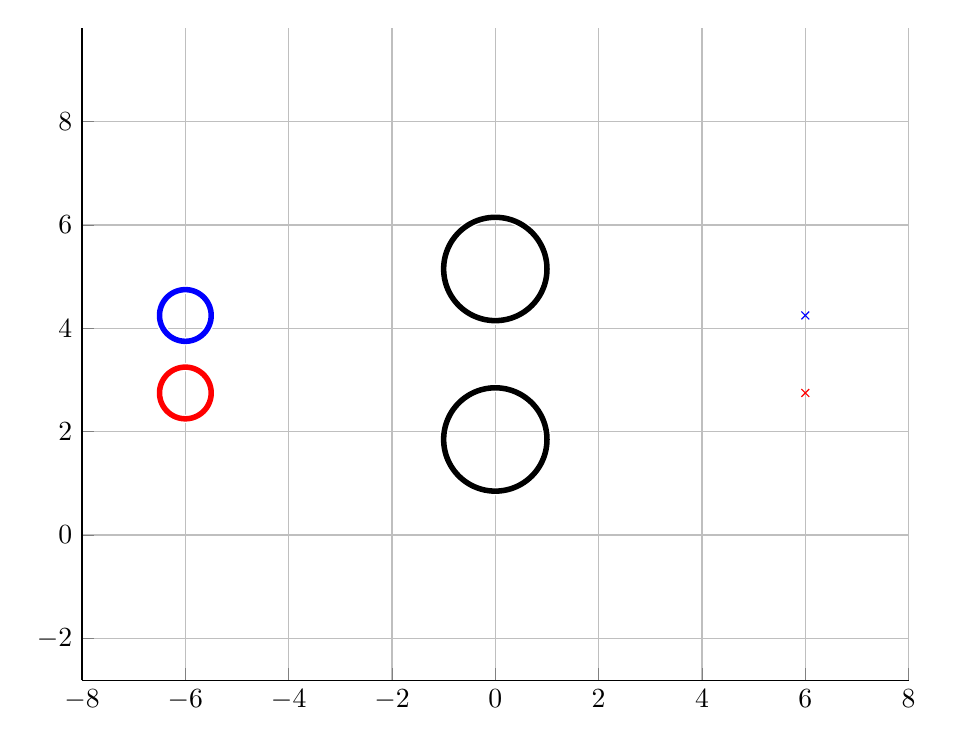
\begin{tikzpicture}

\begin{axis}[%
width=4.133in,
height=3.26in,
at={(0.693in,0.44in)},
scale only axis,
unbounded coords=jump,
xmin=-8,
xmax=8,
xmajorgrids,
ymin=-2.80967741935484,
ymax=9.80967741935484,
ymajorgrids,
axis background/.style={fill=white},
axis x line*=bottom,
axis y line*=left
]
\addplot [color=blue,only marks,mark=x,mark options={solid},forget plot]
  table[row sep=crcr]{%
6	4.25\\
};
\addplot [color=red,only marks,mark=x,mark options={solid},forget plot]
  table[row sep=crcr]{%
6	2.75\\
};
\addplot [color=white,solid,line width=3.0pt,forget plot]
  table[row sep=crcr]{%
-5.5	4.25\\
-5.50030458649045	4.26744974835125\\
-5.50121797487009	4.28487823687206\\
-5.50273905231586	4.30226423163383\\
-5.50486596562921	4.31958655048003\\
-5.5075961234939	4.33682408883347\\
-5.5109261996331	4.35395584540888\\
-5.514852136862	4.37096094779983\\
-5.51936915203084	4.3878186779085\\
-5.52447174185242	4.40450849718747\\
-5.53015368960705	4.42101007166283\\
-5.53640807271661	4.43730329670796\\
-5.5432272711787	4.4533683215379\\
-5.55060297685042	4.46918557339454\\
-5.55852620357054	4.48473578139295\\
-5.56698729810778	4.5\\
-5.57597595192179	4.5149596321166\\
-5.58548121372248	4.52959645173537\\
-5.59549150281253	4.54389262614624\\
-5.60599462319664	4.55783073766283\\
-5.61697777844051	4.57139380484327\\
-5.6284275872613	4.58456530317943\\
-5.64033009983067	4.5973291852295\\
-5.6526708147705	4.60966990016933\\
-5.66543469682057	4.6215724127387\\
-5.67860619515673	4.63302222155949\\
-5.69216926233717	4.64400537680336\\
-5.70610737385376	4.65450849718747\\
-5.72040354826463	4.66451878627752\\
-5.7350403678834	4.67402404807821\\
-5.75	4.68301270189222\\
-5.76526421860705	4.69147379642946\\
-5.78081442660546	4.69939702314958\\
-5.7966316784621	4.7067727288213\\
-5.81269670329204	4.71359192728339\\
-5.82898992833717	4.71984631039295\\
-5.84549150281253	4.72552825814758\\
-5.8621813220915	4.73063084796916\\
-5.87903905220017	4.735147863138\\
-5.89604415459112	4.7390738003669\\
-5.91317591116653	4.7424038765061\\
-5.93041344951997	4.74513403437079\\
-5.94773576836617	4.74726094768414\\
-5.96512176312794	4.74878202512991\\
-5.98255025164875	4.74969541350955\\
-6	4.75\\
-6.01744974835125	4.74969541350955\\
-6.03487823687206	4.74878202512991\\
-6.05226423163383	4.74726094768414\\
-6.06958655048003	4.74513403437079\\
-6.08682408883347	4.7424038765061\\
-6.10395584540888	4.7390738003669\\
-6.12096094779983	4.735147863138\\
-6.1378186779085	4.73063084796916\\
-6.15450849718747	4.72552825814758\\
-6.17101007166283	4.71984631039295\\
-6.18730329670796	4.71359192728339\\
-6.2033683215379	4.7067727288213\\
-6.21918557339454	4.69939702314958\\
-6.23473578139295	4.69147379642946\\
-6.25	4.68301270189222\\
-6.2649596321166	4.67402404807821\\
-6.27959645173537	4.66451878627752\\
-6.29389262614624	4.65450849718747\\
-6.30783073766283	4.64400537680336\\
-6.32139380484327	4.63302222155949\\
-6.33456530317943	4.6215724127387\\
-6.3473291852295	4.60966990016933\\
-6.35966990016933	4.5973291852295\\
-6.3715724127387	4.58456530317943\\
-6.38302222155949	4.57139380484327\\
-6.39400537680336	4.55783073766283\\
-6.40450849718747	4.54389262614624\\
-6.41451878627752	4.52959645173537\\
-6.42402404807821	4.5149596321166\\
-6.43301270189222	4.5\\
-6.44147379642946	4.48473578139295\\
-6.44939702314958	4.46918557339454\\
-6.4567727288213	4.4533683215379\\
-6.46359192728339	4.43730329670796\\
-6.46984631039295	4.42101007166283\\
-6.47552825814758	4.40450849718747\\
-6.48063084796916	4.3878186779085\\
-6.485147863138	4.37096094779983\\
-6.4890738003669	4.35395584540888\\
-6.4924038765061	4.33682408883347\\
-6.49513403437079	4.31958655048003\\
-6.49726094768414	4.30226423163383\\
-6.49878202512991	4.28487823687206\\
-6.49969541350955	4.26744974835125\\
-6.5	4.25\\
-6.49969541350955	4.23255025164875\\
-6.49878202512991	4.21512176312794\\
-6.49726094768414	4.19773576836617\\
-6.49513403437079	4.18041344951997\\
-6.4924038765061	4.16317591116653\\
-6.4890738003669	4.14604415459112\\
-6.485147863138	4.12903905220017\\
-6.48063084796916	4.1121813220915\\
-6.47552825814758	4.09549150281253\\
-6.46984631039295	4.07898992833717\\
-6.46359192728339	4.06269670329204\\
-6.4567727288213	4.0466316784621\\
-6.44939702314958	4.03081442660546\\
-6.44147379642946	4.01526421860705\\
-6.43301270189222	4\\
-6.42402404807821	3.9850403678834\\
-6.41451878627752	3.97040354826463\\
-6.40450849718747	3.95610737385376\\
-6.39400537680336	3.94216926233717\\
-6.38302222155949	3.92860619515673\\
-6.3715724127387	3.91543469682057\\
-6.35966990016933	3.9026708147705\\
-6.3473291852295	3.89033009983067\\
-6.33456530317943	3.8784275872613\\
-6.32139380484327	3.86697777844051\\
-6.30783073766283	3.85599462319664\\
-6.29389262614624	3.84549150281253\\
-6.27959645173537	3.83548121372248\\
-6.2649596321166	3.82597595192179\\
-6.25	3.81698729810778\\
-6.23473578139295	3.80852620357054\\
-6.21918557339454	3.80060297685042\\
-6.2033683215379	3.7932272711787\\
-6.18730329670796	3.78640807271661\\
-6.17101007166283	3.78015368960705\\
-6.15450849718747	3.77447174185242\\
-6.1378186779085	3.76936915203084\\
-6.12096094779983	3.764852136862\\
-6.10395584540888	3.7609261996331\\
-6.08682408883347	3.7575961234939\\
-6.06958655048003	3.75486596562921\\
-6.05226423163383	3.75273905231586\\
-6.03487823687206	3.75121797487009\\
-6.01744974835125	3.75030458649045\\
-6	3.75\\
-5.98255025164875	3.75030458649045\\
-5.96512176312794	3.75121797487009\\
-5.94773576836617	3.75273905231586\\
-5.93041344951997	3.75486596562921\\
-5.91317591116653	3.7575961234939\\
-5.89604415459112	3.7609261996331\\
-5.87903905220017	3.764852136862\\
-5.8621813220915	3.76936915203084\\
-5.84549150281253	3.77447174185242\\
-5.82898992833717	3.78015368960705\\
-5.81269670329204	3.78640807271661\\
-5.7966316784621	3.7932272711787\\
-5.78081442660546	3.80060297685042\\
-5.76526421860705	3.80852620357054\\
-5.75	3.81698729810778\\
-5.7350403678834	3.82597595192179\\
-5.72040354826463	3.83548121372248\\
-5.70610737385376	3.84549150281253\\
-5.69216926233717	3.85599462319664\\
-5.67860619515673	3.86697777844051\\
-5.66543469682057	3.8784275872613\\
-5.6526708147705	3.89033009983067\\
-5.64033009983067	3.9026708147705\\
-5.6284275872613	3.91543469682057\\
-5.61697777844051	3.92860619515673\\
-5.60599462319664	3.94216926233717\\
-5.59549150281253	3.95610737385376\\
-5.58548121372248	3.97040354826463\\
-5.57597595192179	3.9850403678834\\
-5.56698729810778	4\\
-5.55852620357054	4.01526421860705\\
-5.55060297685042	4.03081442660546\\
-5.5432272711787	4.0466316784621\\
-5.53640807271661	4.06269670329204\\
-5.53015368960705	4.07898992833717\\
-5.52447174185242	4.09549150281253\\
-5.51936915203084	4.1121813220915\\
-5.514852136862	4.12903905220017\\
-5.5109261996331	4.14604415459112\\
-5.5075961234939	4.16317591116653\\
-5.50486596562921	4.18041344951997\\
-5.50273905231586	4.19773576836617\\
-5.50121797487009	4.21512176312794\\
-5.50030458649045	4.23255025164875\\
-5.5	4.25\\
nan	nan\\
};
\addplot [color=blue,solid,line width=2.0pt,forget plot]
  table[row sep=crcr]{%
-5.5	4.25\\
-5.50030458649045	4.26744974835125\\
-5.50121797487009	4.28487823687206\\
-5.50273905231586	4.30226423163383\\
-5.50486596562921	4.31958655048003\\
-5.5075961234939	4.33682408883347\\
-5.5109261996331	4.35395584540888\\
-5.514852136862	4.37096094779983\\
-5.51936915203084	4.3878186779085\\
-5.52447174185242	4.40450849718747\\
-5.53015368960705	4.42101007166283\\
-5.53640807271661	4.43730329670796\\
-5.5432272711787	4.4533683215379\\
-5.55060297685042	4.46918557339454\\
-5.55852620357054	4.48473578139295\\
-5.56698729810778	4.5\\
-5.57597595192179	4.5149596321166\\
-5.58548121372248	4.52959645173537\\
-5.59549150281253	4.54389262614624\\
-5.60599462319664	4.55783073766283\\
-5.61697777844051	4.57139380484327\\
-5.6284275872613	4.58456530317943\\
-5.64033009983067	4.5973291852295\\
-5.6526708147705	4.60966990016933\\
-5.66543469682057	4.6215724127387\\
-5.67860619515673	4.63302222155949\\
-5.69216926233717	4.64400537680336\\
-5.70610737385376	4.65450849718747\\
-5.72040354826463	4.66451878627752\\
-5.7350403678834	4.67402404807821\\
-5.75	4.68301270189222\\
-5.76526421860705	4.69147379642946\\
-5.78081442660546	4.69939702314958\\
-5.7966316784621	4.7067727288213\\
-5.81269670329204	4.71359192728339\\
-5.82898992833717	4.71984631039295\\
-5.84549150281253	4.72552825814758\\
-5.8621813220915	4.73063084796916\\
-5.87903905220017	4.735147863138\\
-5.89604415459112	4.7390738003669\\
-5.91317591116653	4.7424038765061\\
-5.93041344951997	4.74513403437079\\
-5.94773576836617	4.74726094768414\\
-5.96512176312794	4.74878202512991\\
-5.98255025164875	4.74969541350955\\
-6	4.75\\
-6.01744974835125	4.74969541350955\\
-6.03487823687206	4.74878202512991\\
-6.05226423163383	4.74726094768414\\
-6.06958655048003	4.74513403437079\\
-6.08682408883347	4.7424038765061\\
-6.10395584540888	4.7390738003669\\
-6.12096094779983	4.735147863138\\
-6.1378186779085	4.73063084796916\\
-6.15450849718747	4.72552825814758\\
-6.17101007166283	4.71984631039295\\
-6.18730329670796	4.71359192728339\\
-6.2033683215379	4.7067727288213\\
-6.21918557339454	4.69939702314958\\
-6.23473578139295	4.69147379642946\\
-6.25	4.68301270189222\\
-6.2649596321166	4.67402404807821\\
-6.27959645173537	4.66451878627752\\
-6.29389262614624	4.65450849718747\\
-6.30783073766283	4.64400537680336\\
-6.32139380484327	4.63302222155949\\
-6.33456530317943	4.6215724127387\\
-6.3473291852295	4.60966990016933\\
-6.35966990016933	4.5973291852295\\
-6.3715724127387	4.58456530317943\\
-6.38302222155949	4.57139380484327\\
-6.39400537680336	4.55783073766283\\
-6.40450849718747	4.54389262614624\\
-6.41451878627752	4.52959645173537\\
-6.42402404807821	4.5149596321166\\
-6.43301270189222	4.5\\
-6.44147379642946	4.48473578139295\\
-6.44939702314958	4.46918557339454\\
-6.4567727288213	4.4533683215379\\
-6.46359192728339	4.43730329670796\\
-6.46984631039295	4.42101007166283\\
-6.47552825814758	4.40450849718747\\
-6.48063084796916	4.3878186779085\\
-6.485147863138	4.37096094779983\\
-6.4890738003669	4.35395584540888\\
-6.4924038765061	4.33682408883347\\
-6.49513403437079	4.31958655048003\\
-6.49726094768414	4.30226423163383\\
-6.49878202512991	4.28487823687206\\
-6.49969541350955	4.26744974835125\\
-6.5	4.25\\
-6.49969541350955	4.23255025164875\\
-6.49878202512991	4.21512176312794\\
-6.49726094768414	4.19773576836617\\
-6.49513403437079	4.18041344951997\\
-6.4924038765061	4.16317591116653\\
-6.4890738003669	4.14604415459112\\
-6.485147863138	4.12903905220017\\
-6.48063084796916	4.1121813220915\\
-6.47552825814758	4.09549150281253\\
-6.46984631039295	4.07898992833717\\
-6.46359192728339	4.06269670329204\\
-6.4567727288213	4.0466316784621\\
-6.44939702314958	4.03081442660546\\
-6.44147379642946	4.01526421860705\\
-6.43301270189222	4\\
-6.42402404807821	3.9850403678834\\
-6.41451878627752	3.97040354826463\\
-6.40450849718747	3.95610737385376\\
-6.39400537680336	3.94216926233717\\
-6.38302222155949	3.92860619515673\\
-6.3715724127387	3.91543469682057\\
-6.35966990016933	3.9026708147705\\
-6.3473291852295	3.89033009983067\\
-6.33456530317943	3.8784275872613\\
-6.32139380484327	3.86697777844051\\
-6.30783073766283	3.85599462319664\\
-6.29389262614624	3.84549150281253\\
-6.27959645173537	3.83548121372248\\
-6.2649596321166	3.82597595192179\\
-6.25	3.81698729810778\\
-6.23473578139295	3.80852620357054\\
-6.21918557339454	3.80060297685042\\
-6.2033683215379	3.7932272711787\\
-6.18730329670796	3.78640807271661\\
-6.17101007166283	3.78015368960705\\
-6.15450849718747	3.77447174185242\\
-6.1378186779085	3.76936915203084\\
-6.12096094779983	3.764852136862\\
-6.10395584540888	3.7609261996331\\
-6.08682408883347	3.7575961234939\\
-6.06958655048003	3.75486596562921\\
-6.05226423163383	3.75273905231586\\
-6.03487823687206	3.75121797487009\\
-6.01744974835125	3.75030458649045\\
-6	3.75\\
-5.98255025164875	3.75030458649045\\
-5.96512176312794	3.75121797487009\\
-5.94773576836617	3.75273905231586\\
-5.93041344951997	3.75486596562921\\
-5.91317591116653	3.7575961234939\\
-5.89604415459112	3.7609261996331\\
-5.87903905220017	3.764852136862\\
-5.8621813220915	3.76936915203084\\
-5.84549150281253	3.77447174185242\\
-5.82898992833717	3.78015368960705\\
-5.81269670329204	3.78640807271661\\
-5.7966316784621	3.7932272711787\\
-5.78081442660546	3.80060297685042\\
-5.76526421860705	3.80852620357054\\
-5.75	3.81698729810778\\
-5.7350403678834	3.82597595192179\\
-5.72040354826463	3.83548121372248\\
-5.70610737385376	3.84549150281253\\
-5.69216926233717	3.85599462319664\\
-5.67860619515673	3.86697777844051\\
-5.66543469682057	3.8784275872613\\
-5.6526708147705	3.89033009983067\\
-5.64033009983067	3.9026708147705\\
-5.6284275872613	3.91543469682057\\
-5.61697777844051	3.92860619515673\\
-5.60599462319664	3.94216926233717\\
-5.59549150281253	3.95610737385376\\
-5.58548121372248	3.97040354826463\\
-5.57597595192179	3.9850403678834\\
-5.56698729810778	4\\
-5.55852620357054	4.01526421860705\\
-5.55060297685042	4.03081442660546\\
-5.5432272711787	4.0466316784621\\
-5.53640807271661	4.06269670329204\\
-5.53015368960705	4.07898992833717\\
-5.52447174185242	4.09549150281253\\
-5.51936915203084	4.1121813220915\\
-5.514852136862	4.12903905220017\\
-5.5109261996331	4.14604415459112\\
-5.5075961234939	4.16317591116653\\
-5.50486596562921	4.18041344951997\\
-5.50273905231586	4.19773576836617\\
-5.50121797487009	4.21512176312794\\
-5.50030458649045	4.23255025164875\\
-5.5	4.25\\
nan	nan\\
};
\addplot [color=white,solid,line width=3.0pt,forget plot]
  table[row sep=crcr]{%
-5.5	2.75\\
-5.50030458649045	2.76744974835125\\
-5.50121797487009	2.78487823687206\\
-5.50273905231586	2.80226423163383\\
-5.50486596562921	2.81958655048003\\
-5.5075961234939	2.83682408883347\\
-5.5109261996331	2.85395584540888\\
-5.514852136862	2.87096094779983\\
-5.51936915203084	2.8878186779085\\
-5.52447174185242	2.90450849718747\\
-5.53015368960705	2.92101007166283\\
-5.53640807271661	2.93730329670796\\
-5.5432272711787	2.9533683215379\\
-5.55060297685042	2.96918557339454\\
-5.55852620357054	2.98473578139295\\
-5.56698729810778	3\\
-5.57597595192179	3.0149596321166\\
-5.58548121372248	3.02959645173537\\
-5.59549150281253	3.04389262614624\\
-5.60599462319664	3.05783073766283\\
-5.61697777844051	3.07139380484327\\
-5.6284275872613	3.08456530317943\\
-5.64033009983067	3.0973291852295\\
-5.6526708147705	3.10966990016933\\
-5.66543469682057	3.1215724127387\\
-5.67860619515673	3.13302222155949\\
-5.69216926233717	3.14400537680336\\
-5.70610737385376	3.15450849718747\\
-5.72040354826463	3.16451878627752\\
-5.7350403678834	3.17402404807821\\
-5.75	3.18301270189222\\
-5.76526421860705	3.19147379642946\\
-5.78081442660546	3.19939702314958\\
-5.7966316784621	3.2067727288213\\
-5.81269670329204	3.21359192728339\\
-5.82898992833717	3.21984631039295\\
-5.84549150281253	3.22552825814758\\
-5.8621813220915	3.23063084796916\\
-5.87903905220017	3.235147863138\\
-5.89604415459112	3.2390738003669\\
-5.91317591116653	3.2424038765061\\
-5.93041344951997	3.24513403437079\\
-5.94773576836617	3.24726094768414\\
-5.96512176312794	3.24878202512991\\
-5.98255025164875	3.24969541350955\\
-6	3.25\\
-6.01744974835125	3.24969541350955\\
-6.03487823687206	3.24878202512991\\
-6.05226423163383	3.24726094768414\\
-6.06958655048003	3.24513403437079\\
-6.08682408883347	3.2424038765061\\
-6.10395584540888	3.2390738003669\\
-6.12096094779983	3.235147863138\\
-6.1378186779085	3.23063084796916\\
-6.15450849718747	3.22552825814758\\
-6.17101007166283	3.21984631039295\\
-6.18730329670796	3.21359192728339\\
-6.2033683215379	3.2067727288213\\
-6.21918557339454	3.19939702314958\\
-6.23473578139295	3.19147379642946\\
-6.25	3.18301270189222\\
-6.2649596321166	3.17402404807821\\
-6.27959645173537	3.16451878627752\\
-6.29389262614624	3.15450849718747\\
-6.30783073766283	3.14400537680336\\
-6.32139380484327	3.13302222155949\\
-6.33456530317943	3.1215724127387\\
-6.3473291852295	3.10966990016933\\
-6.35966990016933	3.0973291852295\\
-6.3715724127387	3.08456530317943\\
-6.38302222155949	3.07139380484327\\
-6.39400537680336	3.05783073766283\\
-6.40450849718747	3.04389262614624\\
-6.41451878627752	3.02959645173537\\
-6.42402404807821	3.0149596321166\\
-6.43301270189222	3\\
-6.44147379642946	2.98473578139295\\
-6.44939702314958	2.96918557339454\\
-6.4567727288213	2.9533683215379\\
-6.46359192728339	2.93730329670796\\
-6.46984631039295	2.92101007166283\\
-6.47552825814758	2.90450849718747\\
-6.48063084796916	2.8878186779085\\
-6.485147863138	2.87096094779983\\
-6.4890738003669	2.85395584540888\\
-6.4924038765061	2.83682408883347\\
-6.49513403437079	2.81958655048003\\
-6.49726094768414	2.80226423163383\\
-6.49878202512991	2.78487823687206\\
-6.49969541350955	2.76744974835125\\
-6.5	2.75\\
-6.49969541350955	2.73255025164875\\
-6.49878202512991	2.71512176312794\\
-6.49726094768414	2.69773576836617\\
-6.49513403437079	2.68041344951997\\
-6.4924038765061	2.66317591116653\\
-6.4890738003669	2.64604415459112\\
-6.485147863138	2.62903905220017\\
-6.48063084796916	2.6121813220915\\
-6.47552825814758	2.59549150281253\\
-6.46984631039295	2.57898992833717\\
-6.46359192728339	2.56269670329204\\
-6.4567727288213	2.5466316784621\\
-6.44939702314958	2.53081442660546\\
-6.44147379642946	2.51526421860705\\
-6.43301270189222	2.5\\
-6.42402404807821	2.4850403678834\\
-6.41451878627752	2.47040354826463\\
-6.40450849718747	2.45610737385376\\
-6.39400537680336	2.44216926233717\\
-6.38302222155949	2.42860619515673\\
-6.3715724127387	2.41543469682057\\
-6.35966990016933	2.4026708147705\\
-6.3473291852295	2.39033009983067\\
-6.33456530317943	2.3784275872613\\
-6.32139380484327	2.36697777844051\\
-6.30783073766283	2.35599462319664\\
-6.29389262614624	2.34549150281253\\
-6.27959645173537	2.33548121372248\\
-6.2649596321166	2.32597595192179\\
-6.25	2.31698729810778\\
-6.23473578139295	2.30852620357054\\
-6.21918557339454	2.30060297685042\\
-6.2033683215379	2.2932272711787\\
-6.18730329670796	2.28640807271661\\
-6.17101007166283	2.28015368960705\\
-6.15450849718747	2.27447174185242\\
-6.1378186779085	2.26936915203084\\
-6.12096094779983	2.264852136862\\
-6.10395584540888	2.2609261996331\\
-6.08682408883347	2.2575961234939\\
-6.06958655048003	2.25486596562921\\
-6.05226423163383	2.25273905231586\\
-6.03487823687206	2.25121797487009\\
-6.01744974835125	2.25030458649045\\
-6	2.25\\
-5.98255025164875	2.25030458649045\\
-5.96512176312794	2.25121797487009\\
-5.94773576836617	2.25273905231586\\
-5.93041344951997	2.25486596562921\\
-5.91317591116653	2.2575961234939\\
-5.89604415459112	2.2609261996331\\
-5.87903905220017	2.264852136862\\
-5.8621813220915	2.26936915203084\\
-5.84549150281253	2.27447174185242\\
-5.82898992833717	2.28015368960705\\
-5.81269670329204	2.28640807271661\\
-5.7966316784621	2.2932272711787\\
-5.78081442660546	2.30060297685042\\
-5.76526421860705	2.30852620357054\\
-5.75	2.31698729810778\\
-5.7350403678834	2.32597595192179\\
-5.72040354826463	2.33548121372248\\
-5.70610737385376	2.34549150281253\\
-5.69216926233717	2.35599462319664\\
-5.67860619515673	2.36697777844051\\
-5.66543469682057	2.3784275872613\\
-5.6526708147705	2.39033009983067\\
-5.64033009983067	2.4026708147705\\
-5.6284275872613	2.41543469682057\\
-5.61697777844051	2.42860619515673\\
-5.60599462319664	2.44216926233717\\
-5.59549150281253	2.45610737385376\\
-5.58548121372248	2.47040354826463\\
-5.57597595192179	2.4850403678834\\
-5.56698729810778	2.5\\
-5.55852620357054	2.51526421860705\\
-5.55060297685042	2.53081442660546\\
-5.5432272711787	2.5466316784621\\
-5.53640807271661	2.56269670329204\\
-5.53015368960705	2.57898992833717\\
-5.52447174185242	2.59549150281253\\
-5.51936915203084	2.6121813220915\\
-5.514852136862	2.62903905220017\\
-5.5109261996331	2.64604415459112\\
-5.5075961234939	2.66317591116653\\
-5.50486596562921	2.68041344951997\\
-5.50273905231586	2.69773576836617\\
-5.50121797487009	2.71512176312794\\
-5.50030458649045	2.73255025164875\\
-5.5	2.75\\
nan	nan\\
};
\addplot [color=red,solid,line width=2.0pt,forget plot]
  table[row sep=crcr]{%
-5.5	2.75\\
-5.50030458649045	2.76744974835125\\
-5.50121797487009	2.78487823687206\\
-5.50273905231586	2.80226423163383\\
-5.50486596562921	2.81958655048003\\
-5.5075961234939	2.83682408883347\\
-5.5109261996331	2.85395584540888\\
-5.514852136862	2.87096094779983\\
-5.51936915203084	2.8878186779085\\
-5.52447174185242	2.90450849718747\\
-5.53015368960705	2.92101007166283\\
-5.53640807271661	2.93730329670796\\
-5.5432272711787	2.9533683215379\\
-5.55060297685042	2.96918557339454\\
-5.55852620357054	2.98473578139295\\
-5.56698729810778	3\\
-5.57597595192179	3.0149596321166\\
-5.58548121372248	3.02959645173537\\
-5.59549150281253	3.04389262614624\\
-5.60599462319664	3.05783073766283\\
-5.61697777844051	3.07139380484327\\
-5.6284275872613	3.08456530317943\\
-5.64033009983067	3.0973291852295\\
-5.6526708147705	3.10966990016933\\
-5.66543469682057	3.1215724127387\\
-5.67860619515673	3.13302222155949\\
-5.69216926233717	3.14400537680336\\
-5.70610737385376	3.15450849718747\\
-5.72040354826463	3.16451878627752\\
-5.7350403678834	3.17402404807821\\
-5.75	3.18301270189222\\
-5.76526421860705	3.19147379642946\\
-5.78081442660546	3.19939702314958\\
-5.7966316784621	3.2067727288213\\
-5.81269670329204	3.21359192728339\\
-5.82898992833717	3.21984631039295\\
-5.84549150281253	3.22552825814758\\
-5.8621813220915	3.23063084796916\\
-5.87903905220017	3.235147863138\\
-5.89604415459112	3.2390738003669\\
-5.91317591116653	3.2424038765061\\
-5.93041344951997	3.24513403437079\\
-5.94773576836617	3.24726094768414\\
-5.96512176312794	3.24878202512991\\
-5.98255025164875	3.24969541350955\\
-6	3.25\\
-6.01744974835125	3.24969541350955\\
-6.03487823687206	3.24878202512991\\
-6.05226423163383	3.24726094768414\\
-6.06958655048003	3.24513403437079\\
-6.08682408883347	3.2424038765061\\
-6.10395584540888	3.2390738003669\\
-6.12096094779983	3.235147863138\\
-6.1378186779085	3.23063084796916\\
-6.15450849718747	3.22552825814758\\
-6.17101007166283	3.21984631039295\\
-6.18730329670796	3.21359192728339\\
-6.2033683215379	3.2067727288213\\
-6.21918557339454	3.19939702314958\\
-6.23473578139295	3.19147379642946\\
-6.25	3.18301270189222\\
-6.2649596321166	3.17402404807821\\
-6.27959645173537	3.16451878627752\\
-6.29389262614624	3.15450849718747\\
-6.30783073766283	3.14400537680336\\
-6.32139380484327	3.13302222155949\\
-6.33456530317943	3.1215724127387\\
-6.3473291852295	3.10966990016933\\
-6.35966990016933	3.0973291852295\\
-6.3715724127387	3.08456530317943\\
-6.38302222155949	3.07139380484327\\
-6.39400537680336	3.05783073766283\\
-6.40450849718747	3.04389262614624\\
-6.41451878627752	3.02959645173537\\
-6.42402404807821	3.0149596321166\\
-6.43301270189222	3\\
-6.44147379642946	2.98473578139295\\
-6.44939702314958	2.96918557339454\\
-6.4567727288213	2.9533683215379\\
-6.46359192728339	2.93730329670796\\
-6.46984631039295	2.92101007166283\\
-6.47552825814758	2.90450849718747\\
-6.48063084796916	2.8878186779085\\
-6.485147863138	2.87096094779983\\
-6.4890738003669	2.85395584540888\\
-6.4924038765061	2.83682408883347\\
-6.49513403437079	2.81958655048003\\
-6.49726094768414	2.80226423163383\\
-6.49878202512991	2.78487823687206\\
-6.49969541350955	2.76744974835125\\
-6.5	2.75\\
-6.49969541350955	2.73255025164875\\
-6.49878202512991	2.71512176312794\\
-6.49726094768414	2.69773576836617\\
-6.49513403437079	2.68041344951997\\
-6.4924038765061	2.66317591116653\\
-6.4890738003669	2.64604415459112\\
-6.485147863138	2.62903905220017\\
-6.48063084796916	2.6121813220915\\
-6.47552825814758	2.59549150281253\\
-6.46984631039295	2.57898992833717\\
-6.46359192728339	2.56269670329204\\
-6.4567727288213	2.5466316784621\\
-6.44939702314958	2.53081442660546\\
-6.44147379642946	2.51526421860705\\
-6.43301270189222	2.5\\
-6.42402404807821	2.4850403678834\\
-6.41451878627752	2.47040354826463\\
-6.40450849718747	2.45610737385376\\
-6.39400537680336	2.44216926233717\\
-6.38302222155949	2.42860619515673\\
-6.3715724127387	2.41543469682057\\
-6.35966990016933	2.4026708147705\\
-6.3473291852295	2.39033009983067\\
-6.33456530317943	2.3784275872613\\
-6.32139380484327	2.36697777844051\\
-6.30783073766283	2.35599462319664\\
-6.29389262614624	2.34549150281253\\
-6.27959645173537	2.33548121372248\\
-6.2649596321166	2.32597595192179\\
-6.25	2.31698729810778\\
-6.23473578139295	2.30852620357054\\
-6.21918557339454	2.30060297685042\\
-6.2033683215379	2.2932272711787\\
-6.18730329670796	2.28640807271661\\
-6.17101007166283	2.28015368960705\\
-6.15450849718747	2.27447174185242\\
-6.1378186779085	2.26936915203084\\
-6.12096094779983	2.264852136862\\
-6.10395584540888	2.2609261996331\\
-6.08682408883347	2.2575961234939\\
-6.06958655048003	2.25486596562921\\
-6.05226423163383	2.25273905231586\\
-6.03487823687206	2.25121797487009\\
-6.01744974835125	2.25030458649045\\
-6	2.25\\
-5.98255025164875	2.25030458649045\\
-5.96512176312794	2.25121797487009\\
-5.94773576836617	2.25273905231586\\
-5.93041344951997	2.25486596562921\\
-5.91317591116653	2.2575961234939\\
-5.89604415459112	2.2609261996331\\
-5.87903905220017	2.264852136862\\
-5.8621813220915	2.26936915203084\\
-5.84549150281253	2.27447174185242\\
-5.82898992833717	2.28015368960705\\
-5.81269670329204	2.28640807271661\\
-5.7966316784621	2.2932272711787\\
-5.78081442660546	2.30060297685042\\
-5.76526421860705	2.30852620357054\\
-5.75	2.31698729810778\\
-5.7350403678834	2.32597595192179\\
-5.72040354826463	2.33548121372248\\
-5.70610737385376	2.34549150281253\\
-5.69216926233717	2.35599462319664\\
-5.67860619515673	2.36697777844051\\
-5.66543469682057	2.3784275872613\\
-5.6526708147705	2.39033009983067\\
-5.64033009983067	2.4026708147705\\
-5.6284275872613	2.41543469682057\\
-5.61697777844051	2.42860619515673\\
-5.60599462319664	2.44216926233717\\
-5.59549150281253	2.45610737385376\\
-5.58548121372248	2.47040354826463\\
-5.57597595192179	2.4850403678834\\
-5.56698729810778	2.5\\
-5.55852620357054	2.51526421860705\\
-5.55060297685042	2.53081442660546\\
-5.5432272711787	2.5466316784621\\
-5.53640807271661	2.56269670329204\\
-5.53015368960705	2.57898992833717\\
-5.52447174185242	2.59549150281253\\
-5.51936915203084	2.6121813220915\\
-5.514852136862	2.62903905220017\\
-5.5109261996331	2.64604415459112\\
-5.5075961234939	2.66317591116653\\
-5.50486596562921	2.68041344951997\\
-5.50273905231586	2.69773576836617\\
-5.50121797487009	2.71512176312794\\
-5.50030458649045	2.73255025164875\\
-5.5	2.75\\
nan	nan\\
};
\addplot [color=white,solid,line width=3.0pt,forget plot]
  table[row sep=crcr]{%
1	1.85\\
0.999390827019096	1.8848994967025\\
0.997564050259824	1.91975647374413\\
0.994521895368273	1.95452846326765\\
0.99026806874157	1.98917310096007\\
0.984807753012208	2.02364817766693\\
0.978147600733806	2.05791169081776\\
0.970295726275996	2.09192189559967\\
0.961261695938319	2.125637355817\\
0.951056516295154	2.15901699437495\\
0.939692620785908	2.19202014332567\\
0.927183854566787	2.22460659341591\\
0.913545457642601	2.2567366430758\\
0.898794046299167	2.28837114678908\\
0.882947592858927	2.31947156278589\\
0.866025403784439	2.35\\
0.848048096156426	2.37991926423321\\
0.829037572555042	2.40919290347075\\
0.809016994374947	2.43778525229247\\
0.788010753606722	2.46566147532566\\
0.766044443118978	2.49278760968654\\
0.743144825477394	2.51913060635886\\
0.719339800338651	2.544658370459\\
0.694658370458997	2.56933980033865\\
0.669130606358858	2.59314482547739\\
0.642787609686539	2.61604444311898\\
0.615661475325658	2.63801075360672\\
0.587785252292473	2.65901699437495\\
0.559192903470747	2.67903757255504\\
0.529919264233205	2.69804809615643\\
0.5	2.71602540378444\\
0.469471562785891	2.73294759285893\\
0.438371146789077	2.74879404629917\\
0.4067366430758	2.7635454576426\\
0.374606593415912	2.77718385456679\\
0.342020143325669	2.78969262078591\\
0.309016994374947	2.80105651629515\\
0.275637355816999	2.81126169593832\\
0.241921895599668	2.820295726276\\
0.207911690817759	2.82814760073381\\
0.17364817766693	2.83480775301221\\
0.139173100960066	2.84026806874157\\
0.104528463267653	2.84452189536827\\
0.0697564737441255	2.84756405025982\\
0.0348994967025011	2.8493908270191\\
6.12323399573677e-17	2.85\\
-0.0348994967025007	2.8493908270191\\
-0.0697564737441253	2.84756405025982\\
-0.104528463267653	2.84452189536827\\
-0.139173100960065	2.84026806874157\\
-0.17364817766693	2.83480775301221\\
-0.207911690817759	2.82814760073381\\
-0.241921895599668	2.820295726276\\
-0.275637355816999	2.81126169593832\\
-0.309016994374947	2.80105651629515\\
-0.342020143325669	2.78969262078591\\
-0.374606593415912	2.77718385456679\\
-0.4067366430758	2.7635454576426\\
-0.438371146789078	2.74879404629917\\
-0.469471562785891	2.73294759285893\\
-0.5	2.71602540378444\\
-0.529919264233205	2.69804809615643\\
-0.559192903470747	2.67903757255504\\
-0.587785252292473	2.65901699437495\\
-0.615661475325658	2.63801075360672\\
-0.642787609686539	2.61604444311898\\
-0.669130606358858	2.59314482547739\\
-0.694658370458997	2.56933980033865\\
-0.719339800338651	2.544658370459\\
-0.743144825477394	2.51913060635886\\
-0.766044443118978	2.49278760968654\\
-0.788010753606722	2.46566147532566\\
-0.809016994374947	2.43778525229247\\
-0.829037572555042	2.40919290347075\\
-0.848048096156426	2.37991926423321\\
-0.866025403784439	2.35\\
-0.882947592858927	2.31947156278589\\
-0.898794046299167	2.28837114678908\\
-0.913545457642601	2.2567366430758\\
-0.927183854566787	2.22460659341591\\
-0.939692620785908	2.19202014332567\\
-0.951056516295154	2.15901699437495\\
-0.961261695938319	2.125637355817\\
-0.970295726275996	2.09192189559967\\
-0.978147600733806	2.05791169081776\\
-0.984807753012208	2.02364817766693\\
-0.99026806874157	1.98917310096007\\
-0.994521895368273	1.95452846326765\\
-0.997564050259824	1.91975647374413\\
-0.999390827019096	1.8848994967025\\
-1	1.85\\
-0.999390827019096	1.8151005032975\\
-0.997564050259824	1.78024352625588\\
-0.994521895368273	1.74547153673235\\
-0.99026806874157	1.71082689903993\\
-0.984807753012208	1.67635182233307\\
-0.978147600733806	1.64208830918224\\
-0.970295726275997	1.60807810440033\\
-0.961261695938319	1.574362644183\\
-0.951056516295154	1.54098300562505\\
-0.939692620785908	1.50797985667433\\
-0.927183854566787	1.47539340658409\\
-0.913545457642601	1.4432633569242\\
-0.898794046299167	1.41162885321092\\
-0.882947592858927	1.38052843721411\\
-0.866025403784439	1.35\\
-0.848048096156426	1.3200807357668\\
-0.829037572555042	1.29080709652925\\
-0.809016994374947	1.26221474770753\\
-0.788010753606722	1.23433852467434\\
-0.766044443118978	1.20721239031346\\
-0.743144825477394	1.18086939364114\\
-0.719339800338651	1.155341629541\\
-0.694658370458997	1.13066019966135\\
-0.669130606358858	1.10685517452261\\
-0.642787609686539	1.08395555688102\\
-0.615661475325658	1.06198924639328\\
-0.587785252292473	1.04098300562505\\
-0.559192903470747	1.02096242744496\\
-0.529919264233205	1.00195190384357\\
-0.5	0.983974596215562\\
-0.469471562785891	0.967052407141073\\
-0.438371146789078	0.951205953700833\\
-0.4067366430758	0.936454542357399\\
-0.374606593415912	0.922816145433213\\
-0.342020143325669	0.910307379214092\\
-0.309016994374948	0.898943483704847\\
-0.275637355816999	0.888738304061681\\
-0.241921895599668	0.879704273724004\\
-0.20791169081776	0.871852399266195\\
-0.17364817766693	0.865192246987792\\
-0.139173100960065	0.85973193125843\\
-0.104528463267653	0.855478104631727\\
-0.0697564737441256	0.852435949740176\\
-0.0348994967025016	0.850609172980904\\
-1.83697019872103e-16	0.85\\
0.0348994967025013	0.850609172980904\\
0.0697564737441252	0.852435949740176\\
0.104528463267653	0.855478104631727\\
0.139173100960065	0.85973193125843\\
0.17364817766693	0.865192246987792\\
0.207911690817759	0.871852399266194\\
0.241921895599667	0.879704273724004\\
0.275637355816999	0.888738304061681\\
0.309016994374947	0.898943483704846\\
0.342020143325668	0.910307379214092\\
0.374606593415912	0.922816145433213\\
0.406736643075801	0.936454542357399\\
0.438371146789077	0.951205953700833\\
0.46947156278589	0.967052407141073\\
0.5	0.983974596215561\\
0.529919264233205	1.00195190384357\\
0.559192903470746	1.02096242744496\\
0.587785252292473	1.04098300562505\\
0.615661475325659	1.06198924639328\\
0.642787609686539	1.08395555688102\\
0.669130606358858	1.10685517452261\\
0.694658370458997	1.13066019966135\\
0.719339800338651	1.155341629541\\
0.743144825477394	1.18086939364114\\
0.766044443118978	1.20721239031346\\
0.788010753606722	1.23433852467434\\
0.809016994374947	1.26221474770753\\
0.829037572555041	1.29080709652925\\
0.848048096156425	1.32008073576679\\
0.866025403784438	1.35\\
0.882947592858927	1.38052843721411\\
0.898794046299167	1.41162885321092\\
0.913545457642601	1.4432633569242\\
0.927183854566787	1.47539340658409\\
0.939692620785908	1.50797985667433\\
0.951056516295154	1.54098300562505\\
0.961261695938319	1.574362644183\\
0.970295726275996	1.60807810440033\\
0.978147600733806	1.64208830918224\\
0.984807753012208	1.67635182233307\\
0.99026806874157	1.71082689903993\\
0.994521895368273	1.74547153673235\\
0.997564050259824	1.78024352625588\\
0.999390827019096	1.8151005032975\\
1	1.85\\
nan	nan\\
};
\addplot [color=black,solid,line width=2.0pt,forget plot]
  table[row sep=crcr]{%
1	1.85\\
0.999390827019096	1.8848994967025\\
0.997564050259824	1.91975647374413\\
0.994521895368273	1.95452846326765\\
0.99026806874157	1.98917310096007\\
0.984807753012208	2.02364817766693\\
0.978147600733806	2.05791169081776\\
0.970295726275996	2.09192189559967\\
0.961261695938319	2.125637355817\\
0.951056516295154	2.15901699437495\\
0.939692620785908	2.19202014332567\\
0.927183854566787	2.22460659341591\\
0.913545457642601	2.2567366430758\\
0.898794046299167	2.28837114678908\\
0.882947592858927	2.31947156278589\\
0.866025403784439	2.35\\
0.848048096156426	2.37991926423321\\
0.829037572555042	2.40919290347075\\
0.809016994374947	2.43778525229247\\
0.788010753606722	2.46566147532566\\
0.766044443118978	2.49278760968654\\
0.743144825477394	2.51913060635886\\
0.719339800338651	2.544658370459\\
0.694658370458997	2.56933980033865\\
0.669130606358858	2.59314482547739\\
0.642787609686539	2.61604444311898\\
0.615661475325658	2.63801075360672\\
0.587785252292473	2.65901699437495\\
0.559192903470747	2.67903757255504\\
0.529919264233205	2.69804809615643\\
0.5	2.71602540378444\\
0.469471562785891	2.73294759285893\\
0.438371146789077	2.74879404629917\\
0.4067366430758	2.7635454576426\\
0.374606593415912	2.77718385456679\\
0.342020143325669	2.78969262078591\\
0.309016994374947	2.80105651629515\\
0.275637355816999	2.81126169593832\\
0.241921895599668	2.820295726276\\
0.207911690817759	2.82814760073381\\
0.17364817766693	2.83480775301221\\
0.139173100960066	2.84026806874157\\
0.104528463267653	2.84452189536827\\
0.0697564737441255	2.84756405025982\\
0.0348994967025011	2.8493908270191\\
6.12323399573677e-17	2.85\\
-0.0348994967025007	2.8493908270191\\
-0.0697564737441253	2.84756405025982\\
-0.104528463267653	2.84452189536827\\
-0.139173100960065	2.84026806874157\\
-0.17364817766693	2.83480775301221\\
-0.207911690817759	2.82814760073381\\
-0.241921895599668	2.820295726276\\
-0.275637355816999	2.81126169593832\\
-0.309016994374947	2.80105651629515\\
-0.342020143325669	2.78969262078591\\
-0.374606593415912	2.77718385456679\\
-0.4067366430758	2.7635454576426\\
-0.438371146789078	2.74879404629917\\
-0.469471562785891	2.73294759285893\\
-0.5	2.71602540378444\\
-0.529919264233205	2.69804809615643\\
-0.559192903470747	2.67903757255504\\
-0.587785252292473	2.65901699437495\\
-0.615661475325658	2.63801075360672\\
-0.642787609686539	2.61604444311898\\
-0.669130606358858	2.59314482547739\\
-0.694658370458997	2.56933980033865\\
-0.719339800338651	2.544658370459\\
-0.743144825477394	2.51913060635886\\
-0.766044443118978	2.49278760968654\\
-0.788010753606722	2.46566147532566\\
-0.809016994374947	2.43778525229247\\
-0.829037572555042	2.40919290347075\\
-0.848048096156426	2.37991926423321\\
-0.866025403784439	2.35\\
-0.882947592858927	2.31947156278589\\
-0.898794046299167	2.28837114678908\\
-0.913545457642601	2.2567366430758\\
-0.927183854566787	2.22460659341591\\
-0.939692620785908	2.19202014332567\\
-0.951056516295154	2.15901699437495\\
-0.961261695938319	2.125637355817\\
-0.970295726275996	2.09192189559967\\
-0.978147600733806	2.05791169081776\\
-0.984807753012208	2.02364817766693\\
-0.99026806874157	1.98917310096007\\
-0.994521895368273	1.95452846326765\\
-0.997564050259824	1.91975647374413\\
-0.999390827019096	1.8848994967025\\
-1	1.85\\
-0.999390827019096	1.8151005032975\\
-0.997564050259824	1.78024352625588\\
-0.994521895368273	1.74547153673235\\
-0.99026806874157	1.71082689903993\\
-0.984807753012208	1.67635182233307\\
-0.978147600733806	1.64208830918224\\
-0.970295726275997	1.60807810440033\\
-0.961261695938319	1.574362644183\\
-0.951056516295154	1.54098300562505\\
-0.939692620785908	1.50797985667433\\
-0.927183854566787	1.47539340658409\\
-0.913545457642601	1.4432633569242\\
-0.898794046299167	1.41162885321092\\
-0.882947592858927	1.38052843721411\\
-0.866025403784439	1.35\\
-0.848048096156426	1.3200807357668\\
-0.829037572555042	1.29080709652925\\
-0.809016994374947	1.26221474770753\\
-0.788010753606722	1.23433852467434\\
-0.766044443118978	1.20721239031346\\
-0.743144825477394	1.18086939364114\\
-0.719339800338651	1.155341629541\\
-0.694658370458997	1.13066019966135\\
-0.669130606358858	1.10685517452261\\
-0.642787609686539	1.08395555688102\\
-0.615661475325658	1.06198924639328\\
-0.587785252292473	1.04098300562505\\
-0.559192903470747	1.02096242744496\\
-0.529919264233205	1.00195190384357\\
-0.5	0.983974596215562\\
-0.469471562785891	0.967052407141073\\
-0.438371146789078	0.951205953700833\\
-0.4067366430758	0.936454542357399\\
-0.374606593415912	0.922816145433213\\
-0.342020143325669	0.910307379214092\\
-0.309016994374948	0.898943483704847\\
-0.275637355816999	0.888738304061681\\
-0.241921895599668	0.879704273724004\\
-0.20791169081776	0.871852399266195\\
-0.17364817766693	0.865192246987792\\
-0.139173100960065	0.85973193125843\\
-0.104528463267653	0.855478104631727\\
-0.0697564737441256	0.852435949740176\\
-0.0348994967025016	0.850609172980904\\
-1.83697019872103e-16	0.85\\
0.0348994967025013	0.850609172980904\\
0.0697564737441252	0.852435949740176\\
0.104528463267653	0.855478104631727\\
0.139173100960065	0.85973193125843\\
0.17364817766693	0.865192246987792\\
0.207911690817759	0.871852399266194\\
0.241921895599667	0.879704273724004\\
0.275637355816999	0.888738304061681\\
0.309016994374947	0.898943483704846\\
0.342020143325668	0.910307379214092\\
0.374606593415912	0.922816145433213\\
0.406736643075801	0.936454542357399\\
0.438371146789077	0.951205953700833\\
0.46947156278589	0.967052407141073\\
0.5	0.983974596215561\\
0.529919264233205	1.00195190384357\\
0.559192903470746	1.02096242744496\\
0.587785252292473	1.04098300562505\\
0.615661475325659	1.06198924639328\\
0.642787609686539	1.08395555688102\\
0.669130606358858	1.10685517452261\\
0.694658370458997	1.13066019966135\\
0.719339800338651	1.155341629541\\
0.743144825477394	1.18086939364114\\
0.766044443118978	1.20721239031346\\
0.788010753606722	1.23433852467434\\
0.809016994374947	1.26221474770753\\
0.829037572555041	1.29080709652925\\
0.848048096156425	1.32008073576679\\
0.866025403784438	1.35\\
0.882947592858927	1.38052843721411\\
0.898794046299167	1.41162885321092\\
0.913545457642601	1.4432633569242\\
0.927183854566787	1.47539340658409\\
0.939692620785908	1.50797985667433\\
0.951056516295154	1.54098300562505\\
0.961261695938319	1.574362644183\\
0.970295726275996	1.60807810440033\\
0.978147600733806	1.64208830918224\\
0.984807753012208	1.67635182233307\\
0.99026806874157	1.71082689903993\\
0.994521895368273	1.74547153673235\\
0.997564050259824	1.78024352625588\\
0.999390827019096	1.8151005032975\\
1	1.85\\
nan	nan\\
};
\addplot [color=white,solid,line width=3.0pt,forget plot]
  table[row sep=crcr]{%
1	5.15\\
0.999390827019096	5.1848994967025\\
0.997564050259824	5.21975647374413\\
0.994521895368273	5.25452846326765\\
0.99026806874157	5.28917310096007\\
0.984807753012208	5.32364817766693\\
0.978147600733806	5.35791169081776\\
0.970295726275996	5.39192189559967\\
0.961261695938319	5.425637355817\\
0.951056516295154	5.45901699437495\\
0.939692620785908	5.49202014332567\\
0.927183854566787	5.52460659341591\\
0.913545457642601	5.5567366430758\\
0.898794046299167	5.58837114678908\\
0.882947592858927	5.61947156278589\\
0.866025403784439	5.65\\
0.848048096156426	5.67991926423321\\
0.829037572555042	5.70919290347075\\
0.809016994374947	5.73778525229247\\
0.788010753606722	5.76566147532566\\
0.766044443118978	5.79278760968654\\
0.743144825477394	5.81913060635886\\
0.719339800338651	5.844658370459\\
0.694658370458997	5.86933980033865\\
0.669130606358858	5.89314482547739\\
0.642787609686539	5.91604444311898\\
0.615661475325658	5.93801075360672\\
0.587785252292473	5.95901699437495\\
0.559192903470747	5.97903757255504\\
0.529919264233205	5.99804809615643\\
0.5	6.01602540378444\\
0.469471562785891	6.03294759285893\\
0.438371146789077	6.04879404629917\\
0.4067366430758	6.0635454576426\\
0.374606593415912	6.07718385456679\\
0.342020143325669	6.08969262078591\\
0.309016994374947	6.10105651629515\\
0.275637355816999	6.11126169593832\\
0.241921895599668	6.120295726276\\
0.207911690817759	6.12814760073381\\
0.17364817766693	6.13480775301221\\
0.139173100960066	6.14026806874157\\
0.104528463267653	6.14452189536827\\
0.0697564737441255	6.14756405025982\\
0.0348994967025011	6.1493908270191\\
6.12323399573677e-17	6.15\\
-0.0348994967025007	6.1493908270191\\
-0.0697564737441253	6.14756405025982\\
-0.104528463267653	6.14452189536827\\
-0.139173100960065	6.14026806874157\\
-0.17364817766693	6.13480775301221\\
-0.207911690817759	6.12814760073381\\
-0.241921895599668	6.120295726276\\
-0.275637355816999	6.11126169593832\\
-0.309016994374947	6.10105651629515\\
-0.342020143325669	6.08969262078591\\
-0.374606593415912	6.07718385456679\\
-0.4067366430758	6.0635454576426\\
-0.438371146789078	6.04879404629917\\
-0.469471562785891	6.03294759285893\\
-0.5	6.01602540378444\\
-0.529919264233205	5.99804809615643\\
-0.559192903470747	5.97903757255504\\
-0.587785252292473	5.95901699437495\\
-0.615661475325658	5.93801075360672\\
-0.642787609686539	5.91604444311898\\
-0.669130606358858	5.89314482547739\\
-0.694658370458997	5.86933980033865\\
-0.719339800338651	5.844658370459\\
-0.743144825477394	5.81913060635886\\
-0.766044443118978	5.79278760968654\\
-0.788010753606722	5.76566147532566\\
-0.809016994374947	5.73778525229247\\
-0.829037572555042	5.70919290347075\\
-0.848048096156426	5.67991926423321\\
-0.866025403784439	5.65\\
-0.882947592858927	5.61947156278589\\
-0.898794046299167	5.58837114678908\\
-0.913545457642601	5.5567366430758\\
-0.927183854566787	5.52460659341591\\
-0.939692620785908	5.49202014332567\\
-0.951056516295154	5.45901699437495\\
-0.961261695938319	5.425637355817\\
-0.970295726275996	5.39192189559967\\
-0.978147600733806	5.35791169081776\\
-0.984807753012208	5.32364817766693\\
-0.99026806874157	5.28917310096007\\
-0.994521895368273	5.25452846326765\\
-0.997564050259824	5.21975647374413\\
-0.999390827019096	5.1848994967025\\
-1	5.15\\
-0.999390827019096	5.1151005032975\\
-0.997564050259824	5.08024352625588\\
-0.994521895368273	5.04547153673235\\
-0.99026806874157	5.01082689903993\\
-0.984807753012208	4.97635182233307\\
-0.978147600733806	4.94208830918224\\
-0.970295726275997	4.90807810440033\\
-0.961261695938319	4.874362644183\\
-0.951056516295154	4.84098300562505\\
-0.939692620785908	4.80797985667433\\
-0.927183854566787	4.77539340658409\\
-0.913545457642601	4.7432633569242\\
-0.898794046299167	4.71162885321092\\
-0.882947592858927	4.68052843721411\\
-0.866025403784439	4.65\\
-0.848048096156426	4.6200807357668\\
-0.829037572555042	4.59080709652925\\
-0.809016994374947	4.56221474770753\\
-0.788010753606722	4.53433852467434\\
-0.766044443118978	4.50721239031346\\
-0.743144825477394	4.48086939364114\\
-0.719339800338651	4.455341629541\\
-0.694658370458997	4.43066019966135\\
-0.669130606358858	4.40685517452261\\
-0.642787609686539	4.38395555688102\\
-0.615661475325658	4.36198924639328\\
-0.587785252292473	4.34098300562505\\
-0.559192903470747	4.32096242744496\\
-0.529919264233205	4.30195190384357\\
-0.5	4.28397459621556\\
-0.469471562785891	4.26705240714107\\
-0.438371146789078	4.25120595370083\\
-0.4067366430758	4.2364545423574\\
-0.374606593415912	4.22281614543321\\
-0.342020143325669	4.21030737921409\\
-0.309016994374948	4.19894348370485\\
-0.275637355816999	4.18873830406168\\
-0.241921895599668	4.179704273724\\
-0.20791169081776	4.17185239926619\\
-0.17364817766693	4.16519224698779\\
-0.139173100960065	4.15973193125843\\
-0.104528463267653	4.15547810463173\\
-0.0697564737441256	4.15243594974018\\
-0.0348994967025016	4.1506091729809\\
-1.83697019872103e-16	4.15\\
0.0348994967025013	4.1506091729809\\
0.0697564737441252	4.15243594974018\\
0.104528463267653	4.15547810463173\\
0.139173100960065	4.15973193125843\\
0.17364817766693	4.16519224698779\\
0.207911690817759	4.17185239926619\\
0.241921895599667	4.179704273724\\
0.275637355816999	4.18873830406168\\
0.309016994374947	4.19894348370485\\
0.342020143325668	4.21030737921409\\
0.374606593415912	4.22281614543321\\
0.406736643075801	4.2364545423574\\
0.438371146789077	4.25120595370083\\
0.46947156278589	4.26705240714107\\
0.5	4.28397459621556\\
0.529919264233205	4.30195190384357\\
0.559192903470746	4.32096242744496\\
0.587785252292473	4.34098300562505\\
0.615661475325659	4.36198924639328\\
0.642787609686539	4.38395555688102\\
0.669130606358858	4.40685517452261\\
0.694658370458997	4.43066019966135\\
0.719339800338651	4.455341629541\\
0.743144825477394	4.48086939364114\\
0.766044443118978	4.50721239031346\\
0.788010753606722	4.53433852467434\\
0.809016994374947	4.56221474770753\\
0.829037572555041	4.59080709652925\\
0.848048096156425	4.62008073576679\\
0.866025403784438	4.65\\
0.882947592858927	4.68052843721411\\
0.898794046299167	4.71162885321092\\
0.913545457642601	4.7432633569242\\
0.927183854566787	4.77539340658409\\
0.939692620785908	4.80797985667433\\
0.951056516295154	4.84098300562505\\
0.961261695938319	4.874362644183\\
0.970295726275996	4.90807810440033\\
0.978147600733806	4.94208830918224\\
0.984807753012208	4.97635182233307\\
0.99026806874157	5.01082689903993\\
0.994521895368273	5.04547153673235\\
0.997564050259824	5.08024352625588\\
0.999390827019096	5.1151005032975\\
1	5.15\\
nan	nan\\
};
\addplot [color=black,solid,line width=2.0pt,forget plot]
  table[row sep=crcr]{%
1	5.15\\
0.999390827019096	5.1848994967025\\
0.997564050259824	5.21975647374413\\
0.994521895368273	5.25452846326765\\
0.99026806874157	5.28917310096007\\
0.984807753012208	5.32364817766693\\
0.978147600733806	5.35791169081776\\
0.970295726275996	5.39192189559967\\
0.961261695938319	5.425637355817\\
0.951056516295154	5.45901699437495\\
0.939692620785908	5.49202014332567\\
0.927183854566787	5.52460659341591\\
0.913545457642601	5.5567366430758\\
0.898794046299167	5.58837114678908\\
0.882947592858927	5.61947156278589\\
0.866025403784439	5.65\\
0.848048096156426	5.67991926423321\\
0.829037572555042	5.70919290347075\\
0.809016994374947	5.73778525229247\\
0.788010753606722	5.76566147532566\\
0.766044443118978	5.79278760968654\\
0.743144825477394	5.81913060635886\\
0.719339800338651	5.844658370459\\
0.694658370458997	5.86933980033865\\
0.669130606358858	5.89314482547739\\
0.642787609686539	5.91604444311898\\
0.615661475325658	5.93801075360672\\
0.587785252292473	5.95901699437495\\
0.559192903470747	5.97903757255504\\
0.529919264233205	5.99804809615643\\
0.5	6.01602540378444\\
0.469471562785891	6.03294759285893\\
0.438371146789077	6.04879404629917\\
0.4067366430758	6.0635454576426\\
0.374606593415912	6.07718385456679\\
0.342020143325669	6.08969262078591\\
0.309016994374947	6.10105651629515\\
0.275637355816999	6.11126169593832\\
0.241921895599668	6.120295726276\\
0.207911690817759	6.12814760073381\\
0.17364817766693	6.13480775301221\\
0.139173100960066	6.14026806874157\\
0.104528463267653	6.14452189536827\\
0.0697564737441255	6.14756405025982\\
0.0348994967025011	6.1493908270191\\
6.12323399573677e-17	6.15\\
-0.0348994967025007	6.1493908270191\\
-0.0697564737441253	6.14756405025982\\
-0.104528463267653	6.14452189536827\\
-0.139173100960065	6.14026806874157\\
-0.17364817766693	6.13480775301221\\
-0.207911690817759	6.12814760073381\\
-0.241921895599668	6.120295726276\\
-0.275637355816999	6.11126169593832\\
-0.309016994374947	6.10105651629515\\
-0.342020143325669	6.08969262078591\\
-0.374606593415912	6.07718385456679\\
-0.4067366430758	6.0635454576426\\
-0.438371146789078	6.04879404629917\\
-0.469471562785891	6.03294759285893\\
-0.5	6.01602540378444\\
-0.529919264233205	5.99804809615643\\
-0.559192903470747	5.97903757255504\\
-0.587785252292473	5.95901699437495\\
-0.615661475325658	5.93801075360672\\
-0.642787609686539	5.91604444311898\\
-0.669130606358858	5.89314482547739\\
-0.694658370458997	5.86933980033865\\
-0.719339800338651	5.844658370459\\
-0.743144825477394	5.81913060635886\\
-0.766044443118978	5.79278760968654\\
-0.788010753606722	5.76566147532566\\
-0.809016994374947	5.73778525229247\\
-0.829037572555042	5.70919290347075\\
-0.848048096156426	5.67991926423321\\
-0.866025403784439	5.65\\
-0.882947592858927	5.61947156278589\\
-0.898794046299167	5.58837114678908\\
-0.913545457642601	5.5567366430758\\
-0.927183854566787	5.52460659341591\\
-0.939692620785908	5.49202014332567\\
-0.951056516295154	5.45901699437495\\
-0.961261695938319	5.425637355817\\
-0.970295726275996	5.39192189559967\\
-0.978147600733806	5.35791169081776\\
-0.984807753012208	5.32364817766693\\
-0.99026806874157	5.28917310096007\\
-0.994521895368273	5.25452846326765\\
-0.997564050259824	5.21975647374413\\
-0.999390827019096	5.1848994967025\\
-1	5.15\\
-0.999390827019096	5.1151005032975\\
-0.997564050259824	5.08024352625588\\
-0.994521895368273	5.04547153673235\\
-0.99026806874157	5.01082689903993\\
-0.984807753012208	4.97635182233307\\
-0.978147600733806	4.94208830918224\\
-0.970295726275997	4.90807810440033\\
-0.961261695938319	4.874362644183\\
-0.951056516295154	4.84098300562505\\
-0.939692620785908	4.80797985667433\\
-0.927183854566787	4.77539340658409\\
-0.913545457642601	4.7432633569242\\
-0.898794046299167	4.71162885321092\\
-0.882947592858927	4.68052843721411\\
-0.866025403784439	4.65\\
-0.848048096156426	4.6200807357668\\
-0.829037572555042	4.59080709652925\\
-0.809016994374947	4.56221474770753\\
-0.788010753606722	4.53433852467434\\
-0.766044443118978	4.50721239031346\\
-0.743144825477394	4.48086939364114\\
-0.719339800338651	4.455341629541\\
-0.694658370458997	4.43066019966135\\
-0.669130606358858	4.40685517452261\\
-0.642787609686539	4.38395555688102\\
-0.615661475325658	4.36198924639328\\
-0.587785252292473	4.34098300562505\\
-0.559192903470747	4.32096242744496\\
-0.529919264233205	4.30195190384357\\
-0.5	4.28397459621556\\
-0.469471562785891	4.26705240714107\\
-0.438371146789078	4.25120595370083\\
-0.4067366430758	4.2364545423574\\
-0.374606593415912	4.22281614543321\\
-0.342020143325669	4.21030737921409\\
-0.309016994374948	4.19894348370485\\
-0.275637355816999	4.18873830406168\\
-0.241921895599668	4.179704273724\\
-0.20791169081776	4.17185239926619\\
-0.17364817766693	4.16519224698779\\
-0.139173100960065	4.15973193125843\\
-0.104528463267653	4.15547810463173\\
-0.0697564737441256	4.15243594974018\\
-0.0348994967025016	4.1506091729809\\
-1.83697019872103e-16	4.15\\
0.0348994967025013	4.1506091729809\\
0.0697564737441252	4.15243594974018\\
0.104528463267653	4.15547810463173\\
0.139173100960065	4.15973193125843\\
0.17364817766693	4.16519224698779\\
0.207911690817759	4.17185239926619\\
0.241921895599667	4.179704273724\\
0.275637355816999	4.18873830406168\\
0.309016994374947	4.19894348370485\\
0.342020143325668	4.21030737921409\\
0.374606593415912	4.22281614543321\\
0.406736643075801	4.2364545423574\\
0.438371146789077	4.25120595370083\\
0.46947156278589	4.26705240714107\\
0.5	4.28397459621556\\
0.529919264233205	4.30195190384357\\
0.559192903470746	4.32096242744496\\
0.587785252292473	4.34098300562505\\
0.615661475325659	4.36198924639328\\
0.642787609686539	4.38395555688102\\
0.669130606358858	4.40685517452261\\
0.694658370458997	4.43066019966135\\
0.719339800338651	4.455341629541\\
0.743144825477394	4.48086939364114\\
0.766044443118978	4.50721239031346\\
0.788010753606722	4.53433852467434\\
0.809016994374947	4.56221474770753\\
0.829037572555041	4.59080709652925\\
0.848048096156425	4.62008073576679\\
0.866025403784438	4.65\\
0.882947592858927	4.68052843721411\\
0.898794046299167	4.71162885321092\\
0.913545457642601	4.7432633569242\\
0.927183854566787	4.77539340658409\\
0.939692620785908	4.80797985667433\\
0.951056516295154	4.84098300562505\\
0.961261695938319	4.874362644183\\
0.970295726275996	4.90807810440033\\
0.978147600733806	4.94208830918224\\
0.984807753012208	4.97635182233307\\
0.99026806874157	5.01082689903993\\
0.994521895368273	5.04547153673235\\
0.997564050259824	5.08024352625588\\
0.999390827019096	5.1151005032975\\
1	5.15\\
nan	nan\\
};
\end{axis}
\end{tikzpicture}%}
      \caption{}
      \label{}
    \end{figure}
  \end{minipage}
  \hfill
  \begin{minipage}{0.45\linewidth}
    \begin{figure}[H]
      \scalebox{0.7}{% This file was created by matlab2tikz.
%
%The latest updates can be retrieved from
%  http://www.mathworks.com/matlabcentral/fileexchange/22022-matlab2tikz-matlab2tikz
%where you can also make suggestions and rate matlab2tikz.
%
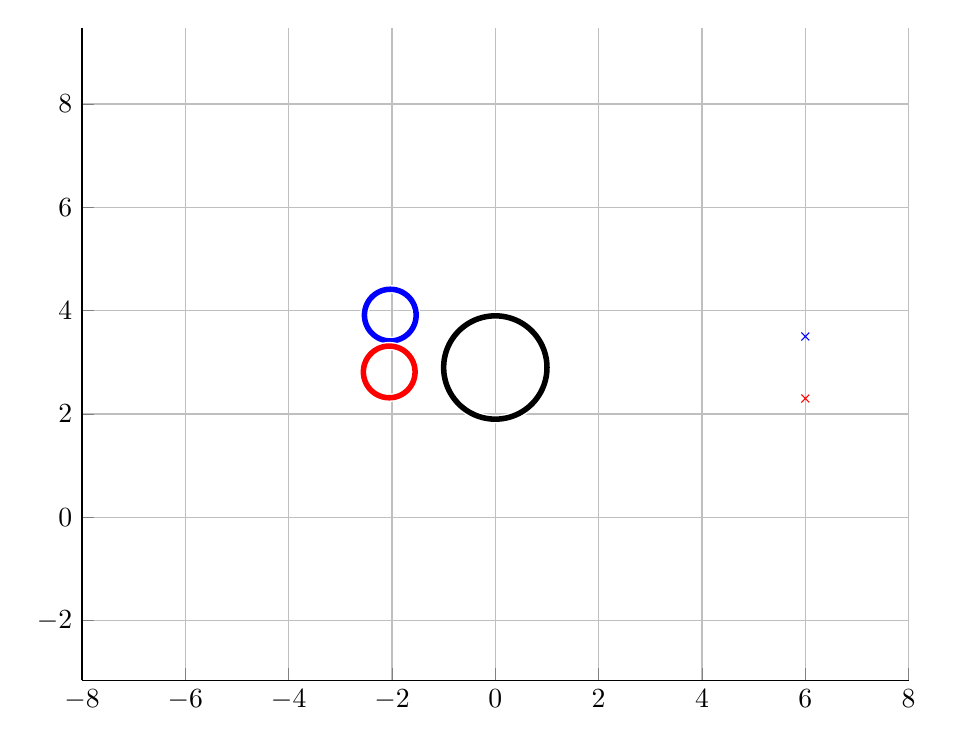
\begin{tikzpicture}

\begin{axis}[%
width=4.133in,
height=3.26in,
at={(0.693in,0.44in)},
scale only axis,
unbounded coords=jump,
xmin=-8,
xmax=8,
xmajorgrids,
ymin=-3.15249042619124,
ymax=9.46686441251843,
ymajorgrids,
axis background/.style={fill=white},
axis x line*=bottom,
axis y line*=left
]
\addplot [color=blue,only marks,mark=x,mark options={solid},forget plot]
  table[row sep=crcr]{%
6	3.5\\
};
\addplot [color=red,only marks,mark=x,mark options={solid},forget plot]
  table[row sep=crcr]{%
6	2.3\\
};
\addplot [color=white,solid,line width=3.0pt,forget plot]
  table[row sep=crcr]{%
-1.53306914168459	3.91437398632719\\
-1.53337372817504	3.93182373467844\\
-1.53428711655468	3.94925222319925\\
-1.53580819400045	3.96663821796101\\
-1.5379351073138	3.98396053680722\\
-1.54066526517848	4.00119807516065\\
-1.54399534131769	4.01832983173607\\
-1.54792127854659	4.03533493412702\\
-1.55243829371543	4.05219266423569\\
-1.55754088353701	4.06888248351466\\
-1.56322283129163	4.08538405799002\\
-1.5694772144012	4.10167728303514\\
-1.57629641286329	4.11774230786509\\
-1.58367211853501	4.13355955972172\\
-1.59159534525513	4.14910976772013\\
-1.60005643979237	4.16437398632719\\
-1.60904509360638	4.17933361844379\\
-1.61855035540707	4.19397043806256\\
-1.62856064449712	4.20826661247342\\
-1.63906376488123	4.22220472399002\\
-1.6500469201251	4.23576779117046\\
-1.66149672894589	4.24893928950662\\
-1.67339924151526	4.26170317155669\\
-1.68573995645509	4.27404388649651\\
-1.69850383850516	4.28594639906588\\
-1.71167533684132	4.29739620788668\\
-1.72523840402176	4.30837936313055\\
-1.73917651553835	4.31888248351466\\
-1.75347268994922	4.32889277260471\\
-1.76810950956799	4.3383980344054\\
-1.78306914168459	4.34738668821941\\
-1.79833336029164	4.35584778275665\\
-1.81388356829005	4.36377100947677\\
-1.82970082014669	4.37114671514849\\
-1.84576584497663	4.37796591361058\\
-1.86205907002175	4.38422029672014\\
-1.87856064449712	4.38990224447476\\
-1.89525046377609	4.39500483429635\\
-1.91210819388475	4.39952184946518\\
-1.92911329627571	4.40344778669409\\
-1.94624505285112	4.40677786283329\\
-1.96348259120456	4.40950802069797\\
-1.98080491005076	4.41163493401132\\
-1.99819090481253	4.4131560114571\\
-2.01561939333334	4.41406939983673\\
-2.03306914168459	4.41437398632719\\
-2.05051889003584	4.41406939983673\\
-2.06794737855665	4.4131560114571\\
-2.08533337331842	4.41163493401132\\
-2.10265569216462	4.40950802069797\\
-2.11989323051805	4.40677786283329\\
-2.13702498709347	4.40344778669409\\
-2.15403008948442	4.39952184946518\\
-2.17088781959309	4.39500483429635\\
-2.18757763887206	4.38990224447476\\
-2.20407921334742	4.38422029672014\\
-2.22037243839254	4.37796591361058\\
-2.23643746322249	4.37114671514849\\
-2.25225471507913	4.36377100947677\\
-2.26780492307753	4.35584778275665\\
-2.28306914168459	4.34738668821941\\
-2.29802877380119	4.3383980344054\\
-2.31266559341996	4.32889277260471\\
-2.32696176783083	4.31888248351466\\
-2.34089987934742	4.30837936313055\\
-2.35446294652786	4.29739620788668\\
-2.36763444486402	4.28594639906588\\
-2.38039832691409	4.27404388649651\\
-2.39273904185391	4.26170317155669\\
-2.40464155442329	4.24893928950662\\
-2.41609136324408	4.23576779117046\\
-2.42707451848795	4.22220472399002\\
-2.43757763887206	4.20826661247342\\
-2.44758792796211	4.19397043806256\\
-2.4570931897628	4.17933361844379\\
-2.46608184357681	4.16437398632719\\
-2.47454293811405	4.14910976772013\\
-2.48246616483417	4.13355955972172\\
-2.48984187050589	4.11774230786509\\
-2.49666106896798	4.10167728303514\\
-2.50291545207754	4.08538405799002\\
-2.50859739983217	4.06888248351466\\
-2.51369998965375	4.05219266423569\\
-2.51821700482259	4.03533493412702\\
-2.52214294205149	4.01832983173607\\
-2.52547301819069	4.00119807516065\\
-2.52820317605537	3.98396053680722\\
-2.53033008936873	3.96663821796101\\
-2.5318511668145	3.94925222319925\\
-2.53276455519414	3.93182373467844\\
-2.53306914168459	3.91437398632719\\
-2.53276455519414	3.89692423797594\\
-2.5318511668145	3.87949574945512\\
-2.53033008936873	3.86210975469336\\
-2.52820317605537	3.84478743584715\\
-2.52547301819069	3.82754989749372\\
-2.52214294205149	3.81041814091831\\
-2.51821700482259	3.79341303852735\\
-2.51369998965375	3.77655530841869\\
-2.50859739983217	3.75986548913971\\
-2.50291545207754	3.74336391466435\\
-2.49666106896798	3.72707068961923\\
-2.48984187050589	3.71100566478929\\
-2.48246616483417	3.69518841293265\\
-2.47454293811405	3.67963820493424\\
-2.46608184357681	3.66437398632719\\
-2.4570931897628	3.64941435421058\\
-2.44758792796211	3.63477753459181\\
-2.43757763887206	3.62048136018095\\
-2.42707451848795	3.60654324866436\\
-2.41609136324408	3.59298018148392\\
-2.40464155442329	3.57980868314776\\
-2.39273904185391	3.56704480109769\\
-2.38039832691409	3.55470408615786\\
-2.36763444486402	3.54280157358849\\
-2.35446294652786	3.5313517647677\\
-2.34089987934742	3.52036860952383\\
-2.32696176783083	3.50986548913971\\
-2.31266559341996	3.49985520004967\\
-2.29802877380119	3.49034993824897\\
-2.28306914168459	3.48136128443497\\
-2.26780492307753	3.47290018989772\\
-2.25225471507913	3.4649769631776\\
-2.23643746322249	3.45760125750589\\
-2.22037243839254	3.45078205904379\\
-2.20407921334742	3.44452767593423\\
-2.18757763887206	3.43884572817961\\
-2.17088781959309	3.43374313835803\\
-2.15403008948442	3.42922612318919\\
-2.13702498709347	3.42530018596028\\
-2.11989323051805	3.42197010982108\\
-2.10265569216462	3.4192399519564\\
-2.08533337331842	3.41711303864305\\
-2.06794737855665	3.41559196119727\\
-2.05051889003584	3.41467857281764\\
-2.03306914168459	3.41437398632719\\
-2.01561939333334	3.41467857281764\\
-1.99819090481253	3.41559196119727\\
-1.98080491005076	3.41711303864305\\
-1.96348259120456	3.4192399519564\\
-1.94624505285112	3.42197010982108\\
-1.92911329627571	3.42530018596028\\
-1.91210819388476	3.42922612318919\\
-1.89525046377609	3.43374313835803\\
-1.87856064449712	3.43884572817961\\
-1.86205907002175	3.44452767593423\\
-1.84576584497663	3.45078205904379\\
-1.82970082014669	3.45760125750589\\
-1.81388356829005	3.4649769631776\\
-1.79833336029164	3.47290018989772\\
-1.78306914168459	3.48136128443497\\
-1.76810950956799	3.49034993824897\\
-1.75347268994922	3.49985520004967\\
-1.73917651553835	3.50986548913971\\
-1.72523840402176	3.52036860952383\\
-1.71167533684132	3.5313517647677\\
-1.69850383850516	3.54280157358849\\
-1.68573995645509	3.55470408615786\\
-1.67339924151526	3.56704480109769\\
-1.66149672894589	3.57980868314776\\
-1.6500469201251	3.59298018148392\\
-1.63906376488123	3.60654324866436\\
-1.62856064449712	3.62048136018095\\
-1.61855035540707	3.63477753459181\\
-1.60904509360638	3.64941435421058\\
-1.60005643979237	3.66437398632719\\
-1.59159534525513	3.67963820493424\\
-1.58367211853501	3.69518841293265\\
-1.57629641286329	3.71100566478929\\
-1.5694772144012	3.72707068961923\\
-1.56322283129163	3.74336391466435\\
-1.55754088353701	3.75986548913971\\
-1.55243829371543	3.77655530841869\\
-1.54792127854659	3.79341303852735\\
-1.54399534131769	3.81041814091831\\
-1.54066526517848	3.82754989749372\\
-1.5379351073138	3.84478743584715\\
-1.53580819400045	3.86210975469336\\
-1.53428711655468	3.87949574945512\\
-1.53337372817504	3.89692423797594\\
-1.53306914168459	3.91437398632719\\
nan	nan\\
};
\addplot [color=blue,solid,line width=2.0pt,forget plot]
  table[row sep=crcr]{%
-1.53306914168459	3.91437398632719\\
-1.53337372817504	3.93182373467844\\
-1.53428711655468	3.94925222319925\\
-1.53580819400045	3.96663821796101\\
-1.5379351073138	3.98396053680722\\
-1.54066526517848	4.00119807516065\\
-1.54399534131769	4.01832983173607\\
-1.54792127854659	4.03533493412702\\
-1.55243829371543	4.05219266423569\\
-1.55754088353701	4.06888248351466\\
-1.56322283129163	4.08538405799002\\
-1.5694772144012	4.10167728303514\\
-1.57629641286329	4.11774230786509\\
-1.58367211853501	4.13355955972172\\
-1.59159534525513	4.14910976772013\\
-1.60005643979237	4.16437398632719\\
-1.60904509360638	4.17933361844379\\
-1.61855035540707	4.19397043806256\\
-1.62856064449712	4.20826661247342\\
-1.63906376488123	4.22220472399002\\
-1.6500469201251	4.23576779117046\\
-1.66149672894589	4.24893928950662\\
-1.67339924151526	4.26170317155669\\
-1.68573995645509	4.27404388649651\\
-1.69850383850516	4.28594639906588\\
-1.71167533684132	4.29739620788668\\
-1.72523840402176	4.30837936313055\\
-1.73917651553835	4.31888248351466\\
-1.75347268994922	4.32889277260471\\
-1.76810950956799	4.3383980344054\\
-1.78306914168459	4.34738668821941\\
-1.79833336029164	4.35584778275665\\
-1.81388356829005	4.36377100947677\\
-1.82970082014669	4.37114671514849\\
-1.84576584497663	4.37796591361058\\
-1.86205907002175	4.38422029672014\\
-1.87856064449712	4.38990224447476\\
-1.89525046377609	4.39500483429635\\
-1.91210819388475	4.39952184946518\\
-1.92911329627571	4.40344778669409\\
-1.94624505285112	4.40677786283329\\
-1.96348259120456	4.40950802069797\\
-1.98080491005076	4.41163493401132\\
-1.99819090481253	4.4131560114571\\
-2.01561939333334	4.41406939983673\\
-2.03306914168459	4.41437398632719\\
-2.05051889003584	4.41406939983673\\
-2.06794737855665	4.4131560114571\\
-2.08533337331842	4.41163493401132\\
-2.10265569216462	4.40950802069797\\
-2.11989323051805	4.40677786283329\\
-2.13702498709347	4.40344778669409\\
-2.15403008948442	4.39952184946518\\
-2.17088781959309	4.39500483429635\\
-2.18757763887206	4.38990224447476\\
-2.20407921334742	4.38422029672014\\
-2.22037243839254	4.37796591361058\\
-2.23643746322249	4.37114671514849\\
-2.25225471507913	4.36377100947677\\
-2.26780492307753	4.35584778275665\\
-2.28306914168459	4.34738668821941\\
-2.29802877380119	4.3383980344054\\
-2.31266559341996	4.32889277260471\\
-2.32696176783083	4.31888248351466\\
-2.34089987934742	4.30837936313055\\
-2.35446294652786	4.29739620788668\\
-2.36763444486402	4.28594639906588\\
-2.38039832691409	4.27404388649651\\
-2.39273904185391	4.26170317155669\\
-2.40464155442329	4.24893928950662\\
-2.41609136324408	4.23576779117046\\
-2.42707451848795	4.22220472399002\\
-2.43757763887206	4.20826661247342\\
-2.44758792796211	4.19397043806256\\
-2.4570931897628	4.17933361844379\\
-2.46608184357681	4.16437398632719\\
-2.47454293811405	4.14910976772013\\
-2.48246616483417	4.13355955972172\\
-2.48984187050589	4.11774230786509\\
-2.49666106896798	4.10167728303514\\
-2.50291545207754	4.08538405799002\\
-2.50859739983217	4.06888248351466\\
-2.51369998965375	4.05219266423569\\
-2.51821700482259	4.03533493412702\\
-2.52214294205149	4.01832983173607\\
-2.52547301819069	4.00119807516065\\
-2.52820317605537	3.98396053680722\\
-2.53033008936873	3.96663821796101\\
-2.5318511668145	3.94925222319925\\
-2.53276455519414	3.93182373467844\\
-2.53306914168459	3.91437398632719\\
-2.53276455519414	3.89692423797594\\
-2.5318511668145	3.87949574945512\\
-2.53033008936873	3.86210975469336\\
-2.52820317605537	3.84478743584715\\
-2.52547301819069	3.82754989749372\\
-2.52214294205149	3.81041814091831\\
-2.51821700482259	3.79341303852735\\
-2.51369998965375	3.77655530841869\\
-2.50859739983217	3.75986548913971\\
-2.50291545207754	3.74336391466435\\
-2.49666106896798	3.72707068961923\\
-2.48984187050589	3.71100566478929\\
-2.48246616483417	3.69518841293265\\
-2.47454293811405	3.67963820493424\\
-2.46608184357681	3.66437398632719\\
-2.4570931897628	3.64941435421058\\
-2.44758792796211	3.63477753459181\\
-2.43757763887206	3.62048136018095\\
-2.42707451848795	3.60654324866436\\
-2.41609136324408	3.59298018148392\\
-2.40464155442329	3.57980868314776\\
-2.39273904185391	3.56704480109769\\
-2.38039832691409	3.55470408615786\\
-2.36763444486402	3.54280157358849\\
-2.35446294652786	3.5313517647677\\
-2.34089987934742	3.52036860952383\\
-2.32696176783083	3.50986548913971\\
-2.31266559341996	3.49985520004967\\
-2.29802877380119	3.49034993824897\\
-2.28306914168459	3.48136128443497\\
-2.26780492307753	3.47290018989772\\
-2.25225471507913	3.4649769631776\\
-2.23643746322249	3.45760125750589\\
-2.22037243839254	3.45078205904379\\
-2.20407921334742	3.44452767593423\\
-2.18757763887206	3.43884572817961\\
-2.17088781959309	3.43374313835803\\
-2.15403008948442	3.42922612318919\\
-2.13702498709347	3.42530018596028\\
-2.11989323051805	3.42197010982108\\
-2.10265569216462	3.4192399519564\\
-2.08533337331842	3.41711303864305\\
-2.06794737855665	3.41559196119727\\
-2.05051889003584	3.41467857281764\\
-2.03306914168459	3.41437398632719\\
-2.01561939333334	3.41467857281764\\
-1.99819090481253	3.41559196119727\\
-1.98080491005076	3.41711303864305\\
-1.96348259120456	3.4192399519564\\
-1.94624505285112	3.42197010982108\\
-1.92911329627571	3.42530018596028\\
-1.91210819388476	3.42922612318919\\
-1.89525046377609	3.43374313835803\\
-1.87856064449712	3.43884572817961\\
-1.86205907002175	3.44452767593423\\
-1.84576584497663	3.45078205904379\\
-1.82970082014669	3.45760125750589\\
-1.81388356829005	3.4649769631776\\
-1.79833336029164	3.47290018989772\\
-1.78306914168459	3.48136128443497\\
-1.76810950956799	3.49034993824897\\
-1.75347268994922	3.49985520004967\\
-1.73917651553835	3.50986548913971\\
-1.72523840402176	3.52036860952383\\
-1.71167533684132	3.5313517647677\\
-1.69850383850516	3.54280157358849\\
-1.68573995645509	3.55470408615786\\
-1.67339924151526	3.56704480109769\\
-1.66149672894589	3.57980868314776\\
-1.6500469201251	3.59298018148392\\
-1.63906376488123	3.60654324866436\\
-1.62856064449712	3.62048136018095\\
-1.61855035540707	3.63477753459181\\
-1.60904509360638	3.64941435421058\\
-1.60005643979237	3.66437398632719\\
-1.59159534525513	3.67963820493424\\
-1.58367211853501	3.69518841293265\\
-1.57629641286329	3.71100566478929\\
-1.5694772144012	3.72707068961923\\
-1.56322283129163	3.74336391466435\\
-1.55754088353701	3.75986548913971\\
-1.55243829371543	3.77655530841869\\
-1.54792127854659	3.79341303852735\\
-1.54399534131769	3.81041814091831\\
-1.54066526517848	3.82754989749372\\
-1.5379351073138	3.84478743584715\\
-1.53580819400045	3.86210975469336\\
-1.53428711655468	3.87949574945512\\
-1.53337372817504	3.89692423797594\\
-1.53306914168459	3.91437398632719\\
nan	nan\\
};
\addplot [color=white,solid,line width=3.0pt,forget plot]
  table[row sep=crcr]{%
-1.55373409775359	2.81456811273374\\
-1.55403868424404	2.83201786108499\\
-1.55495207262367	2.8494463496058\\
-1.55647315006945	2.86683234436757\\
-1.5586000633828	2.88415466321377\\
-1.56133022124748	2.9013922015672\\
-1.56466029738668	2.91852395814262\\
-1.56858623461559	2.93552906053357\\
-1.57310324978443	2.95238679064224\\
-1.57820583960601	2.96907660992121\\
-1.58388778736063	2.98557818439657\\
-1.59014217047019	3.0018714094417\\
-1.59696136893228	3.01793643427164\\
-1.604337074604	3.03375368612828\\
-1.61226030132412	3.04930389412668\\
-1.62072139586137	3.06456811273374\\
-1.62971004967537	3.07952774485034\\
-1.63921531147606	3.09416456446911\\
-1.64922560056611	3.10846073887998\\
-1.65972872095022	3.12239885039657\\
-1.6707118761941	3.13596191757701\\
-1.68216168501489	3.14913341591317\\
-1.69406419758426	3.16189729796324\\
-1.70640491252409	3.17423801290306\\
-1.71916879457416	3.18614052547244\\
-1.73234029291032	3.19759033429323\\
-1.74590336009076	3.2085734895371\\
-1.75984147160735	3.21907660992121\\
-1.77413764601821	3.22908689901126\\
-1.78877446563698	3.23859216081195\\
-1.80373409775359	3.24758081462596\\
-1.81899831636064	3.2560419091632\\
-1.83454852435905	3.26396513588332\\
-1.85036577621569	3.27134084155504\\
-1.86643080104563	3.27816004001713\\
-1.88272402609075	3.28441442312669\\
-1.89922560056611	3.29009637088132\\
-1.91591541984509	3.2951989607029\\
-1.93277314995375	3.29971597587174\\
-1.94977825234471	3.30364191310064\\
-1.96691000892012	3.30697198923984\\
-1.98414754727355	3.30970214710452\\
-2.00146986611976	3.31182906041788\\
-2.01885586088152	3.31335013786365\\
-2.03628434940233	3.31426352624329\\
-2.05373409775359	3.31456811273374\\
-2.07118384610484	3.31426352624329\\
-2.08861233462565	3.31335013786365\\
-2.10599832938741	3.31182906041788\\
-2.12332064823362	3.30970214710452\\
-2.14055818658705	3.30697198923984\\
-2.15768994316246	3.30364191310064\\
-2.17469504555342	3.29971597587174\\
-2.19155277566208	3.2951989607029\\
-2.20824259494106	3.29009637088132\\
-2.22474416941642	3.28441442312669\\
-2.24103739446154	3.27816004001713\\
-2.25710241929149	3.27134084155504\\
-2.27291967114812	3.26396513588332\\
-2.28846987914653	3.2560419091632\\
-2.30373409775359	3.24758081462596\\
-2.31869372987019	3.23859216081195\\
-2.33333054948896	3.22908689901126\\
-2.34762672389982	3.21907660992121\\
-2.36156483541641	3.2085734895371\\
-2.37512790259686	3.19759033429323\\
-2.38829940093301	3.18614052547244\\
-2.40106328298308	3.17423801290306\\
-2.41340399792291	3.16189729796324\\
-2.42530651049228	3.14913341591317\\
-2.43675631931307	3.13596191757701\\
-2.44773947455695	3.12239885039657\\
-2.45824259494106	3.10846073887998\\
-2.46825288403111	3.09416456446911\\
-2.4777581458318	3.07952774485034\\
-2.4867467996458	3.06456811273374\\
-2.49520789418305	3.04930389412668\\
-2.50313112090317	3.03375368612828\\
-2.51050682657489	3.01793643427164\\
-2.51732602503698	3.0018714094417\\
-2.52358040814654	2.98557818439657\\
-2.52926235590116	2.96907660992121\\
-2.53436494572274	2.95238679064224\\
-2.53888196089158	2.93552906053357\\
-2.54280789812049	2.91852395814262\\
-2.54613797425969	2.9013922015672\\
-2.54886813212437	2.88415466321377\\
-2.55099504543772	2.86683234436757\\
-2.5525161228835	2.8494463496058\\
-2.55342951126313	2.83201786108499\\
-2.55373409775359	2.81456811273374\\
-2.55342951126313	2.79711836438249\\
-2.5525161228835	2.77968987586168\\
-2.55099504543772	2.76230388109991\\
-2.54886813212437	2.74498156225371\\
-2.54613797425969	2.72774402390027\\
-2.54280789812049	2.71061226732486\\
-2.53888196089158	2.69360716493391\\
-2.53436494572274	2.67674943482524\\
-2.52926235590116	2.66005961554627\\
-2.52358040814654	2.6435580410709\\
-2.51732602503698	2.62726481602578\\
-2.51050682657489	2.61119979119584\\
-2.50313112090317	2.5953825393392\\
-2.49520789418305	2.57983233134079\\
-2.4867467996458	2.56456811273374\\
-2.4777581458318	2.54960848061714\\
-2.46825288403111	2.53497166099837\\
-2.45824259494106	2.5206754865875\\
-2.44773947455695	2.50673737507091\\
-2.43675631931307	2.49317430789047\\
-2.42530651049228	2.48000280955431\\
-2.41340399792291	2.46723892750424\\
-2.40106328298308	2.45489821256441\\
-2.38829940093301	2.44299569999504\\
-2.37512790259686	2.43154589117425\\
-2.36156483541641	2.42056273593038\\
-2.34762672389982	2.41005961554627\\
-2.33333054948896	2.40004932645622\\
-2.31869372987019	2.39054406465553\\
-2.30373409775359	2.38155541084152\\
-2.28846987914653	2.37309431630428\\
-2.27291967114812	2.36517108958416\\
-2.25710241929149	2.35779538391244\\
-2.24103739446154	2.35097618545035\\
-2.22474416941642	2.34472180234079\\
-2.20824259494106	2.33903985458616\\
-2.19155277566208	2.33393726476458\\
-2.17469504555342	2.32942024959574\\
-2.15768994316246	2.32549431236684\\
-2.14055818658705	2.32216423622764\\
-2.12332064823362	2.31943407836295\\
-2.10599832938741	2.3173071650496\\
-2.08861233462565	2.31578608760383\\
-2.07118384610484	2.31487269922419\\
-2.05373409775359	2.31456811273374\\
-2.03628434940233	2.31487269922419\\
-2.01885586088152	2.31578608760383\\
-2.00146986611976	2.3173071650496\\
-1.98414754727355	2.31943407836295\\
-1.96691000892012	2.32216423622764\\
-1.94977825234471	2.32549431236684\\
-1.93277314995375	2.32942024959574\\
-1.91591541984509	2.33393726476458\\
-1.89922560056611	2.33903985458616\\
-1.88272402609075	2.34472180234078\\
-1.86643080104563	2.35097618545035\\
-1.85036577621568	2.35779538391244\\
-1.83454852435905	2.36517108958416\\
-1.81899831636064	2.37309431630428\\
-1.80373409775359	2.38155541084152\\
-1.78877446563698	2.39054406465553\\
-1.77413764601821	2.40004932645622\\
-1.75984147160735	2.41005961554627\\
-1.74590336009076	2.42056273593038\\
-1.73234029291032	2.43154589117425\\
-1.71916879457416	2.44299569999504\\
-1.70640491252409	2.45489821256441\\
-1.69406419758426	2.46723892750424\\
-1.68216168501489	2.48000280955431\\
-1.6707118761941	2.49317430789047\\
-1.65972872095022	2.50673737507091\\
-1.64922560056611	2.5206754865875\\
-1.63921531147606	2.53497166099837\\
-1.62971004967537	2.54960848061714\\
-1.62072139586137	2.56456811273374\\
-1.61226030132412	2.57983233134079\\
-1.604337074604	2.5953825393392\\
-1.59696136893228	2.61119979119584\\
-1.59014217047019	2.62726481602578\\
-1.58388778736063	2.6435580410709\\
-1.57820583960601	2.66005961554627\\
-1.57310324978443	2.67674943482524\\
-1.56858623461559	2.69360716493391\\
-1.56466029738668	2.71061226732486\\
-1.56133022124748	2.72774402390027\\
-1.5586000633828	2.74498156225371\\
-1.55647315006945	2.76230388109991\\
-1.55495207262367	2.77968987586168\\
-1.55403868424404	2.79711836438249\\
-1.55373409775359	2.81456811273374\\
nan	nan\\
};
\addplot [color=red,solid,line width=2.0pt,forget plot]
  table[row sep=crcr]{%
-1.55373409775359	2.81456811273374\\
-1.55403868424404	2.83201786108499\\
-1.55495207262367	2.8494463496058\\
-1.55647315006945	2.86683234436757\\
-1.5586000633828	2.88415466321377\\
-1.56133022124748	2.9013922015672\\
-1.56466029738668	2.91852395814262\\
-1.56858623461559	2.93552906053357\\
-1.57310324978443	2.95238679064224\\
-1.57820583960601	2.96907660992121\\
-1.58388778736063	2.98557818439657\\
-1.59014217047019	3.0018714094417\\
-1.59696136893228	3.01793643427164\\
-1.604337074604	3.03375368612828\\
-1.61226030132412	3.04930389412668\\
-1.62072139586137	3.06456811273374\\
-1.62971004967537	3.07952774485034\\
-1.63921531147606	3.09416456446911\\
-1.64922560056611	3.10846073887998\\
-1.65972872095022	3.12239885039657\\
-1.6707118761941	3.13596191757701\\
-1.68216168501489	3.14913341591317\\
-1.69406419758426	3.16189729796324\\
-1.70640491252409	3.17423801290306\\
-1.71916879457416	3.18614052547244\\
-1.73234029291032	3.19759033429323\\
-1.74590336009076	3.2085734895371\\
-1.75984147160735	3.21907660992121\\
-1.77413764601821	3.22908689901126\\
-1.78877446563698	3.23859216081195\\
-1.80373409775359	3.24758081462596\\
-1.81899831636064	3.2560419091632\\
-1.83454852435905	3.26396513588332\\
-1.85036577621569	3.27134084155504\\
-1.86643080104563	3.27816004001713\\
-1.88272402609075	3.28441442312669\\
-1.89922560056611	3.29009637088132\\
-1.91591541984509	3.2951989607029\\
-1.93277314995375	3.29971597587174\\
-1.94977825234471	3.30364191310064\\
-1.96691000892012	3.30697198923984\\
-1.98414754727355	3.30970214710452\\
-2.00146986611976	3.31182906041788\\
-2.01885586088152	3.31335013786365\\
-2.03628434940233	3.31426352624329\\
-2.05373409775359	3.31456811273374\\
-2.07118384610484	3.31426352624329\\
-2.08861233462565	3.31335013786365\\
-2.10599832938741	3.31182906041788\\
-2.12332064823362	3.30970214710452\\
-2.14055818658705	3.30697198923984\\
-2.15768994316246	3.30364191310064\\
-2.17469504555342	3.29971597587174\\
-2.19155277566208	3.2951989607029\\
-2.20824259494106	3.29009637088132\\
-2.22474416941642	3.28441442312669\\
-2.24103739446154	3.27816004001713\\
-2.25710241929149	3.27134084155504\\
-2.27291967114812	3.26396513588332\\
-2.28846987914653	3.2560419091632\\
-2.30373409775359	3.24758081462596\\
-2.31869372987019	3.23859216081195\\
-2.33333054948896	3.22908689901126\\
-2.34762672389982	3.21907660992121\\
-2.36156483541641	3.2085734895371\\
-2.37512790259686	3.19759033429323\\
-2.38829940093301	3.18614052547244\\
-2.40106328298308	3.17423801290306\\
-2.41340399792291	3.16189729796324\\
-2.42530651049228	3.14913341591317\\
-2.43675631931307	3.13596191757701\\
-2.44773947455695	3.12239885039657\\
-2.45824259494106	3.10846073887998\\
-2.46825288403111	3.09416456446911\\
-2.4777581458318	3.07952774485034\\
-2.4867467996458	3.06456811273374\\
-2.49520789418305	3.04930389412668\\
-2.50313112090317	3.03375368612828\\
-2.51050682657489	3.01793643427164\\
-2.51732602503698	3.0018714094417\\
-2.52358040814654	2.98557818439657\\
-2.52926235590116	2.96907660992121\\
-2.53436494572274	2.95238679064224\\
-2.53888196089158	2.93552906053357\\
-2.54280789812049	2.91852395814262\\
-2.54613797425969	2.9013922015672\\
-2.54886813212437	2.88415466321377\\
-2.55099504543772	2.86683234436757\\
-2.5525161228835	2.8494463496058\\
-2.55342951126313	2.83201786108499\\
-2.55373409775359	2.81456811273374\\
-2.55342951126313	2.79711836438249\\
-2.5525161228835	2.77968987586168\\
-2.55099504543772	2.76230388109991\\
-2.54886813212437	2.74498156225371\\
-2.54613797425969	2.72774402390027\\
-2.54280789812049	2.71061226732486\\
-2.53888196089158	2.69360716493391\\
-2.53436494572274	2.67674943482524\\
-2.52926235590116	2.66005961554627\\
-2.52358040814654	2.6435580410709\\
-2.51732602503698	2.62726481602578\\
-2.51050682657489	2.61119979119584\\
-2.50313112090317	2.5953825393392\\
-2.49520789418305	2.57983233134079\\
-2.4867467996458	2.56456811273374\\
-2.4777581458318	2.54960848061714\\
-2.46825288403111	2.53497166099837\\
-2.45824259494106	2.5206754865875\\
-2.44773947455695	2.50673737507091\\
-2.43675631931307	2.49317430789047\\
-2.42530651049228	2.48000280955431\\
-2.41340399792291	2.46723892750424\\
-2.40106328298308	2.45489821256441\\
-2.38829940093301	2.44299569999504\\
-2.37512790259686	2.43154589117425\\
-2.36156483541641	2.42056273593038\\
-2.34762672389982	2.41005961554627\\
-2.33333054948896	2.40004932645622\\
-2.31869372987019	2.39054406465553\\
-2.30373409775359	2.38155541084152\\
-2.28846987914653	2.37309431630428\\
-2.27291967114812	2.36517108958416\\
-2.25710241929149	2.35779538391244\\
-2.24103739446154	2.35097618545035\\
-2.22474416941642	2.34472180234079\\
-2.20824259494106	2.33903985458616\\
-2.19155277566208	2.33393726476458\\
-2.17469504555342	2.32942024959574\\
-2.15768994316246	2.32549431236684\\
-2.14055818658705	2.32216423622764\\
-2.12332064823362	2.31943407836295\\
-2.10599832938741	2.3173071650496\\
-2.08861233462565	2.31578608760383\\
-2.07118384610484	2.31487269922419\\
-2.05373409775359	2.31456811273374\\
-2.03628434940233	2.31487269922419\\
-2.01885586088152	2.31578608760383\\
-2.00146986611976	2.3173071650496\\
-1.98414754727355	2.31943407836295\\
-1.96691000892012	2.32216423622764\\
-1.94977825234471	2.32549431236684\\
-1.93277314995375	2.32942024959574\\
-1.91591541984509	2.33393726476458\\
-1.89922560056611	2.33903985458616\\
-1.88272402609075	2.34472180234078\\
-1.86643080104563	2.35097618545035\\
-1.85036577621568	2.35779538391244\\
-1.83454852435905	2.36517108958416\\
-1.81899831636064	2.37309431630428\\
-1.80373409775359	2.38155541084152\\
-1.78877446563698	2.39054406465553\\
-1.77413764601821	2.40004932645622\\
-1.75984147160735	2.41005961554627\\
-1.74590336009076	2.42056273593038\\
-1.73234029291032	2.43154589117425\\
-1.71916879457416	2.44299569999504\\
-1.70640491252409	2.45489821256441\\
-1.69406419758426	2.46723892750424\\
-1.68216168501489	2.48000280955431\\
-1.6707118761941	2.49317430789047\\
-1.65972872095022	2.50673737507091\\
-1.64922560056611	2.5206754865875\\
-1.63921531147606	2.53497166099837\\
-1.62971004967537	2.54960848061714\\
-1.62072139586137	2.56456811273374\\
-1.61226030132412	2.57983233134079\\
-1.604337074604	2.5953825393392\\
-1.59696136893228	2.61119979119584\\
-1.59014217047019	2.62726481602578\\
-1.58388778736063	2.6435580410709\\
-1.57820583960601	2.66005961554627\\
-1.57310324978443	2.67674943482524\\
-1.56858623461559	2.69360716493391\\
-1.56466029738668	2.71061226732486\\
-1.56133022124748	2.72774402390027\\
-1.5586000633828	2.74498156225371\\
-1.55647315006945	2.76230388109991\\
-1.55495207262367	2.77968987586168\\
-1.55403868424404	2.79711836438249\\
-1.55373409775359	2.81456811273374\\
nan	nan\\
};
\addplot [color=white,solid,line width=3.0pt,forget plot]
  table[row sep=crcr]{%
1	2.9\\
0.999390827019096	2.9348994967025\\
0.997564050259824	2.96975647374413\\
0.994521895368273	3.00452846326765\\
0.99026806874157	3.03917310096007\\
0.984807753012208	3.07364817766693\\
0.978147600733806	3.10791169081776\\
0.970295726275996	3.14192189559967\\
0.961261695938319	3.175637355817\\
0.951056516295154	3.20901699437495\\
0.939692620785908	3.24202014332567\\
0.927183854566787	3.27460659341591\\
0.913545457642601	3.3067366430758\\
0.898794046299167	3.33837114678908\\
0.882947592858927	3.36947156278589\\
0.866025403784439	3.4\\
0.848048096156426	3.42991926423321\\
0.829037572555042	3.45919290347075\\
0.809016994374947	3.48778525229247\\
0.788010753606722	3.51566147532566\\
0.766044443118978	3.54278760968654\\
0.743144825477394	3.56913060635886\\
0.719339800338651	3.594658370459\\
0.694658370458997	3.61933980033865\\
0.669130606358858	3.64314482547739\\
0.642787609686539	3.66604444311898\\
0.615661475325658	3.68801075360672\\
0.587785252292473	3.70901699437495\\
0.559192903470747	3.72903757255504\\
0.529919264233205	3.74804809615643\\
0.5	3.76602540378444\\
0.469471562785891	3.78294759285893\\
0.438371146789077	3.79879404629917\\
0.4067366430758	3.8135454576426\\
0.374606593415912	3.82718385456679\\
0.342020143325669	3.83969262078591\\
0.309016994374947	3.85105651629515\\
0.275637355816999	3.86126169593832\\
0.241921895599668	3.870295726276\\
0.207911690817759	3.87814760073381\\
0.17364817766693	3.88480775301221\\
0.139173100960066	3.89026806874157\\
0.104528463267653	3.89452189536827\\
0.0697564737441255	3.89756405025982\\
0.0348994967025011	3.8993908270191\\
6.12323399573677e-17	3.9\\
-0.0348994967025007	3.8993908270191\\
-0.0697564737441253	3.89756405025982\\
-0.104528463267653	3.89452189536827\\
-0.139173100960065	3.89026806874157\\
-0.17364817766693	3.88480775301221\\
-0.207911690817759	3.87814760073381\\
-0.241921895599668	3.870295726276\\
-0.275637355816999	3.86126169593832\\
-0.309016994374947	3.85105651629515\\
-0.342020143325669	3.83969262078591\\
-0.374606593415912	3.82718385456679\\
-0.4067366430758	3.8135454576426\\
-0.438371146789078	3.79879404629917\\
-0.469471562785891	3.78294759285893\\
-0.5	3.76602540378444\\
-0.529919264233205	3.74804809615643\\
-0.559192903470747	3.72903757255504\\
-0.587785252292473	3.70901699437495\\
-0.615661475325658	3.68801075360672\\
-0.642787609686539	3.66604444311898\\
-0.669130606358858	3.64314482547739\\
-0.694658370458997	3.61933980033865\\
-0.719339800338651	3.594658370459\\
-0.743144825477394	3.56913060635886\\
-0.766044443118978	3.54278760968654\\
-0.788010753606722	3.51566147532566\\
-0.809016994374947	3.48778525229247\\
-0.829037572555042	3.45919290347075\\
-0.848048096156426	3.42991926423321\\
-0.866025403784439	3.4\\
-0.882947592858927	3.36947156278589\\
-0.898794046299167	3.33837114678908\\
-0.913545457642601	3.3067366430758\\
-0.927183854566787	3.27460659341591\\
-0.939692620785908	3.24202014332567\\
-0.951056516295154	3.20901699437495\\
-0.961261695938319	3.175637355817\\
-0.970295726275996	3.14192189559967\\
-0.978147600733806	3.10791169081776\\
-0.984807753012208	3.07364817766693\\
-0.99026806874157	3.03917310096007\\
-0.994521895368273	3.00452846326765\\
-0.997564050259824	2.96975647374413\\
-0.999390827019096	2.9348994967025\\
-1	2.9\\
-0.999390827019096	2.8651005032975\\
-0.997564050259824	2.83024352625588\\
-0.994521895368273	2.79547153673235\\
-0.99026806874157	2.76082689903993\\
-0.984807753012208	2.72635182233307\\
-0.978147600733806	2.69208830918224\\
-0.970295726275997	2.65807810440033\\
-0.961261695938319	2.624362644183\\
-0.951056516295154	2.59098300562505\\
-0.939692620785908	2.55797985667433\\
-0.927183854566787	2.52539340658409\\
-0.913545457642601	2.4932633569242\\
-0.898794046299167	2.46162885321092\\
-0.882947592858927	2.43052843721411\\
-0.866025403784439	2.4\\
-0.848048096156426	2.3700807357668\\
-0.829037572555042	2.34080709652925\\
-0.809016994374947	2.31221474770753\\
-0.788010753606722	2.28433852467434\\
-0.766044443118978	2.25721239031346\\
-0.743144825477394	2.23086939364114\\
-0.719339800338651	2.205341629541\\
-0.694658370458997	2.18066019966135\\
-0.669130606358858	2.15685517452261\\
-0.642787609686539	2.13395555688102\\
-0.615661475325658	2.11198924639328\\
-0.587785252292473	2.09098300562505\\
-0.559192903470747	2.07096242744496\\
-0.529919264233205	2.05195190384357\\
-0.5	2.03397459621556\\
-0.469471562785891	2.01705240714107\\
-0.438371146789078	2.00120595370083\\
-0.4067366430758	1.9864545423574\\
-0.374606593415912	1.97281614543321\\
-0.342020143325669	1.96030737921409\\
-0.309016994374948	1.94894348370485\\
-0.275637355816999	1.93873830406168\\
-0.241921895599668	1.929704273724\\
-0.20791169081776	1.92185239926619\\
-0.17364817766693	1.91519224698779\\
-0.139173100960065	1.90973193125843\\
-0.104528463267653	1.90547810463173\\
-0.0697564737441256	1.90243594974018\\
-0.0348994967025016	1.9006091729809\\
-1.83697019872103e-16	1.9\\
0.0348994967025013	1.9006091729809\\
0.0697564737441252	1.90243594974018\\
0.104528463267653	1.90547810463173\\
0.139173100960065	1.90973193125843\\
0.17364817766693	1.91519224698779\\
0.207911690817759	1.92185239926619\\
0.241921895599667	1.929704273724\\
0.275637355816999	1.93873830406168\\
0.309016994374947	1.94894348370485\\
0.342020143325668	1.96030737921409\\
0.374606593415912	1.97281614543321\\
0.406736643075801	1.9864545423574\\
0.438371146789077	2.00120595370083\\
0.46947156278589	2.01705240714107\\
0.5	2.03397459621556\\
0.529919264233205	2.05195190384357\\
0.559192903470746	2.07096242744496\\
0.587785252292473	2.09098300562505\\
0.615661475325659	2.11198924639328\\
0.642787609686539	2.13395555688102\\
0.669130606358858	2.15685517452261\\
0.694658370458997	2.18066019966135\\
0.719339800338651	2.205341629541\\
0.743144825477394	2.23086939364114\\
0.766044443118978	2.25721239031346\\
0.788010753606722	2.28433852467434\\
0.809016994374947	2.31221474770753\\
0.829037572555041	2.34080709652925\\
0.848048096156425	2.37008073576679\\
0.866025403784438	2.4\\
0.882947592858927	2.43052843721411\\
0.898794046299167	2.46162885321092\\
0.913545457642601	2.4932633569242\\
0.927183854566787	2.52539340658409\\
0.939692620785908	2.55797985667433\\
0.951056516295154	2.59098300562505\\
0.961261695938319	2.624362644183\\
0.970295726275996	2.65807810440033\\
0.978147600733806	2.69208830918224\\
0.984807753012208	2.72635182233307\\
0.99026806874157	2.76082689903993\\
0.994521895368273	2.79547153673235\\
0.997564050259824	2.83024352625588\\
0.999390827019096	2.8651005032975\\
1	2.9\\
nan	nan\\
};
\addplot [color=black,solid,line width=2.0pt,forget plot]
  table[row sep=crcr]{%
1	2.9\\
0.999390827019096	2.9348994967025\\
0.997564050259824	2.96975647374413\\
0.994521895368273	3.00452846326765\\
0.99026806874157	3.03917310096007\\
0.984807753012208	3.07364817766693\\
0.978147600733806	3.10791169081776\\
0.970295726275996	3.14192189559967\\
0.961261695938319	3.175637355817\\
0.951056516295154	3.20901699437495\\
0.939692620785908	3.24202014332567\\
0.927183854566787	3.27460659341591\\
0.913545457642601	3.3067366430758\\
0.898794046299167	3.33837114678908\\
0.882947592858927	3.36947156278589\\
0.866025403784439	3.4\\
0.848048096156426	3.42991926423321\\
0.829037572555042	3.45919290347075\\
0.809016994374947	3.48778525229247\\
0.788010753606722	3.51566147532566\\
0.766044443118978	3.54278760968654\\
0.743144825477394	3.56913060635886\\
0.719339800338651	3.594658370459\\
0.694658370458997	3.61933980033865\\
0.669130606358858	3.64314482547739\\
0.642787609686539	3.66604444311898\\
0.615661475325658	3.68801075360672\\
0.587785252292473	3.70901699437495\\
0.559192903470747	3.72903757255504\\
0.529919264233205	3.74804809615643\\
0.5	3.76602540378444\\
0.469471562785891	3.78294759285893\\
0.438371146789077	3.79879404629917\\
0.4067366430758	3.8135454576426\\
0.374606593415912	3.82718385456679\\
0.342020143325669	3.83969262078591\\
0.309016994374947	3.85105651629515\\
0.275637355816999	3.86126169593832\\
0.241921895599668	3.870295726276\\
0.207911690817759	3.87814760073381\\
0.17364817766693	3.88480775301221\\
0.139173100960066	3.89026806874157\\
0.104528463267653	3.89452189536827\\
0.0697564737441255	3.89756405025982\\
0.0348994967025011	3.8993908270191\\
6.12323399573677e-17	3.9\\
-0.0348994967025007	3.8993908270191\\
-0.0697564737441253	3.89756405025982\\
-0.104528463267653	3.89452189536827\\
-0.139173100960065	3.89026806874157\\
-0.17364817766693	3.88480775301221\\
-0.207911690817759	3.87814760073381\\
-0.241921895599668	3.870295726276\\
-0.275637355816999	3.86126169593832\\
-0.309016994374947	3.85105651629515\\
-0.342020143325669	3.83969262078591\\
-0.374606593415912	3.82718385456679\\
-0.4067366430758	3.8135454576426\\
-0.438371146789078	3.79879404629917\\
-0.469471562785891	3.78294759285893\\
-0.5	3.76602540378444\\
-0.529919264233205	3.74804809615643\\
-0.559192903470747	3.72903757255504\\
-0.587785252292473	3.70901699437495\\
-0.615661475325658	3.68801075360672\\
-0.642787609686539	3.66604444311898\\
-0.669130606358858	3.64314482547739\\
-0.694658370458997	3.61933980033865\\
-0.719339800338651	3.594658370459\\
-0.743144825477394	3.56913060635886\\
-0.766044443118978	3.54278760968654\\
-0.788010753606722	3.51566147532566\\
-0.809016994374947	3.48778525229247\\
-0.829037572555042	3.45919290347075\\
-0.848048096156426	3.42991926423321\\
-0.866025403784439	3.4\\
-0.882947592858927	3.36947156278589\\
-0.898794046299167	3.33837114678908\\
-0.913545457642601	3.3067366430758\\
-0.927183854566787	3.27460659341591\\
-0.939692620785908	3.24202014332567\\
-0.951056516295154	3.20901699437495\\
-0.961261695938319	3.175637355817\\
-0.970295726275996	3.14192189559967\\
-0.978147600733806	3.10791169081776\\
-0.984807753012208	3.07364817766693\\
-0.99026806874157	3.03917310096007\\
-0.994521895368273	3.00452846326765\\
-0.997564050259824	2.96975647374413\\
-0.999390827019096	2.9348994967025\\
-1	2.9\\
-0.999390827019096	2.8651005032975\\
-0.997564050259824	2.83024352625588\\
-0.994521895368273	2.79547153673235\\
-0.99026806874157	2.76082689903993\\
-0.984807753012208	2.72635182233307\\
-0.978147600733806	2.69208830918224\\
-0.970295726275997	2.65807810440033\\
-0.961261695938319	2.624362644183\\
-0.951056516295154	2.59098300562505\\
-0.939692620785908	2.55797985667433\\
-0.927183854566787	2.52539340658409\\
-0.913545457642601	2.4932633569242\\
-0.898794046299167	2.46162885321092\\
-0.882947592858927	2.43052843721411\\
-0.866025403784439	2.4\\
-0.848048096156426	2.3700807357668\\
-0.829037572555042	2.34080709652925\\
-0.809016994374947	2.31221474770753\\
-0.788010753606722	2.28433852467434\\
-0.766044443118978	2.25721239031346\\
-0.743144825477394	2.23086939364114\\
-0.719339800338651	2.205341629541\\
-0.694658370458997	2.18066019966135\\
-0.669130606358858	2.15685517452261\\
-0.642787609686539	2.13395555688102\\
-0.615661475325658	2.11198924639328\\
-0.587785252292473	2.09098300562505\\
-0.559192903470747	2.07096242744496\\
-0.529919264233205	2.05195190384357\\
-0.5	2.03397459621556\\
-0.469471562785891	2.01705240714107\\
-0.438371146789078	2.00120595370083\\
-0.4067366430758	1.9864545423574\\
-0.374606593415912	1.97281614543321\\
-0.342020143325669	1.96030737921409\\
-0.309016994374948	1.94894348370485\\
-0.275637355816999	1.93873830406168\\
-0.241921895599668	1.929704273724\\
-0.20791169081776	1.92185239926619\\
-0.17364817766693	1.91519224698779\\
-0.139173100960065	1.90973193125843\\
-0.104528463267653	1.90547810463173\\
-0.0697564737441256	1.90243594974018\\
-0.0348994967025016	1.9006091729809\\
-1.83697019872103e-16	1.9\\
0.0348994967025013	1.9006091729809\\
0.0697564737441252	1.90243594974018\\
0.104528463267653	1.90547810463173\\
0.139173100960065	1.90973193125843\\
0.17364817766693	1.91519224698779\\
0.207911690817759	1.92185239926619\\
0.241921895599667	1.929704273724\\
0.275637355816999	1.93873830406168\\
0.309016994374947	1.94894348370485\\
0.342020143325668	1.96030737921409\\
0.374606593415912	1.97281614543321\\
0.406736643075801	1.9864545423574\\
0.438371146789077	2.00120595370083\\
0.46947156278589	2.01705240714107\\
0.5	2.03397459621556\\
0.529919264233205	2.05195190384357\\
0.559192903470746	2.07096242744496\\
0.587785252292473	2.09098300562505\\
0.615661475325659	2.11198924639328\\
0.642787609686539	2.13395555688102\\
0.669130606358858	2.15685517452261\\
0.694658370458997	2.18066019966135\\
0.719339800338651	2.205341629541\\
0.743144825477394	2.23086939364114\\
0.766044443118978	2.25721239031346\\
0.788010753606722	2.28433852467434\\
0.809016994374947	2.31221474770753\\
0.829037572555041	2.34080709652925\\
0.848048096156425	2.37008073576679\\
0.866025403784438	2.4\\
0.882947592858927	2.43052843721411\\
0.898794046299167	2.46162885321092\\
0.913545457642601	2.4932633569242\\
0.927183854566787	2.52539340658409\\
0.939692620785908	2.55797985667433\\
0.951056516295154	2.59098300562505\\
0.961261695938319	2.624362644183\\
0.970295726275996	2.65807810440033\\
0.978147600733806	2.69208830918224\\
0.984807753012208	2.72635182233307\\
0.99026806874157	2.76082689903993\\
0.994521895368273	2.79547153673235\\
0.997564050259824	2.83024352625588\\
0.999390827019096	2.8651005032975\\
1	2.9\\
nan	nan\\
};
\end{axis}
\end{tikzpicture}%}
      \caption{}
      \label{}
    \end{figure}
  \end{minipage}
\end{minipage}
}

\noindent\makebox[\linewidth][c]{%
\begin{minipage}{\linewidth}
  \begin{minipage}{0.45\linewidth}
    \begin{figure}[H]
      \scalebox{0.7}{% This file was created by matlab2tikz.
%
%The latest updates can be retrieved from
%  http://www.mathworks.com/matlabcentral/fileexchange/22022-matlab2tikz-matlab2tikz
%where you can also make suggestions and rate matlab2tikz.
%
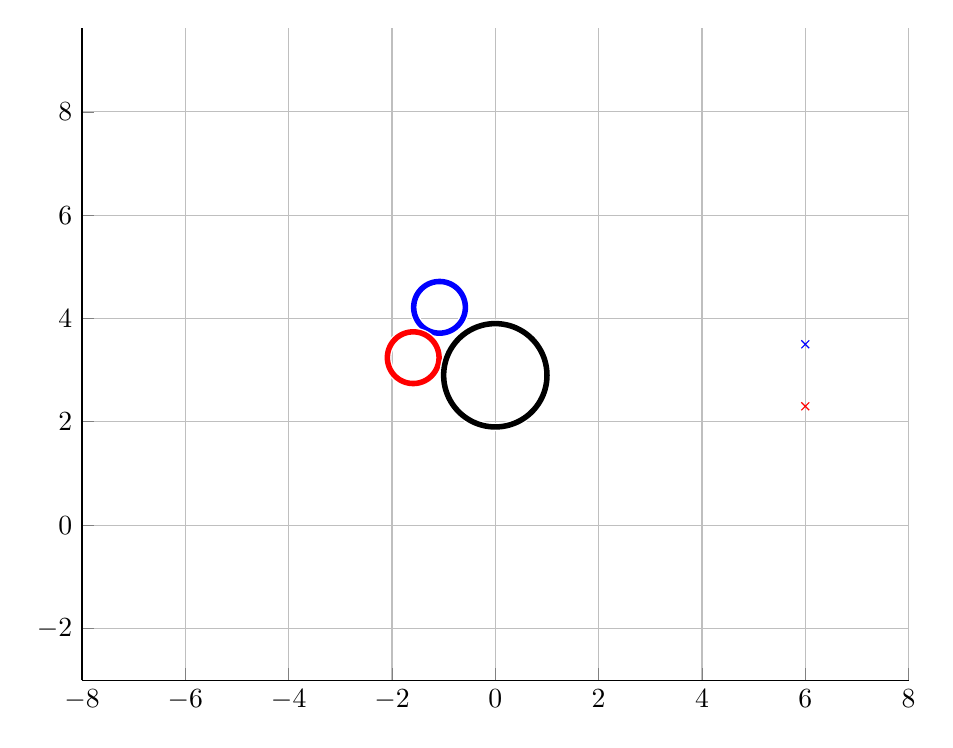
\begin{tikzpicture}

\begin{axis}[%
width=4.133in,
height=3.26in,
at={(0.693in,0.44in)},
scale only axis,
unbounded coords=jump,
xmin=-8,
xmax=8,
xmajorgrids,
ymin=-3.00205312257439,
ymax=9.61730171613528,
ymajorgrids,
axis background/.style={fill=white},
axis x line*=bottom,
axis y line*=left
]
\addplot [color=blue,only marks,mark=x,mark options={solid},forget plot]
  table[row sep=crcr]{%
6	3.5\\
};
\addplot [color=red,only marks,mark=x,mark options={solid},forget plot]
  table[row sep=crcr]{%
6	2.3\\
};
\addplot [color=white,solid,line width=3.0pt,forget plot]
  table[row sep=crcr]{%
-0.580012556236331	4.21524859356089\\
-0.580317142726783	4.23269834191214\\
-0.581230531106419	4.25012683043296\\
-0.582751608552194	4.26751282519472\\
-0.584878521865546	4.28483514404093\\
-0.587608679730227	4.30207268239436\\
-0.590938755869428	4.31920443896977\\
-0.594864693098333	4.33620954136073\\
-0.599381708267171	4.35306727146939\\
-0.604484298088754	4.36975709074837\\
-0.610166245843377	4.38625866522373\\
-0.616420628952937	4.40255189026885\\
-0.62323982741503	4.41861691509879\\
-0.630615533086747	4.43443416695543\\
-0.638538759806867	4.44998437495384\\
-0.646999854344111	4.46524859356089\\
-0.655988508158118	4.4802082256775\\
-0.66549376995881	4.49484504529627\\
-0.675504059048857	4.50914121970713\\
-0.68600717943297	4.52307933122372\\
-0.696990334676842	4.53664239840416\\
-0.708440143497634	4.54981389674032\\
-0.720342656067005	4.56257777879039\\
-0.732683371006832	4.57491849373022\\
-0.745447253056902	4.58682100629959\\
-0.758618751393061	4.59827081512038\\
-0.772181818573502	4.60925397036425\\
-0.786119930090094	4.61975709074837\\
-0.800416104500957	4.62976737983841\\
-0.815052924119728	4.63927264163911\\
-0.830012556236331	4.64826129545311\\
-0.845276774843385	4.65672238999036\\
-0.860826982841792	4.66464561671048\\
-0.876644234698431	4.67202132238219\\
-0.892709259528375	4.67884052084429\\
-0.909002484573496	4.68509490395385\\
-0.925504059048857	4.69077685170847\\
-0.942193878327831	4.69587944153005\\
-0.959051608436497	4.70039645669889\\
-0.976056710827451	4.7043223939278\\
-0.993188467402865	4.707652470067\\
-1.0104260057563	4.71038262793168\\
-1.0277483246025	4.71250954124503\\
-1.04513431936427	4.7140306186908\\
-1.06256280788508	4.71494400707044\\
-1.08001255623633	4.71524859356089\\
-1.09746230458758	4.71494400707044\\
-1.11489079310839	4.7140306186908\\
-1.13227678787016	4.71250954124503\\
-1.14959910671636	4.71038262793168\\
-1.1668366450698	4.707652470067\\
-1.18396840164521	4.7043223939278\\
-1.20097350403616	4.70039645669889\\
-1.21783123414483	4.69587944153005\\
-1.2345210534238	4.69077685170847\\
-1.25102262789917	4.68509490395385\\
-1.26731585294429	4.67884052084429\\
-1.28338087777423	4.67202132238219\\
-1.29919812963087	4.66464561671048\\
-1.31474833762928	4.65672238999036\\
-1.33001255623633	4.64826129545311\\
-1.34497218835293	4.63927264163911\\
-1.3596090079717	4.62976737983841\\
-1.37390518238257	4.61975709074837\\
-1.38784329389916	4.60925397036425\\
-1.4014063610796	4.59827081512038\\
-1.41457785941576	4.58682100629959\\
-1.42734174146583	4.57491849373022\\
-1.43968245640566	4.56257777879039\\
-1.45158496897503	4.54981389674032\\
-1.46303477779582	4.53664239840416\\
-1.47401793303969	4.52307933122372\\
-1.4845210534238	4.50914121970713\\
-1.49453134251385	4.49484504529627\\
-1.50403660431454	4.4802082256775\\
-1.51302525812855	4.46524859356089\\
-1.52148635266579	4.44998437495384\\
-1.52940957938591	4.43443416695543\\
-1.53678528505763	4.41861691509879\\
-1.54360448351972	4.40255189026885\\
-1.54985886662928	4.38625866522373\\
-1.55554081438391	4.36975709074837\\
-1.56064340420549	4.35306727146939\\
-1.56516041937433	4.33620954136073\\
-1.56908635660323	4.31920443896977\\
-1.57241643274243	4.30207268239436\\
-1.57514659060712	4.28483514404093\\
-1.57727350392047	4.26751282519472\\
-1.57879458136624	4.25012683043296\\
-1.57970796974588	4.23269834191214\\
-1.58001255623633	4.21524859356089\\
-1.57970796974588	4.19779884520964\\
-1.57879458136624	4.18037035668883\\
-1.57727350392047	4.16298436192707\\
-1.57514659060712	4.14566204308086\\
-1.57241643274243	4.12842450472743\\
-1.56908635660323	4.11129274815201\\
-1.56516041937433	4.09428764576106\\
-1.56064340420549	4.07742991565239\\
-1.55554081438391	4.06074009637342\\
-1.54985886662928	4.04423852189806\\
-1.54360448351972	4.02794529685294\\
-1.53678528505763	4.01188027202299\\
-1.52940957938591	3.99606302016635\\
-1.52148635266579	3.98051281216795\\
-1.51302525812855	3.96524859356089\\
-1.50403660431454	3.95028896144429\\
-1.49453134251385	3.93565214182552\\
-1.4845210534238	3.92135596741466\\
-1.47401793303969	3.90741785589806\\
-1.46303477779582	3.89385478871762\\
-1.45158496897503	3.88068329038146\\
-1.43968245640566	3.86791940833139\\
-1.42734174146583	3.85557869339157\\
-1.41457785941576	3.8436761808222\\
-1.4014063610796	3.8322263720014\\
-1.38784329389916	3.82124321675753\\
-1.37390518238257	3.81074009637342\\
-1.3596090079717	3.80072980728337\\
-1.34497218835293	3.79122454548268\\
-1.33001255623633	3.78223589166867\\
-1.31474833762928	3.77377479713143\\
-1.29919812963087	3.76585157041131\\
-1.28338087777423	3.75847586473959\\
-1.26731585294429	3.7516566662775\\
-1.25102262789917	3.74540228316794\\
-1.2345210534238	3.73972033541332\\
-1.21783123414483	3.73461774559173\\
-1.20097350403616	3.73010073042289\\
-1.18396840164521	3.72617479319399\\
-1.1668366450698	3.72284471705479\\
-1.14959910671636	3.72011455919011\\
-1.13227678787016	3.71798764587676\\
-1.11489079310839	3.71646656843098\\
-1.09746230458758	3.71555318005134\\
-1.08001255623633	3.71524859356089\\
-1.06256280788508	3.71555318005134\\
-1.04513431936427	3.71646656843098\\
-1.0277483246025	3.71798764587676\\
-1.0104260057563	3.72011455919011\\
-0.993188467402866	3.72284471705479\\
-0.976056710827451	3.72617479319399\\
-0.959051608436497	3.73010073042289\\
-0.942193878327831	3.73461774559173\\
-0.925504059048857	3.73972033541332\\
-0.909002484573497	3.74540228316794\\
-0.892709259528375	3.7516566662775\\
-0.87664423469843	3.75847586473959\\
-0.860826982841792	3.76585157041131\\
-0.845276774843386	3.77377479713143\\
-0.830012556236331	3.78223589166867\\
-0.815052924119728	3.79122454548268\\
-0.800416104500958	3.80072980728337\\
-0.786119930090094	3.81074009637342\\
-0.772181818573501	3.82124321675753\\
-0.758618751393061	3.8322263720014\\
-0.745447253056902	3.8436761808222\\
-0.732683371006832	3.85557869339157\\
-0.720342656067005	3.86791940833139\\
-0.708440143497634	3.88068329038146\\
-0.696990334676842	3.89385478871762\\
-0.68600717943297	3.90741785589806\\
-0.675504059048857	3.92135596741466\\
-0.66549376995881	3.93565214182552\\
-0.655988508158118	3.95028896144429\\
-0.646999854344112	3.96524859356089\\
-0.638538759806867	3.98051281216795\\
-0.630615533086747	3.99606302016635\\
-0.62323982741503	4.01188027202299\\
-0.616420628952937	4.02794529685294\\
-0.610166245843377	4.04423852189806\\
-0.604484298088754	4.06074009637342\\
-0.599381708267171	4.07742991565239\\
-0.594864693098333	4.09428764576106\\
-0.590938755869428	4.11129274815201\\
-0.587608679730227	4.12842450472743\\
-0.584878521865546	4.14566204308086\\
-0.582751608552194	4.16298436192707\\
-0.581230531106419	4.18037035668883\\
-0.580317142726783	4.19779884520964\\
-0.580012556236331	4.21524859356089\\
nan	nan\\
};
\addplot [color=blue,solid,line width=2.0pt,forget plot]
  table[row sep=crcr]{%
-0.580012556236331	4.21524859356089\\
-0.580317142726783	4.23269834191214\\
-0.581230531106419	4.25012683043296\\
-0.582751608552194	4.26751282519472\\
-0.584878521865546	4.28483514404093\\
-0.587608679730227	4.30207268239436\\
-0.590938755869428	4.31920443896977\\
-0.594864693098333	4.33620954136073\\
-0.599381708267171	4.35306727146939\\
-0.604484298088754	4.36975709074837\\
-0.610166245843377	4.38625866522373\\
-0.616420628952937	4.40255189026885\\
-0.62323982741503	4.41861691509879\\
-0.630615533086747	4.43443416695543\\
-0.638538759806867	4.44998437495384\\
-0.646999854344111	4.46524859356089\\
-0.655988508158118	4.4802082256775\\
-0.66549376995881	4.49484504529627\\
-0.675504059048857	4.50914121970713\\
-0.68600717943297	4.52307933122372\\
-0.696990334676842	4.53664239840416\\
-0.708440143497634	4.54981389674032\\
-0.720342656067005	4.56257777879039\\
-0.732683371006832	4.57491849373022\\
-0.745447253056902	4.58682100629959\\
-0.758618751393061	4.59827081512038\\
-0.772181818573502	4.60925397036425\\
-0.786119930090094	4.61975709074837\\
-0.800416104500957	4.62976737983841\\
-0.815052924119728	4.63927264163911\\
-0.830012556236331	4.64826129545311\\
-0.845276774843385	4.65672238999036\\
-0.860826982841792	4.66464561671048\\
-0.876644234698431	4.67202132238219\\
-0.892709259528375	4.67884052084429\\
-0.909002484573496	4.68509490395385\\
-0.925504059048857	4.69077685170847\\
-0.942193878327831	4.69587944153005\\
-0.959051608436497	4.70039645669889\\
-0.976056710827451	4.7043223939278\\
-0.993188467402865	4.707652470067\\
-1.0104260057563	4.71038262793168\\
-1.0277483246025	4.71250954124503\\
-1.04513431936427	4.7140306186908\\
-1.06256280788508	4.71494400707044\\
-1.08001255623633	4.71524859356089\\
-1.09746230458758	4.71494400707044\\
-1.11489079310839	4.7140306186908\\
-1.13227678787016	4.71250954124503\\
-1.14959910671636	4.71038262793168\\
-1.1668366450698	4.707652470067\\
-1.18396840164521	4.7043223939278\\
-1.20097350403616	4.70039645669889\\
-1.21783123414483	4.69587944153005\\
-1.2345210534238	4.69077685170847\\
-1.25102262789917	4.68509490395385\\
-1.26731585294429	4.67884052084429\\
-1.28338087777423	4.67202132238219\\
-1.29919812963087	4.66464561671048\\
-1.31474833762928	4.65672238999036\\
-1.33001255623633	4.64826129545311\\
-1.34497218835293	4.63927264163911\\
-1.3596090079717	4.62976737983841\\
-1.37390518238257	4.61975709074837\\
-1.38784329389916	4.60925397036425\\
-1.4014063610796	4.59827081512038\\
-1.41457785941576	4.58682100629959\\
-1.42734174146583	4.57491849373022\\
-1.43968245640566	4.56257777879039\\
-1.45158496897503	4.54981389674032\\
-1.46303477779582	4.53664239840416\\
-1.47401793303969	4.52307933122372\\
-1.4845210534238	4.50914121970713\\
-1.49453134251385	4.49484504529627\\
-1.50403660431454	4.4802082256775\\
-1.51302525812855	4.46524859356089\\
-1.52148635266579	4.44998437495384\\
-1.52940957938591	4.43443416695543\\
-1.53678528505763	4.41861691509879\\
-1.54360448351972	4.40255189026885\\
-1.54985886662928	4.38625866522373\\
-1.55554081438391	4.36975709074837\\
-1.56064340420549	4.35306727146939\\
-1.56516041937433	4.33620954136073\\
-1.56908635660323	4.31920443896977\\
-1.57241643274243	4.30207268239436\\
-1.57514659060712	4.28483514404093\\
-1.57727350392047	4.26751282519472\\
-1.57879458136624	4.25012683043296\\
-1.57970796974588	4.23269834191214\\
-1.58001255623633	4.21524859356089\\
-1.57970796974588	4.19779884520964\\
-1.57879458136624	4.18037035668883\\
-1.57727350392047	4.16298436192707\\
-1.57514659060712	4.14566204308086\\
-1.57241643274243	4.12842450472743\\
-1.56908635660323	4.11129274815201\\
-1.56516041937433	4.09428764576106\\
-1.56064340420549	4.07742991565239\\
-1.55554081438391	4.06074009637342\\
-1.54985886662928	4.04423852189806\\
-1.54360448351972	4.02794529685294\\
-1.53678528505763	4.01188027202299\\
-1.52940957938591	3.99606302016635\\
-1.52148635266579	3.98051281216795\\
-1.51302525812855	3.96524859356089\\
-1.50403660431454	3.95028896144429\\
-1.49453134251385	3.93565214182552\\
-1.4845210534238	3.92135596741466\\
-1.47401793303969	3.90741785589806\\
-1.46303477779582	3.89385478871762\\
-1.45158496897503	3.88068329038146\\
-1.43968245640566	3.86791940833139\\
-1.42734174146583	3.85557869339157\\
-1.41457785941576	3.8436761808222\\
-1.4014063610796	3.8322263720014\\
-1.38784329389916	3.82124321675753\\
-1.37390518238257	3.81074009637342\\
-1.3596090079717	3.80072980728337\\
-1.34497218835293	3.79122454548268\\
-1.33001255623633	3.78223589166867\\
-1.31474833762928	3.77377479713143\\
-1.29919812963087	3.76585157041131\\
-1.28338087777423	3.75847586473959\\
-1.26731585294429	3.7516566662775\\
-1.25102262789917	3.74540228316794\\
-1.2345210534238	3.73972033541332\\
-1.21783123414483	3.73461774559173\\
-1.20097350403616	3.73010073042289\\
-1.18396840164521	3.72617479319399\\
-1.1668366450698	3.72284471705479\\
-1.14959910671636	3.72011455919011\\
-1.13227678787016	3.71798764587676\\
-1.11489079310839	3.71646656843098\\
-1.09746230458758	3.71555318005134\\
-1.08001255623633	3.71524859356089\\
-1.06256280788508	3.71555318005134\\
-1.04513431936427	3.71646656843098\\
-1.0277483246025	3.71798764587676\\
-1.0104260057563	3.72011455919011\\
-0.993188467402866	3.72284471705479\\
-0.976056710827451	3.72617479319399\\
-0.959051608436497	3.73010073042289\\
-0.942193878327831	3.73461774559173\\
-0.925504059048857	3.73972033541332\\
-0.909002484573497	3.74540228316794\\
-0.892709259528375	3.7516566662775\\
-0.87664423469843	3.75847586473959\\
-0.860826982841792	3.76585157041131\\
-0.845276774843386	3.77377479713143\\
-0.830012556236331	3.78223589166867\\
-0.815052924119728	3.79122454548268\\
-0.800416104500958	3.80072980728337\\
-0.786119930090094	3.81074009637342\\
-0.772181818573501	3.82124321675753\\
-0.758618751393061	3.8322263720014\\
-0.745447253056902	3.8436761808222\\
-0.732683371006832	3.85557869339157\\
-0.720342656067005	3.86791940833139\\
-0.708440143497634	3.88068329038146\\
-0.696990334676842	3.89385478871762\\
-0.68600717943297	3.90741785589806\\
-0.675504059048857	3.92135596741466\\
-0.66549376995881	3.93565214182552\\
-0.655988508158118	3.95028896144429\\
-0.646999854344112	3.96524859356089\\
-0.638538759806867	3.98051281216795\\
-0.630615533086747	3.99606302016635\\
-0.62323982741503	4.01188027202299\\
-0.616420628952937	4.02794529685294\\
-0.610166245843377	4.04423852189806\\
-0.604484298088754	4.06074009637342\\
-0.599381708267171	4.07742991565239\\
-0.594864693098333	4.09428764576106\\
-0.590938755869428	4.11129274815201\\
-0.587608679730227	4.12842450472743\\
-0.584878521865546	4.14566204308086\\
-0.582751608552194	4.16298436192707\\
-0.581230531106419	4.18037035668883\\
-0.580317142726783	4.19779884520964\\
-0.580012556236331	4.21524859356089\\
nan	nan\\
};
\addplot [color=white,solid,line width=3.0pt,forget plot]
  table[row sep=crcr]{%
-1.08951514106204	3.24036033528673\\
-1.08981972755249	3.25781008363798\\
-1.09073311593213	3.27523857215879\\
-1.0922541933779	3.29262456692055\\
-1.09438110669125	3.30994688576676\\
-1.09711126455593	3.32718442412019\\
-1.10044134069514	3.34431618069561\\
-1.10436727792404	3.36132128308656\\
-1.10888429309288	3.37817901319523\\
-1.11398688291446	3.3948688324742\\
-1.11966883066908	3.41137040694956\\
-1.12592321377865	3.42766363199468\\
-1.13274241224074	3.44372865682463\\
-1.14011811791246	3.45954590868127\\
-1.14804134463258	3.47509611667967\\
-1.15650243916982	3.49036033528673\\
-1.16549109298383	3.50531996740333\\
-1.17499635478452	3.5199567870221\\
-1.18500664387457	3.53425296143296\\
-1.19550976425868	3.54819107294956\\
-1.20649291950255	3.56175414013\\
-1.21794272832334	3.57492563846616\\
-1.22984524089271	3.58768952051623\\
-1.24218595583254	3.60003023545605\\
-1.25494983788261	3.61193274802542\\
-1.26812133621877	3.62338255684622\\
-1.28168440339921	3.63436571209009\\
-1.2956225149158	3.6448688324742\\
-1.30991868932667	3.65487912156425\\
-1.32455550894544	3.66438438336494\\
-1.33951514106204	3.67337303717895\\
-1.35477935966909	3.68183413171619\\
-1.3703295676675	3.68975735843631\\
-1.38614681952414	3.69713306410803\\
-1.40221184435408	3.70395226257012\\
-1.4185050693992	3.71020664567968\\
-1.43500664387457	3.7158885934343\\
-1.45169646315354	3.72099118325589\\
-1.46855419326221	3.72550819842473\\
-1.48555929565316	3.72943413565363\\
-1.50269105222857	3.73276421179283\\
-1.51992859058201	3.73549436965751\\
-1.53725090942821	3.73762128297086\\
-1.55463690418998	3.73914236041664\\
-1.57206539271079	3.74005574879628\\
-1.58951514106204	3.74036033528673\\
-1.60696488941329	3.74005574879628\\
-1.6243933779341	3.73914236041664\\
-1.64177937269587	3.73762128297086\\
-1.65910169154207	3.73549436965751\\
-1.6763392298955	3.73276421179283\\
-1.69347098647092	3.72943413565363\\
-1.71047608886187	3.72550819842473\\
-1.72733381897054	3.72099118325589\\
-1.74402363824951	3.7158885934343\\
-1.76052521272487	3.71020664567968\\
-1.77681843776999	3.70395226257012\\
-1.79288346259994	3.69713306410803\\
-1.80870071445658	3.68975735843631\\
-1.82425092245498	3.68183413171619\\
-1.83951514106204	3.67337303717895\\
-1.85447477317864	3.66438438336494\\
-1.86911159279741	3.65487912156425\\
-1.88340776720828	3.6448688324742\\
-1.89734587872487	3.63436571209009\\
-1.91090894590531	3.62338255684622\\
-1.92408044424147	3.61193274802542\\
-1.93684432629154	3.60003023545605\\
-1.94918504123136	3.58768952051623\\
-1.96108755380074	3.57492563846616\\
-1.97253736262153	3.56175414013\\
-1.9835205178654	3.54819107294956\\
-1.99402363824951	3.53425296143296\\
-2.00403392733956	3.5199567870221\\
-2.01353918914025	3.50531996740333\\
-2.02252784295426	3.49036033528673\\
-2.0309889374915	3.47509611667967\\
-2.03891216421162	3.45954590868127\\
-2.04628786988334	3.44372865682463\\
-2.05310706834543	3.42766363199468\\
-2.05936145145499	3.41137040694956\\
-2.06504339920962	3.3948688324742\\
-2.0701459890312	3.37817901319523\\
-2.07466300420004	3.36132128308656\\
-2.07858894142894	3.34431618069561\\
-2.08191901756814	3.32718442412019\\
-2.08464917543282	3.30994688576676\\
-2.08677608874618	3.29262456692055\\
-2.08829716619195	3.27523857215879\\
-2.08921055457159	3.25781008363798\\
-2.08951514106204	3.24036033528673\\
-2.08921055457159	3.22291058693548\\
-2.08829716619195	3.20548209841467\\
-2.08677608874618	3.1880961036529\\
-2.08464917543282	3.17077378480669\\
-2.08191901756814	3.15353624645326\\
-2.07858894142894	3.13640448987785\\
-2.07466300420004	3.11939938748689\\
-2.0701459890312	3.10254165737823\\
-2.06504339920962	3.08585183809925\\
-2.05936145145499	3.06935026362389\\
-2.05310706834543	3.05305703857877\\
-2.04628786988334	3.03699201374883\\
-2.03891216421162	3.02117476189219\\
-2.0309889374915	3.00562455389378\\
-2.02252784295426	2.99036033528673\\
-2.01353918914025	2.97540070317013\\
-2.00403392733956	2.96076388355135\\
-1.99402363824951	2.94646770914049\\
-1.9835205178654	2.9325295976239\\
-1.97253736262153	2.91896653044346\\
-1.96108755380074	2.9057950321073\\
-1.94918504123136	2.89303115005723\\
-1.93684432629154	2.8806904351174\\
-1.92408044424147	2.86878792254803\\
-1.91090894590531	2.85733811372724\\
-1.89734587872487	2.84635495848337\\
-1.88340776720828	2.83585183809925\\
-1.86911159279741	2.82584154900921\\
-1.85447477317864	2.81633628720851\\
-1.83951514106204	2.80734763339451\\
-1.82425092245498	2.79888653885726\\
-1.80870071445658	2.79096331213714\\
-1.79288346259994	2.78358760646543\\
-1.77681843777	2.77676840800333\\
-1.76052521272487	2.77051402489377\\
-1.74402363824951	2.76483207713915\\
-1.72733381897054	2.75972948731757\\
-1.71047608886187	2.75521247214873\\
-1.69347098647092	2.75128653491982\\
-1.6763392298955	2.74795645878062\\
-1.65910169154207	2.74522630091594\\
-1.64177937269587	2.74309938760259\\
-1.6243933779341	2.74157831015682\\
-1.60696488941329	2.74066492177718\\
-1.58951514106204	2.74036033528673\\
-1.57206539271079	2.74066492177718\\
-1.55463690418998	2.74157831015682\\
-1.53725090942821	2.74309938760259\\
-1.51992859058201	2.74522630091594\\
-1.50269105222857	2.74795645878062\\
-1.48555929565316	2.75128653491982\\
-1.46855419326221	2.75521247214873\\
-1.45169646315354	2.75972948731757\\
-1.43500664387457	2.76483207713915\\
-1.4185050693992	2.77051402489377\\
-1.40221184435408	2.77676840800333\\
-1.38614681952414	2.78358760646543\\
-1.3703295676675	2.79096331213714\\
-1.35477935966909	2.79888653885726\\
-1.33951514106204	2.80734763339451\\
-1.32455550894544	2.81633628720851\\
-1.30991868932667	2.82584154900921\\
-1.2956225149158	2.83585183809925\\
-1.28168440339921	2.84635495848337\\
-1.26812133621877	2.85733811372724\\
-1.25494983788261	2.86878792254803\\
-1.24218595583254	2.8806904351174\\
-1.22984524089271	2.89303115005723\\
-1.21794272832334	2.9057950321073\\
-1.20649291950255	2.91896653044346\\
-1.19550976425868	2.9325295976239\\
-1.18500664387457	2.94646770914049\\
-1.17499635478452	2.96076388355135\\
-1.16549109298383	2.97540070317012\\
-1.15650243916982	2.99036033528673\\
-1.14804134463258	3.00562455389378\\
-1.14011811791246	3.02117476189219\\
-1.13274241224074	3.03699201374883\\
-1.12592321377865	3.05305703857877\\
-1.11966883066908	3.06935026362389\\
-1.11398688291446	3.08585183809925\\
-1.10888429309288	3.10254165737823\\
-1.10436727792404	3.11939938748689\\
-1.10044134069514	3.13640448987785\\
-1.09711126455593	3.15353624645326\\
-1.09438110669125	3.17077378480669\\
-1.0922541933779	3.1880961036529\\
-1.09073311593213	3.20548209841467\\
-1.08981972755249	3.22291058693548\\
-1.08951514106204	3.24036033528673\\
nan	nan\\
};
\addplot [color=red,solid,line width=2.0pt,forget plot]
  table[row sep=crcr]{%
-1.08951514106204	3.24036033528673\\
-1.08981972755249	3.25781008363798\\
-1.09073311593213	3.27523857215879\\
-1.0922541933779	3.29262456692055\\
-1.09438110669125	3.30994688576676\\
-1.09711126455593	3.32718442412019\\
-1.10044134069514	3.34431618069561\\
-1.10436727792404	3.36132128308656\\
-1.10888429309288	3.37817901319523\\
-1.11398688291446	3.3948688324742\\
-1.11966883066908	3.41137040694956\\
-1.12592321377865	3.42766363199468\\
-1.13274241224074	3.44372865682463\\
-1.14011811791246	3.45954590868127\\
-1.14804134463258	3.47509611667967\\
-1.15650243916982	3.49036033528673\\
-1.16549109298383	3.50531996740333\\
-1.17499635478452	3.5199567870221\\
-1.18500664387457	3.53425296143296\\
-1.19550976425868	3.54819107294956\\
-1.20649291950255	3.56175414013\\
-1.21794272832334	3.57492563846616\\
-1.22984524089271	3.58768952051623\\
-1.24218595583254	3.60003023545605\\
-1.25494983788261	3.61193274802542\\
-1.26812133621877	3.62338255684622\\
-1.28168440339921	3.63436571209009\\
-1.2956225149158	3.6448688324742\\
-1.30991868932667	3.65487912156425\\
-1.32455550894544	3.66438438336494\\
-1.33951514106204	3.67337303717895\\
-1.35477935966909	3.68183413171619\\
-1.3703295676675	3.68975735843631\\
-1.38614681952414	3.69713306410803\\
-1.40221184435408	3.70395226257012\\
-1.4185050693992	3.71020664567968\\
-1.43500664387457	3.7158885934343\\
-1.45169646315354	3.72099118325589\\
-1.46855419326221	3.72550819842473\\
-1.48555929565316	3.72943413565363\\
-1.50269105222857	3.73276421179283\\
-1.51992859058201	3.73549436965751\\
-1.53725090942821	3.73762128297086\\
-1.55463690418998	3.73914236041664\\
-1.57206539271079	3.74005574879628\\
-1.58951514106204	3.74036033528673\\
-1.60696488941329	3.74005574879628\\
-1.6243933779341	3.73914236041664\\
-1.64177937269587	3.73762128297086\\
-1.65910169154207	3.73549436965751\\
-1.6763392298955	3.73276421179283\\
-1.69347098647092	3.72943413565363\\
-1.71047608886187	3.72550819842473\\
-1.72733381897054	3.72099118325589\\
-1.74402363824951	3.7158885934343\\
-1.76052521272487	3.71020664567968\\
-1.77681843776999	3.70395226257012\\
-1.79288346259994	3.69713306410803\\
-1.80870071445658	3.68975735843631\\
-1.82425092245498	3.68183413171619\\
-1.83951514106204	3.67337303717895\\
-1.85447477317864	3.66438438336494\\
-1.86911159279741	3.65487912156425\\
-1.88340776720828	3.6448688324742\\
-1.89734587872487	3.63436571209009\\
-1.91090894590531	3.62338255684622\\
-1.92408044424147	3.61193274802542\\
-1.93684432629154	3.60003023545605\\
-1.94918504123136	3.58768952051623\\
-1.96108755380074	3.57492563846616\\
-1.97253736262153	3.56175414013\\
-1.9835205178654	3.54819107294956\\
-1.99402363824951	3.53425296143296\\
-2.00403392733956	3.5199567870221\\
-2.01353918914025	3.50531996740333\\
-2.02252784295426	3.49036033528673\\
-2.0309889374915	3.47509611667967\\
-2.03891216421162	3.45954590868127\\
-2.04628786988334	3.44372865682463\\
-2.05310706834543	3.42766363199468\\
-2.05936145145499	3.41137040694956\\
-2.06504339920962	3.3948688324742\\
-2.0701459890312	3.37817901319523\\
-2.07466300420004	3.36132128308656\\
-2.07858894142894	3.34431618069561\\
-2.08191901756814	3.32718442412019\\
-2.08464917543282	3.30994688576676\\
-2.08677608874618	3.29262456692055\\
-2.08829716619195	3.27523857215879\\
-2.08921055457159	3.25781008363798\\
-2.08951514106204	3.24036033528673\\
-2.08921055457159	3.22291058693548\\
-2.08829716619195	3.20548209841467\\
-2.08677608874618	3.1880961036529\\
-2.08464917543282	3.17077378480669\\
-2.08191901756814	3.15353624645326\\
-2.07858894142894	3.13640448987785\\
-2.07466300420004	3.11939938748689\\
-2.0701459890312	3.10254165737823\\
-2.06504339920962	3.08585183809925\\
-2.05936145145499	3.06935026362389\\
-2.05310706834543	3.05305703857877\\
-2.04628786988334	3.03699201374883\\
-2.03891216421162	3.02117476189219\\
-2.0309889374915	3.00562455389378\\
-2.02252784295426	2.99036033528673\\
-2.01353918914025	2.97540070317013\\
-2.00403392733956	2.96076388355135\\
-1.99402363824951	2.94646770914049\\
-1.9835205178654	2.9325295976239\\
-1.97253736262153	2.91896653044346\\
-1.96108755380074	2.9057950321073\\
-1.94918504123136	2.89303115005723\\
-1.93684432629154	2.8806904351174\\
-1.92408044424147	2.86878792254803\\
-1.91090894590531	2.85733811372724\\
-1.89734587872487	2.84635495848337\\
-1.88340776720828	2.83585183809925\\
-1.86911159279741	2.82584154900921\\
-1.85447477317864	2.81633628720851\\
-1.83951514106204	2.80734763339451\\
-1.82425092245498	2.79888653885726\\
-1.80870071445658	2.79096331213714\\
-1.79288346259994	2.78358760646543\\
-1.77681843777	2.77676840800333\\
-1.76052521272487	2.77051402489377\\
-1.74402363824951	2.76483207713915\\
-1.72733381897054	2.75972948731757\\
-1.71047608886187	2.75521247214873\\
-1.69347098647092	2.75128653491982\\
-1.6763392298955	2.74795645878062\\
-1.65910169154207	2.74522630091594\\
-1.64177937269587	2.74309938760259\\
-1.6243933779341	2.74157831015682\\
-1.60696488941329	2.74066492177718\\
-1.58951514106204	2.74036033528673\\
-1.57206539271079	2.74066492177718\\
-1.55463690418998	2.74157831015682\\
-1.53725090942821	2.74309938760259\\
-1.51992859058201	2.74522630091594\\
-1.50269105222857	2.74795645878062\\
-1.48555929565316	2.75128653491982\\
-1.46855419326221	2.75521247214873\\
-1.45169646315354	2.75972948731757\\
-1.43500664387457	2.76483207713915\\
-1.4185050693992	2.77051402489377\\
-1.40221184435408	2.77676840800333\\
-1.38614681952414	2.78358760646543\\
-1.3703295676675	2.79096331213714\\
-1.35477935966909	2.79888653885726\\
-1.33951514106204	2.80734763339451\\
-1.32455550894544	2.81633628720851\\
-1.30991868932667	2.82584154900921\\
-1.2956225149158	2.83585183809925\\
-1.28168440339921	2.84635495848337\\
-1.26812133621877	2.85733811372724\\
-1.25494983788261	2.86878792254803\\
-1.24218595583254	2.8806904351174\\
-1.22984524089271	2.89303115005723\\
-1.21794272832334	2.9057950321073\\
-1.20649291950255	2.91896653044346\\
-1.19550976425868	2.9325295976239\\
-1.18500664387457	2.94646770914049\\
-1.17499635478452	2.96076388355135\\
-1.16549109298383	2.97540070317012\\
-1.15650243916982	2.99036033528673\\
-1.14804134463258	3.00562455389378\\
-1.14011811791246	3.02117476189219\\
-1.13274241224074	3.03699201374883\\
-1.12592321377865	3.05305703857877\\
-1.11966883066908	3.06935026362389\\
-1.11398688291446	3.08585183809925\\
-1.10888429309288	3.10254165737823\\
-1.10436727792404	3.11939938748689\\
-1.10044134069514	3.13640448987785\\
-1.09711126455593	3.15353624645326\\
-1.09438110669125	3.17077378480669\\
-1.0922541933779	3.1880961036529\\
-1.09073311593213	3.20548209841467\\
-1.08981972755249	3.22291058693548\\
-1.08951514106204	3.24036033528673\\
nan	nan\\
};
\addplot [color=white,solid,line width=3.0pt,forget plot]
  table[row sep=crcr]{%
1	2.9\\
0.999390827019096	2.9348994967025\\
0.997564050259824	2.96975647374413\\
0.994521895368273	3.00452846326765\\
0.99026806874157	3.03917310096007\\
0.984807753012208	3.07364817766693\\
0.978147600733806	3.10791169081776\\
0.970295726275996	3.14192189559967\\
0.961261695938319	3.175637355817\\
0.951056516295154	3.20901699437495\\
0.939692620785908	3.24202014332567\\
0.927183854566787	3.27460659341591\\
0.913545457642601	3.3067366430758\\
0.898794046299167	3.33837114678908\\
0.882947592858927	3.36947156278589\\
0.866025403784439	3.4\\
0.848048096156426	3.42991926423321\\
0.829037572555042	3.45919290347075\\
0.809016994374947	3.48778525229247\\
0.788010753606722	3.51566147532566\\
0.766044443118978	3.54278760968654\\
0.743144825477394	3.56913060635886\\
0.719339800338651	3.594658370459\\
0.694658370458997	3.61933980033865\\
0.669130606358858	3.64314482547739\\
0.642787609686539	3.66604444311898\\
0.615661475325658	3.68801075360672\\
0.587785252292473	3.70901699437495\\
0.559192903470747	3.72903757255504\\
0.529919264233205	3.74804809615643\\
0.5	3.76602540378444\\
0.469471562785891	3.78294759285893\\
0.438371146789077	3.79879404629917\\
0.4067366430758	3.8135454576426\\
0.374606593415912	3.82718385456679\\
0.342020143325669	3.83969262078591\\
0.309016994374947	3.85105651629515\\
0.275637355816999	3.86126169593832\\
0.241921895599668	3.870295726276\\
0.207911690817759	3.87814760073381\\
0.17364817766693	3.88480775301221\\
0.139173100960066	3.89026806874157\\
0.104528463267653	3.89452189536827\\
0.0697564737441255	3.89756405025982\\
0.0348994967025011	3.8993908270191\\
6.12323399573677e-17	3.9\\
-0.0348994967025007	3.8993908270191\\
-0.0697564737441253	3.89756405025982\\
-0.104528463267653	3.89452189536827\\
-0.139173100960065	3.89026806874157\\
-0.17364817766693	3.88480775301221\\
-0.207911690817759	3.87814760073381\\
-0.241921895599668	3.870295726276\\
-0.275637355816999	3.86126169593832\\
-0.309016994374947	3.85105651629515\\
-0.342020143325669	3.83969262078591\\
-0.374606593415912	3.82718385456679\\
-0.4067366430758	3.8135454576426\\
-0.438371146789078	3.79879404629917\\
-0.469471562785891	3.78294759285893\\
-0.5	3.76602540378444\\
-0.529919264233205	3.74804809615643\\
-0.559192903470747	3.72903757255504\\
-0.587785252292473	3.70901699437495\\
-0.615661475325658	3.68801075360672\\
-0.642787609686539	3.66604444311898\\
-0.669130606358858	3.64314482547739\\
-0.694658370458997	3.61933980033865\\
-0.719339800338651	3.594658370459\\
-0.743144825477394	3.56913060635886\\
-0.766044443118978	3.54278760968654\\
-0.788010753606722	3.51566147532566\\
-0.809016994374947	3.48778525229247\\
-0.829037572555042	3.45919290347075\\
-0.848048096156426	3.42991926423321\\
-0.866025403784439	3.4\\
-0.882947592858927	3.36947156278589\\
-0.898794046299167	3.33837114678908\\
-0.913545457642601	3.3067366430758\\
-0.927183854566787	3.27460659341591\\
-0.939692620785908	3.24202014332567\\
-0.951056516295154	3.20901699437495\\
-0.961261695938319	3.175637355817\\
-0.970295726275996	3.14192189559967\\
-0.978147600733806	3.10791169081776\\
-0.984807753012208	3.07364817766693\\
-0.99026806874157	3.03917310096007\\
-0.994521895368273	3.00452846326765\\
-0.997564050259824	2.96975647374413\\
-0.999390827019096	2.9348994967025\\
-1	2.9\\
-0.999390827019096	2.8651005032975\\
-0.997564050259824	2.83024352625588\\
-0.994521895368273	2.79547153673235\\
-0.99026806874157	2.76082689903993\\
-0.984807753012208	2.72635182233307\\
-0.978147600733806	2.69208830918224\\
-0.970295726275997	2.65807810440033\\
-0.961261695938319	2.624362644183\\
-0.951056516295154	2.59098300562505\\
-0.939692620785908	2.55797985667433\\
-0.927183854566787	2.52539340658409\\
-0.913545457642601	2.4932633569242\\
-0.898794046299167	2.46162885321092\\
-0.882947592858927	2.43052843721411\\
-0.866025403784439	2.4\\
-0.848048096156426	2.3700807357668\\
-0.829037572555042	2.34080709652925\\
-0.809016994374947	2.31221474770753\\
-0.788010753606722	2.28433852467434\\
-0.766044443118978	2.25721239031346\\
-0.743144825477394	2.23086939364114\\
-0.719339800338651	2.205341629541\\
-0.694658370458997	2.18066019966135\\
-0.669130606358858	2.15685517452261\\
-0.642787609686539	2.13395555688102\\
-0.615661475325658	2.11198924639328\\
-0.587785252292473	2.09098300562505\\
-0.559192903470747	2.07096242744496\\
-0.529919264233205	2.05195190384357\\
-0.5	2.03397459621556\\
-0.469471562785891	2.01705240714107\\
-0.438371146789078	2.00120595370083\\
-0.4067366430758	1.9864545423574\\
-0.374606593415912	1.97281614543321\\
-0.342020143325669	1.96030737921409\\
-0.309016994374948	1.94894348370485\\
-0.275637355816999	1.93873830406168\\
-0.241921895599668	1.929704273724\\
-0.20791169081776	1.92185239926619\\
-0.17364817766693	1.91519224698779\\
-0.139173100960065	1.90973193125843\\
-0.104528463267653	1.90547810463173\\
-0.0697564737441256	1.90243594974018\\
-0.0348994967025016	1.9006091729809\\
-1.83697019872103e-16	1.9\\
0.0348994967025013	1.9006091729809\\
0.0697564737441252	1.90243594974018\\
0.104528463267653	1.90547810463173\\
0.139173100960065	1.90973193125843\\
0.17364817766693	1.91519224698779\\
0.207911690817759	1.92185239926619\\
0.241921895599667	1.929704273724\\
0.275637355816999	1.93873830406168\\
0.309016994374947	1.94894348370485\\
0.342020143325668	1.96030737921409\\
0.374606593415912	1.97281614543321\\
0.406736643075801	1.9864545423574\\
0.438371146789077	2.00120595370083\\
0.46947156278589	2.01705240714107\\
0.5	2.03397459621556\\
0.529919264233205	2.05195190384357\\
0.559192903470746	2.07096242744496\\
0.587785252292473	2.09098300562505\\
0.615661475325659	2.11198924639328\\
0.642787609686539	2.13395555688102\\
0.669130606358858	2.15685517452261\\
0.694658370458997	2.18066019966135\\
0.719339800338651	2.205341629541\\
0.743144825477394	2.23086939364114\\
0.766044443118978	2.25721239031346\\
0.788010753606722	2.28433852467434\\
0.809016994374947	2.31221474770753\\
0.829037572555041	2.34080709652925\\
0.848048096156425	2.37008073576679\\
0.866025403784438	2.4\\
0.882947592858927	2.43052843721411\\
0.898794046299167	2.46162885321092\\
0.913545457642601	2.4932633569242\\
0.927183854566787	2.52539340658409\\
0.939692620785908	2.55797985667433\\
0.951056516295154	2.59098300562505\\
0.961261695938319	2.624362644183\\
0.970295726275996	2.65807810440033\\
0.978147600733806	2.69208830918224\\
0.984807753012208	2.72635182233307\\
0.99026806874157	2.76082689903993\\
0.994521895368273	2.79547153673235\\
0.997564050259824	2.83024352625588\\
0.999390827019096	2.8651005032975\\
1	2.9\\
nan	nan\\
};
\addplot [color=black,solid,line width=2.0pt,forget plot]
  table[row sep=crcr]{%
1	2.9\\
0.999390827019096	2.9348994967025\\
0.997564050259824	2.96975647374413\\
0.994521895368273	3.00452846326765\\
0.99026806874157	3.03917310096007\\
0.984807753012208	3.07364817766693\\
0.978147600733806	3.10791169081776\\
0.970295726275996	3.14192189559967\\
0.961261695938319	3.175637355817\\
0.951056516295154	3.20901699437495\\
0.939692620785908	3.24202014332567\\
0.927183854566787	3.27460659341591\\
0.913545457642601	3.3067366430758\\
0.898794046299167	3.33837114678908\\
0.882947592858927	3.36947156278589\\
0.866025403784439	3.4\\
0.848048096156426	3.42991926423321\\
0.829037572555042	3.45919290347075\\
0.809016994374947	3.48778525229247\\
0.788010753606722	3.51566147532566\\
0.766044443118978	3.54278760968654\\
0.743144825477394	3.56913060635886\\
0.719339800338651	3.594658370459\\
0.694658370458997	3.61933980033865\\
0.669130606358858	3.64314482547739\\
0.642787609686539	3.66604444311898\\
0.615661475325658	3.68801075360672\\
0.587785252292473	3.70901699437495\\
0.559192903470747	3.72903757255504\\
0.529919264233205	3.74804809615643\\
0.5	3.76602540378444\\
0.469471562785891	3.78294759285893\\
0.438371146789077	3.79879404629917\\
0.4067366430758	3.8135454576426\\
0.374606593415912	3.82718385456679\\
0.342020143325669	3.83969262078591\\
0.309016994374947	3.85105651629515\\
0.275637355816999	3.86126169593832\\
0.241921895599668	3.870295726276\\
0.207911690817759	3.87814760073381\\
0.17364817766693	3.88480775301221\\
0.139173100960066	3.89026806874157\\
0.104528463267653	3.89452189536827\\
0.0697564737441255	3.89756405025982\\
0.0348994967025011	3.8993908270191\\
6.12323399573677e-17	3.9\\
-0.0348994967025007	3.8993908270191\\
-0.0697564737441253	3.89756405025982\\
-0.104528463267653	3.89452189536827\\
-0.139173100960065	3.89026806874157\\
-0.17364817766693	3.88480775301221\\
-0.207911690817759	3.87814760073381\\
-0.241921895599668	3.870295726276\\
-0.275637355816999	3.86126169593832\\
-0.309016994374947	3.85105651629515\\
-0.342020143325669	3.83969262078591\\
-0.374606593415912	3.82718385456679\\
-0.4067366430758	3.8135454576426\\
-0.438371146789078	3.79879404629917\\
-0.469471562785891	3.78294759285893\\
-0.5	3.76602540378444\\
-0.529919264233205	3.74804809615643\\
-0.559192903470747	3.72903757255504\\
-0.587785252292473	3.70901699437495\\
-0.615661475325658	3.68801075360672\\
-0.642787609686539	3.66604444311898\\
-0.669130606358858	3.64314482547739\\
-0.694658370458997	3.61933980033865\\
-0.719339800338651	3.594658370459\\
-0.743144825477394	3.56913060635886\\
-0.766044443118978	3.54278760968654\\
-0.788010753606722	3.51566147532566\\
-0.809016994374947	3.48778525229247\\
-0.829037572555042	3.45919290347075\\
-0.848048096156426	3.42991926423321\\
-0.866025403784439	3.4\\
-0.882947592858927	3.36947156278589\\
-0.898794046299167	3.33837114678908\\
-0.913545457642601	3.3067366430758\\
-0.927183854566787	3.27460659341591\\
-0.939692620785908	3.24202014332567\\
-0.951056516295154	3.20901699437495\\
-0.961261695938319	3.175637355817\\
-0.970295726275996	3.14192189559967\\
-0.978147600733806	3.10791169081776\\
-0.984807753012208	3.07364817766693\\
-0.99026806874157	3.03917310096007\\
-0.994521895368273	3.00452846326765\\
-0.997564050259824	2.96975647374413\\
-0.999390827019096	2.9348994967025\\
-1	2.9\\
-0.999390827019096	2.8651005032975\\
-0.997564050259824	2.83024352625588\\
-0.994521895368273	2.79547153673235\\
-0.99026806874157	2.76082689903993\\
-0.984807753012208	2.72635182233307\\
-0.978147600733806	2.69208830918224\\
-0.970295726275997	2.65807810440033\\
-0.961261695938319	2.624362644183\\
-0.951056516295154	2.59098300562505\\
-0.939692620785908	2.55797985667433\\
-0.927183854566787	2.52539340658409\\
-0.913545457642601	2.4932633569242\\
-0.898794046299167	2.46162885321092\\
-0.882947592858927	2.43052843721411\\
-0.866025403784439	2.4\\
-0.848048096156426	2.3700807357668\\
-0.829037572555042	2.34080709652925\\
-0.809016994374947	2.31221474770753\\
-0.788010753606722	2.28433852467434\\
-0.766044443118978	2.25721239031346\\
-0.743144825477394	2.23086939364114\\
-0.719339800338651	2.205341629541\\
-0.694658370458997	2.18066019966135\\
-0.669130606358858	2.15685517452261\\
-0.642787609686539	2.13395555688102\\
-0.615661475325658	2.11198924639328\\
-0.587785252292473	2.09098300562505\\
-0.559192903470747	2.07096242744496\\
-0.529919264233205	2.05195190384357\\
-0.5	2.03397459621556\\
-0.469471562785891	2.01705240714107\\
-0.438371146789078	2.00120595370083\\
-0.4067366430758	1.9864545423574\\
-0.374606593415912	1.97281614543321\\
-0.342020143325669	1.96030737921409\\
-0.309016994374948	1.94894348370485\\
-0.275637355816999	1.93873830406168\\
-0.241921895599668	1.929704273724\\
-0.20791169081776	1.92185239926619\\
-0.17364817766693	1.91519224698779\\
-0.139173100960065	1.90973193125843\\
-0.104528463267653	1.90547810463173\\
-0.0697564737441256	1.90243594974018\\
-0.0348994967025016	1.9006091729809\\
-1.83697019872103e-16	1.9\\
0.0348994967025013	1.9006091729809\\
0.0697564737441252	1.90243594974018\\
0.104528463267653	1.90547810463173\\
0.139173100960065	1.90973193125843\\
0.17364817766693	1.91519224698779\\
0.207911690817759	1.92185239926619\\
0.241921895599667	1.929704273724\\
0.275637355816999	1.93873830406168\\
0.309016994374947	1.94894348370485\\
0.342020143325668	1.96030737921409\\
0.374606593415912	1.97281614543321\\
0.406736643075801	1.9864545423574\\
0.438371146789077	2.00120595370083\\
0.46947156278589	2.01705240714107\\
0.5	2.03397459621556\\
0.529919264233205	2.05195190384357\\
0.559192903470746	2.07096242744496\\
0.587785252292473	2.09098300562505\\
0.615661475325659	2.11198924639328\\
0.642787609686539	2.13395555688102\\
0.669130606358858	2.15685517452261\\
0.694658370458997	2.18066019966135\\
0.719339800338651	2.205341629541\\
0.743144825477394	2.23086939364114\\
0.766044443118978	2.25721239031346\\
0.788010753606722	2.28433852467434\\
0.809016994374947	2.31221474770753\\
0.829037572555041	2.34080709652925\\
0.848048096156425	2.37008073576679\\
0.866025403784438	2.4\\
0.882947592858927	2.43052843721411\\
0.898794046299167	2.46162885321092\\
0.913545457642601	2.4932633569242\\
0.927183854566787	2.52539340658409\\
0.939692620785908	2.55797985667433\\
0.951056516295154	2.59098300562505\\
0.961261695938319	2.624362644183\\
0.970295726275996	2.65807810440033\\
0.978147600733806	2.69208830918224\\
0.984807753012208	2.72635182233307\\
0.99026806874157	2.76082689903993\\
0.994521895368273	2.79547153673235\\
0.997564050259824	2.83024352625588\\
0.999390827019096	2.8651005032975\\
1	2.9\\
nan	nan\\
};
\end{axis}
\end{tikzpicture}%}
      \caption{}
      \label{}
    \end{figure}
  \end{minipage}
  \hfill
  \begin{minipage}{0.45\linewidth}
    \begin{figure}[H]
      \scalebox{0.7}{% This file was created by matlab2tikz.
%
%The latest updates can be retrieved from
%  http://www.mathworks.com/matlabcentral/fileexchange/22022-matlab2tikz-matlab2tikz
%where you can also make suggestions and rate matlab2tikz.
%
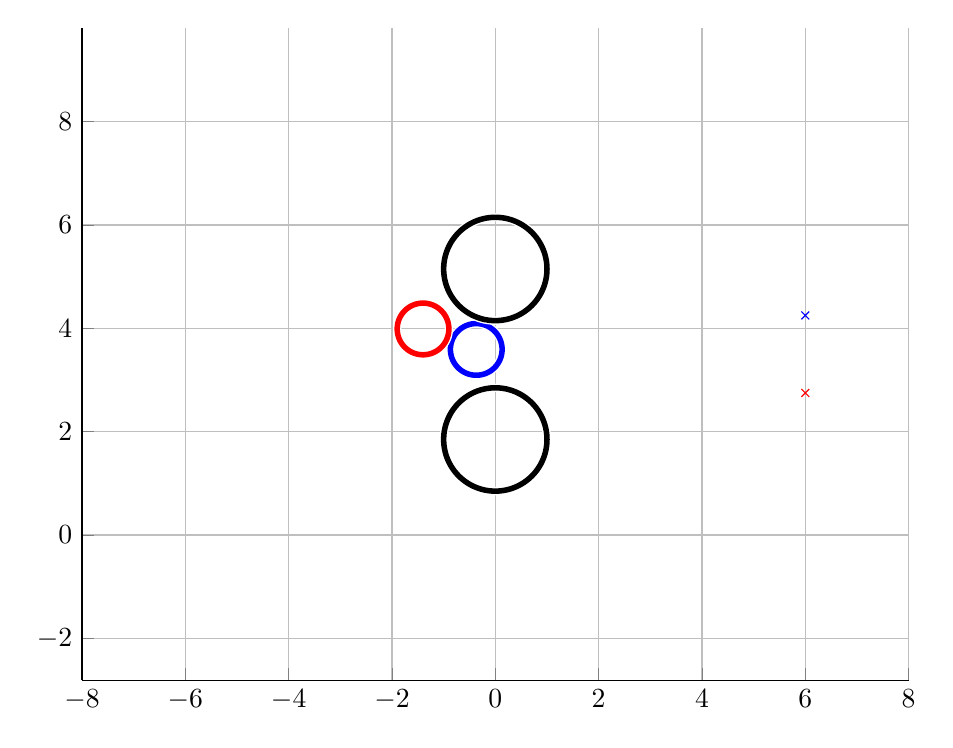
\begin{tikzpicture}

\begin{axis}[%
width=4.133in,
height=3.26in,
at={(0.693in,0.44in)},
scale only axis,
unbounded coords=jump,
xmin=-8,
xmax=8,
xmajorgrids,
ymin=-2.80967741935484,
ymax=9.80967741935484,
ymajorgrids,
axis background/.style={fill=white},
axis x line*=bottom,
axis y line*=left
]
\addplot [color=blue,only marks,mark=x,mark options={solid},forget plot]
  table[row sep=crcr]{%
6	4.25\\
};
\addplot [color=red,only marks,mark=x,mark options={solid},forget plot]
  table[row sep=crcr]{%
6	2.75\\
};
\addplot [color=white,solid,line width=3.0pt,forget plot]
  table[row sep=crcr]{%
0.130897460781974	3.59315597584639\\
0.130592874291521	3.61060572419764\\
0.129679485911886	3.62803421271845\\
0.12815840846611	3.64542020748022\\
0.126031495152759	3.66274252632642\\
0.123301337288078	3.67998006467986\\
0.119971261148876	3.69711182125527\\
0.116045323919972	3.71411692364622\\
0.111528308751133	3.73097465375489\\
0.10642571892955	3.74766447303386\\
0.100743771174928	3.76416604750922\\
0.0944893880653672	3.78045927255435\\
0.0876701896032739	3.79652429738429\\
0.080294483931557	3.81234154924093\\
0.072371257211437	3.82789175723934\\
0.0639101626741929	3.84315597584639\\
0.0549215088601865	3.85811560796299\\
0.0454162470594943	3.87275242758176\\
0.0354059579694472	3.88704860199263\\
0.0249028375853345	3.90098671350922\\
0.0139196823414625	3.91454978068966\\
0.00246987352067063	3.92772127902582\\
-0.0094326390487009	3.94048516107589\\
-0.0217733539885278	3.95282587601572\\
-0.0345372360385974	3.96472838858509\\
-0.0477087343747568	3.97617819740588\\
-0.0612718015551973	3.98716135264975\\
-0.0752099130717899	3.99766447303386\\
-0.0895060874826531	4.00767476212391\\
-0.104142907101424	4.0171800239246\\
-0.119102539218026	4.02616867773861\\
-0.134366757825081	4.03462977227585\\
-0.149916965823488	4.04255299899597\\
-0.165734217680126	4.04992870466769\\
-0.181799242510071	4.05674790312978\\
-0.198092467555192	4.06300228623935\\
-0.214594042030553	4.06868423399397\\
-0.231283861309527	4.07378682381555\\
-0.248141591418193	4.07830383898439\\
-0.265146693809147	4.08222977621329\\
-0.282278450384561	4.08555985235249\\
-0.299515988737994	4.08829001021718\\
-0.3168383075842	4.09041692353053\\
-0.334224302345964	4.0919380009763\\
-0.351652790866776	4.09285138935594\\
-0.369102539218026	4.09315597584639\\
-0.386552287569277	4.09285138935594\\
-0.403980776090089	4.0919380009763\\
-0.421366770851853	4.09041692353053\\
-0.438689089698059	4.08829001021718\\
-0.455926628051492	4.08555985235249\\
-0.473058384626906	4.08222977621329\\
-0.49006348701786	4.07830383898439\\
-0.506921217126526	4.07378682381555\\
-0.5236110364055	4.06868423399397\\
-0.540112610880861	4.06300228623935\\
-0.556405835925982	4.05674790312978\\
-0.572470860755927	4.04992870466769\\
-0.588288112612565	4.04255299899597\\
-0.603838320610972	4.03462977227585\\
-0.619102539218026	4.02616867773861\\
-0.634062171334629	4.0171800239246\\
-0.6486989909534	4.00767476212391\\
-0.662995165364263	3.99766447303386\\
-0.676933276880856	3.98716135264975\\
-0.690496344061296	3.97617819740588\\
-0.703667842397456	3.96472838858509\\
-0.716431724447525	3.95282587601572\\
-0.728772439387352	3.94048516107589\\
-0.740674951956724	3.92772127902582\\
-0.752124760777515	3.91454978068966\\
-0.763107916021387	3.90098671350922\\
-0.7736110364055	3.88704860199263\\
-0.783621325495547	3.87275242758176\\
-0.793126587296239	3.85811560796299\\
-0.802115241110246	3.84315597584639\\
-0.81057633564749	3.82789175723934\\
-0.81849956236761	3.81234154924093\\
-0.825875268039327	3.79652429738429\\
-0.83269446650142	3.78045927255435\\
-0.838948849610981	3.76416604750923\\
-0.844630797365603	3.74766447303386\\
-0.849733387187186	3.73097465375489\\
-0.854250402356025	3.71411692364622\\
-0.858176339584929	3.69711182125527\\
-0.861506415724131	3.67998006467986\\
-0.864236573588812	3.66274252632642\\
-0.866363486902163	3.64542020748022\\
-0.867884564347939	3.62803421271845\\
-0.868797952727574	3.61060572419764\\
-0.869102539218026	3.59315597584639\\
-0.868797952727574	3.57570622749514\\
-0.867884564347939	3.55827773897433\\
-0.866363486902163	3.54089174421256\\
-0.864236573588812	3.52356942536636\\
-0.861506415724131	3.50633188701293\\
-0.858176339584929	3.48920013043751\\
-0.854250402356025	3.47219502804656\\
-0.849733387187186	3.45533729793789\\
-0.844630797365603	3.43864747865892\\
-0.838948849610981	3.42214590418356\\
-0.83269446650142	3.40585267913843\\
-0.825875268039327	3.38978765430849\\
-0.81849956236761	3.37397040245185\\
-0.81057633564749	3.35842019445345\\
-0.802115241110246	3.34315597584639\\
-0.79312658729624	3.32819634372979\\
-0.783621325495547	3.31355952411102\\
-0.7736110364055	3.29926334970015\\
-0.763107916021388	3.28532523818356\\
-0.752124760777516	3.27176217100312\\
-0.740674951956724	3.25859067266696\\
-0.728772439387352	3.24582679061689\\
-0.716431724447525	3.23348607567707\\
-0.703667842397456	3.22158356310769\\
-0.690496344061296	3.2101337542869\\
-0.676933276880856	3.19915059904303\\
-0.662995165364263	3.18864747865892\\
-0.6486989909534	3.17863718956887\\
-0.634062171334629	3.16913192776818\\
-0.619102539218027	3.16014327395417\\
-0.603838320610972	3.15168217941693\\
-0.588288112612565	3.14375895269681\\
-0.572470860755927	3.13638324702509\\
-0.556405835925983	3.129564048563\\
-0.540112610880861	3.12330966545344\\
-0.5236110364055	3.11762771769881\\
-0.506921217126526	3.11252512787723\\
-0.49006348701786	3.10800811270839\\
-0.473058384626906	3.10408217547949\\
-0.455926628051492	3.10075209934029\\
-0.438689089698059	3.09802194147561\\
-0.421366770851853	3.09589502816225\\
-0.403980776090089	3.09437395071648\\
-0.386552287569277	3.09346056233684\\
-0.369102539218027	3.09315597584639\\
-0.351652790866776	3.09346056233684\\
-0.334224302345964	3.09437395071648\\
-0.3168383075842	3.09589502816225\\
-0.299515988737994	3.09802194147561\\
-0.282278450384562	3.10075209934029\\
-0.265146693809147	3.10408217547949\\
-0.248141591418193	3.10800811270839\\
-0.231283861309527	3.11252512787723\\
-0.214594042030553	3.11762771769881\\
-0.198092467555192	3.12330966545344\\
-0.181799242510071	3.129564048563\\
-0.165734217680126	3.13638324702509\\
-0.149916965823488	3.14375895269681\\
-0.134366757825081	3.15168217941693\\
-0.119102539218026	3.16014327395417\\
-0.104142907101424	3.16913192776818\\
-0.0895060874826534	3.17863718956887\\
-0.07520991307179	3.18864747865892\\
-0.0612718015551972	3.19915059904303\\
-0.0477087343747569	3.2101337542869\\
-0.0345372360385976	3.22158356310769\\
-0.0217733539885282	3.23348607567706\\
-0.00943263904870106	3.24582679061689\\
0.00246987352067063	3.25859067266696\\
0.0139196823414624	3.27176217100312\\
0.0249028375853343	3.28532523818356\\
0.0354059579694472	3.29926334970015\\
0.0454162470594942	3.31355952411102\\
0.0549215088601862	3.32819634372979\\
0.0639101626741927	3.34315597584639\\
0.072371257211437	3.35842019445345\\
0.0802944839315571	3.37397040245185\\
0.087670189603274	3.38978765430849\\
0.0944893880653672	3.40585267913843\\
0.100743771174928	3.42214590418356\\
0.10642571892955	3.43864747865892\\
0.111528308751133	3.45533729793789\\
0.116045323919972	3.47219502804656\\
0.119971261148876	3.48920013043751\\
0.123301337288077	3.50633188701293\\
0.126031495152759	3.52356942536636\\
0.12815840846611	3.54089174421256\\
0.129679485911886	3.55827773897433\\
0.130592874291521	3.57570622749514\\
0.130897460781974	3.59315597584639\\
nan	nan\\
};
\addplot [color=blue,solid,line width=2.0pt,forget plot]
  table[row sep=crcr]{%
0.130897460781974	3.59315597584639\\
0.130592874291521	3.61060572419764\\
0.129679485911886	3.62803421271845\\
0.12815840846611	3.64542020748022\\
0.126031495152759	3.66274252632642\\
0.123301337288078	3.67998006467986\\
0.119971261148876	3.69711182125527\\
0.116045323919972	3.71411692364622\\
0.111528308751133	3.73097465375489\\
0.10642571892955	3.74766447303386\\
0.100743771174928	3.76416604750922\\
0.0944893880653672	3.78045927255435\\
0.0876701896032739	3.79652429738429\\
0.080294483931557	3.81234154924093\\
0.072371257211437	3.82789175723934\\
0.0639101626741929	3.84315597584639\\
0.0549215088601865	3.85811560796299\\
0.0454162470594943	3.87275242758176\\
0.0354059579694472	3.88704860199263\\
0.0249028375853345	3.90098671350922\\
0.0139196823414625	3.91454978068966\\
0.00246987352067063	3.92772127902582\\
-0.0094326390487009	3.94048516107589\\
-0.0217733539885278	3.95282587601572\\
-0.0345372360385974	3.96472838858509\\
-0.0477087343747568	3.97617819740588\\
-0.0612718015551973	3.98716135264975\\
-0.0752099130717899	3.99766447303386\\
-0.0895060874826531	4.00767476212391\\
-0.104142907101424	4.0171800239246\\
-0.119102539218026	4.02616867773861\\
-0.134366757825081	4.03462977227585\\
-0.149916965823488	4.04255299899597\\
-0.165734217680126	4.04992870466769\\
-0.181799242510071	4.05674790312978\\
-0.198092467555192	4.06300228623935\\
-0.214594042030553	4.06868423399397\\
-0.231283861309527	4.07378682381555\\
-0.248141591418193	4.07830383898439\\
-0.265146693809147	4.08222977621329\\
-0.282278450384561	4.08555985235249\\
-0.299515988737994	4.08829001021718\\
-0.3168383075842	4.09041692353053\\
-0.334224302345964	4.0919380009763\\
-0.351652790866776	4.09285138935594\\
-0.369102539218026	4.09315597584639\\
-0.386552287569277	4.09285138935594\\
-0.403980776090089	4.0919380009763\\
-0.421366770851853	4.09041692353053\\
-0.438689089698059	4.08829001021718\\
-0.455926628051492	4.08555985235249\\
-0.473058384626906	4.08222977621329\\
-0.49006348701786	4.07830383898439\\
-0.506921217126526	4.07378682381555\\
-0.5236110364055	4.06868423399397\\
-0.540112610880861	4.06300228623935\\
-0.556405835925982	4.05674790312978\\
-0.572470860755927	4.04992870466769\\
-0.588288112612565	4.04255299899597\\
-0.603838320610972	4.03462977227585\\
-0.619102539218026	4.02616867773861\\
-0.634062171334629	4.0171800239246\\
-0.6486989909534	4.00767476212391\\
-0.662995165364263	3.99766447303386\\
-0.676933276880856	3.98716135264975\\
-0.690496344061296	3.97617819740588\\
-0.703667842397456	3.96472838858509\\
-0.716431724447525	3.95282587601572\\
-0.728772439387352	3.94048516107589\\
-0.740674951956724	3.92772127902582\\
-0.752124760777515	3.91454978068966\\
-0.763107916021387	3.90098671350922\\
-0.7736110364055	3.88704860199263\\
-0.783621325495547	3.87275242758176\\
-0.793126587296239	3.85811560796299\\
-0.802115241110246	3.84315597584639\\
-0.81057633564749	3.82789175723934\\
-0.81849956236761	3.81234154924093\\
-0.825875268039327	3.79652429738429\\
-0.83269446650142	3.78045927255435\\
-0.838948849610981	3.76416604750923\\
-0.844630797365603	3.74766447303386\\
-0.849733387187186	3.73097465375489\\
-0.854250402356025	3.71411692364622\\
-0.858176339584929	3.69711182125527\\
-0.861506415724131	3.67998006467986\\
-0.864236573588812	3.66274252632642\\
-0.866363486902163	3.64542020748022\\
-0.867884564347939	3.62803421271845\\
-0.868797952727574	3.61060572419764\\
-0.869102539218026	3.59315597584639\\
-0.868797952727574	3.57570622749514\\
-0.867884564347939	3.55827773897433\\
-0.866363486902163	3.54089174421256\\
-0.864236573588812	3.52356942536636\\
-0.861506415724131	3.50633188701293\\
-0.858176339584929	3.48920013043751\\
-0.854250402356025	3.47219502804656\\
-0.849733387187186	3.45533729793789\\
-0.844630797365603	3.43864747865892\\
-0.838948849610981	3.42214590418356\\
-0.83269446650142	3.40585267913843\\
-0.825875268039327	3.38978765430849\\
-0.81849956236761	3.37397040245185\\
-0.81057633564749	3.35842019445345\\
-0.802115241110246	3.34315597584639\\
-0.79312658729624	3.32819634372979\\
-0.783621325495547	3.31355952411102\\
-0.7736110364055	3.29926334970015\\
-0.763107916021388	3.28532523818356\\
-0.752124760777516	3.27176217100312\\
-0.740674951956724	3.25859067266696\\
-0.728772439387352	3.24582679061689\\
-0.716431724447525	3.23348607567707\\
-0.703667842397456	3.22158356310769\\
-0.690496344061296	3.2101337542869\\
-0.676933276880856	3.19915059904303\\
-0.662995165364263	3.18864747865892\\
-0.6486989909534	3.17863718956887\\
-0.634062171334629	3.16913192776818\\
-0.619102539218027	3.16014327395417\\
-0.603838320610972	3.15168217941693\\
-0.588288112612565	3.14375895269681\\
-0.572470860755927	3.13638324702509\\
-0.556405835925983	3.129564048563\\
-0.540112610880861	3.12330966545344\\
-0.5236110364055	3.11762771769881\\
-0.506921217126526	3.11252512787723\\
-0.49006348701786	3.10800811270839\\
-0.473058384626906	3.10408217547949\\
-0.455926628051492	3.10075209934029\\
-0.438689089698059	3.09802194147561\\
-0.421366770851853	3.09589502816225\\
-0.403980776090089	3.09437395071648\\
-0.386552287569277	3.09346056233684\\
-0.369102539218027	3.09315597584639\\
-0.351652790866776	3.09346056233684\\
-0.334224302345964	3.09437395071648\\
-0.3168383075842	3.09589502816225\\
-0.299515988737994	3.09802194147561\\
-0.282278450384562	3.10075209934029\\
-0.265146693809147	3.10408217547949\\
-0.248141591418193	3.10800811270839\\
-0.231283861309527	3.11252512787723\\
-0.214594042030553	3.11762771769881\\
-0.198092467555192	3.12330966545344\\
-0.181799242510071	3.129564048563\\
-0.165734217680126	3.13638324702509\\
-0.149916965823488	3.14375895269681\\
-0.134366757825081	3.15168217941693\\
-0.119102539218026	3.16014327395417\\
-0.104142907101424	3.16913192776818\\
-0.0895060874826534	3.17863718956887\\
-0.07520991307179	3.18864747865892\\
-0.0612718015551972	3.19915059904303\\
-0.0477087343747569	3.2101337542869\\
-0.0345372360385976	3.22158356310769\\
-0.0217733539885282	3.23348607567706\\
-0.00943263904870106	3.24582679061689\\
0.00246987352067063	3.25859067266696\\
0.0139196823414624	3.27176217100312\\
0.0249028375853343	3.28532523818356\\
0.0354059579694472	3.29926334970015\\
0.0454162470594942	3.31355952411102\\
0.0549215088601862	3.32819634372979\\
0.0639101626741927	3.34315597584639\\
0.072371257211437	3.35842019445345\\
0.0802944839315571	3.37397040245185\\
0.087670189603274	3.38978765430849\\
0.0944893880653672	3.40585267913843\\
0.100743771174928	3.42214590418356\\
0.10642571892955	3.43864747865892\\
0.111528308751133	3.45533729793789\\
0.116045323919972	3.47219502804656\\
0.119971261148876	3.48920013043751\\
0.123301337288077	3.50633188701293\\
0.126031495152759	3.52356942536636\\
0.12815840846611	3.54089174421256\\
0.129679485911886	3.55827773897433\\
0.130592874291521	3.57570622749514\\
0.130897460781974	3.59315597584639\\
nan	nan\\
};
\addplot [color=white,solid,line width=3.0pt,forget plot]
  table[row sep=crcr]{%
-0.899246247926416	3.98908209419202\\
-0.899550834416868	4.00653184254327\\
-0.900464222796504	4.02396033106408\\
-0.901985300242279	4.04134632582585\\
-0.904112213555631	4.05866864467205\\
-0.906842371420312	4.07590618302548\\
-0.910172447559513	4.0930379396009\\
-0.914098384788418	4.11004304199185\\
-0.918615399957257	4.12690077210052\\
-0.923717989778839	4.14359059137949\\
-0.929399937533462	4.16009216585485\\
-0.935654320643022	4.17638539089997\\
-0.942473519105116	4.19245041572992\\
-0.949849224776833	4.20826766758656\\
-0.957772451496953	4.22381787558496\\
-0.966233546034197	4.23908209419202\\
-0.975222199848203	4.25404172630862\\
-0.984727461648895	4.26867854592739\\
-0.994737750738942	4.28297472033826\\
-1.00524087112306	4.29691283185485\\
-1.01622402636693	4.31047589903529\\
-1.02767383518772	4.32364739737145\\
-1.03957634775709	4.33641127942152\\
-1.05191706269692	4.34875199436134\\
-1.06468094474699	4.36065450693072\\
-1.07785244308315	4.37210431575151\\
-1.09141551026359	4.38308747099538\\
-1.10535362178018	4.39359059137949\\
-1.11964979619104	4.40360088046954\\
-1.13428661580981	4.41310614227023\\
-1.14924624792642	4.42209479608424\\
-1.16451046653347	4.43055589062148\\
-1.18006067453188	4.4384791173416\\
-1.19587792638852	4.44585482301332\\
-1.21194295121846	4.45267402147541\\
-1.22823617626358	4.45892840458497\\
-1.24473775073894	4.4646103523396\\
-1.26142757001792	4.46971294216118\\
-1.27828530012658	4.47422995733002\\
-1.29529040251754	4.47815589455892\\
-1.31242215909295	4.48148597069812\\
-1.32965969744638	4.4842161285628\\
-1.34698201629259	4.48634304187615\\
-1.36436801105435	4.48786411932193\\
-1.38179649957517	4.48877750770157\\
-1.39924624792642	4.48908209419202\\
-1.41669599627767	4.48877750770157\\
-1.43412448479848	4.48786411932193\\
-1.45151047956024	4.48634304187615\\
-1.46883279840645	4.4842161285628\\
-1.48607033675988	4.48148597069812\\
-1.5032020933353	4.47815589455892\\
-1.52020719572625	4.47422995733002\\
-1.53706492583492	4.46971294216118\\
-1.55375474511389	4.4646103523396\\
-1.57025631958925	4.45892840458497\\
-1.58654954463437	4.45267402147541\\
-1.60261456946432	4.44585482301332\\
-1.61843182132095	4.4384791173416\\
-1.63398202931936	4.43055589062148\\
-1.64924624792642	4.42209479608424\\
-1.66420588004302	4.41310614227023\\
-1.67884269966179	4.40360088046954\\
-1.69313887407265	4.39359059137949\\
-1.70707698558925	4.38308747099538\\
-1.72064005276969	4.37210431575151\\
-1.73381155110585	4.36065450693072\\
-1.74657543315591	4.34875199436134\\
-1.75891614809574	4.33641127942152\\
-1.77081866066511	4.32364739737145\\
-1.78226846948591	4.31047589903529\\
-1.79325162472978	4.29691283185485\\
-1.80375474511389	4.28297472033826\\
-1.81376503420394	4.26867854592739\\
-1.82327029600463	4.25404172630862\\
-1.83225894981864	4.23908209419202\\
-1.84072004435588	4.22381787558496\\
-1.848643271076	4.20826766758656\\
-1.85601897674772	4.19245041572992\\
-1.86283817520981	4.17638539089997\\
-1.86909255831937	4.16009216585485\\
-1.87477450607399	4.14359059137949\\
-1.87987709589558	4.12690077210052\\
-1.88439411106441	4.11004304199185\\
-1.88832004829332	4.0930379396009\\
-1.89165012443252	4.07590618302548\\
-1.8943802822972	4.05866864467205\\
-1.89650719561055	4.04134632582585\\
-1.89802827305633	4.02396033106408\\
-1.89894166143596	4.00653184254327\\
-1.89924624792642	3.98908209419202\\
-1.89894166143596	3.97163234584077\\
-1.89802827305633	3.95420385731996\\
-1.89650719561055	3.93681786255819\\
-1.8943802822972	3.91949554371199\\
-1.89165012443252	3.90225800535855\\
-1.88832004829332	3.88512624878314\\
-1.88439411106441	3.86812114639218\\
-1.87987709589558	3.85126341628352\\
-1.87477450607399	3.83457359700454\\
-1.86909255831937	3.81807202252918\\
-1.86283817520981	3.80177879748406\\
-1.85601897674772	3.78571377265412\\
-1.848643271076	3.76989652079748\\
-1.84072004435588	3.75434631279907\\
-1.83225894981864	3.73908209419202\\
-1.82327029600463	3.72412246207542\\
-1.81376503420394	3.70948564245665\\
-1.80375474511389	3.69518946804578\\
-1.79325162472978	3.68125135652919\\
-1.78226846948591	3.66768828934875\\
-1.77081866066511	3.65451679101259\\
-1.75891614809574	3.64175290896252\\
-1.74657543315591	3.62941219402269\\
-1.73381155110585	3.61750968145332\\
-1.72064005276969	3.60605987263253\\
-1.70707698558925	3.59507671738866\\
-1.69313887407265	3.58457359700454\\
-1.67884269966179	3.5745633079145\\
-1.66420588004302	3.56505804611381\\
-1.64924624792642	3.5560693922998\\
-1.63398202931936	3.54760829776255\\
-1.61843182132095	3.53968507104244\\
-1.60261456946432	3.53230936537072\\
-1.58654954463437	3.52549016690862\\
-1.57025631958925	3.51923578379906\\
-1.55375474511389	3.51355383604444\\
-1.53706492583492	3.50845124622286\\
-1.52020719572625	3.50393423105402\\
-1.5032020933353	3.50000829382512\\
-1.48607033675988	3.49667821768591\\
-1.46883279840645	3.49394805982123\\
-1.45151047956024	3.49182114650788\\
-1.43412448479848	3.49030006906211\\
-1.41669599627767	3.48938668068247\\
-1.39924624792642	3.48908209419202\\
-1.38179649957517	3.48938668068247\\
-1.36436801105435	3.49030006906211\\
-1.34698201629259	3.49182114650788\\
-1.32965969744638	3.49394805982123\\
-1.31242215909295	3.49667821768591\\
-1.29529040251754	3.50000829382512\\
-1.27828530012658	3.50393423105402\\
-1.26142757001792	3.50845124622286\\
-1.24473775073894	3.51355383604444\\
-1.22823617626358	3.51923578379906\\
-1.21194295121846	3.52549016690862\\
-1.19587792638852	3.53230936537072\\
-1.18006067453188	3.53968507104244\\
-1.16451046653347	3.54760829776255\\
-1.14924624792642	3.5560693922998\\
-1.13428661580981	3.56505804611381\\
-1.11964979619104	3.5745633079145\\
-1.10535362178018	3.58457359700454\\
-1.09141551026359	3.59507671738866\\
-1.07785244308315	3.60605987263253\\
-1.06468094474699	3.61750968145332\\
-1.05191706269692	3.62941219402269\\
-1.03957634775709	3.64175290896252\\
-1.02767383518772	3.65451679101259\\
-1.01622402636693	3.66768828934875\\
-1.00524087112306	3.68125135652919\\
-0.994737750738942	3.69518946804578\\
-0.984727461648895	3.70948564245664\\
-0.975222199848203	3.72412246207542\\
-0.966233546034197	3.73908209419202\\
-0.957772451496953	3.75434631279907\\
-0.949849224776832	3.76989652079748\\
-0.942473519105116	3.78571377265412\\
-0.935654320643022	3.80177879748406\\
-0.929399937533462	3.81807202252918\\
-0.923717989778839	3.83457359700454\\
-0.918615399957257	3.85126341628352\\
-0.914098384788418	3.86812114639218\\
-0.910172447559513	3.88512624878314\\
-0.906842371420312	3.90225800535855\\
-0.904112213555631	3.91949554371199\\
-0.901985300242279	3.93681786255819\\
-0.900464222796504	3.95420385731996\\
-0.899550834416868	3.97163234584077\\
-0.899246247926416	3.98908209419202\\
nan	nan\\
};
\addplot [color=red,solid,line width=2.0pt,forget plot]
  table[row sep=crcr]{%
-0.899246247926416	3.98908209419202\\
-0.899550834416868	4.00653184254327\\
-0.900464222796504	4.02396033106408\\
-0.901985300242279	4.04134632582585\\
-0.904112213555631	4.05866864467205\\
-0.906842371420312	4.07590618302548\\
-0.910172447559513	4.0930379396009\\
-0.914098384788418	4.11004304199185\\
-0.918615399957257	4.12690077210052\\
-0.923717989778839	4.14359059137949\\
-0.929399937533462	4.16009216585485\\
-0.935654320643022	4.17638539089997\\
-0.942473519105116	4.19245041572992\\
-0.949849224776833	4.20826766758656\\
-0.957772451496953	4.22381787558496\\
-0.966233546034197	4.23908209419202\\
-0.975222199848203	4.25404172630862\\
-0.984727461648895	4.26867854592739\\
-0.994737750738942	4.28297472033826\\
-1.00524087112306	4.29691283185485\\
-1.01622402636693	4.31047589903529\\
-1.02767383518772	4.32364739737145\\
-1.03957634775709	4.33641127942152\\
-1.05191706269692	4.34875199436134\\
-1.06468094474699	4.36065450693072\\
-1.07785244308315	4.37210431575151\\
-1.09141551026359	4.38308747099538\\
-1.10535362178018	4.39359059137949\\
-1.11964979619104	4.40360088046954\\
-1.13428661580981	4.41310614227023\\
-1.14924624792642	4.42209479608424\\
-1.16451046653347	4.43055589062148\\
-1.18006067453188	4.4384791173416\\
-1.19587792638852	4.44585482301332\\
-1.21194295121846	4.45267402147541\\
-1.22823617626358	4.45892840458497\\
-1.24473775073894	4.4646103523396\\
-1.26142757001792	4.46971294216118\\
-1.27828530012658	4.47422995733002\\
-1.29529040251754	4.47815589455892\\
-1.31242215909295	4.48148597069812\\
-1.32965969744638	4.4842161285628\\
-1.34698201629259	4.48634304187615\\
-1.36436801105435	4.48786411932193\\
-1.38179649957517	4.48877750770157\\
-1.39924624792642	4.48908209419202\\
-1.41669599627767	4.48877750770157\\
-1.43412448479848	4.48786411932193\\
-1.45151047956024	4.48634304187615\\
-1.46883279840645	4.4842161285628\\
-1.48607033675988	4.48148597069812\\
-1.5032020933353	4.47815589455892\\
-1.52020719572625	4.47422995733002\\
-1.53706492583492	4.46971294216118\\
-1.55375474511389	4.4646103523396\\
-1.57025631958925	4.45892840458497\\
-1.58654954463437	4.45267402147541\\
-1.60261456946432	4.44585482301332\\
-1.61843182132095	4.4384791173416\\
-1.63398202931936	4.43055589062148\\
-1.64924624792642	4.42209479608424\\
-1.66420588004302	4.41310614227023\\
-1.67884269966179	4.40360088046954\\
-1.69313887407265	4.39359059137949\\
-1.70707698558925	4.38308747099538\\
-1.72064005276969	4.37210431575151\\
-1.73381155110585	4.36065450693072\\
-1.74657543315591	4.34875199436134\\
-1.75891614809574	4.33641127942152\\
-1.77081866066511	4.32364739737145\\
-1.78226846948591	4.31047589903529\\
-1.79325162472978	4.29691283185485\\
-1.80375474511389	4.28297472033826\\
-1.81376503420394	4.26867854592739\\
-1.82327029600463	4.25404172630862\\
-1.83225894981864	4.23908209419202\\
-1.84072004435588	4.22381787558496\\
-1.848643271076	4.20826766758656\\
-1.85601897674772	4.19245041572992\\
-1.86283817520981	4.17638539089997\\
-1.86909255831937	4.16009216585485\\
-1.87477450607399	4.14359059137949\\
-1.87987709589558	4.12690077210052\\
-1.88439411106441	4.11004304199185\\
-1.88832004829332	4.0930379396009\\
-1.89165012443252	4.07590618302548\\
-1.8943802822972	4.05866864467205\\
-1.89650719561055	4.04134632582585\\
-1.89802827305633	4.02396033106408\\
-1.89894166143596	4.00653184254327\\
-1.89924624792642	3.98908209419202\\
-1.89894166143596	3.97163234584077\\
-1.89802827305633	3.95420385731996\\
-1.89650719561055	3.93681786255819\\
-1.8943802822972	3.91949554371199\\
-1.89165012443252	3.90225800535855\\
-1.88832004829332	3.88512624878314\\
-1.88439411106441	3.86812114639218\\
-1.87987709589558	3.85126341628352\\
-1.87477450607399	3.83457359700454\\
-1.86909255831937	3.81807202252918\\
-1.86283817520981	3.80177879748406\\
-1.85601897674772	3.78571377265412\\
-1.848643271076	3.76989652079748\\
-1.84072004435588	3.75434631279907\\
-1.83225894981864	3.73908209419202\\
-1.82327029600463	3.72412246207542\\
-1.81376503420394	3.70948564245665\\
-1.80375474511389	3.69518946804578\\
-1.79325162472978	3.68125135652919\\
-1.78226846948591	3.66768828934875\\
-1.77081866066511	3.65451679101259\\
-1.75891614809574	3.64175290896252\\
-1.74657543315591	3.62941219402269\\
-1.73381155110585	3.61750968145332\\
-1.72064005276969	3.60605987263253\\
-1.70707698558925	3.59507671738866\\
-1.69313887407265	3.58457359700454\\
-1.67884269966179	3.5745633079145\\
-1.66420588004302	3.56505804611381\\
-1.64924624792642	3.5560693922998\\
-1.63398202931936	3.54760829776255\\
-1.61843182132095	3.53968507104244\\
-1.60261456946432	3.53230936537072\\
-1.58654954463437	3.52549016690862\\
-1.57025631958925	3.51923578379906\\
-1.55375474511389	3.51355383604444\\
-1.53706492583492	3.50845124622286\\
-1.52020719572625	3.50393423105402\\
-1.5032020933353	3.50000829382512\\
-1.48607033675988	3.49667821768591\\
-1.46883279840645	3.49394805982123\\
-1.45151047956024	3.49182114650788\\
-1.43412448479848	3.49030006906211\\
-1.41669599627767	3.48938668068247\\
-1.39924624792642	3.48908209419202\\
-1.38179649957517	3.48938668068247\\
-1.36436801105435	3.49030006906211\\
-1.34698201629259	3.49182114650788\\
-1.32965969744638	3.49394805982123\\
-1.31242215909295	3.49667821768591\\
-1.29529040251754	3.50000829382512\\
-1.27828530012658	3.50393423105402\\
-1.26142757001792	3.50845124622286\\
-1.24473775073894	3.51355383604444\\
-1.22823617626358	3.51923578379906\\
-1.21194295121846	3.52549016690862\\
-1.19587792638852	3.53230936537072\\
-1.18006067453188	3.53968507104244\\
-1.16451046653347	3.54760829776255\\
-1.14924624792642	3.5560693922998\\
-1.13428661580981	3.56505804611381\\
-1.11964979619104	3.5745633079145\\
-1.10535362178018	3.58457359700454\\
-1.09141551026359	3.59507671738866\\
-1.07785244308315	3.60605987263253\\
-1.06468094474699	3.61750968145332\\
-1.05191706269692	3.62941219402269\\
-1.03957634775709	3.64175290896252\\
-1.02767383518772	3.65451679101259\\
-1.01622402636693	3.66768828934875\\
-1.00524087112306	3.68125135652919\\
-0.994737750738942	3.69518946804578\\
-0.984727461648895	3.70948564245664\\
-0.975222199848203	3.72412246207542\\
-0.966233546034197	3.73908209419202\\
-0.957772451496953	3.75434631279907\\
-0.949849224776832	3.76989652079748\\
-0.942473519105116	3.78571377265412\\
-0.935654320643022	3.80177879748406\\
-0.929399937533462	3.81807202252918\\
-0.923717989778839	3.83457359700454\\
-0.918615399957257	3.85126341628352\\
-0.914098384788418	3.86812114639218\\
-0.910172447559513	3.88512624878314\\
-0.906842371420312	3.90225800535855\\
-0.904112213555631	3.91949554371199\\
-0.901985300242279	3.93681786255819\\
-0.900464222796504	3.95420385731996\\
-0.899550834416868	3.97163234584077\\
-0.899246247926416	3.98908209419202\\
nan	nan\\
};
\addplot [color=white,solid,line width=3.0pt,forget plot]
  table[row sep=crcr]{%
1	1.85\\
0.999390827019096	1.8848994967025\\
0.997564050259824	1.91975647374413\\
0.994521895368273	1.95452846326765\\
0.99026806874157	1.98917310096007\\
0.984807753012208	2.02364817766693\\
0.978147600733806	2.05791169081776\\
0.970295726275996	2.09192189559967\\
0.961261695938319	2.125637355817\\
0.951056516295154	2.15901699437495\\
0.939692620785908	2.19202014332567\\
0.927183854566787	2.22460659341591\\
0.913545457642601	2.2567366430758\\
0.898794046299167	2.28837114678908\\
0.882947592858927	2.31947156278589\\
0.866025403784439	2.35\\
0.848048096156426	2.37991926423321\\
0.829037572555042	2.40919290347075\\
0.809016994374947	2.43778525229247\\
0.788010753606722	2.46566147532566\\
0.766044443118978	2.49278760968654\\
0.743144825477394	2.51913060635886\\
0.719339800338651	2.544658370459\\
0.694658370458997	2.56933980033865\\
0.669130606358858	2.59314482547739\\
0.642787609686539	2.61604444311898\\
0.615661475325658	2.63801075360672\\
0.587785252292473	2.65901699437495\\
0.559192903470747	2.67903757255504\\
0.529919264233205	2.69804809615643\\
0.5	2.71602540378444\\
0.469471562785891	2.73294759285893\\
0.438371146789077	2.74879404629917\\
0.4067366430758	2.7635454576426\\
0.374606593415912	2.77718385456679\\
0.342020143325669	2.78969262078591\\
0.309016994374947	2.80105651629515\\
0.275637355816999	2.81126169593832\\
0.241921895599668	2.820295726276\\
0.207911690817759	2.82814760073381\\
0.17364817766693	2.83480775301221\\
0.139173100960066	2.84026806874157\\
0.104528463267653	2.84452189536827\\
0.0697564737441255	2.84756405025982\\
0.0348994967025011	2.8493908270191\\
6.12323399573677e-17	2.85\\
-0.0348994967025007	2.8493908270191\\
-0.0697564737441253	2.84756405025982\\
-0.104528463267653	2.84452189536827\\
-0.139173100960065	2.84026806874157\\
-0.17364817766693	2.83480775301221\\
-0.207911690817759	2.82814760073381\\
-0.241921895599668	2.820295726276\\
-0.275637355816999	2.81126169593832\\
-0.309016994374947	2.80105651629515\\
-0.342020143325669	2.78969262078591\\
-0.374606593415912	2.77718385456679\\
-0.4067366430758	2.7635454576426\\
-0.438371146789078	2.74879404629917\\
-0.469471562785891	2.73294759285893\\
-0.5	2.71602540378444\\
-0.529919264233205	2.69804809615643\\
-0.559192903470747	2.67903757255504\\
-0.587785252292473	2.65901699437495\\
-0.615661475325658	2.63801075360672\\
-0.642787609686539	2.61604444311898\\
-0.669130606358858	2.59314482547739\\
-0.694658370458997	2.56933980033865\\
-0.719339800338651	2.544658370459\\
-0.743144825477394	2.51913060635886\\
-0.766044443118978	2.49278760968654\\
-0.788010753606722	2.46566147532566\\
-0.809016994374947	2.43778525229247\\
-0.829037572555042	2.40919290347075\\
-0.848048096156426	2.37991926423321\\
-0.866025403784439	2.35\\
-0.882947592858927	2.31947156278589\\
-0.898794046299167	2.28837114678908\\
-0.913545457642601	2.2567366430758\\
-0.927183854566787	2.22460659341591\\
-0.939692620785908	2.19202014332567\\
-0.951056516295154	2.15901699437495\\
-0.961261695938319	2.125637355817\\
-0.970295726275996	2.09192189559967\\
-0.978147600733806	2.05791169081776\\
-0.984807753012208	2.02364817766693\\
-0.99026806874157	1.98917310096007\\
-0.994521895368273	1.95452846326765\\
-0.997564050259824	1.91975647374413\\
-0.999390827019096	1.8848994967025\\
-1	1.85\\
-0.999390827019096	1.8151005032975\\
-0.997564050259824	1.78024352625588\\
-0.994521895368273	1.74547153673235\\
-0.99026806874157	1.71082689903993\\
-0.984807753012208	1.67635182233307\\
-0.978147600733806	1.64208830918224\\
-0.970295726275997	1.60807810440033\\
-0.961261695938319	1.574362644183\\
-0.951056516295154	1.54098300562505\\
-0.939692620785908	1.50797985667433\\
-0.927183854566787	1.47539340658409\\
-0.913545457642601	1.4432633569242\\
-0.898794046299167	1.41162885321092\\
-0.882947592858927	1.38052843721411\\
-0.866025403784439	1.35\\
-0.848048096156426	1.3200807357668\\
-0.829037572555042	1.29080709652925\\
-0.809016994374947	1.26221474770753\\
-0.788010753606722	1.23433852467434\\
-0.766044443118978	1.20721239031346\\
-0.743144825477394	1.18086939364114\\
-0.719339800338651	1.155341629541\\
-0.694658370458997	1.13066019966135\\
-0.669130606358858	1.10685517452261\\
-0.642787609686539	1.08395555688102\\
-0.615661475325658	1.06198924639328\\
-0.587785252292473	1.04098300562505\\
-0.559192903470747	1.02096242744496\\
-0.529919264233205	1.00195190384357\\
-0.5	0.983974596215562\\
-0.469471562785891	0.967052407141073\\
-0.438371146789078	0.951205953700833\\
-0.4067366430758	0.936454542357399\\
-0.374606593415912	0.922816145433213\\
-0.342020143325669	0.910307379214092\\
-0.309016994374948	0.898943483704847\\
-0.275637355816999	0.888738304061681\\
-0.241921895599668	0.879704273724004\\
-0.20791169081776	0.871852399266195\\
-0.17364817766693	0.865192246987792\\
-0.139173100960065	0.85973193125843\\
-0.104528463267653	0.855478104631727\\
-0.0697564737441256	0.852435949740176\\
-0.0348994967025016	0.850609172980904\\
-1.83697019872103e-16	0.85\\
0.0348994967025013	0.850609172980904\\
0.0697564737441252	0.852435949740176\\
0.104528463267653	0.855478104631727\\
0.139173100960065	0.85973193125843\\
0.17364817766693	0.865192246987792\\
0.207911690817759	0.871852399266194\\
0.241921895599667	0.879704273724004\\
0.275637355816999	0.888738304061681\\
0.309016994374947	0.898943483704846\\
0.342020143325668	0.910307379214092\\
0.374606593415912	0.922816145433213\\
0.406736643075801	0.936454542357399\\
0.438371146789077	0.951205953700833\\
0.46947156278589	0.967052407141073\\
0.5	0.983974596215561\\
0.529919264233205	1.00195190384357\\
0.559192903470746	1.02096242744496\\
0.587785252292473	1.04098300562505\\
0.615661475325659	1.06198924639328\\
0.642787609686539	1.08395555688102\\
0.669130606358858	1.10685517452261\\
0.694658370458997	1.13066019966135\\
0.719339800338651	1.155341629541\\
0.743144825477394	1.18086939364114\\
0.766044443118978	1.20721239031346\\
0.788010753606722	1.23433852467434\\
0.809016994374947	1.26221474770753\\
0.829037572555041	1.29080709652925\\
0.848048096156425	1.32008073576679\\
0.866025403784438	1.35\\
0.882947592858927	1.38052843721411\\
0.898794046299167	1.41162885321092\\
0.913545457642601	1.4432633569242\\
0.927183854566787	1.47539340658409\\
0.939692620785908	1.50797985667433\\
0.951056516295154	1.54098300562505\\
0.961261695938319	1.574362644183\\
0.970295726275996	1.60807810440033\\
0.978147600733806	1.64208830918224\\
0.984807753012208	1.67635182233307\\
0.99026806874157	1.71082689903993\\
0.994521895368273	1.74547153673235\\
0.997564050259824	1.78024352625588\\
0.999390827019096	1.8151005032975\\
1	1.85\\
nan	nan\\
};
\addplot [color=black,solid,line width=2.0pt,forget plot]
  table[row sep=crcr]{%
1	1.85\\
0.999390827019096	1.8848994967025\\
0.997564050259824	1.91975647374413\\
0.994521895368273	1.95452846326765\\
0.99026806874157	1.98917310096007\\
0.984807753012208	2.02364817766693\\
0.978147600733806	2.05791169081776\\
0.970295726275996	2.09192189559967\\
0.961261695938319	2.125637355817\\
0.951056516295154	2.15901699437495\\
0.939692620785908	2.19202014332567\\
0.927183854566787	2.22460659341591\\
0.913545457642601	2.2567366430758\\
0.898794046299167	2.28837114678908\\
0.882947592858927	2.31947156278589\\
0.866025403784439	2.35\\
0.848048096156426	2.37991926423321\\
0.829037572555042	2.40919290347075\\
0.809016994374947	2.43778525229247\\
0.788010753606722	2.46566147532566\\
0.766044443118978	2.49278760968654\\
0.743144825477394	2.51913060635886\\
0.719339800338651	2.544658370459\\
0.694658370458997	2.56933980033865\\
0.669130606358858	2.59314482547739\\
0.642787609686539	2.61604444311898\\
0.615661475325658	2.63801075360672\\
0.587785252292473	2.65901699437495\\
0.559192903470747	2.67903757255504\\
0.529919264233205	2.69804809615643\\
0.5	2.71602540378444\\
0.469471562785891	2.73294759285893\\
0.438371146789077	2.74879404629917\\
0.4067366430758	2.7635454576426\\
0.374606593415912	2.77718385456679\\
0.342020143325669	2.78969262078591\\
0.309016994374947	2.80105651629515\\
0.275637355816999	2.81126169593832\\
0.241921895599668	2.820295726276\\
0.207911690817759	2.82814760073381\\
0.17364817766693	2.83480775301221\\
0.139173100960066	2.84026806874157\\
0.104528463267653	2.84452189536827\\
0.0697564737441255	2.84756405025982\\
0.0348994967025011	2.8493908270191\\
6.12323399573677e-17	2.85\\
-0.0348994967025007	2.8493908270191\\
-0.0697564737441253	2.84756405025982\\
-0.104528463267653	2.84452189536827\\
-0.139173100960065	2.84026806874157\\
-0.17364817766693	2.83480775301221\\
-0.207911690817759	2.82814760073381\\
-0.241921895599668	2.820295726276\\
-0.275637355816999	2.81126169593832\\
-0.309016994374947	2.80105651629515\\
-0.342020143325669	2.78969262078591\\
-0.374606593415912	2.77718385456679\\
-0.4067366430758	2.7635454576426\\
-0.438371146789078	2.74879404629917\\
-0.469471562785891	2.73294759285893\\
-0.5	2.71602540378444\\
-0.529919264233205	2.69804809615643\\
-0.559192903470747	2.67903757255504\\
-0.587785252292473	2.65901699437495\\
-0.615661475325658	2.63801075360672\\
-0.642787609686539	2.61604444311898\\
-0.669130606358858	2.59314482547739\\
-0.694658370458997	2.56933980033865\\
-0.719339800338651	2.544658370459\\
-0.743144825477394	2.51913060635886\\
-0.766044443118978	2.49278760968654\\
-0.788010753606722	2.46566147532566\\
-0.809016994374947	2.43778525229247\\
-0.829037572555042	2.40919290347075\\
-0.848048096156426	2.37991926423321\\
-0.866025403784439	2.35\\
-0.882947592858927	2.31947156278589\\
-0.898794046299167	2.28837114678908\\
-0.913545457642601	2.2567366430758\\
-0.927183854566787	2.22460659341591\\
-0.939692620785908	2.19202014332567\\
-0.951056516295154	2.15901699437495\\
-0.961261695938319	2.125637355817\\
-0.970295726275996	2.09192189559967\\
-0.978147600733806	2.05791169081776\\
-0.984807753012208	2.02364817766693\\
-0.99026806874157	1.98917310096007\\
-0.994521895368273	1.95452846326765\\
-0.997564050259824	1.91975647374413\\
-0.999390827019096	1.8848994967025\\
-1	1.85\\
-0.999390827019096	1.8151005032975\\
-0.997564050259824	1.78024352625588\\
-0.994521895368273	1.74547153673235\\
-0.99026806874157	1.71082689903993\\
-0.984807753012208	1.67635182233307\\
-0.978147600733806	1.64208830918224\\
-0.970295726275997	1.60807810440033\\
-0.961261695938319	1.574362644183\\
-0.951056516295154	1.54098300562505\\
-0.939692620785908	1.50797985667433\\
-0.927183854566787	1.47539340658409\\
-0.913545457642601	1.4432633569242\\
-0.898794046299167	1.41162885321092\\
-0.882947592858927	1.38052843721411\\
-0.866025403784439	1.35\\
-0.848048096156426	1.3200807357668\\
-0.829037572555042	1.29080709652925\\
-0.809016994374947	1.26221474770753\\
-0.788010753606722	1.23433852467434\\
-0.766044443118978	1.20721239031346\\
-0.743144825477394	1.18086939364114\\
-0.719339800338651	1.155341629541\\
-0.694658370458997	1.13066019966135\\
-0.669130606358858	1.10685517452261\\
-0.642787609686539	1.08395555688102\\
-0.615661475325658	1.06198924639328\\
-0.587785252292473	1.04098300562505\\
-0.559192903470747	1.02096242744496\\
-0.529919264233205	1.00195190384357\\
-0.5	0.983974596215562\\
-0.469471562785891	0.967052407141073\\
-0.438371146789078	0.951205953700833\\
-0.4067366430758	0.936454542357399\\
-0.374606593415912	0.922816145433213\\
-0.342020143325669	0.910307379214092\\
-0.309016994374948	0.898943483704847\\
-0.275637355816999	0.888738304061681\\
-0.241921895599668	0.879704273724004\\
-0.20791169081776	0.871852399266195\\
-0.17364817766693	0.865192246987792\\
-0.139173100960065	0.85973193125843\\
-0.104528463267653	0.855478104631727\\
-0.0697564737441256	0.852435949740176\\
-0.0348994967025016	0.850609172980904\\
-1.83697019872103e-16	0.85\\
0.0348994967025013	0.850609172980904\\
0.0697564737441252	0.852435949740176\\
0.104528463267653	0.855478104631727\\
0.139173100960065	0.85973193125843\\
0.17364817766693	0.865192246987792\\
0.207911690817759	0.871852399266194\\
0.241921895599667	0.879704273724004\\
0.275637355816999	0.888738304061681\\
0.309016994374947	0.898943483704846\\
0.342020143325668	0.910307379214092\\
0.374606593415912	0.922816145433213\\
0.406736643075801	0.936454542357399\\
0.438371146789077	0.951205953700833\\
0.46947156278589	0.967052407141073\\
0.5	0.983974596215561\\
0.529919264233205	1.00195190384357\\
0.559192903470746	1.02096242744496\\
0.587785252292473	1.04098300562505\\
0.615661475325659	1.06198924639328\\
0.642787609686539	1.08395555688102\\
0.669130606358858	1.10685517452261\\
0.694658370458997	1.13066019966135\\
0.719339800338651	1.155341629541\\
0.743144825477394	1.18086939364114\\
0.766044443118978	1.20721239031346\\
0.788010753606722	1.23433852467434\\
0.809016994374947	1.26221474770753\\
0.829037572555041	1.29080709652925\\
0.848048096156425	1.32008073576679\\
0.866025403784438	1.35\\
0.882947592858927	1.38052843721411\\
0.898794046299167	1.41162885321092\\
0.913545457642601	1.4432633569242\\
0.927183854566787	1.47539340658409\\
0.939692620785908	1.50797985667433\\
0.951056516295154	1.54098300562505\\
0.961261695938319	1.574362644183\\
0.970295726275996	1.60807810440033\\
0.978147600733806	1.64208830918224\\
0.984807753012208	1.67635182233307\\
0.99026806874157	1.71082689903993\\
0.994521895368273	1.74547153673235\\
0.997564050259824	1.78024352625588\\
0.999390827019096	1.8151005032975\\
1	1.85\\
nan	nan\\
};
\addplot [color=white,solid,line width=3.0pt,forget plot]
  table[row sep=crcr]{%
1	5.15\\
0.999390827019096	5.1848994967025\\
0.997564050259824	5.21975647374413\\
0.994521895368273	5.25452846326765\\
0.99026806874157	5.28917310096007\\
0.984807753012208	5.32364817766693\\
0.978147600733806	5.35791169081776\\
0.970295726275996	5.39192189559967\\
0.961261695938319	5.425637355817\\
0.951056516295154	5.45901699437495\\
0.939692620785908	5.49202014332567\\
0.927183854566787	5.52460659341591\\
0.913545457642601	5.5567366430758\\
0.898794046299167	5.58837114678908\\
0.882947592858927	5.61947156278589\\
0.866025403784439	5.65\\
0.848048096156426	5.67991926423321\\
0.829037572555042	5.70919290347075\\
0.809016994374947	5.73778525229247\\
0.788010753606722	5.76566147532566\\
0.766044443118978	5.79278760968654\\
0.743144825477394	5.81913060635886\\
0.719339800338651	5.844658370459\\
0.694658370458997	5.86933980033865\\
0.669130606358858	5.89314482547739\\
0.642787609686539	5.91604444311898\\
0.615661475325658	5.93801075360672\\
0.587785252292473	5.95901699437495\\
0.559192903470747	5.97903757255504\\
0.529919264233205	5.99804809615643\\
0.5	6.01602540378444\\
0.469471562785891	6.03294759285893\\
0.438371146789077	6.04879404629917\\
0.4067366430758	6.0635454576426\\
0.374606593415912	6.07718385456679\\
0.342020143325669	6.08969262078591\\
0.309016994374947	6.10105651629515\\
0.275637355816999	6.11126169593832\\
0.241921895599668	6.120295726276\\
0.207911690817759	6.12814760073381\\
0.17364817766693	6.13480775301221\\
0.139173100960066	6.14026806874157\\
0.104528463267653	6.14452189536827\\
0.0697564737441255	6.14756405025982\\
0.0348994967025011	6.1493908270191\\
6.12323399573677e-17	6.15\\
-0.0348994967025007	6.1493908270191\\
-0.0697564737441253	6.14756405025982\\
-0.104528463267653	6.14452189536827\\
-0.139173100960065	6.14026806874157\\
-0.17364817766693	6.13480775301221\\
-0.207911690817759	6.12814760073381\\
-0.241921895599668	6.120295726276\\
-0.275637355816999	6.11126169593832\\
-0.309016994374947	6.10105651629515\\
-0.342020143325669	6.08969262078591\\
-0.374606593415912	6.07718385456679\\
-0.4067366430758	6.0635454576426\\
-0.438371146789078	6.04879404629917\\
-0.469471562785891	6.03294759285893\\
-0.5	6.01602540378444\\
-0.529919264233205	5.99804809615643\\
-0.559192903470747	5.97903757255504\\
-0.587785252292473	5.95901699437495\\
-0.615661475325658	5.93801075360672\\
-0.642787609686539	5.91604444311898\\
-0.669130606358858	5.89314482547739\\
-0.694658370458997	5.86933980033865\\
-0.719339800338651	5.844658370459\\
-0.743144825477394	5.81913060635886\\
-0.766044443118978	5.79278760968654\\
-0.788010753606722	5.76566147532566\\
-0.809016994374947	5.73778525229247\\
-0.829037572555042	5.70919290347075\\
-0.848048096156426	5.67991926423321\\
-0.866025403784439	5.65\\
-0.882947592858927	5.61947156278589\\
-0.898794046299167	5.58837114678908\\
-0.913545457642601	5.5567366430758\\
-0.927183854566787	5.52460659341591\\
-0.939692620785908	5.49202014332567\\
-0.951056516295154	5.45901699437495\\
-0.961261695938319	5.425637355817\\
-0.970295726275996	5.39192189559967\\
-0.978147600733806	5.35791169081776\\
-0.984807753012208	5.32364817766693\\
-0.99026806874157	5.28917310096007\\
-0.994521895368273	5.25452846326765\\
-0.997564050259824	5.21975647374413\\
-0.999390827019096	5.1848994967025\\
-1	5.15\\
-0.999390827019096	5.1151005032975\\
-0.997564050259824	5.08024352625588\\
-0.994521895368273	5.04547153673235\\
-0.99026806874157	5.01082689903993\\
-0.984807753012208	4.97635182233307\\
-0.978147600733806	4.94208830918224\\
-0.970295726275997	4.90807810440033\\
-0.961261695938319	4.874362644183\\
-0.951056516295154	4.84098300562505\\
-0.939692620785908	4.80797985667433\\
-0.927183854566787	4.77539340658409\\
-0.913545457642601	4.7432633569242\\
-0.898794046299167	4.71162885321092\\
-0.882947592858927	4.68052843721411\\
-0.866025403784439	4.65\\
-0.848048096156426	4.6200807357668\\
-0.829037572555042	4.59080709652925\\
-0.809016994374947	4.56221474770753\\
-0.788010753606722	4.53433852467434\\
-0.766044443118978	4.50721239031346\\
-0.743144825477394	4.48086939364114\\
-0.719339800338651	4.455341629541\\
-0.694658370458997	4.43066019966135\\
-0.669130606358858	4.40685517452261\\
-0.642787609686539	4.38395555688102\\
-0.615661475325658	4.36198924639328\\
-0.587785252292473	4.34098300562505\\
-0.559192903470747	4.32096242744496\\
-0.529919264233205	4.30195190384357\\
-0.5	4.28397459621556\\
-0.469471562785891	4.26705240714107\\
-0.438371146789078	4.25120595370083\\
-0.4067366430758	4.2364545423574\\
-0.374606593415912	4.22281614543321\\
-0.342020143325669	4.21030737921409\\
-0.309016994374948	4.19894348370485\\
-0.275637355816999	4.18873830406168\\
-0.241921895599668	4.179704273724\\
-0.20791169081776	4.17185239926619\\
-0.17364817766693	4.16519224698779\\
-0.139173100960065	4.15973193125843\\
-0.104528463267653	4.15547810463173\\
-0.0697564737441256	4.15243594974018\\
-0.0348994967025016	4.1506091729809\\
-1.83697019872103e-16	4.15\\
0.0348994967025013	4.1506091729809\\
0.0697564737441252	4.15243594974018\\
0.104528463267653	4.15547810463173\\
0.139173100960065	4.15973193125843\\
0.17364817766693	4.16519224698779\\
0.207911690817759	4.17185239926619\\
0.241921895599667	4.179704273724\\
0.275637355816999	4.18873830406168\\
0.309016994374947	4.19894348370485\\
0.342020143325668	4.21030737921409\\
0.374606593415912	4.22281614543321\\
0.406736643075801	4.2364545423574\\
0.438371146789077	4.25120595370083\\
0.46947156278589	4.26705240714107\\
0.5	4.28397459621556\\
0.529919264233205	4.30195190384357\\
0.559192903470746	4.32096242744496\\
0.587785252292473	4.34098300562505\\
0.615661475325659	4.36198924639328\\
0.642787609686539	4.38395555688102\\
0.669130606358858	4.40685517452261\\
0.694658370458997	4.43066019966135\\
0.719339800338651	4.455341629541\\
0.743144825477394	4.48086939364114\\
0.766044443118978	4.50721239031346\\
0.788010753606722	4.53433852467434\\
0.809016994374947	4.56221474770753\\
0.829037572555041	4.59080709652925\\
0.848048096156425	4.62008073576679\\
0.866025403784438	4.65\\
0.882947592858927	4.68052843721411\\
0.898794046299167	4.71162885321092\\
0.913545457642601	4.7432633569242\\
0.927183854566787	4.77539340658409\\
0.939692620785908	4.80797985667433\\
0.951056516295154	4.84098300562505\\
0.961261695938319	4.874362644183\\
0.970295726275996	4.90807810440033\\
0.978147600733806	4.94208830918224\\
0.984807753012208	4.97635182233307\\
0.99026806874157	5.01082689903993\\
0.994521895368273	5.04547153673235\\
0.997564050259824	5.08024352625588\\
0.999390827019096	5.1151005032975\\
1	5.15\\
nan	nan\\
};
\addplot [color=black,solid,line width=2.0pt,forget plot]
  table[row sep=crcr]{%
1	5.15\\
0.999390827019096	5.1848994967025\\
0.997564050259824	5.21975647374413\\
0.994521895368273	5.25452846326765\\
0.99026806874157	5.28917310096007\\
0.984807753012208	5.32364817766693\\
0.978147600733806	5.35791169081776\\
0.970295726275996	5.39192189559967\\
0.961261695938319	5.425637355817\\
0.951056516295154	5.45901699437495\\
0.939692620785908	5.49202014332567\\
0.927183854566787	5.52460659341591\\
0.913545457642601	5.5567366430758\\
0.898794046299167	5.58837114678908\\
0.882947592858927	5.61947156278589\\
0.866025403784439	5.65\\
0.848048096156426	5.67991926423321\\
0.829037572555042	5.70919290347075\\
0.809016994374947	5.73778525229247\\
0.788010753606722	5.76566147532566\\
0.766044443118978	5.79278760968654\\
0.743144825477394	5.81913060635886\\
0.719339800338651	5.844658370459\\
0.694658370458997	5.86933980033865\\
0.669130606358858	5.89314482547739\\
0.642787609686539	5.91604444311898\\
0.615661475325658	5.93801075360672\\
0.587785252292473	5.95901699437495\\
0.559192903470747	5.97903757255504\\
0.529919264233205	5.99804809615643\\
0.5	6.01602540378444\\
0.469471562785891	6.03294759285893\\
0.438371146789077	6.04879404629917\\
0.4067366430758	6.0635454576426\\
0.374606593415912	6.07718385456679\\
0.342020143325669	6.08969262078591\\
0.309016994374947	6.10105651629515\\
0.275637355816999	6.11126169593832\\
0.241921895599668	6.120295726276\\
0.207911690817759	6.12814760073381\\
0.17364817766693	6.13480775301221\\
0.139173100960066	6.14026806874157\\
0.104528463267653	6.14452189536827\\
0.0697564737441255	6.14756405025982\\
0.0348994967025011	6.1493908270191\\
6.12323399573677e-17	6.15\\
-0.0348994967025007	6.1493908270191\\
-0.0697564737441253	6.14756405025982\\
-0.104528463267653	6.14452189536827\\
-0.139173100960065	6.14026806874157\\
-0.17364817766693	6.13480775301221\\
-0.207911690817759	6.12814760073381\\
-0.241921895599668	6.120295726276\\
-0.275637355816999	6.11126169593832\\
-0.309016994374947	6.10105651629515\\
-0.342020143325669	6.08969262078591\\
-0.374606593415912	6.07718385456679\\
-0.4067366430758	6.0635454576426\\
-0.438371146789078	6.04879404629917\\
-0.469471562785891	6.03294759285893\\
-0.5	6.01602540378444\\
-0.529919264233205	5.99804809615643\\
-0.559192903470747	5.97903757255504\\
-0.587785252292473	5.95901699437495\\
-0.615661475325658	5.93801075360672\\
-0.642787609686539	5.91604444311898\\
-0.669130606358858	5.89314482547739\\
-0.694658370458997	5.86933980033865\\
-0.719339800338651	5.844658370459\\
-0.743144825477394	5.81913060635886\\
-0.766044443118978	5.79278760968654\\
-0.788010753606722	5.76566147532566\\
-0.809016994374947	5.73778525229247\\
-0.829037572555042	5.70919290347075\\
-0.848048096156426	5.67991926423321\\
-0.866025403784439	5.65\\
-0.882947592858927	5.61947156278589\\
-0.898794046299167	5.58837114678908\\
-0.913545457642601	5.5567366430758\\
-0.927183854566787	5.52460659341591\\
-0.939692620785908	5.49202014332567\\
-0.951056516295154	5.45901699437495\\
-0.961261695938319	5.425637355817\\
-0.970295726275996	5.39192189559967\\
-0.978147600733806	5.35791169081776\\
-0.984807753012208	5.32364817766693\\
-0.99026806874157	5.28917310096007\\
-0.994521895368273	5.25452846326765\\
-0.997564050259824	5.21975647374413\\
-0.999390827019096	5.1848994967025\\
-1	5.15\\
-0.999390827019096	5.1151005032975\\
-0.997564050259824	5.08024352625588\\
-0.994521895368273	5.04547153673235\\
-0.99026806874157	5.01082689903993\\
-0.984807753012208	4.97635182233307\\
-0.978147600733806	4.94208830918224\\
-0.970295726275997	4.90807810440033\\
-0.961261695938319	4.874362644183\\
-0.951056516295154	4.84098300562505\\
-0.939692620785908	4.80797985667433\\
-0.927183854566787	4.77539340658409\\
-0.913545457642601	4.7432633569242\\
-0.898794046299167	4.71162885321092\\
-0.882947592858927	4.68052843721411\\
-0.866025403784439	4.65\\
-0.848048096156426	4.6200807357668\\
-0.829037572555042	4.59080709652925\\
-0.809016994374947	4.56221474770753\\
-0.788010753606722	4.53433852467434\\
-0.766044443118978	4.50721239031346\\
-0.743144825477394	4.48086939364114\\
-0.719339800338651	4.455341629541\\
-0.694658370458997	4.43066019966135\\
-0.669130606358858	4.40685517452261\\
-0.642787609686539	4.38395555688102\\
-0.615661475325658	4.36198924639328\\
-0.587785252292473	4.34098300562505\\
-0.559192903470747	4.32096242744496\\
-0.529919264233205	4.30195190384357\\
-0.5	4.28397459621556\\
-0.469471562785891	4.26705240714107\\
-0.438371146789078	4.25120595370083\\
-0.4067366430758	4.2364545423574\\
-0.374606593415912	4.22281614543321\\
-0.342020143325669	4.21030737921409\\
-0.309016994374948	4.19894348370485\\
-0.275637355816999	4.18873830406168\\
-0.241921895599668	4.179704273724\\
-0.20791169081776	4.17185239926619\\
-0.17364817766693	4.16519224698779\\
-0.139173100960065	4.15973193125843\\
-0.104528463267653	4.15547810463173\\
-0.0697564737441256	4.15243594974018\\
-0.0348994967025016	4.1506091729809\\
-1.83697019872103e-16	4.15\\
0.0348994967025013	4.1506091729809\\
0.0697564737441252	4.15243594974018\\
0.104528463267653	4.15547810463173\\
0.139173100960065	4.15973193125843\\
0.17364817766693	4.16519224698779\\
0.207911690817759	4.17185239926619\\
0.241921895599667	4.179704273724\\
0.275637355816999	4.18873830406168\\
0.309016994374947	4.19894348370485\\
0.342020143325668	4.21030737921409\\
0.374606593415912	4.22281614543321\\
0.406736643075801	4.2364545423574\\
0.438371146789077	4.25120595370083\\
0.46947156278589	4.26705240714107\\
0.5	4.28397459621556\\
0.529919264233205	4.30195190384357\\
0.559192903470746	4.32096242744496\\
0.587785252292473	4.34098300562505\\
0.615661475325659	4.36198924639328\\
0.642787609686539	4.38395555688102\\
0.669130606358858	4.40685517452261\\
0.694658370458997	4.43066019966135\\
0.719339800338651	4.455341629541\\
0.743144825477394	4.48086939364114\\
0.766044443118978	4.50721239031346\\
0.788010753606722	4.53433852467434\\
0.809016994374947	4.56221474770753\\
0.829037572555041	4.59080709652925\\
0.848048096156425	4.62008073576679\\
0.866025403784438	4.65\\
0.882947592858927	4.68052843721411\\
0.898794046299167	4.71162885321092\\
0.913545457642601	4.7432633569242\\
0.927183854566787	4.77539340658409\\
0.939692620785908	4.80797985667433\\
0.951056516295154	4.84098300562505\\
0.961261695938319	4.874362644183\\
0.970295726275996	4.90807810440033\\
0.978147600733806	4.94208830918224\\
0.984807753012208	4.97635182233307\\
0.99026806874157	5.01082689903993\\
0.994521895368273	5.04547153673235\\
0.997564050259824	5.08024352625588\\
0.999390827019096	5.1151005032975\\
1	5.15\\
nan	nan\\
};
\end{axis}
\end{tikzpicture}%}
      \caption{}
      \label{}
    \end{figure}
  \end{minipage}
\end{minipage}
}

\noindent\makebox[\linewidth][c]{%
\begin{minipage}{\linewidth}
  \begin{minipage}{0.45\linewidth}
    \begin{figure}[H]
      \scalebox{0.7}{% This file was created by matlab2tikz.
%
%The latest updates can be retrieved from
%  http://www.mathworks.com/matlabcentral/fileexchange/22022-matlab2tikz-matlab2tikz
%where you can also make suggestions and rate matlab2tikz.
%
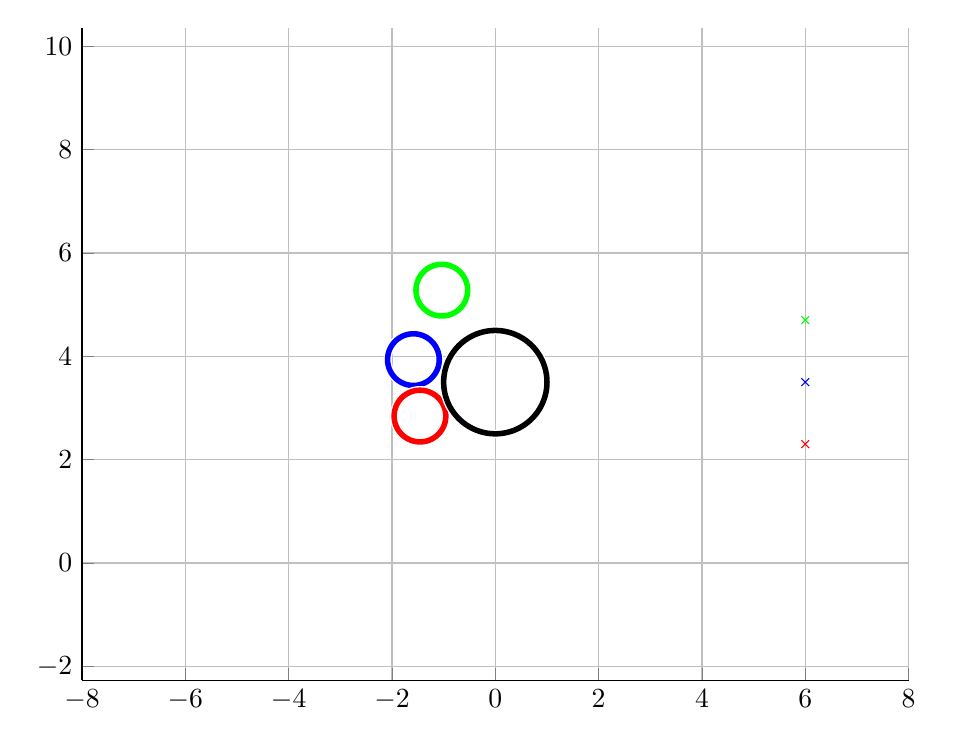
\begin{tikzpicture}

\begin{axis}[%
width=4.133in,
height=3.26in,
at={(0.693in,0.44in)},
scale only axis,
unbounded coords=jump,
xmin=-8,
xmax=8,
xmajorgrids,
ymin=-2.26954236044553,
ymax=10.3498124782641,
ymajorgrids,
axis background/.style={fill=white},
axis x line*=bottom,
axis y line*=left
]
\addplot [color=blue,only marks,mark=x,mark options={solid},forget plot]
  table[row sep=crcr]{%
6	3.5\\
};
\addplot [color=red,only marks,mark=x,mark options={solid},forget plot]
  table[row sep=crcr]{%
6	2.3\\
};
\addplot [color=green,only marks,mark=x,mark options={solid},forget plot]
  table[row sep=crcr]{%
6	4.7\\
};
\addplot [color=white,solid,line width=3.0pt,forget plot]
  table[row sep=crcr]{%
-1.08553726964379	3.93571674789681\\
-1.08584185613424	3.95316649624806\\
-1.08675524451388	3.97059498476887\\
-1.08827632195965	3.98798097953064\\
-1.09040323527301	4.00530329837684\\
-1.09313339313769	4.02254083673028\\
-1.09646346927689	4.03967259330569\\
-1.10038940650579	4.05667769569664\\
-1.10490642167463	4.07353542580531\\
-1.11000901149621	4.09022524508428\\
-1.11569095925084	4.10672681955965\\
-1.1219453423604	4.12302004460477\\
-1.12876454082249	4.13908506943471\\
-1.13614024649421	4.15490232129135\\
-1.14406347321433	4.17045252928976\\
-1.15252456775157	4.18571674789681\\
-1.16151322156558	4.20067638001341\\
-1.17101848336627	4.21531319963218\\
-1.18102877245632	4.22960937404305\\
-1.19153189284043	4.24354748555964\\
-1.2025150480843	4.25711055274008\\
-1.21396485690509	4.27028205107624\\
-1.22586736947447	4.28304593312631\\
-1.23820808441429	4.29538664806614\\
-1.25097196646436	4.30728916063551\\
-1.26414346480052	4.3187389694563\\
-1.27770653198096	4.32972212470017\\
-1.29164464349755	4.34022524508428\\
-1.30594081790842	4.35023553417433\\
-1.32057763752719	4.35974079597502\\
-1.33553726964379	4.36872944978903\\
-1.35080148825085	4.37719054432627\\
-1.36635169624925	4.38511377104639\\
-1.38216894810589	4.39248947671811\\
-1.39823397293584	4.3993086751802\\
-1.41452719798096	4.40556305828976\\
-1.43102877245632	4.41124500604439\\
-1.44771859173529	4.41634759586597\\
-1.46457632184396	4.42086461103481\\
-1.48158142423491	4.42479054826371\\
-1.49871318081033	4.42812062440291\\
-1.51595071916376	4.4308507822676\\
-1.53327303800996	4.43297769558095\\
-1.55065903277173	4.43449877302672\\
-1.56808752129254	4.43541216140636\\
-1.58553726964379	4.43571674789681\\
-1.60298701799504	4.43541216140636\\
-1.62041550651585	4.43449877302672\\
-1.63780150127762	4.43297769558095\\
-1.65512382012382	4.4308507822676\\
-1.67236135847726	4.42812062440291\\
-1.68949311505267	4.42479054826371\\
-1.70649821744363	4.42086461103481\\
-1.72335594755229	4.41634759586597\\
-1.74004576683126	4.41124500604439\\
-1.75654734130663	4.40556305828976\\
-1.77284056635175	4.3993086751802\\
-1.78890559118169	4.39248947671811\\
-1.80472284303833	4.38511377104639\\
-1.82027305103674	4.37719054432627\\
-1.83553726964379	4.36872944978903\\
-1.85049690176039	4.35974079597502\\
-1.86513372137916	4.35023553417433\\
-1.87942989579003	4.34022524508428\\
-1.89336800730662	4.32972212470017\\
-1.90693107448706	4.3187389694563\\
-1.92010257282322	4.30728916063551\\
-1.93286645487329	4.29538664806614\\
-1.94520716981312	4.28304593312631\\
-1.95710968238249	4.27028205107624\\
-1.96855949120328	4.25711055274008\\
-1.97954264644715	4.24354748555964\\
-1.99004576683126	4.22960937404305\\
-2.00005605592131	4.21531319963218\\
-2.009561317722	4.20067638001341\\
-2.01854997153601	4.18571674789681\\
-2.02701106607325	4.17045252928976\\
-2.03493429279337	4.15490232129135\\
-2.04230999846509	4.13908506943471\\
-2.04912919692718	4.12302004460477\\
-2.05538358003675	4.10672681955965\\
-2.06106552779137	4.09022524508428\\
-2.06616811761295	4.07353542580531\\
-2.07068513278179	4.05667769569664\\
-2.07461107001069	4.03967259330569\\
-2.0779411461499	4.02254083673028\\
-2.08067130401458	4.00530329837684\\
-2.08279821732793	3.98798097953064\\
-2.0843192947737	3.97059498476887\\
-2.08523268315334	3.95316649624806\\
-2.08553726964379	3.93571674789681\\
-2.08523268315334	3.91826699954556\\
-2.0843192947737	3.90083851102475\\
-2.08279821732793	3.88345251626298\\
-2.08067130401458	3.86613019741678\\
-2.0779411461499	3.84889265906335\\
-2.07461107001069	3.83176090248793\\
-2.07068513278179	3.81475580009698\\
-2.06616811761295	3.79789806998831\\
-2.06106552779137	3.78120825070934\\
-2.05538358003675	3.76470667623398\\
-2.04912919692718	3.74841345118885\\
-2.04230999846509	3.73234842635891\\
-2.03493429279337	3.71653117450227\\
-2.02701106607325	3.70098096650386\\
-2.01854997153601	3.68571674789681\\
-2.009561317722	3.67075711578021\\
-2.00005605592131	3.65612029616144\\
-1.99004576683126	3.64182412175057\\
-1.97954264644715	3.62788601023398\\
-1.96855949120328	3.61432294305354\\
-1.95710968238249	3.60115144471738\\
-1.94520716981312	3.58838756266731\\
-1.93286645487329	3.57604684772748\\
-1.92010257282322	3.56414433515811\\
-1.90693107448706	3.55269452633732\\
-1.89336800730662	3.54171137109345\\
-1.87942989579003	3.53120825070934\\
-1.86513372137916	3.52119796161929\\
-1.85049690176039	3.5116926998186\\
-1.83553726964379	3.50270404600459\\
-1.82027305103674	3.49424295146735\\
-1.80472284303833	3.48631972474723\\
-1.78890559118169	3.47894401907551\\
-1.77284056635175	3.47212482061342\\
-1.75654734130663	3.46587043750386\\
-1.74004576683126	3.46018848974923\\
-1.72335594755229	3.45508589992765\\
-1.70649821744363	3.45056888475881\\
-1.68949311505267	3.44664294752991\\
-1.67236135847726	3.44331287139071\\
-1.65512382012382	3.44058271352603\\
-1.63780150127762	3.43845580021267\\
-1.62041550651585	3.4369347227669\\
-1.60298701799504	3.43602133438726\\
-1.58553726964379	3.43571674789681\\
-1.56808752129254	3.43602133438726\\
-1.55065903277173	3.4369347227669\\
-1.53327303800996	3.43845580021267\\
-1.51595071916376	3.44058271352603\\
-1.49871318081033	3.44331287139071\\
-1.48158142423491	3.44664294752991\\
-1.46457632184396	3.45056888475881\\
-1.44771859173529	3.45508589992765\\
-1.43102877245632	3.46018848974923\\
-1.41452719798096	3.46587043750386\\
-1.39823397293584	3.47212482061342\\
-1.38216894810589	3.47894401907551\\
-1.36635169624925	3.48631972474723\\
-1.35080148825085	3.49424295146735\\
-1.33553726964379	3.50270404600459\\
-1.32057763752719	3.5116926998186\\
-1.30594081790842	3.52119796161929\\
-1.29164464349755	3.53120825070934\\
-1.27770653198096	3.54171137109345\\
-1.26414346480052	3.55269452633732\\
-1.25097196646436	3.56414433515811\\
-1.23820808441429	3.57604684772748\\
-1.22586736947447	3.58838756266731\\
-1.21396485690509	3.60115144471738\\
-1.2025150480843	3.61432294305354\\
-1.19153189284043	3.62788601023398\\
-1.18102877245632	3.64182412175057\\
-1.17101848336627	3.65612029616144\\
-1.16151322156558	3.67075711578021\\
-1.15252456775157	3.68571674789681\\
-1.14406347321433	3.70098096650386\\
-1.13614024649421	3.71653117450227\\
-1.12876454082249	3.73234842635891\\
-1.1219453423604	3.74841345118885\\
-1.11569095925084	3.76470667623398\\
-1.11000901149621	3.78120825070934\\
-1.10490642167463	3.79789806998831\\
-1.10038940650579	3.81475580009698\\
-1.09646346927689	3.83176090248793\\
-1.09313339313769	3.84889265906334\\
-1.09040323527301	3.86613019741678\\
-1.08827632195965	3.88345251626298\\
-1.08675524451388	3.90083851102475\\
-1.08584185613424	3.91826699954556\\
-1.08553726964379	3.93571674789681\\
nan	nan\\
};
\addplot [color=blue,solid,line width=2.0pt,forget plot]
  table[row sep=crcr]{%
-1.08553726964379	3.93571674789681\\
-1.08584185613424	3.95316649624806\\
-1.08675524451388	3.97059498476887\\
-1.08827632195965	3.98798097953064\\
-1.09040323527301	4.00530329837684\\
-1.09313339313769	4.02254083673028\\
-1.09646346927689	4.03967259330569\\
-1.10038940650579	4.05667769569664\\
-1.10490642167463	4.07353542580531\\
-1.11000901149621	4.09022524508428\\
-1.11569095925084	4.10672681955965\\
-1.1219453423604	4.12302004460477\\
-1.12876454082249	4.13908506943471\\
-1.13614024649421	4.15490232129135\\
-1.14406347321433	4.17045252928976\\
-1.15252456775157	4.18571674789681\\
-1.16151322156558	4.20067638001341\\
-1.17101848336627	4.21531319963218\\
-1.18102877245632	4.22960937404305\\
-1.19153189284043	4.24354748555964\\
-1.2025150480843	4.25711055274008\\
-1.21396485690509	4.27028205107624\\
-1.22586736947447	4.28304593312631\\
-1.23820808441429	4.29538664806614\\
-1.25097196646436	4.30728916063551\\
-1.26414346480052	4.3187389694563\\
-1.27770653198096	4.32972212470017\\
-1.29164464349755	4.34022524508428\\
-1.30594081790842	4.35023553417433\\
-1.32057763752719	4.35974079597502\\
-1.33553726964379	4.36872944978903\\
-1.35080148825085	4.37719054432627\\
-1.36635169624925	4.38511377104639\\
-1.38216894810589	4.39248947671811\\
-1.39823397293584	4.3993086751802\\
-1.41452719798096	4.40556305828976\\
-1.43102877245632	4.41124500604439\\
-1.44771859173529	4.41634759586597\\
-1.46457632184396	4.42086461103481\\
-1.48158142423491	4.42479054826371\\
-1.49871318081033	4.42812062440291\\
-1.51595071916376	4.4308507822676\\
-1.53327303800996	4.43297769558095\\
-1.55065903277173	4.43449877302672\\
-1.56808752129254	4.43541216140636\\
-1.58553726964379	4.43571674789681\\
-1.60298701799504	4.43541216140636\\
-1.62041550651585	4.43449877302672\\
-1.63780150127762	4.43297769558095\\
-1.65512382012382	4.4308507822676\\
-1.67236135847726	4.42812062440291\\
-1.68949311505267	4.42479054826371\\
-1.70649821744363	4.42086461103481\\
-1.72335594755229	4.41634759586597\\
-1.74004576683126	4.41124500604439\\
-1.75654734130663	4.40556305828976\\
-1.77284056635175	4.3993086751802\\
-1.78890559118169	4.39248947671811\\
-1.80472284303833	4.38511377104639\\
-1.82027305103674	4.37719054432627\\
-1.83553726964379	4.36872944978903\\
-1.85049690176039	4.35974079597502\\
-1.86513372137916	4.35023553417433\\
-1.87942989579003	4.34022524508428\\
-1.89336800730662	4.32972212470017\\
-1.90693107448706	4.3187389694563\\
-1.92010257282322	4.30728916063551\\
-1.93286645487329	4.29538664806614\\
-1.94520716981312	4.28304593312631\\
-1.95710968238249	4.27028205107624\\
-1.96855949120328	4.25711055274008\\
-1.97954264644715	4.24354748555964\\
-1.99004576683126	4.22960937404305\\
-2.00005605592131	4.21531319963218\\
-2.009561317722	4.20067638001341\\
-2.01854997153601	4.18571674789681\\
-2.02701106607325	4.17045252928976\\
-2.03493429279337	4.15490232129135\\
-2.04230999846509	4.13908506943471\\
-2.04912919692718	4.12302004460477\\
-2.05538358003675	4.10672681955965\\
-2.06106552779137	4.09022524508428\\
-2.06616811761295	4.07353542580531\\
-2.07068513278179	4.05667769569664\\
-2.07461107001069	4.03967259330569\\
-2.0779411461499	4.02254083673028\\
-2.08067130401458	4.00530329837684\\
-2.08279821732793	3.98798097953064\\
-2.0843192947737	3.97059498476887\\
-2.08523268315334	3.95316649624806\\
-2.08553726964379	3.93571674789681\\
-2.08523268315334	3.91826699954556\\
-2.0843192947737	3.90083851102475\\
-2.08279821732793	3.88345251626298\\
-2.08067130401458	3.86613019741678\\
-2.0779411461499	3.84889265906335\\
-2.07461107001069	3.83176090248793\\
-2.07068513278179	3.81475580009698\\
-2.06616811761295	3.79789806998831\\
-2.06106552779137	3.78120825070934\\
-2.05538358003675	3.76470667623398\\
-2.04912919692718	3.74841345118885\\
-2.04230999846509	3.73234842635891\\
-2.03493429279337	3.71653117450227\\
-2.02701106607325	3.70098096650386\\
-2.01854997153601	3.68571674789681\\
-2.009561317722	3.67075711578021\\
-2.00005605592131	3.65612029616144\\
-1.99004576683126	3.64182412175057\\
-1.97954264644715	3.62788601023398\\
-1.96855949120328	3.61432294305354\\
-1.95710968238249	3.60115144471738\\
-1.94520716981312	3.58838756266731\\
-1.93286645487329	3.57604684772748\\
-1.92010257282322	3.56414433515811\\
-1.90693107448706	3.55269452633732\\
-1.89336800730662	3.54171137109345\\
-1.87942989579003	3.53120825070934\\
-1.86513372137916	3.52119796161929\\
-1.85049690176039	3.5116926998186\\
-1.83553726964379	3.50270404600459\\
-1.82027305103674	3.49424295146735\\
-1.80472284303833	3.48631972474723\\
-1.78890559118169	3.47894401907551\\
-1.77284056635175	3.47212482061342\\
-1.75654734130663	3.46587043750386\\
-1.74004576683126	3.46018848974923\\
-1.72335594755229	3.45508589992765\\
-1.70649821744363	3.45056888475881\\
-1.68949311505267	3.44664294752991\\
-1.67236135847726	3.44331287139071\\
-1.65512382012382	3.44058271352603\\
-1.63780150127762	3.43845580021267\\
-1.62041550651585	3.4369347227669\\
-1.60298701799504	3.43602133438726\\
-1.58553726964379	3.43571674789681\\
-1.56808752129254	3.43602133438726\\
-1.55065903277173	3.4369347227669\\
-1.53327303800996	3.43845580021267\\
-1.51595071916376	3.44058271352603\\
-1.49871318081033	3.44331287139071\\
-1.48158142423491	3.44664294752991\\
-1.46457632184396	3.45056888475881\\
-1.44771859173529	3.45508589992765\\
-1.43102877245632	3.46018848974923\\
-1.41452719798096	3.46587043750386\\
-1.39823397293584	3.47212482061342\\
-1.38216894810589	3.47894401907551\\
-1.36635169624925	3.48631972474723\\
-1.35080148825085	3.49424295146735\\
-1.33553726964379	3.50270404600459\\
-1.32057763752719	3.5116926998186\\
-1.30594081790842	3.52119796161929\\
-1.29164464349755	3.53120825070934\\
-1.27770653198096	3.54171137109345\\
-1.26414346480052	3.55269452633732\\
-1.25097196646436	3.56414433515811\\
-1.23820808441429	3.57604684772748\\
-1.22586736947447	3.58838756266731\\
-1.21396485690509	3.60115144471738\\
-1.2025150480843	3.61432294305354\\
-1.19153189284043	3.62788601023398\\
-1.18102877245632	3.64182412175057\\
-1.17101848336627	3.65612029616144\\
-1.16151322156558	3.67075711578021\\
-1.15252456775157	3.68571674789681\\
-1.14406347321433	3.70098096650386\\
-1.13614024649421	3.71653117450227\\
-1.12876454082249	3.73234842635891\\
-1.1219453423604	3.74841345118885\\
-1.11569095925084	3.76470667623398\\
-1.11000901149621	3.78120825070934\\
-1.10490642167463	3.79789806998831\\
-1.10038940650579	3.81475580009698\\
-1.09646346927689	3.83176090248793\\
-1.09313339313769	3.84889265906334\\
-1.09040323527301	3.86613019741678\\
-1.08827632195965	3.88345251626298\\
-1.08675524451388	3.90083851102475\\
-1.08584185613424	3.91826699954556\\
-1.08553726964379	3.93571674789681\\
nan	nan\\
};
\addplot [color=white,solid,line width=3.0pt,forget plot]
  table[row sep=crcr]{%
-0.958900653726882	2.84303053148771\\
-0.959205240217334	2.86048027983896\\
-0.96011862859697	2.87790876835977\\
-0.961639706042746	2.89529476312154\\
-0.963766619356097	2.91261708196774\\
-0.966496777220778	2.92985462032118\\
-0.969826853359979	2.94698637689659\\
-0.973752790588884	2.96399147928754\\
-0.978269805757723	2.98084920939621\\
-0.983372395579305	2.99753902867518\\
-0.989054343333928	3.01404060315054\\
-0.995308726443489	3.03033382819567\\
-1.00212792490558	3.04639885302561\\
-1.0095036305773	3.06221610488225\\
-1.01742685729742	3.07776631288066\\
-1.02588795183466	3.09303053148771\\
-1.03487660564867	3.10799016360431\\
-1.04438186744936	3.12262698322308\\
-1.05439215653941	3.13692315763395\\
-1.06489527692352	3.15086126915054\\
-1.07587843216739	3.16442433633098\\
-1.08732824098819	3.17759583466714\\
-1.09923075355756	3.19035971671721\\
-1.11157146849738	3.20270043165704\\
-1.12433535054745	3.21460294422641\\
-1.13750684888361	3.2260527530472\\
-1.15106991606405	3.23703590829107\\
-1.16500802758065	3.24753902867518\\
-1.17930420199151	3.25754931776523\\
-1.19394102161028	3.26705457956592\\
-1.20890065372688	3.27604323337993\\
-1.22416487233394	3.28450432791717\\
-1.23971508033234	3.29242755463729\\
-1.25553233218898	3.29980326030901\\
-1.27159735701893	3.3066224587711\\
-1.28789058206405	3.31287684188066\\
-1.30439215653941	3.31855878963529\\
-1.32108197581838	3.32366137945687\\
-1.33793970592705	3.32817839462571\\
-1.354944808318	3.33210433185461\\
-1.37207656489342	3.33543440799381\\
-1.38931410324685	3.3381645658585\\
-1.40663642209306	3.34029147917185\\
-1.42402241685482	3.34181255661762\\
-1.44145090537563	3.34272594499726\\
-1.45890065372688	3.34303053148771\\
-1.47635040207813	3.34272594499726\\
-1.49377889059894	3.34181255661762\\
-1.51116488536071	3.34029147917185\\
-1.52848720420691	3.3381645658585\\
-1.54572474256035	3.33543440799381\\
-1.56285649913576	3.33210433185461\\
-1.57986160152672	3.32817839462571\\
-1.59671933163538	3.32366137945687\\
-1.61340915091436	3.31855878963529\\
-1.62991072538972	3.31287684188066\\
-1.64620395043484	3.3066224587711\\
-1.66226897526478	3.29980326030901\\
-1.67808622712142	3.29242755463729\\
-1.69363643511983	3.28450432791717\\
-1.70890065372688	3.27604323337993\\
-1.72386028584348	3.26705457956592\\
-1.73849710546226	3.25754931776523\\
-1.75279327987312	3.24753902867518\\
-1.76673139138971	3.23703590829107\\
-1.78029445857015	3.2260527530472\\
-1.79346595690631	3.21460294422641\\
-1.80622983895638	3.20270043165704\\
-1.81857055389621	3.19035971671721\\
-1.83047306646558	3.17759583466714\\
-1.84192287528637	3.16442433633098\\
-1.85290603053024	3.15086126915054\\
-1.86340915091436	3.13692315763395\\
-1.8734194400044	3.12262698322308\\
-1.8829247018051	3.10799016360431\\
-1.8919133556191	3.09303053148771\\
-1.90037445015635	3.07776631288066\\
-1.90829767687647	3.06221610488225\\
-1.91567338254818	3.04639885302561\\
-1.92249258101028	3.03033382819567\\
-1.92874696411984	3.01404060315054\\
-1.93442891187446	2.99753902867518\\
-1.93953150169604	2.98084920939621\\
-1.94404851686488	2.96399147928754\\
-1.94797445409379	2.94698637689659\\
-1.95130453023299	2.92985462032118\\
-1.95403468809767	2.91261708196774\\
-1.95616160141102	2.89529476312154\\
-1.95768267885679	2.87790876835977\\
-1.95859606723643	2.86048027983896\\
-1.95890065372688	2.84303053148771\\
-1.95859606723643	2.82558078313646\\
-1.95768267885679	2.80815229461565\\
-1.95616160141102	2.79076629985388\\
-1.95403468809767	2.77344398100768\\
-1.95130453023299	2.75620644265424\\
-1.94797445409379	2.73907468607883\\
-1.94404851686488	2.72206958368788\\
-1.93953150169604	2.70521185357921\\
-1.93442891187446	2.68852203430024\\
-1.92874696411984	2.67202045982488\\
-1.92249258101028	2.65572723477975\\
-1.91567338254818	2.63966220994981\\
-1.90829767687647	2.62384495809317\\
-1.90037445015635	2.60829475009476\\
-1.8919133556191	2.59303053148771\\
-1.8829247018051	2.57807089937111\\
-1.8734194400044	2.56343407975234\\
-1.86340915091436	2.54913790534147\\
-1.85290603053024	2.53519979382488\\
-1.84192287528637	2.52163672664444\\
-1.83047306646558	2.50846522830828\\
-1.81857055389621	2.49570134625821\\
-1.80622983895638	2.48336063131838\\
-1.79346595690631	2.47145811874901\\
-1.78029445857015	2.46000830992822\\
-1.76673139138971	2.44902515468435\\
-1.75279327987312	2.43852203430024\\
-1.73849710546226	2.42851174521019\\
-1.72386028584348	2.4190064834095\\
-1.70890065372688	2.41001782959549\\
-1.69363643511983	2.40155673505825\\
-1.67808622712142	2.39363350833813\\
-1.66226897526478	2.38625780266641\\
-1.64620395043484	2.37943860420432\\
-1.62991072538972	2.37318422109476\\
-1.61340915091436	2.36750227334013\\
-1.59671933163538	2.36239968351855\\
-1.57986160152672	2.35788266834971\\
-1.56285649913576	2.35395673112081\\
-1.54572474256035	2.35062665498161\\
-1.52848720420691	2.34789649711692\\
-1.51116488536071	2.34576958380357\\
-1.49377889059895	2.3442485063578\\
-1.47635040207813	2.34333511797816\\
-1.45890065372688	2.34303053148771\\
-1.44145090537563	2.34333511797816\\
-1.42402241685482	2.3442485063578\\
-1.40663642209306	2.34576958380357\\
-1.38931410324685	2.34789649711692\\
-1.37207656489342	2.35062665498161\\
-1.354944808318	2.35395673112081\\
-1.33793970592705	2.35788266834971\\
-1.32108197581838	2.36239968351855\\
-1.30439215653941	2.36750227334013\\
-1.28789058206405	2.37318422109476\\
-1.27159735701893	2.37943860420432\\
-1.25553233218898	2.38625780266641\\
-1.23971508033234	2.39363350833813\\
-1.22416487233394	2.40155673505825\\
-1.20890065372688	2.41001782959549\\
-1.19394102161028	2.4190064834095\\
-1.17930420199151	2.42851174521019\\
-1.16500802758065	2.43852203430024\\
-1.15106991606405	2.44902515468435\\
-1.13750684888361	2.46000830992822\\
-1.12433535054745	2.47145811874901\\
-1.11157146849738	2.48336063131838\\
-1.09923075355756	2.49570134625821\\
-1.08732824098819	2.50846522830828\\
-1.07587843216739	2.52163672664444\\
-1.06489527692352	2.53519979382488\\
-1.05439215653941	2.54913790534147\\
-1.04438186744936	2.56343407975234\\
-1.03487660564867	2.57807089937111\\
-1.02588795183466	2.59303053148771\\
-1.01742685729742	2.60829475009476\\
-1.0095036305773	2.62384495809317\\
-1.00212792490558	2.63966220994981\\
-0.995308726443489	2.65572723477975\\
-0.989054343333928	2.67202045982488\\
-0.983372395579305	2.68852203430024\\
-0.978269805757723	2.70521185357921\\
-0.973752790588884	2.72206958368788\\
-0.969826853359979	2.73907468607883\\
-0.966496777220778	2.75620644265424\\
-0.963766619356097	2.77344398100768\\
-0.961639706042746	2.79076629985388\\
-0.96011862859697	2.80815229461565\\
-0.959205240217334	2.82558078313646\\
-0.958900653726882	2.84303053148771\\
nan	nan\\
};
\addplot [color=red,solid,line width=2.0pt,forget plot]
  table[row sep=crcr]{%
-0.958900653726882	2.84303053148771\\
-0.959205240217334	2.86048027983896\\
-0.96011862859697	2.87790876835977\\
-0.961639706042746	2.89529476312154\\
-0.963766619356097	2.91261708196774\\
-0.966496777220778	2.92985462032118\\
-0.969826853359979	2.94698637689659\\
-0.973752790588884	2.96399147928754\\
-0.978269805757723	2.98084920939621\\
-0.983372395579305	2.99753902867518\\
-0.989054343333928	3.01404060315054\\
-0.995308726443489	3.03033382819567\\
-1.00212792490558	3.04639885302561\\
-1.0095036305773	3.06221610488225\\
-1.01742685729742	3.07776631288066\\
-1.02588795183466	3.09303053148771\\
-1.03487660564867	3.10799016360431\\
-1.04438186744936	3.12262698322308\\
-1.05439215653941	3.13692315763395\\
-1.06489527692352	3.15086126915054\\
-1.07587843216739	3.16442433633098\\
-1.08732824098819	3.17759583466714\\
-1.09923075355756	3.19035971671721\\
-1.11157146849738	3.20270043165704\\
-1.12433535054745	3.21460294422641\\
-1.13750684888361	3.2260527530472\\
-1.15106991606405	3.23703590829107\\
-1.16500802758065	3.24753902867518\\
-1.17930420199151	3.25754931776523\\
-1.19394102161028	3.26705457956592\\
-1.20890065372688	3.27604323337993\\
-1.22416487233394	3.28450432791717\\
-1.23971508033234	3.29242755463729\\
-1.25553233218898	3.29980326030901\\
-1.27159735701893	3.3066224587711\\
-1.28789058206405	3.31287684188066\\
-1.30439215653941	3.31855878963529\\
-1.32108197581838	3.32366137945687\\
-1.33793970592705	3.32817839462571\\
-1.354944808318	3.33210433185461\\
-1.37207656489342	3.33543440799381\\
-1.38931410324685	3.3381645658585\\
-1.40663642209306	3.34029147917185\\
-1.42402241685482	3.34181255661762\\
-1.44145090537563	3.34272594499726\\
-1.45890065372688	3.34303053148771\\
-1.47635040207813	3.34272594499726\\
-1.49377889059894	3.34181255661762\\
-1.51116488536071	3.34029147917185\\
-1.52848720420691	3.3381645658585\\
-1.54572474256035	3.33543440799381\\
-1.56285649913576	3.33210433185461\\
-1.57986160152672	3.32817839462571\\
-1.59671933163538	3.32366137945687\\
-1.61340915091436	3.31855878963529\\
-1.62991072538972	3.31287684188066\\
-1.64620395043484	3.3066224587711\\
-1.66226897526478	3.29980326030901\\
-1.67808622712142	3.29242755463729\\
-1.69363643511983	3.28450432791717\\
-1.70890065372688	3.27604323337993\\
-1.72386028584348	3.26705457956592\\
-1.73849710546226	3.25754931776523\\
-1.75279327987312	3.24753902867518\\
-1.76673139138971	3.23703590829107\\
-1.78029445857015	3.2260527530472\\
-1.79346595690631	3.21460294422641\\
-1.80622983895638	3.20270043165704\\
-1.81857055389621	3.19035971671721\\
-1.83047306646558	3.17759583466714\\
-1.84192287528637	3.16442433633098\\
-1.85290603053024	3.15086126915054\\
-1.86340915091436	3.13692315763395\\
-1.8734194400044	3.12262698322308\\
-1.8829247018051	3.10799016360431\\
-1.8919133556191	3.09303053148771\\
-1.90037445015635	3.07776631288066\\
-1.90829767687647	3.06221610488225\\
-1.91567338254818	3.04639885302561\\
-1.92249258101028	3.03033382819567\\
-1.92874696411984	3.01404060315054\\
-1.93442891187446	2.99753902867518\\
-1.93953150169604	2.98084920939621\\
-1.94404851686488	2.96399147928754\\
-1.94797445409379	2.94698637689659\\
-1.95130453023299	2.92985462032118\\
-1.95403468809767	2.91261708196774\\
-1.95616160141102	2.89529476312154\\
-1.95768267885679	2.87790876835977\\
-1.95859606723643	2.86048027983896\\
-1.95890065372688	2.84303053148771\\
-1.95859606723643	2.82558078313646\\
-1.95768267885679	2.80815229461565\\
-1.95616160141102	2.79076629985388\\
-1.95403468809767	2.77344398100768\\
-1.95130453023299	2.75620644265424\\
-1.94797445409379	2.73907468607883\\
-1.94404851686488	2.72206958368788\\
-1.93953150169604	2.70521185357921\\
-1.93442891187446	2.68852203430024\\
-1.92874696411984	2.67202045982488\\
-1.92249258101028	2.65572723477975\\
-1.91567338254818	2.63966220994981\\
-1.90829767687647	2.62384495809317\\
-1.90037445015635	2.60829475009476\\
-1.8919133556191	2.59303053148771\\
-1.8829247018051	2.57807089937111\\
-1.8734194400044	2.56343407975234\\
-1.86340915091436	2.54913790534147\\
-1.85290603053024	2.53519979382488\\
-1.84192287528637	2.52163672664444\\
-1.83047306646558	2.50846522830828\\
-1.81857055389621	2.49570134625821\\
-1.80622983895638	2.48336063131838\\
-1.79346595690631	2.47145811874901\\
-1.78029445857015	2.46000830992822\\
-1.76673139138971	2.44902515468435\\
-1.75279327987312	2.43852203430024\\
-1.73849710546226	2.42851174521019\\
-1.72386028584348	2.4190064834095\\
-1.70890065372688	2.41001782959549\\
-1.69363643511983	2.40155673505825\\
-1.67808622712142	2.39363350833813\\
-1.66226897526478	2.38625780266641\\
-1.64620395043484	2.37943860420432\\
-1.62991072538972	2.37318422109476\\
-1.61340915091436	2.36750227334013\\
-1.59671933163538	2.36239968351855\\
-1.57986160152672	2.35788266834971\\
-1.56285649913576	2.35395673112081\\
-1.54572474256035	2.35062665498161\\
-1.52848720420691	2.34789649711692\\
-1.51116488536071	2.34576958380357\\
-1.49377889059895	2.3442485063578\\
-1.47635040207813	2.34333511797816\\
-1.45890065372688	2.34303053148771\\
-1.44145090537563	2.34333511797816\\
-1.42402241685482	2.3442485063578\\
-1.40663642209306	2.34576958380357\\
-1.38931410324685	2.34789649711692\\
-1.37207656489342	2.35062665498161\\
-1.354944808318	2.35395673112081\\
-1.33793970592705	2.35788266834971\\
-1.32108197581838	2.36239968351855\\
-1.30439215653941	2.36750227334013\\
-1.28789058206405	2.37318422109476\\
-1.27159735701893	2.37943860420432\\
-1.25553233218898	2.38625780266641\\
-1.23971508033234	2.39363350833813\\
-1.22416487233394	2.40155673505825\\
-1.20890065372688	2.41001782959549\\
-1.19394102161028	2.4190064834095\\
-1.17930420199151	2.42851174521019\\
-1.16500802758065	2.43852203430024\\
-1.15106991606405	2.44902515468435\\
-1.13750684888361	2.46000830992822\\
-1.12433535054745	2.47145811874901\\
-1.11157146849738	2.48336063131838\\
-1.09923075355756	2.49570134625821\\
-1.08732824098819	2.50846522830828\\
-1.07587843216739	2.52163672664444\\
-1.06489527692352	2.53519979382488\\
-1.05439215653941	2.54913790534147\\
-1.04438186744936	2.56343407975234\\
-1.03487660564867	2.57807089937111\\
-1.02588795183466	2.59303053148771\\
-1.01742685729742	2.60829475009476\\
-1.0095036305773	2.62384495809317\\
-1.00212792490558	2.63966220994981\\
-0.995308726443489	2.65572723477975\\
-0.989054343333928	2.67202045982488\\
-0.983372395579305	2.68852203430024\\
-0.978269805757723	2.70521185357921\\
-0.973752790588884	2.72206958368788\\
-0.969826853359979	2.73907468607883\\
-0.966496777220778	2.75620644265424\\
-0.963766619356097	2.77344398100768\\
-0.961639706042746	2.79076629985388\\
-0.96011862859697	2.80815229461565\\
-0.959205240217334	2.82558078313646\\
-0.958900653726882	2.84303053148771\\
nan	nan\\
};
\addplot [color=white,solid,line width=3.0pt,forget plot]
  table[row sep=crcr]{%
-0.535822686189015	5.28027011781862\\
-0.536127272679467	5.29771986616987\\
-0.537040661059103	5.31514835469068\\
-0.538561738504879	5.33253434945245\\
-0.54068865181823	5.34985666829865\\
-0.543418809682911	5.36709420665208\\
-0.546748885822113	5.3842259632275\\
-0.550674823051017	5.40123106561845\\
-0.555191838219856	5.41808879572712\\
-0.560294428041439	5.43477861500609\\
-0.565976375796061	5.45128018948145\\
-0.572230758905622	5.46757341452657\\
-0.579049957367715	5.48363843935652\\
-0.586425663039432	5.49945569121316\\
-0.594348889759552	5.51500589921156\\
-0.602809984296796	5.53027011781862\\
-0.611798638110802	5.54522974993522\\
-0.621303899911495	5.55986656955399\\
-0.631314189001542	5.57416274396486\\
-0.641817309385654	5.58810085548145\\
-0.652800464629526	5.60166392266189\\
-0.664250273450318	5.61483542099805\\
-0.67615278601969	5.62759930304812\\
-0.688493500959517	5.63994001798794\\
-0.701257383009586	5.65184253055732\\
-0.714428881345746	5.66329233937811\\
-0.727991948526186	5.67427549462198\\
-0.741930060042779	5.68477861500609\\
-0.756226234453642	5.69478890409614\\
-0.770863054072413	5.70429416589683\\
-0.785822686189015	5.71328281971084\\
-0.80108690479607	5.72174391424808\\
-0.816637112794477	5.7296671409682\\
-0.832454364651115	5.73704284663992\\
-0.848519389481059	5.74386204510201\\
-0.864812614526181	5.75011642821157\\
-0.881314189001542	5.7557983759662\\
-0.898004008280516	5.76090096578778\\
-0.914861738389182	5.76541798095662\\
-0.931866840780136	5.76934391818552\\
-0.94899859735555	5.77267399432472\\
-0.966236135708983	5.7754041521894\\
-0.983558454555189	5.77753106550275\\
-1.00094444931695	5.77905214294853\\
-1.01837293783776	5.77996553132817\\
-1.03582268618902	5.78027011781862\\
-1.05327243454027	5.77996553132817\\
-1.07070092306108	5.77905214294853\\
-1.08808691782284	5.77753106550275\\
-1.10540923666905	5.7754041521894\\
-1.12264677502248	5.77267399432472\\
-1.13977853159789	5.76934391818552\\
-1.15678363398885	5.76541798095662\\
-1.17364136409751	5.76090096578778\\
-1.19033118337649	5.7557983759662\\
-1.20683275785185	5.75011642821157\\
-1.22312598289697	5.74386204510201\\
-1.23919100772692	5.73704284663992\\
-1.25500825958355	5.7296671409682\\
-1.27055846758196	5.72174391424808\\
-1.28582268618902	5.71328281971084\\
-1.30078231830562	5.70429416589683\\
-1.31541913792439	5.69478890409614\\
-1.32971531233525	5.68477861500609\\
-1.34365342385184	5.67427549462198\\
-1.35721649103229	5.66329233937811\\
-1.37038798936844	5.65184253055732\\
-1.38315187141851	5.63994001798794\\
-1.39549258635834	5.62759930304812\\
-1.40739509892771	5.61483542099805\\
-1.4188449077485	5.60166392266189\\
-1.42982806299238	5.58810085548145\\
-1.44033118337649	5.57416274396486\\
-1.45034147246654	5.55986656955399\\
-1.45984673426723	5.54522974993522\\
-1.46883538808123	5.53027011781862\\
-1.47729648261848	5.51500589921156\\
-1.4852197093386	5.49945569121316\\
-1.49259541501032	5.48363843935652\\
-1.49941461347241	5.46757341452657\\
-1.50566899658197	5.45128018948145\\
-1.51135094433659	5.43477861500609\\
-1.51645353415817	5.41808879572712\\
-1.52097054932701	5.40123106561845\\
-1.52489648655592	5.3842259632275\\
-1.52822656269512	5.36709420665208\\
-1.5309567205598	5.34985666829865\\
-1.53308363387315	5.33253434945245\\
-1.53460471131893	5.31514835469068\\
-1.53551809969856	5.29771986616987\\
-1.53582268618902	5.28027011781862\\
-1.53551809969856	5.26282036946737\\
-1.53460471131893	5.24539188094656\\
-1.53308363387315	5.22800588618479\\
-1.5309567205598	5.21068356733859\\
-1.52822656269512	5.19344602898515\\
-1.52489648655592	5.17631427240974\\
-1.52097054932701	5.15930917001879\\
-1.51645353415817	5.14245143991012\\
-1.51135094433659	5.12576162063114\\
-1.50566899658197	5.10926004615578\\
-1.49941461347241	5.09296682111066\\
-1.49259541501032	5.07690179628072\\
-1.4852197093386	5.06108454442408\\
-1.47729648261848	5.04553433642567\\
-1.46883538808123	5.03027011781862\\
-1.45984673426723	5.01531048570202\\
-1.45034147246654	5.00067366608325\\
-1.44033118337649	4.98637749167238\\
-1.42982806299238	4.97243938015579\\
-1.4188449077485	4.95887631297535\\
-1.40739509892771	4.94570481463919\\
-1.39549258635834	4.93294093258912\\
-1.38315187141851	4.92060021764929\\
-1.37038798936844	4.90869770507992\\
-1.35721649103229	4.89724789625913\\
-1.34365342385184	4.88626474101526\\
-1.32971531233525	4.87576162063115\\
-1.31541913792439	4.8657513315411\\
-1.30078231830562	4.85624606974041\\
-1.28582268618902	4.8472574159264\\
-1.27055846758196	4.83879632138916\\
-1.25500825958355	4.83087309466904\\
-1.23919100772692	4.82349738899732\\
-1.22312598289697	4.81667819053523\\
-1.20683275785185	4.81042380742566\\
-1.19033118337649	4.80474185967104\\
-1.17364136409751	4.79963926984946\\
-1.15678363398885	4.79512225468062\\
-1.1397785315979	4.79119631745172\\
-1.12264677502248	4.78786624131252\\
-1.10540923666905	4.78513608344783\\
-1.08808691782284	4.78300917013448\\
-1.07070092306108	4.78148809268871\\
-1.05327243454027	4.78057470430907\\
-1.03582268618902	4.78027011781862\\
-1.01837293783776	4.78057470430907\\
-1.00094444931695	4.78148809268871\\
-0.983558454555189	4.78300917013448\\
-0.966236135708983	4.78513608344783\\
-0.94899859735555	4.78786624131251\\
-0.931866840780136	4.79119631745172\\
-0.914861738389182	4.79512225468062\\
-0.898004008280516	4.79963926984946\\
-0.881314189001542	4.80474185967104\\
-0.864812614526181	4.81042380742566\\
-0.848519389481059	4.81667819053522\\
-0.832454364651115	4.82349738899732\\
-0.816637112794477	4.83087309466903\\
-0.80108690479607	4.83879632138915\\
-0.785822686189015	4.8472574159264\\
-0.770863054072413	4.85624606974041\\
-0.756226234453642	4.8657513315411\\
-0.741930060042779	4.87576162063114\\
-0.727991948526186	4.88626474101526\\
-0.714428881345746	4.89724789625913\\
-0.701257383009587	4.90869770507992\\
-0.688493500959517	4.92060021764929\\
-0.67615278601969	4.93294093258912\\
-0.664250273450318	4.94570481463919\\
-0.652800464629526	4.95887631297535\\
-0.641817309385655	4.97243938015579\\
-0.631314189001542	4.98637749167238\\
-0.621303899911495	5.00067366608325\\
-0.611798638110803	5.01531048570202\\
-0.602809984296796	5.03027011781862\\
-0.594348889759552	5.04553433642567\\
-0.586425663039432	5.06108454442408\\
-0.579049957367715	5.07690179628072\\
-0.572230758905622	5.09296682111066\\
-0.565976375796061	5.10926004615578\\
-0.560294428041439	5.12576162063114\\
-0.555191838219856	5.14245143991012\\
-0.550674823051017	5.15930917001878\\
-0.546748885822113	5.17631427240974\\
-0.543418809682911	5.19344602898515\\
-0.54068865181823	5.21068356733859\\
-0.538561738504879	5.22800588618479\\
-0.537040661059103	5.24539188094656\\
-0.536127272679467	5.26282036946737\\
-0.535822686189015	5.28027011781862\\
nan	nan\\
};
\addplot [color=green,solid,line width=2.0pt,forget plot]
  table[row sep=crcr]{%
-0.535822686189015	5.28027011781862\\
-0.536127272679467	5.29771986616987\\
-0.537040661059103	5.31514835469068\\
-0.538561738504879	5.33253434945245\\
-0.54068865181823	5.34985666829865\\
-0.543418809682911	5.36709420665208\\
-0.546748885822113	5.3842259632275\\
-0.550674823051017	5.40123106561845\\
-0.555191838219856	5.41808879572712\\
-0.560294428041439	5.43477861500609\\
-0.565976375796061	5.45128018948145\\
-0.572230758905622	5.46757341452657\\
-0.579049957367715	5.48363843935652\\
-0.586425663039432	5.49945569121316\\
-0.594348889759552	5.51500589921156\\
-0.602809984296796	5.53027011781862\\
-0.611798638110802	5.54522974993522\\
-0.621303899911495	5.55986656955399\\
-0.631314189001542	5.57416274396486\\
-0.641817309385654	5.58810085548145\\
-0.652800464629526	5.60166392266189\\
-0.664250273450318	5.61483542099805\\
-0.67615278601969	5.62759930304812\\
-0.688493500959517	5.63994001798794\\
-0.701257383009586	5.65184253055732\\
-0.714428881345746	5.66329233937811\\
-0.727991948526186	5.67427549462198\\
-0.741930060042779	5.68477861500609\\
-0.756226234453642	5.69478890409614\\
-0.770863054072413	5.70429416589683\\
-0.785822686189015	5.71328281971084\\
-0.80108690479607	5.72174391424808\\
-0.816637112794477	5.7296671409682\\
-0.832454364651115	5.73704284663992\\
-0.848519389481059	5.74386204510201\\
-0.864812614526181	5.75011642821157\\
-0.881314189001542	5.7557983759662\\
-0.898004008280516	5.76090096578778\\
-0.914861738389182	5.76541798095662\\
-0.931866840780136	5.76934391818552\\
-0.94899859735555	5.77267399432472\\
-0.966236135708983	5.7754041521894\\
-0.983558454555189	5.77753106550275\\
-1.00094444931695	5.77905214294853\\
-1.01837293783776	5.77996553132817\\
-1.03582268618902	5.78027011781862\\
-1.05327243454027	5.77996553132817\\
-1.07070092306108	5.77905214294853\\
-1.08808691782284	5.77753106550275\\
-1.10540923666905	5.7754041521894\\
-1.12264677502248	5.77267399432472\\
-1.13977853159789	5.76934391818552\\
-1.15678363398885	5.76541798095662\\
-1.17364136409751	5.76090096578778\\
-1.19033118337649	5.7557983759662\\
-1.20683275785185	5.75011642821157\\
-1.22312598289697	5.74386204510201\\
-1.23919100772692	5.73704284663992\\
-1.25500825958355	5.7296671409682\\
-1.27055846758196	5.72174391424808\\
-1.28582268618902	5.71328281971084\\
-1.30078231830562	5.70429416589683\\
-1.31541913792439	5.69478890409614\\
-1.32971531233525	5.68477861500609\\
-1.34365342385184	5.67427549462198\\
-1.35721649103229	5.66329233937811\\
-1.37038798936844	5.65184253055732\\
-1.38315187141851	5.63994001798794\\
-1.39549258635834	5.62759930304812\\
-1.40739509892771	5.61483542099805\\
-1.4188449077485	5.60166392266189\\
-1.42982806299238	5.58810085548145\\
-1.44033118337649	5.57416274396486\\
-1.45034147246654	5.55986656955399\\
-1.45984673426723	5.54522974993522\\
-1.46883538808123	5.53027011781862\\
-1.47729648261848	5.51500589921156\\
-1.4852197093386	5.49945569121316\\
-1.49259541501032	5.48363843935652\\
-1.49941461347241	5.46757341452657\\
-1.50566899658197	5.45128018948145\\
-1.51135094433659	5.43477861500609\\
-1.51645353415817	5.41808879572712\\
-1.52097054932701	5.40123106561845\\
-1.52489648655592	5.3842259632275\\
-1.52822656269512	5.36709420665208\\
-1.5309567205598	5.34985666829865\\
-1.53308363387315	5.33253434945245\\
-1.53460471131893	5.31514835469068\\
-1.53551809969856	5.29771986616987\\
-1.53582268618902	5.28027011781862\\
-1.53551809969856	5.26282036946737\\
-1.53460471131893	5.24539188094656\\
-1.53308363387315	5.22800588618479\\
-1.5309567205598	5.21068356733859\\
-1.52822656269512	5.19344602898515\\
-1.52489648655592	5.17631427240974\\
-1.52097054932701	5.15930917001879\\
-1.51645353415817	5.14245143991012\\
-1.51135094433659	5.12576162063114\\
-1.50566899658197	5.10926004615578\\
-1.49941461347241	5.09296682111066\\
-1.49259541501032	5.07690179628072\\
-1.4852197093386	5.06108454442408\\
-1.47729648261848	5.04553433642567\\
-1.46883538808123	5.03027011781862\\
-1.45984673426723	5.01531048570202\\
-1.45034147246654	5.00067366608325\\
-1.44033118337649	4.98637749167238\\
-1.42982806299238	4.97243938015579\\
-1.4188449077485	4.95887631297535\\
-1.40739509892771	4.94570481463919\\
-1.39549258635834	4.93294093258912\\
-1.38315187141851	4.92060021764929\\
-1.37038798936844	4.90869770507992\\
-1.35721649103229	4.89724789625913\\
-1.34365342385184	4.88626474101526\\
-1.32971531233525	4.87576162063115\\
-1.31541913792439	4.8657513315411\\
-1.30078231830562	4.85624606974041\\
-1.28582268618902	4.8472574159264\\
-1.27055846758196	4.83879632138916\\
-1.25500825958355	4.83087309466904\\
-1.23919100772692	4.82349738899732\\
-1.22312598289697	4.81667819053523\\
-1.20683275785185	4.81042380742566\\
-1.19033118337649	4.80474185967104\\
-1.17364136409751	4.79963926984946\\
-1.15678363398885	4.79512225468062\\
-1.1397785315979	4.79119631745172\\
-1.12264677502248	4.78786624131252\\
-1.10540923666905	4.78513608344783\\
-1.08808691782284	4.78300917013448\\
-1.07070092306108	4.78148809268871\\
-1.05327243454027	4.78057470430907\\
-1.03582268618902	4.78027011781862\\
-1.01837293783776	4.78057470430907\\
-1.00094444931695	4.78148809268871\\
-0.983558454555189	4.78300917013448\\
-0.966236135708983	4.78513608344783\\
-0.94899859735555	4.78786624131251\\
-0.931866840780136	4.79119631745172\\
-0.914861738389182	4.79512225468062\\
-0.898004008280516	4.79963926984946\\
-0.881314189001542	4.80474185967104\\
-0.864812614526181	4.81042380742566\\
-0.848519389481059	4.81667819053522\\
-0.832454364651115	4.82349738899732\\
-0.816637112794477	4.83087309466903\\
-0.80108690479607	4.83879632138915\\
-0.785822686189015	4.8472574159264\\
-0.770863054072413	4.85624606974041\\
-0.756226234453642	4.8657513315411\\
-0.741930060042779	4.87576162063114\\
-0.727991948526186	4.88626474101526\\
-0.714428881345746	4.89724789625913\\
-0.701257383009587	4.90869770507992\\
-0.688493500959517	4.92060021764929\\
-0.67615278601969	4.93294093258912\\
-0.664250273450318	4.94570481463919\\
-0.652800464629526	4.95887631297535\\
-0.641817309385655	4.97243938015579\\
-0.631314189001542	4.98637749167238\\
-0.621303899911495	5.00067366608325\\
-0.611798638110803	5.01531048570202\\
-0.602809984296796	5.03027011781862\\
-0.594348889759552	5.04553433642567\\
-0.586425663039432	5.06108454442408\\
-0.579049957367715	5.07690179628072\\
-0.572230758905622	5.09296682111066\\
-0.565976375796061	5.10926004615578\\
-0.560294428041439	5.12576162063114\\
-0.555191838219856	5.14245143991012\\
-0.550674823051017	5.15930917001878\\
-0.546748885822113	5.17631427240974\\
-0.543418809682911	5.19344602898515\\
-0.54068865181823	5.21068356733859\\
-0.538561738504879	5.22800588618479\\
-0.537040661059103	5.24539188094656\\
-0.536127272679467	5.26282036946737\\
-0.535822686189015	5.28027011781862\\
nan	nan\\
};
\addplot [color=white,solid,line width=3.0pt,forget plot]
  table[row sep=crcr]{%
1	3.5\\
0.999390827019096	3.5348994967025\\
0.997564050259824	3.56975647374413\\
0.994521895368273	3.60452846326765\\
0.99026806874157	3.63917310096007\\
0.984807753012208	3.67364817766693\\
0.978147600733806	3.70791169081776\\
0.970295726275996	3.74192189559967\\
0.961261695938319	3.775637355817\\
0.951056516295154	3.80901699437495\\
0.939692620785908	3.84202014332567\\
0.927183854566787	3.87460659341591\\
0.913545457642601	3.9067366430758\\
0.898794046299167	3.93837114678908\\
0.882947592858927	3.96947156278589\\
0.866025403784439	4\\
0.848048096156426	4.0299192642332\\
0.829037572555042	4.05919290347075\\
0.809016994374947	4.08778525229247\\
0.788010753606722	4.11566147532566\\
0.766044443118978	4.14278760968654\\
0.743144825477394	4.16913060635886\\
0.719339800338651	4.194658370459\\
0.694658370458997	4.21933980033865\\
0.669130606358858	4.24314482547739\\
0.642787609686539	4.26604444311898\\
0.615661475325658	4.28801075360672\\
0.587785252292473	4.30901699437495\\
0.559192903470747	4.32903757255504\\
0.529919264233205	4.34804809615643\\
0.5	4.36602540378444\\
0.469471562785891	4.38294759285893\\
0.438371146789077	4.39879404629917\\
0.4067366430758	4.4135454576426\\
0.374606593415912	4.42718385456679\\
0.342020143325669	4.43969262078591\\
0.309016994374947	4.45105651629515\\
0.275637355816999	4.46126169593832\\
0.241921895599668	4.470295726276\\
0.207911690817759	4.47814760073381\\
0.17364817766693	4.48480775301221\\
0.139173100960066	4.49026806874157\\
0.104528463267653	4.49452189536827\\
0.0697564737441255	4.49756405025982\\
0.0348994967025011	4.4993908270191\\
6.12323399573677e-17	4.5\\
-0.0348994967025007	4.4993908270191\\
-0.0697564737441253	4.49756405025982\\
-0.104528463267653	4.49452189536827\\
-0.139173100960065	4.49026806874157\\
-0.17364817766693	4.48480775301221\\
-0.207911690817759	4.47814760073381\\
-0.241921895599668	4.470295726276\\
-0.275637355816999	4.46126169593832\\
-0.309016994374947	4.45105651629515\\
-0.342020143325669	4.43969262078591\\
-0.374606593415912	4.42718385456679\\
-0.4067366430758	4.4135454576426\\
-0.438371146789078	4.39879404629917\\
-0.469471562785891	4.38294759285893\\
-0.5	4.36602540378444\\
-0.529919264233205	4.34804809615643\\
-0.559192903470747	4.32903757255504\\
-0.587785252292473	4.30901699437495\\
-0.615661475325658	4.28801075360672\\
-0.642787609686539	4.26604444311898\\
-0.669130606358858	4.24314482547739\\
-0.694658370458997	4.21933980033865\\
-0.719339800338651	4.194658370459\\
-0.743144825477394	4.16913060635886\\
-0.766044443118978	4.14278760968654\\
-0.788010753606722	4.11566147532566\\
-0.809016994374947	4.08778525229247\\
-0.829037572555042	4.05919290347075\\
-0.848048096156426	4.0299192642332\\
-0.866025403784439	4\\
-0.882947592858927	3.96947156278589\\
-0.898794046299167	3.93837114678908\\
-0.913545457642601	3.9067366430758\\
-0.927183854566787	3.87460659341591\\
-0.939692620785908	3.84202014332567\\
-0.951056516295154	3.80901699437495\\
-0.961261695938319	3.775637355817\\
-0.970295726275996	3.74192189559967\\
-0.978147600733806	3.70791169081776\\
-0.984807753012208	3.67364817766693\\
-0.99026806874157	3.63917310096007\\
-0.994521895368273	3.60452846326765\\
-0.997564050259824	3.56975647374413\\
-0.999390827019096	3.5348994967025\\
-1	3.5\\
-0.999390827019096	3.4651005032975\\
-0.997564050259824	3.43024352625588\\
-0.994521895368273	3.39547153673235\\
-0.99026806874157	3.36082689903993\\
-0.984807753012208	3.32635182233307\\
-0.978147600733806	3.29208830918224\\
-0.970295726275997	3.25807810440033\\
-0.961261695938319	3.224362644183\\
-0.951056516295154	3.19098300562505\\
-0.939692620785908	3.15797985667433\\
-0.927183854566787	3.12539340658409\\
-0.913545457642601	3.0932633569242\\
-0.898794046299167	3.06162885321092\\
-0.882947592858927	3.03052843721411\\
-0.866025403784439	3\\
-0.848048096156426	2.9700807357668\\
-0.829037572555042	2.94080709652925\\
-0.809016994374947	2.91221474770753\\
-0.788010753606722	2.88433852467434\\
-0.766044443118978	2.85721239031346\\
-0.743144825477394	2.83086939364114\\
-0.719339800338651	2.805341629541\\
-0.694658370458997	2.78066019966135\\
-0.669130606358858	2.75685517452261\\
-0.642787609686539	2.73395555688102\\
-0.615661475325658	2.71198924639328\\
-0.587785252292473	2.69098300562505\\
-0.559192903470747	2.67096242744496\\
-0.529919264233205	2.65195190384357\\
-0.5	2.63397459621556\\
-0.469471562785891	2.61705240714107\\
-0.438371146789078	2.60120595370083\\
-0.4067366430758	2.5864545423574\\
-0.374606593415912	2.57281614543321\\
-0.342020143325669	2.56030737921409\\
-0.309016994374948	2.54894348370485\\
-0.275637355816999	2.53873830406168\\
-0.241921895599668	2.529704273724\\
-0.20791169081776	2.52185239926619\\
-0.17364817766693	2.51519224698779\\
-0.139173100960065	2.50973193125843\\
-0.104528463267653	2.50547810463173\\
-0.0697564737441256	2.50243594974018\\
-0.0348994967025016	2.5006091729809\\
-1.83697019872103e-16	2.5\\
0.0348994967025013	2.5006091729809\\
0.0697564737441252	2.50243594974018\\
0.104528463267653	2.50547810463173\\
0.139173100960065	2.50973193125843\\
0.17364817766693	2.51519224698779\\
0.207911690817759	2.52185239926619\\
0.241921895599667	2.529704273724\\
0.275637355816999	2.53873830406168\\
0.309016994374947	2.54894348370485\\
0.342020143325668	2.56030737921409\\
0.374606593415912	2.57281614543321\\
0.406736643075801	2.5864545423574\\
0.438371146789077	2.60120595370083\\
0.46947156278589	2.61705240714107\\
0.5	2.63397459621556\\
0.529919264233205	2.65195190384357\\
0.559192903470746	2.67096242744496\\
0.587785252292473	2.69098300562505\\
0.615661475325659	2.71198924639328\\
0.642787609686539	2.73395555688102\\
0.669130606358858	2.75685517452261\\
0.694658370458997	2.78066019966135\\
0.719339800338651	2.805341629541\\
0.743144825477394	2.83086939364114\\
0.766044443118978	2.85721239031346\\
0.788010753606722	2.88433852467434\\
0.809016994374947	2.91221474770753\\
0.829037572555041	2.94080709652925\\
0.848048096156425	2.97008073576679\\
0.866025403784438	3\\
0.882947592858927	3.03052843721411\\
0.898794046299167	3.06162885321092\\
0.913545457642601	3.0932633569242\\
0.927183854566787	3.12539340658409\\
0.939692620785908	3.15797985667433\\
0.951056516295154	3.19098300562505\\
0.961261695938319	3.224362644183\\
0.970295726275996	3.25807810440033\\
0.978147600733806	3.29208830918224\\
0.984807753012208	3.32635182233307\\
0.99026806874157	3.36082689903993\\
0.994521895368273	3.39547153673235\\
0.997564050259824	3.43024352625588\\
0.999390827019096	3.4651005032975\\
1	3.5\\
nan	nan\\
};
\addplot [color=black,solid,line width=2.0pt,forget plot]
  table[row sep=crcr]{%
1	3.5\\
0.999390827019096	3.5348994967025\\
0.997564050259824	3.56975647374413\\
0.994521895368273	3.60452846326765\\
0.99026806874157	3.63917310096007\\
0.984807753012208	3.67364817766693\\
0.978147600733806	3.70791169081776\\
0.970295726275996	3.74192189559967\\
0.961261695938319	3.775637355817\\
0.951056516295154	3.80901699437495\\
0.939692620785908	3.84202014332567\\
0.927183854566787	3.87460659341591\\
0.913545457642601	3.9067366430758\\
0.898794046299167	3.93837114678908\\
0.882947592858927	3.96947156278589\\
0.866025403784439	4\\
0.848048096156426	4.0299192642332\\
0.829037572555042	4.05919290347075\\
0.809016994374947	4.08778525229247\\
0.788010753606722	4.11566147532566\\
0.766044443118978	4.14278760968654\\
0.743144825477394	4.16913060635886\\
0.719339800338651	4.194658370459\\
0.694658370458997	4.21933980033865\\
0.669130606358858	4.24314482547739\\
0.642787609686539	4.26604444311898\\
0.615661475325658	4.28801075360672\\
0.587785252292473	4.30901699437495\\
0.559192903470747	4.32903757255504\\
0.529919264233205	4.34804809615643\\
0.5	4.36602540378444\\
0.469471562785891	4.38294759285893\\
0.438371146789077	4.39879404629917\\
0.4067366430758	4.4135454576426\\
0.374606593415912	4.42718385456679\\
0.342020143325669	4.43969262078591\\
0.309016994374947	4.45105651629515\\
0.275637355816999	4.46126169593832\\
0.241921895599668	4.470295726276\\
0.207911690817759	4.47814760073381\\
0.17364817766693	4.48480775301221\\
0.139173100960066	4.49026806874157\\
0.104528463267653	4.49452189536827\\
0.0697564737441255	4.49756405025982\\
0.0348994967025011	4.4993908270191\\
6.12323399573677e-17	4.5\\
-0.0348994967025007	4.4993908270191\\
-0.0697564737441253	4.49756405025982\\
-0.104528463267653	4.49452189536827\\
-0.139173100960065	4.49026806874157\\
-0.17364817766693	4.48480775301221\\
-0.207911690817759	4.47814760073381\\
-0.241921895599668	4.470295726276\\
-0.275637355816999	4.46126169593832\\
-0.309016994374947	4.45105651629515\\
-0.342020143325669	4.43969262078591\\
-0.374606593415912	4.42718385456679\\
-0.4067366430758	4.4135454576426\\
-0.438371146789078	4.39879404629917\\
-0.469471562785891	4.38294759285893\\
-0.5	4.36602540378444\\
-0.529919264233205	4.34804809615643\\
-0.559192903470747	4.32903757255504\\
-0.587785252292473	4.30901699437495\\
-0.615661475325658	4.28801075360672\\
-0.642787609686539	4.26604444311898\\
-0.669130606358858	4.24314482547739\\
-0.694658370458997	4.21933980033865\\
-0.719339800338651	4.194658370459\\
-0.743144825477394	4.16913060635886\\
-0.766044443118978	4.14278760968654\\
-0.788010753606722	4.11566147532566\\
-0.809016994374947	4.08778525229247\\
-0.829037572555042	4.05919290347075\\
-0.848048096156426	4.0299192642332\\
-0.866025403784439	4\\
-0.882947592858927	3.96947156278589\\
-0.898794046299167	3.93837114678908\\
-0.913545457642601	3.9067366430758\\
-0.927183854566787	3.87460659341591\\
-0.939692620785908	3.84202014332567\\
-0.951056516295154	3.80901699437495\\
-0.961261695938319	3.775637355817\\
-0.970295726275996	3.74192189559967\\
-0.978147600733806	3.70791169081776\\
-0.984807753012208	3.67364817766693\\
-0.99026806874157	3.63917310096007\\
-0.994521895368273	3.60452846326765\\
-0.997564050259824	3.56975647374413\\
-0.999390827019096	3.5348994967025\\
-1	3.5\\
-0.999390827019096	3.4651005032975\\
-0.997564050259824	3.43024352625588\\
-0.994521895368273	3.39547153673235\\
-0.99026806874157	3.36082689903993\\
-0.984807753012208	3.32635182233307\\
-0.978147600733806	3.29208830918224\\
-0.970295726275997	3.25807810440033\\
-0.961261695938319	3.224362644183\\
-0.951056516295154	3.19098300562505\\
-0.939692620785908	3.15797985667433\\
-0.927183854566787	3.12539340658409\\
-0.913545457642601	3.0932633569242\\
-0.898794046299167	3.06162885321092\\
-0.882947592858927	3.03052843721411\\
-0.866025403784439	3\\
-0.848048096156426	2.9700807357668\\
-0.829037572555042	2.94080709652925\\
-0.809016994374947	2.91221474770753\\
-0.788010753606722	2.88433852467434\\
-0.766044443118978	2.85721239031346\\
-0.743144825477394	2.83086939364114\\
-0.719339800338651	2.805341629541\\
-0.694658370458997	2.78066019966135\\
-0.669130606358858	2.75685517452261\\
-0.642787609686539	2.73395555688102\\
-0.615661475325658	2.71198924639328\\
-0.587785252292473	2.69098300562505\\
-0.559192903470747	2.67096242744496\\
-0.529919264233205	2.65195190384357\\
-0.5	2.63397459621556\\
-0.469471562785891	2.61705240714107\\
-0.438371146789078	2.60120595370083\\
-0.4067366430758	2.5864545423574\\
-0.374606593415912	2.57281614543321\\
-0.342020143325669	2.56030737921409\\
-0.309016994374948	2.54894348370485\\
-0.275637355816999	2.53873830406168\\
-0.241921895599668	2.529704273724\\
-0.20791169081776	2.52185239926619\\
-0.17364817766693	2.51519224698779\\
-0.139173100960065	2.50973193125843\\
-0.104528463267653	2.50547810463173\\
-0.0697564737441256	2.50243594974018\\
-0.0348994967025016	2.5006091729809\\
-1.83697019872103e-16	2.5\\
0.0348994967025013	2.5006091729809\\
0.0697564737441252	2.50243594974018\\
0.104528463267653	2.50547810463173\\
0.139173100960065	2.50973193125843\\
0.17364817766693	2.51519224698779\\
0.207911690817759	2.52185239926619\\
0.241921895599667	2.529704273724\\
0.275637355816999	2.53873830406168\\
0.309016994374947	2.54894348370485\\
0.342020143325668	2.56030737921409\\
0.374606593415912	2.57281614543321\\
0.406736643075801	2.5864545423574\\
0.438371146789077	2.60120595370083\\
0.46947156278589	2.61705240714107\\
0.5	2.63397459621556\\
0.529919264233205	2.65195190384357\\
0.559192903470746	2.67096242744496\\
0.587785252292473	2.69098300562505\\
0.615661475325659	2.71198924639328\\
0.642787609686539	2.73395555688102\\
0.669130606358858	2.75685517452261\\
0.694658370458997	2.78066019966135\\
0.719339800338651	2.805341629541\\
0.743144825477394	2.83086939364114\\
0.766044443118978	2.85721239031346\\
0.788010753606722	2.88433852467434\\
0.809016994374947	2.91221474770753\\
0.829037572555041	2.94080709652925\\
0.848048096156425	2.97008073576679\\
0.866025403784438	3\\
0.882947592858927	3.03052843721411\\
0.898794046299167	3.06162885321092\\
0.913545457642601	3.0932633569242\\
0.927183854566787	3.12539340658409\\
0.939692620785908	3.15797985667433\\
0.951056516295154	3.19098300562505\\
0.961261695938319	3.224362644183\\
0.970295726275996	3.25807810440033\\
0.978147600733806	3.29208830918224\\
0.984807753012208	3.32635182233307\\
0.99026806874157	3.36082689903993\\
0.994521895368273	3.39547153673235\\
0.997564050259824	3.43024352625588\\
0.999390827019096	3.4651005032975\\
1	3.5\\
nan	nan\\
};
\end{axis}
\end{tikzpicture}%}
      \caption{}
      \label{}
    \end{figure}
  \end{minipage}
  \hfill
  \begin{minipage}{0.45\linewidth}
    \begin{figure}[H]
      \scalebox{0.7}{% This file was created by matlab2tikz.
%
%The latest updates can be retrieved from
%  http://www.mathworks.com/matlabcentral/fileexchange/22022-matlab2tikz-matlab2tikz
%where you can also make suggestions and rate matlab2tikz.
%
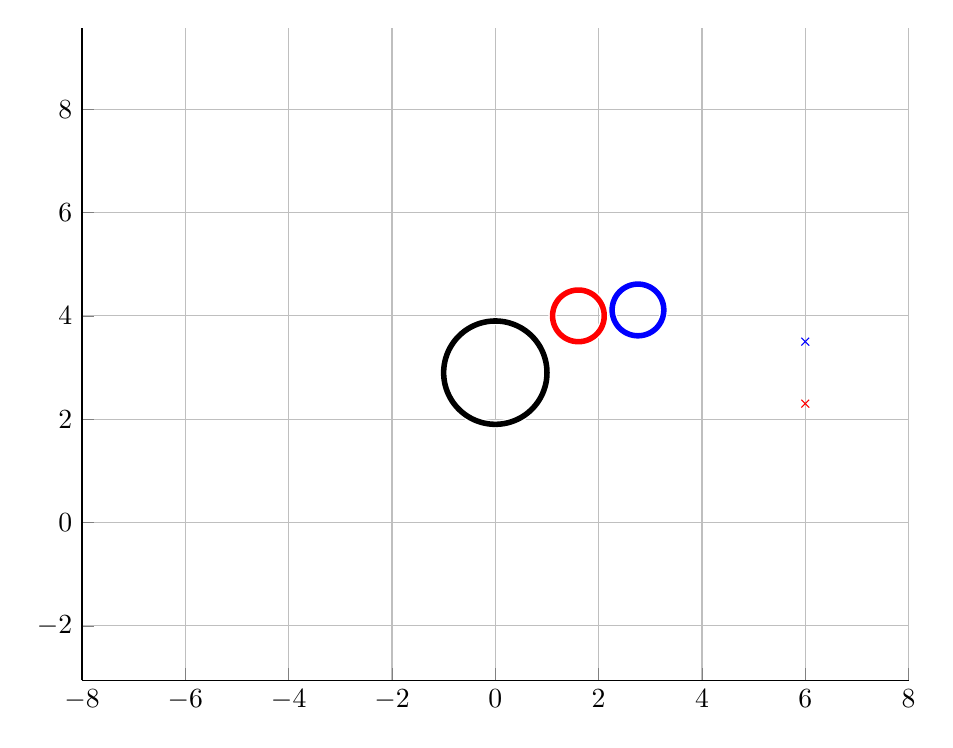
\begin{tikzpicture}

\begin{axis}[%
width=4.133in,
height=3.26in,
at={(0.693in,0.44in)},
scale only axis,
unbounded coords=jump,
xmin=-8,
xmax=8,
xmajorgrids,
ymin=-3.05283025828205,
ymax=9.56652458042763,
ymajorgrids,
axis background/.style={fill=white},
axis x line*=bottom,
axis y line*=left
]
\addplot [color=blue,only marks,mark=x,mark options={solid},forget plot]
  table[row sep=crcr]{%
6	3.5\\
};
\addplot [color=red,only marks,mark=x,mark options={solid},forget plot]
  table[row sep=crcr]{%
6	2.3\\
};
\addplot [color=white,solid,line width=3.0pt,forget plot]
  table[row sep=crcr]{%
3.26105064544558	4.11369432214559\\
3.26074605895513	4.13114407049684\\
3.25983267057549	4.14857255901765\\
3.25831159312971	4.16595855377941\\
3.25618467981636	4.18328087262562\\
3.25345452195168	4.20051841097905\\
3.25012444581248	4.21765016755447\\
3.24619850858358	4.23465526994542\\
3.24168149341474	4.25151300005408\\
3.23657890359315	4.26820281933306\\
3.23089695583853	4.28470439380842\\
3.22464257272897	4.30099761885354\\
3.21782337426688	4.31706264368349\\
3.21044766859516	4.33287989554012\\
3.20252444187504	4.34843010353853\\
3.1940633473378	4.36369432214559\\
3.18507469352379	4.37865395426219\\
3.1755694317231	4.39329077388096\\
3.16555914263305	4.40758694829182\\
3.15505602224894	4.42152505980842\\
3.14407286700507	4.43508812698886\\
3.13262305818427	4.44825962532502\\
3.1207205456149	4.46102350737508\\
3.10837983067508	4.47336422231491\\
3.09561594862501	4.48526673488428\\
3.08244445028885	4.49671654370507\\
3.06888138310841	4.50769969894895\\
3.05494327159181	4.51820281933306\\
3.04064709718095	4.52821310842311\\
3.02601027756218	4.5377183702238\\
3.01105064544558	4.54670702403781\\
2.99578642683852	4.55516811857505\\
2.98023621884012	4.56309134529517\\
2.96441896698348	4.57046705096689\\
2.94835394215353	4.57728624942898\\
2.93206071710841	4.58354063253854\\
2.91555914263305	4.58922258029316\\
2.89886932335408	4.59432517011474\\
2.88201159324541	4.59884218528358\\
2.86500649085446	4.60276812251249\\
2.84787473427904	4.60609819865169\\
2.83063719592561	4.60882835651637\\
2.8133148770794	4.61095526982972\\
2.79592888231764	4.6124763472755\\
2.77850039379683	4.61338973565513\\
2.76105064544558	4.61369432214559\\
2.74360089709433	4.61338973565513\\
2.72617240857352	4.6124763472755\\
2.70878641381175	4.61095526982972\\
2.69146409496555	4.60882835651637\\
2.67422655661211	4.60609819865169\\
2.6570948000367	4.60276812251249\\
2.64008969764574	4.59884218528358\\
2.62323196753708	4.59432517011474\\
2.6065421482581	4.58922258029316\\
2.59004057378274	4.58354063253854\\
2.57374734873762	4.57728624942898\\
2.55768232390768	4.57046705096689\\
2.54186507205104	4.56309134529517\\
2.52631486405263	4.55516811857505\\
2.51105064544558	4.54670702403781\\
2.49609101332898	4.5377183702238\\
2.4814541937102	4.52821310842311\\
2.46715801929934	4.51820281933306\\
2.45321990778275	4.50769969894895\\
2.43965684060231	4.49671654370507\\
2.42648534226615	4.48526673488428\\
2.41372146021608	4.47336422231491\\
2.40138074527625	4.46102350737508\\
2.38947823270688	4.44825962532502\\
2.37802842388609	4.43508812698886\\
2.36704526864222	4.42152505980842\\
2.3565421482581	4.40758694829182\\
2.34653185916806	4.39329077388096\\
2.33702659736736	4.37865395426219\\
2.32803794355336	4.36369432214559\\
2.31957684901611	4.34843010353853\\
2.31165362229599	4.33287989554012\\
2.30427791662428	4.31706264368349\\
2.29745871816218	4.30099761885354\\
2.29120433505262	4.28470439380842\\
2.285522387298	4.26820281933306\\
2.28041979747642	4.25151300005409\\
2.27590278230758	4.23465526994542\\
2.27197684507868	4.21765016755447\\
2.26864676893947	4.20051841097905\\
2.26591661107479	4.18328087262562\\
2.26378969776144	4.16595855377941\\
2.26226862031567	4.14857255901765\\
2.26135523193603	4.13114407049684\\
2.26105064544558	4.11369432214559\\
2.26135523193603	4.09624457379434\\
2.26226862031567	4.07881608527352\\
2.26378969776144	4.06143009051176\\
2.26591661107479	4.04410777166555\\
2.26864676893947	4.02687023331212\\
2.27197684507868	4.00973847673671\\
2.27590278230758	3.99273337434575\\
2.28041979747642	3.97587564423709\\
2.285522387298	3.95918582495811\\
2.29120433505262	3.94268425048275\\
2.29745871816218	3.92639102543763\\
2.30427791662428	3.91032600060769\\
2.31165362229599	3.89450874875105\\
2.31957684901611	3.87895854075264\\
2.32803794355336	3.86369432214559\\
2.33702659736736	3.84873469002898\\
2.34653185916806	3.83409787041021\\
2.3565421482581	3.81980169599935\\
2.36704526864222	3.80586358448276\\
2.37802842388609	3.79230051730232\\
2.38947823270688	3.77912901896616\\
2.40138074527625	3.76636513691609\\
2.41372146021608	3.75402442197626\\
2.42648534226615	3.74212190940689\\
2.43965684060231	3.7306721005861\\
2.45321990778275	3.71968894534222\\
2.46715801929934	3.70918582495811\\
2.4814541937102	3.69917553586806\\
2.49609101332898	3.68967027406737\\
2.51105064544558	3.68068162025337\\
2.52631486405263	3.67222052571612\\
2.54186507205104	3.664297298996\\
2.55768232390768	3.65692159332428\\
2.57374734873762	3.65010239486219\\
2.59004057378274	3.64384801175263\\
2.6065421482581	3.63816606399801\\
2.62323196753708	3.63306347417643\\
2.64008969764574	3.62854645900759\\
2.6570948000367	3.62462052177868\\
2.67422655661211	3.62129044563948\\
2.69146409496555	3.6185602877748\\
2.70878641381175	3.61643337446145\\
2.72617240857352	3.61491229701567\\
2.74360089709433	3.61399890863604\\
2.76105064544558	3.61369432214559\\
2.77850039379683	3.61399890863604\\
2.79592888231764	3.61491229701567\\
2.8133148770794	3.61643337446145\\
2.83063719592561	3.6185602877748\\
2.84787473427904	3.62129044563948\\
2.86500649085446	3.62462052177868\\
2.88201159324541	3.62854645900759\\
2.89886932335408	3.63306347417643\\
2.91555914263305	3.63816606399801\\
2.93206071710841	3.64384801175263\\
2.94835394215353	3.65010239486219\\
2.96441896698348	3.65692159332429\\
2.98023621884012	3.664297298996\\
2.99578642683852	3.67222052571612\\
3.01105064544558	3.68068162025337\\
3.02601027756218	3.68967027406737\\
3.04064709718095	3.69917553586806\\
3.05494327159181	3.70918582495811\\
3.06888138310841	3.71968894534222\\
3.08244445028885	3.7306721005861\\
3.09561594862501	3.74212190940689\\
3.10837983067508	3.75402442197626\\
3.1207205456149	3.76636513691609\\
3.13262305818427	3.77912901896616\\
3.14407286700507	3.79230051730232\\
3.15505602224894	3.80586358448276\\
3.16555914263305	3.81980169599935\\
3.1755694317231	3.83409787041021\\
3.18507469352379	3.84873469002898\\
3.1940633473378	3.86369432214559\\
3.20252444187504	3.87895854075264\\
3.21044766859516	3.89450874875105\\
3.21782337426688	3.91032600060769\\
3.22464257272897	3.92639102543763\\
3.23089695583853	3.94268425048275\\
3.23657890359315	3.95918582495811\\
3.24168149341474	3.97587564423709\\
3.24619850858358	3.99273337434575\\
3.25012444581248	4.00973847673671\\
3.25345452195168	4.02687023331212\\
3.25618467981636	4.04410777166555\\
3.25831159312971	4.06143009051176\\
3.25983267057549	4.07881608527352\\
3.26074605895513	4.09624457379434\\
3.26105064544558	4.11369432214559\\
nan	nan\\
};
\addplot [color=blue,solid,line width=2.0pt,forget plot]
  table[row sep=crcr]{%
3.26105064544558	4.11369432214559\\
3.26074605895513	4.13114407049684\\
3.25983267057549	4.14857255901765\\
3.25831159312971	4.16595855377941\\
3.25618467981636	4.18328087262562\\
3.25345452195168	4.20051841097905\\
3.25012444581248	4.21765016755447\\
3.24619850858358	4.23465526994542\\
3.24168149341474	4.25151300005408\\
3.23657890359315	4.26820281933306\\
3.23089695583853	4.28470439380842\\
3.22464257272897	4.30099761885354\\
3.21782337426688	4.31706264368349\\
3.21044766859516	4.33287989554012\\
3.20252444187504	4.34843010353853\\
3.1940633473378	4.36369432214559\\
3.18507469352379	4.37865395426219\\
3.1755694317231	4.39329077388096\\
3.16555914263305	4.40758694829182\\
3.15505602224894	4.42152505980842\\
3.14407286700507	4.43508812698886\\
3.13262305818427	4.44825962532502\\
3.1207205456149	4.46102350737508\\
3.10837983067508	4.47336422231491\\
3.09561594862501	4.48526673488428\\
3.08244445028885	4.49671654370507\\
3.06888138310841	4.50769969894895\\
3.05494327159181	4.51820281933306\\
3.04064709718095	4.52821310842311\\
3.02601027756218	4.5377183702238\\
3.01105064544558	4.54670702403781\\
2.99578642683852	4.55516811857505\\
2.98023621884012	4.56309134529517\\
2.96441896698348	4.57046705096689\\
2.94835394215353	4.57728624942898\\
2.93206071710841	4.58354063253854\\
2.91555914263305	4.58922258029316\\
2.89886932335408	4.59432517011474\\
2.88201159324541	4.59884218528358\\
2.86500649085446	4.60276812251249\\
2.84787473427904	4.60609819865169\\
2.83063719592561	4.60882835651637\\
2.8133148770794	4.61095526982972\\
2.79592888231764	4.6124763472755\\
2.77850039379683	4.61338973565513\\
2.76105064544558	4.61369432214559\\
2.74360089709433	4.61338973565513\\
2.72617240857352	4.6124763472755\\
2.70878641381175	4.61095526982972\\
2.69146409496555	4.60882835651637\\
2.67422655661211	4.60609819865169\\
2.6570948000367	4.60276812251249\\
2.64008969764574	4.59884218528358\\
2.62323196753708	4.59432517011474\\
2.6065421482581	4.58922258029316\\
2.59004057378274	4.58354063253854\\
2.57374734873762	4.57728624942898\\
2.55768232390768	4.57046705096689\\
2.54186507205104	4.56309134529517\\
2.52631486405263	4.55516811857505\\
2.51105064544558	4.54670702403781\\
2.49609101332898	4.5377183702238\\
2.4814541937102	4.52821310842311\\
2.46715801929934	4.51820281933306\\
2.45321990778275	4.50769969894895\\
2.43965684060231	4.49671654370507\\
2.42648534226615	4.48526673488428\\
2.41372146021608	4.47336422231491\\
2.40138074527625	4.46102350737508\\
2.38947823270688	4.44825962532502\\
2.37802842388609	4.43508812698886\\
2.36704526864222	4.42152505980842\\
2.3565421482581	4.40758694829182\\
2.34653185916806	4.39329077388096\\
2.33702659736736	4.37865395426219\\
2.32803794355336	4.36369432214559\\
2.31957684901611	4.34843010353853\\
2.31165362229599	4.33287989554012\\
2.30427791662428	4.31706264368349\\
2.29745871816218	4.30099761885354\\
2.29120433505262	4.28470439380842\\
2.285522387298	4.26820281933306\\
2.28041979747642	4.25151300005409\\
2.27590278230758	4.23465526994542\\
2.27197684507868	4.21765016755447\\
2.26864676893947	4.20051841097905\\
2.26591661107479	4.18328087262562\\
2.26378969776144	4.16595855377941\\
2.26226862031567	4.14857255901765\\
2.26135523193603	4.13114407049684\\
2.26105064544558	4.11369432214559\\
2.26135523193603	4.09624457379434\\
2.26226862031567	4.07881608527352\\
2.26378969776144	4.06143009051176\\
2.26591661107479	4.04410777166555\\
2.26864676893947	4.02687023331212\\
2.27197684507868	4.00973847673671\\
2.27590278230758	3.99273337434575\\
2.28041979747642	3.97587564423709\\
2.285522387298	3.95918582495811\\
2.29120433505262	3.94268425048275\\
2.29745871816218	3.92639102543763\\
2.30427791662428	3.91032600060769\\
2.31165362229599	3.89450874875105\\
2.31957684901611	3.87895854075264\\
2.32803794355336	3.86369432214559\\
2.33702659736736	3.84873469002898\\
2.34653185916806	3.83409787041021\\
2.3565421482581	3.81980169599935\\
2.36704526864222	3.80586358448276\\
2.37802842388609	3.79230051730232\\
2.38947823270688	3.77912901896616\\
2.40138074527625	3.76636513691609\\
2.41372146021608	3.75402442197626\\
2.42648534226615	3.74212190940689\\
2.43965684060231	3.7306721005861\\
2.45321990778275	3.71968894534222\\
2.46715801929934	3.70918582495811\\
2.4814541937102	3.69917553586806\\
2.49609101332898	3.68967027406737\\
2.51105064544558	3.68068162025337\\
2.52631486405263	3.67222052571612\\
2.54186507205104	3.664297298996\\
2.55768232390768	3.65692159332428\\
2.57374734873762	3.65010239486219\\
2.59004057378274	3.64384801175263\\
2.6065421482581	3.63816606399801\\
2.62323196753708	3.63306347417643\\
2.64008969764574	3.62854645900759\\
2.6570948000367	3.62462052177868\\
2.67422655661211	3.62129044563948\\
2.69146409496555	3.6185602877748\\
2.70878641381175	3.61643337446145\\
2.72617240857352	3.61491229701567\\
2.74360089709433	3.61399890863604\\
2.76105064544558	3.61369432214559\\
2.77850039379683	3.61399890863604\\
2.79592888231764	3.61491229701567\\
2.8133148770794	3.61643337446145\\
2.83063719592561	3.6185602877748\\
2.84787473427904	3.62129044563948\\
2.86500649085446	3.62462052177868\\
2.88201159324541	3.62854645900759\\
2.89886932335408	3.63306347417643\\
2.91555914263305	3.63816606399801\\
2.93206071710841	3.64384801175263\\
2.94835394215353	3.65010239486219\\
2.96441896698348	3.65692159332429\\
2.98023621884012	3.664297298996\\
2.99578642683852	3.67222052571612\\
3.01105064544558	3.68068162025337\\
3.02601027756218	3.68967027406737\\
3.04064709718095	3.69917553586806\\
3.05494327159181	3.70918582495811\\
3.06888138310841	3.71968894534222\\
3.08244445028885	3.7306721005861\\
3.09561594862501	3.74212190940689\\
3.10837983067508	3.75402442197626\\
3.1207205456149	3.76636513691609\\
3.13262305818427	3.77912901896616\\
3.14407286700507	3.79230051730232\\
3.15505602224894	3.80586358448276\\
3.16555914263305	3.81980169599935\\
3.1755694317231	3.83409787041021\\
3.18507469352379	3.84873469002898\\
3.1940633473378	3.86369432214559\\
3.20252444187504	3.87895854075264\\
3.21044766859516	3.89450874875105\\
3.21782337426688	3.91032600060769\\
3.22464257272897	3.92639102543763\\
3.23089695583853	3.94268425048275\\
3.23657890359315	3.95918582495811\\
3.24168149341474	3.97587564423709\\
3.24619850858358	3.99273337434575\\
3.25012444581248	4.00973847673671\\
3.25345452195168	4.02687023331212\\
3.25618467981636	4.04410777166555\\
3.25831159312971	4.06143009051176\\
3.25983267057549	4.07881608527352\\
3.26074605895513	4.09624457379434\\
3.26105064544558	4.11369432214559\\
nan	nan\\
};
\addplot [color=white,solid,line width=3.0pt,forget plot]
  table[row sep=crcr]{%
2.10804355233902	3.99928625125649\\
2.10773896584857	4.01673599960774\\
2.10682557746893	4.03416448812856\\
2.10530450002316	4.05155048289032\\
2.1031775867098	4.06887280173653\\
2.10044742884512	4.08611034008996\\
2.09711735270592	4.10324209666537\\
2.09319141547702	4.12024719905633\\
2.08867440030818	4.13710492916499\\
2.0835718104866	4.15379474844397\\
2.07788986273197	4.17029632291933\\
2.07163547962241	4.18658954796445\\
2.06481628116032	4.20265457279439\\
2.0574405754886	4.21847182465103\\
2.04951734876848	4.23402203264944\\
2.04105625423124	4.24928625125649\\
2.03206760041723	4.2642458833731\\
2.02256233861654	4.27888270299187\\
2.01255204952649	4.29317887740273\\
2.00204892914238	4.30711698891932\\
1.99106577389851	4.32068005609976\\
1.97961596507772	4.33385155443592\\
1.96771345250834	4.34661543648599\\
1.95537273756852	4.35895615142582\\
1.94260885551845	4.37085866399519\\
1.92943735718229	4.38230847281598\\
1.91587429000185	4.39329162805985\\
1.90193617848526	4.40379474844397\\
1.88764000407439	4.41380503753401\\
1.87300318445562	4.42331029933471\\
1.85804355233902	4.43229895314871\\
1.84277933373196	4.44076004768596\\
1.82722912573356	4.44868327440608\\
1.81141187387692	4.45605898007779\\
1.79534684904697	4.46287817853989\\
1.77905362400185	4.46913256164945\\
1.76255204952649	4.47481450940407\\
1.74586223024752	4.47991709922565\\
1.72900450013885	4.48443411439449\\
1.7119993977479	4.4883600516234\\
1.69486764117248	4.4916901277626\\
1.67763010281905	4.49442028562728\\
1.66030778397285	4.49654719894063\\
1.64292178921108	4.49806827638641\\
1.62549330069027	4.49898166476604\\
1.60804355233902	4.49928625125649\\
1.59059380398777	4.49898166476604\\
1.57316531546696	4.49806827638641\\
1.55577932070519	4.49654719894063\\
1.53845700185899	4.49442028562728\\
1.52121946350555	4.4916901277626\\
1.50408770693014	4.4883600516234\\
1.48708260453918	4.48443411439449\\
1.47022487443052	4.47991709922565\\
1.45353505515154	4.47481450940407\\
1.43703348067618	4.46913256164945\\
1.42074025563106	4.46287817853989\\
1.40467523080112	4.45605898007779\\
1.38885797894448	4.44868327440608\\
1.37330777094607	4.44076004768596\\
1.35804355233902	4.43229895314871\\
1.34308392022242	4.42331029933471\\
1.32844710060365	4.41380503753401\\
1.31415092619278	4.40379474844397\\
1.30021281467619	4.39329162805985\\
1.28664974749575	4.38230847281598\\
1.27347824915959	4.37085866399519\\
1.26071436710952	4.35895615142582\\
1.24837365216969	4.34661543648599\\
1.23647113960032	4.33385155443592\\
1.22502133077953	4.32068005609976\\
1.21403817553566	4.30711698891932\\
1.20353505515154	4.29317887740273\\
1.1935247660615	4.27888270299187\\
1.18401950426081	4.2642458833731\\
1.1750308504468	4.24928625125649\\
1.16656975590955	4.23402203264944\\
1.15864652918944	4.21847182465103\\
1.15127082351772	4.20265457279439\\
1.14445162505562	4.18658954796445\\
1.13819724194606	4.17029632291933\\
1.13251529419144	4.15379474844397\\
1.12741270436986	4.13710492916499\\
1.12289568920102	4.12024719905633\\
1.11896975197212	4.10324209666537\\
1.11563967583291	4.08611034008996\\
1.11290951796823	4.06887280173653\\
1.11078260465488	4.05155048289032\\
1.10926152720911	4.03416448812856\\
1.10834813882947	4.01673599960774\\
1.10804355233902	3.99928625125649\\
1.10834813882947	3.98183650290524\\
1.10926152720911	3.96440801438443\\
1.11078260465488	3.94702201962267\\
1.11290951796823	3.92969970077646\\
1.11563967583291	3.91246216242303\\
1.11896975197212	3.89533040584761\\
1.12289568920102	3.87832530345666\\
1.12741270436986	3.86146757334799\\
1.13251529419144	3.84477775406902\\
1.13819724194606	3.82827617959366\\
1.14445162505562	3.81198295454854\\
1.15127082351772	3.79591792971859\\
1.15864652918943	3.78010067786195\\
1.16656975590955	3.76455046986355\\
1.1750308504468	3.74928625125649\\
1.18401950426081	3.73432661913989\\
1.1935247660615	3.71968979952112\\
1.20353505515154	3.70539362511026\\
1.21403817553566	3.69145551359366\\
1.22502133077953	3.67789244641322\\
1.23647113960032	3.66472094807706\\
1.24837365216969	3.65195706602699\\
1.26071436710952	3.63961635108717\\
1.27347824915959	3.6277138385178\\
1.28664974749575	3.616264029697\\
1.30021281467619	3.60528087445313\\
1.31415092619278	3.59477775406902\\
1.32844710060364	3.58476746497897\\
1.34308392022242	3.57526220317828\\
1.35804355233902	3.56627354936427\\
1.37330777094607	3.55781245482703\\
1.38885797894448	3.54988922810691\\
1.40467523080112	3.54251352243519\\
1.42074025563106	3.5356943239731\\
1.43703348067618	3.52943994086354\\
1.45353505515154	3.52375799310892\\
1.47022487443052	3.51865540328733\\
1.48708260453918	3.51413838811849\\
1.50408770693014	3.51021245088959\\
1.52121946350555	3.50688237475039\\
1.53845700185899	3.50415221688571\\
1.55577932070519	3.50202530357236\\
1.57316531546696	3.50050422612658\\
1.59059380398777	3.49959083774695\\
1.60804355233902	3.49928625125649\\
1.62549330069027	3.49959083774695\\
1.64292178921108	3.50050422612658\\
1.66030778397284	3.50202530357236\\
1.67763010281905	3.50415221688571\\
1.69486764117248	3.50688237475039\\
1.7119993977479	3.51021245088959\\
1.72900450013885	3.51413838811849\\
1.74586223024752	3.51865540328733\\
1.76255204952649	3.52375799310892\\
1.77905362400185	3.52943994086354\\
1.79534684904697	3.5356943239731\\
1.81141187387692	3.54251352243519\\
1.82722912573356	3.54988922810691\\
1.84277933373196	3.55781245482703\\
1.85804355233902	3.56627354936427\\
1.87300318445562	3.57526220317828\\
1.88764000407439	3.58476746497897\\
1.90193617848525	3.59477775406902\\
1.91587429000185	3.60528087445313\\
1.92943735718229	3.616264029697\\
1.94260885551845	3.6277138385178\\
1.95537273756852	3.63961635108717\\
1.96771345250834	3.65195706602699\\
1.97961596507772	3.66472094807706\\
1.99106577389851	3.67789244641322\\
2.00204892914238	3.69145551359366\\
2.01255204952649	3.70539362511026\\
2.02256233861654	3.71968979952112\\
2.03206760041723	3.73432661913989\\
2.04105625423124	3.74928625125649\\
2.04951734876848	3.76455046986355\\
2.0574405754886	3.78010067786195\\
2.06481628116032	3.79591792971859\\
2.07163547962241	3.81198295454854\\
2.07788986273197	3.82827617959366\\
2.0835718104866	3.84477775406902\\
2.08867440030818	3.86146757334799\\
2.09319141547702	3.87832530345666\\
2.09711735270592	3.89533040584761\\
2.10044742884512	3.91246216242303\\
2.1031775867098	3.92969970077646\\
2.10530450002316	3.94702201962267\\
2.10682557746893	3.96440801438443\\
2.10773896584857	3.98183650290524\\
2.10804355233902	3.99928625125649\\
nan	nan\\
};
\addplot [color=red,solid,line width=2.0pt,forget plot]
  table[row sep=crcr]{%
2.10804355233902	3.99928625125649\\
2.10773896584857	4.01673599960774\\
2.10682557746893	4.03416448812856\\
2.10530450002316	4.05155048289032\\
2.1031775867098	4.06887280173653\\
2.10044742884512	4.08611034008996\\
2.09711735270592	4.10324209666537\\
2.09319141547702	4.12024719905633\\
2.08867440030818	4.13710492916499\\
2.0835718104866	4.15379474844397\\
2.07788986273197	4.17029632291933\\
2.07163547962241	4.18658954796445\\
2.06481628116032	4.20265457279439\\
2.0574405754886	4.21847182465103\\
2.04951734876848	4.23402203264944\\
2.04105625423124	4.24928625125649\\
2.03206760041723	4.2642458833731\\
2.02256233861654	4.27888270299187\\
2.01255204952649	4.29317887740273\\
2.00204892914238	4.30711698891932\\
1.99106577389851	4.32068005609976\\
1.97961596507772	4.33385155443592\\
1.96771345250834	4.34661543648599\\
1.95537273756852	4.35895615142582\\
1.94260885551845	4.37085866399519\\
1.92943735718229	4.38230847281598\\
1.91587429000185	4.39329162805985\\
1.90193617848526	4.40379474844397\\
1.88764000407439	4.41380503753401\\
1.87300318445562	4.42331029933471\\
1.85804355233902	4.43229895314871\\
1.84277933373196	4.44076004768596\\
1.82722912573356	4.44868327440608\\
1.81141187387692	4.45605898007779\\
1.79534684904697	4.46287817853989\\
1.77905362400185	4.46913256164945\\
1.76255204952649	4.47481450940407\\
1.74586223024752	4.47991709922565\\
1.72900450013885	4.48443411439449\\
1.7119993977479	4.4883600516234\\
1.69486764117248	4.4916901277626\\
1.67763010281905	4.49442028562728\\
1.66030778397285	4.49654719894063\\
1.64292178921108	4.49806827638641\\
1.62549330069027	4.49898166476604\\
1.60804355233902	4.49928625125649\\
1.59059380398777	4.49898166476604\\
1.57316531546696	4.49806827638641\\
1.55577932070519	4.49654719894063\\
1.53845700185899	4.49442028562728\\
1.52121946350555	4.4916901277626\\
1.50408770693014	4.4883600516234\\
1.48708260453918	4.48443411439449\\
1.47022487443052	4.47991709922565\\
1.45353505515154	4.47481450940407\\
1.43703348067618	4.46913256164945\\
1.42074025563106	4.46287817853989\\
1.40467523080112	4.45605898007779\\
1.38885797894448	4.44868327440608\\
1.37330777094607	4.44076004768596\\
1.35804355233902	4.43229895314871\\
1.34308392022242	4.42331029933471\\
1.32844710060365	4.41380503753401\\
1.31415092619278	4.40379474844397\\
1.30021281467619	4.39329162805985\\
1.28664974749575	4.38230847281598\\
1.27347824915959	4.37085866399519\\
1.26071436710952	4.35895615142582\\
1.24837365216969	4.34661543648599\\
1.23647113960032	4.33385155443592\\
1.22502133077953	4.32068005609976\\
1.21403817553566	4.30711698891932\\
1.20353505515154	4.29317887740273\\
1.1935247660615	4.27888270299187\\
1.18401950426081	4.2642458833731\\
1.1750308504468	4.24928625125649\\
1.16656975590955	4.23402203264944\\
1.15864652918944	4.21847182465103\\
1.15127082351772	4.20265457279439\\
1.14445162505562	4.18658954796445\\
1.13819724194606	4.17029632291933\\
1.13251529419144	4.15379474844397\\
1.12741270436986	4.13710492916499\\
1.12289568920102	4.12024719905633\\
1.11896975197212	4.10324209666537\\
1.11563967583291	4.08611034008996\\
1.11290951796823	4.06887280173653\\
1.11078260465488	4.05155048289032\\
1.10926152720911	4.03416448812856\\
1.10834813882947	4.01673599960774\\
1.10804355233902	3.99928625125649\\
1.10834813882947	3.98183650290524\\
1.10926152720911	3.96440801438443\\
1.11078260465488	3.94702201962267\\
1.11290951796823	3.92969970077646\\
1.11563967583291	3.91246216242303\\
1.11896975197212	3.89533040584761\\
1.12289568920102	3.87832530345666\\
1.12741270436986	3.86146757334799\\
1.13251529419144	3.84477775406902\\
1.13819724194606	3.82827617959366\\
1.14445162505562	3.81198295454854\\
1.15127082351772	3.79591792971859\\
1.15864652918943	3.78010067786195\\
1.16656975590955	3.76455046986355\\
1.1750308504468	3.74928625125649\\
1.18401950426081	3.73432661913989\\
1.1935247660615	3.71968979952112\\
1.20353505515154	3.70539362511026\\
1.21403817553566	3.69145551359366\\
1.22502133077953	3.67789244641322\\
1.23647113960032	3.66472094807706\\
1.24837365216969	3.65195706602699\\
1.26071436710952	3.63961635108717\\
1.27347824915959	3.6277138385178\\
1.28664974749575	3.616264029697\\
1.30021281467619	3.60528087445313\\
1.31415092619278	3.59477775406902\\
1.32844710060364	3.58476746497897\\
1.34308392022242	3.57526220317828\\
1.35804355233902	3.56627354936427\\
1.37330777094607	3.55781245482703\\
1.38885797894448	3.54988922810691\\
1.40467523080112	3.54251352243519\\
1.42074025563106	3.5356943239731\\
1.43703348067618	3.52943994086354\\
1.45353505515154	3.52375799310892\\
1.47022487443052	3.51865540328733\\
1.48708260453918	3.51413838811849\\
1.50408770693014	3.51021245088959\\
1.52121946350555	3.50688237475039\\
1.53845700185899	3.50415221688571\\
1.55577932070519	3.50202530357236\\
1.57316531546696	3.50050422612658\\
1.59059380398777	3.49959083774695\\
1.60804355233902	3.49928625125649\\
1.62549330069027	3.49959083774695\\
1.64292178921108	3.50050422612658\\
1.66030778397284	3.50202530357236\\
1.67763010281905	3.50415221688571\\
1.69486764117248	3.50688237475039\\
1.7119993977479	3.51021245088959\\
1.72900450013885	3.51413838811849\\
1.74586223024752	3.51865540328733\\
1.76255204952649	3.52375799310892\\
1.77905362400185	3.52943994086354\\
1.79534684904697	3.5356943239731\\
1.81141187387692	3.54251352243519\\
1.82722912573356	3.54988922810691\\
1.84277933373196	3.55781245482703\\
1.85804355233902	3.56627354936427\\
1.87300318445562	3.57526220317828\\
1.88764000407439	3.58476746497897\\
1.90193617848525	3.59477775406902\\
1.91587429000185	3.60528087445313\\
1.92943735718229	3.616264029697\\
1.94260885551845	3.6277138385178\\
1.95537273756852	3.63961635108717\\
1.96771345250834	3.65195706602699\\
1.97961596507772	3.66472094807706\\
1.99106577389851	3.67789244641322\\
2.00204892914238	3.69145551359366\\
2.01255204952649	3.70539362511026\\
2.02256233861654	3.71968979952112\\
2.03206760041723	3.73432661913989\\
2.04105625423124	3.74928625125649\\
2.04951734876848	3.76455046986355\\
2.0574405754886	3.78010067786195\\
2.06481628116032	3.79591792971859\\
2.07163547962241	3.81198295454854\\
2.07788986273197	3.82827617959366\\
2.0835718104866	3.84477775406902\\
2.08867440030818	3.86146757334799\\
2.09319141547702	3.87832530345666\\
2.09711735270592	3.89533040584761\\
2.10044742884512	3.91246216242303\\
2.1031775867098	3.92969970077646\\
2.10530450002316	3.94702201962267\\
2.10682557746893	3.96440801438443\\
2.10773896584857	3.98183650290524\\
2.10804355233902	3.99928625125649\\
nan	nan\\
};
\addplot [color=white,solid,line width=3.0pt,forget plot]
  table[row sep=crcr]{%
1	2.9\\
0.999390827019096	2.9348994967025\\
0.997564050259824	2.96975647374413\\
0.994521895368273	3.00452846326765\\
0.99026806874157	3.03917310096007\\
0.984807753012208	3.07364817766693\\
0.978147600733806	3.10791169081776\\
0.970295726275996	3.14192189559967\\
0.961261695938319	3.175637355817\\
0.951056516295154	3.20901699437495\\
0.939692620785908	3.24202014332567\\
0.927183854566787	3.27460659341591\\
0.913545457642601	3.3067366430758\\
0.898794046299167	3.33837114678908\\
0.882947592858927	3.36947156278589\\
0.866025403784439	3.4\\
0.848048096156426	3.42991926423321\\
0.829037572555042	3.45919290347075\\
0.809016994374947	3.48778525229247\\
0.788010753606722	3.51566147532566\\
0.766044443118978	3.54278760968654\\
0.743144825477394	3.56913060635886\\
0.719339800338651	3.594658370459\\
0.694658370458997	3.61933980033865\\
0.669130606358858	3.64314482547739\\
0.642787609686539	3.66604444311898\\
0.615661475325658	3.68801075360672\\
0.587785252292473	3.70901699437495\\
0.559192903470747	3.72903757255504\\
0.529919264233205	3.74804809615643\\
0.5	3.76602540378444\\
0.469471562785891	3.78294759285893\\
0.438371146789077	3.79879404629917\\
0.4067366430758	3.8135454576426\\
0.374606593415912	3.82718385456679\\
0.342020143325669	3.83969262078591\\
0.309016994374947	3.85105651629515\\
0.275637355816999	3.86126169593832\\
0.241921895599668	3.870295726276\\
0.207911690817759	3.87814760073381\\
0.17364817766693	3.88480775301221\\
0.139173100960066	3.89026806874157\\
0.104528463267653	3.89452189536827\\
0.0697564737441255	3.89756405025982\\
0.0348994967025011	3.8993908270191\\
6.12323399573677e-17	3.9\\
-0.0348994967025007	3.8993908270191\\
-0.0697564737441253	3.89756405025982\\
-0.104528463267653	3.89452189536827\\
-0.139173100960065	3.89026806874157\\
-0.17364817766693	3.88480775301221\\
-0.207911690817759	3.87814760073381\\
-0.241921895599668	3.870295726276\\
-0.275637355816999	3.86126169593832\\
-0.309016994374947	3.85105651629515\\
-0.342020143325669	3.83969262078591\\
-0.374606593415912	3.82718385456679\\
-0.4067366430758	3.8135454576426\\
-0.438371146789078	3.79879404629917\\
-0.469471562785891	3.78294759285893\\
-0.5	3.76602540378444\\
-0.529919264233205	3.74804809615643\\
-0.559192903470747	3.72903757255504\\
-0.587785252292473	3.70901699437495\\
-0.615661475325658	3.68801075360672\\
-0.642787609686539	3.66604444311898\\
-0.669130606358858	3.64314482547739\\
-0.694658370458997	3.61933980033865\\
-0.719339800338651	3.594658370459\\
-0.743144825477394	3.56913060635886\\
-0.766044443118978	3.54278760968654\\
-0.788010753606722	3.51566147532566\\
-0.809016994374947	3.48778525229247\\
-0.829037572555042	3.45919290347075\\
-0.848048096156426	3.42991926423321\\
-0.866025403784439	3.4\\
-0.882947592858927	3.36947156278589\\
-0.898794046299167	3.33837114678908\\
-0.913545457642601	3.3067366430758\\
-0.927183854566787	3.27460659341591\\
-0.939692620785908	3.24202014332567\\
-0.951056516295154	3.20901699437495\\
-0.961261695938319	3.175637355817\\
-0.970295726275996	3.14192189559967\\
-0.978147600733806	3.10791169081776\\
-0.984807753012208	3.07364817766693\\
-0.99026806874157	3.03917310096007\\
-0.994521895368273	3.00452846326765\\
-0.997564050259824	2.96975647374413\\
-0.999390827019096	2.9348994967025\\
-1	2.9\\
-0.999390827019096	2.8651005032975\\
-0.997564050259824	2.83024352625588\\
-0.994521895368273	2.79547153673235\\
-0.99026806874157	2.76082689903993\\
-0.984807753012208	2.72635182233307\\
-0.978147600733806	2.69208830918224\\
-0.970295726275997	2.65807810440033\\
-0.961261695938319	2.624362644183\\
-0.951056516295154	2.59098300562505\\
-0.939692620785908	2.55797985667433\\
-0.927183854566787	2.52539340658409\\
-0.913545457642601	2.4932633569242\\
-0.898794046299167	2.46162885321092\\
-0.882947592858927	2.43052843721411\\
-0.866025403784439	2.4\\
-0.848048096156426	2.3700807357668\\
-0.829037572555042	2.34080709652925\\
-0.809016994374947	2.31221474770753\\
-0.788010753606722	2.28433852467434\\
-0.766044443118978	2.25721239031346\\
-0.743144825477394	2.23086939364114\\
-0.719339800338651	2.205341629541\\
-0.694658370458997	2.18066019966135\\
-0.669130606358858	2.15685517452261\\
-0.642787609686539	2.13395555688102\\
-0.615661475325658	2.11198924639328\\
-0.587785252292473	2.09098300562505\\
-0.559192903470747	2.07096242744496\\
-0.529919264233205	2.05195190384357\\
-0.5	2.03397459621556\\
-0.469471562785891	2.01705240714107\\
-0.438371146789078	2.00120595370083\\
-0.4067366430758	1.9864545423574\\
-0.374606593415912	1.97281614543321\\
-0.342020143325669	1.96030737921409\\
-0.309016994374948	1.94894348370485\\
-0.275637355816999	1.93873830406168\\
-0.241921895599668	1.929704273724\\
-0.20791169081776	1.92185239926619\\
-0.17364817766693	1.91519224698779\\
-0.139173100960065	1.90973193125843\\
-0.104528463267653	1.90547810463173\\
-0.0697564737441256	1.90243594974018\\
-0.0348994967025016	1.9006091729809\\
-1.83697019872103e-16	1.9\\
0.0348994967025013	1.9006091729809\\
0.0697564737441252	1.90243594974018\\
0.104528463267653	1.90547810463173\\
0.139173100960065	1.90973193125843\\
0.17364817766693	1.91519224698779\\
0.207911690817759	1.92185239926619\\
0.241921895599667	1.929704273724\\
0.275637355816999	1.93873830406168\\
0.309016994374947	1.94894348370485\\
0.342020143325668	1.96030737921409\\
0.374606593415912	1.97281614543321\\
0.406736643075801	1.9864545423574\\
0.438371146789077	2.00120595370083\\
0.46947156278589	2.01705240714107\\
0.5	2.03397459621556\\
0.529919264233205	2.05195190384357\\
0.559192903470746	2.07096242744496\\
0.587785252292473	2.09098300562505\\
0.615661475325659	2.11198924639328\\
0.642787609686539	2.13395555688102\\
0.669130606358858	2.15685517452261\\
0.694658370458997	2.18066019966135\\
0.719339800338651	2.205341629541\\
0.743144825477394	2.23086939364114\\
0.766044443118978	2.25721239031346\\
0.788010753606722	2.28433852467434\\
0.809016994374947	2.31221474770753\\
0.829037572555041	2.34080709652925\\
0.848048096156425	2.37008073576679\\
0.866025403784438	2.4\\
0.882947592858927	2.43052843721411\\
0.898794046299167	2.46162885321092\\
0.913545457642601	2.4932633569242\\
0.927183854566787	2.52539340658409\\
0.939692620785908	2.55797985667433\\
0.951056516295154	2.59098300562505\\
0.961261695938319	2.624362644183\\
0.970295726275996	2.65807810440033\\
0.978147600733806	2.69208830918224\\
0.984807753012208	2.72635182233307\\
0.99026806874157	2.76082689903993\\
0.994521895368273	2.79547153673235\\
0.997564050259824	2.83024352625588\\
0.999390827019096	2.8651005032975\\
1	2.9\\
nan	nan\\
};
\addplot [color=black,solid,line width=2.0pt,forget plot]
  table[row sep=crcr]{%
1	2.9\\
0.999390827019096	2.9348994967025\\
0.997564050259824	2.96975647374413\\
0.994521895368273	3.00452846326765\\
0.99026806874157	3.03917310096007\\
0.984807753012208	3.07364817766693\\
0.978147600733806	3.10791169081776\\
0.970295726275996	3.14192189559967\\
0.961261695938319	3.175637355817\\
0.951056516295154	3.20901699437495\\
0.939692620785908	3.24202014332567\\
0.927183854566787	3.27460659341591\\
0.913545457642601	3.3067366430758\\
0.898794046299167	3.33837114678908\\
0.882947592858927	3.36947156278589\\
0.866025403784439	3.4\\
0.848048096156426	3.42991926423321\\
0.829037572555042	3.45919290347075\\
0.809016994374947	3.48778525229247\\
0.788010753606722	3.51566147532566\\
0.766044443118978	3.54278760968654\\
0.743144825477394	3.56913060635886\\
0.719339800338651	3.594658370459\\
0.694658370458997	3.61933980033865\\
0.669130606358858	3.64314482547739\\
0.642787609686539	3.66604444311898\\
0.615661475325658	3.68801075360672\\
0.587785252292473	3.70901699437495\\
0.559192903470747	3.72903757255504\\
0.529919264233205	3.74804809615643\\
0.5	3.76602540378444\\
0.469471562785891	3.78294759285893\\
0.438371146789077	3.79879404629917\\
0.4067366430758	3.8135454576426\\
0.374606593415912	3.82718385456679\\
0.342020143325669	3.83969262078591\\
0.309016994374947	3.85105651629515\\
0.275637355816999	3.86126169593832\\
0.241921895599668	3.870295726276\\
0.207911690817759	3.87814760073381\\
0.17364817766693	3.88480775301221\\
0.139173100960066	3.89026806874157\\
0.104528463267653	3.89452189536827\\
0.0697564737441255	3.89756405025982\\
0.0348994967025011	3.8993908270191\\
6.12323399573677e-17	3.9\\
-0.0348994967025007	3.8993908270191\\
-0.0697564737441253	3.89756405025982\\
-0.104528463267653	3.89452189536827\\
-0.139173100960065	3.89026806874157\\
-0.17364817766693	3.88480775301221\\
-0.207911690817759	3.87814760073381\\
-0.241921895599668	3.870295726276\\
-0.275637355816999	3.86126169593832\\
-0.309016994374947	3.85105651629515\\
-0.342020143325669	3.83969262078591\\
-0.374606593415912	3.82718385456679\\
-0.4067366430758	3.8135454576426\\
-0.438371146789078	3.79879404629917\\
-0.469471562785891	3.78294759285893\\
-0.5	3.76602540378444\\
-0.529919264233205	3.74804809615643\\
-0.559192903470747	3.72903757255504\\
-0.587785252292473	3.70901699437495\\
-0.615661475325658	3.68801075360672\\
-0.642787609686539	3.66604444311898\\
-0.669130606358858	3.64314482547739\\
-0.694658370458997	3.61933980033865\\
-0.719339800338651	3.594658370459\\
-0.743144825477394	3.56913060635886\\
-0.766044443118978	3.54278760968654\\
-0.788010753606722	3.51566147532566\\
-0.809016994374947	3.48778525229247\\
-0.829037572555042	3.45919290347075\\
-0.848048096156426	3.42991926423321\\
-0.866025403784439	3.4\\
-0.882947592858927	3.36947156278589\\
-0.898794046299167	3.33837114678908\\
-0.913545457642601	3.3067366430758\\
-0.927183854566787	3.27460659341591\\
-0.939692620785908	3.24202014332567\\
-0.951056516295154	3.20901699437495\\
-0.961261695938319	3.175637355817\\
-0.970295726275996	3.14192189559967\\
-0.978147600733806	3.10791169081776\\
-0.984807753012208	3.07364817766693\\
-0.99026806874157	3.03917310096007\\
-0.994521895368273	3.00452846326765\\
-0.997564050259824	2.96975647374413\\
-0.999390827019096	2.9348994967025\\
-1	2.9\\
-0.999390827019096	2.8651005032975\\
-0.997564050259824	2.83024352625588\\
-0.994521895368273	2.79547153673235\\
-0.99026806874157	2.76082689903993\\
-0.984807753012208	2.72635182233307\\
-0.978147600733806	2.69208830918224\\
-0.970295726275997	2.65807810440033\\
-0.961261695938319	2.624362644183\\
-0.951056516295154	2.59098300562505\\
-0.939692620785908	2.55797985667433\\
-0.927183854566787	2.52539340658409\\
-0.913545457642601	2.4932633569242\\
-0.898794046299167	2.46162885321092\\
-0.882947592858927	2.43052843721411\\
-0.866025403784439	2.4\\
-0.848048096156426	2.3700807357668\\
-0.829037572555042	2.34080709652925\\
-0.809016994374947	2.31221474770753\\
-0.788010753606722	2.28433852467434\\
-0.766044443118978	2.25721239031346\\
-0.743144825477394	2.23086939364114\\
-0.719339800338651	2.205341629541\\
-0.694658370458997	2.18066019966135\\
-0.669130606358858	2.15685517452261\\
-0.642787609686539	2.13395555688102\\
-0.615661475325658	2.11198924639328\\
-0.587785252292473	2.09098300562505\\
-0.559192903470747	2.07096242744496\\
-0.529919264233205	2.05195190384357\\
-0.5	2.03397459621556\\
-0.469471562785891	2.01705240714107\\
-0.438371146789078	2.00120595370083\\
-0.4067366430758	1.9864545423574\\
-0.374606593415912	1.97281614543321\\
-0.342020143325669	1.96030737921409\\
-0.309016994374948	1.94894348370485\\
-0.275637355816999	1.93873830406168\\
-0.241921895599668	1.929704273724\\
-0.20791169081776	1.92185239926619\\
-0.17364817766693	1.91519224698779\\
-0.139173100960065	1.90973193125843\\
-0.104528463267653	1.90547810463173\\
-0.0697564737441256	1.90243594974018\\
-0.0348994967025016	1.9006091729809\\
-1.83697019872103e-16	1.9\\
0.0348994967025013	1.9006091729809\\
0.0697564737441252	1.90243594974018\\
0.104528463267653	1.90547810463173\\
0.139173100960065	1.90973193125843\\
0.17364817766693	1.91519224698779\\
0.207911690817759	1.92185239926619\\
0.241921895599667	1.929704273724\\
0.275637355816999	1.93873830406168\\
0.309016994374947	1.94894348370485\\
0.342020143325668	1.96030737921409\\
0.374606593415912	1.97281614543321\\
0.406736643075801	1.9864545423574\\
0.438371146789077	2.00120595370083\\
0.46947156278589	2.01705240714107\\
0.5	2.03397459621556\\
0.529919264233205	2.05195190384357\\
0.559192903470746	2.07096242744496\\
0.587785252292473	2.09098300562505\\
0.615661475325659	2.11198924639328\\
0.642787609686539	2.13395555688102\\
0.669130606358858	2.15685517452261\\
0.694658370458997	2.18066019966135\\
0.719339800338651	2.205341629541\\
0.743144825477394	2.23086939364114\\
0.766044443118978	2.25721239031346\\
0.788010753606722	2.28433852467434\\
0.809016994374947	2.31221474770753\\
0.829037572555041	2.34080709652925\\
0.848048096156425	2.37008073576679\\
0.866025403784438	2.4\\
0.882947592858927	2.43052843721411\\
0.898794046299167	2.46162885321092\\
0.913545457642601	2.4932633569242\\
0.927183854566787	2.52539340658409\\
0.939692620785908	2.55797985667433\\
0.951056516295154	2.59098300562505\\
0.961261695938319	2.624362644183\\
0.970295726275996	2.65807810440033\\
0.978147600733806	2.69208830918224\\
0.984807753012208	2.72635182233307\\
0.99026806874157	2.76082689903993\\
0.994521895368273	2.79547153673235\\
0.997564050259824	2.83024352625588\\
0.999390827019096	2.8651005032975\\
1	2.9\\
nan	nan\\
};
\end{axis}
\end{tikzpicture}%}
      \caption{}
      \label{}
    \end{figure}
  \end{minipage}
\end{minipage}
}

\noindent\makebox[\linewidth][c]{%
\begin{minipage}{\linewidth}
  \begin{minipage}{0.45\linewidth}
    \begin{figure}[H]
      \scalebox{0.7}{% This file was created by matlab2tikz.
%
%The latest updates can be retrieved from
%  http://www.mathworks.com/matlabcentral/fileexchange/22022-matlab2tikz-matlab2tikz
%where you can also make suggestions and rate matlab2tikz.
%
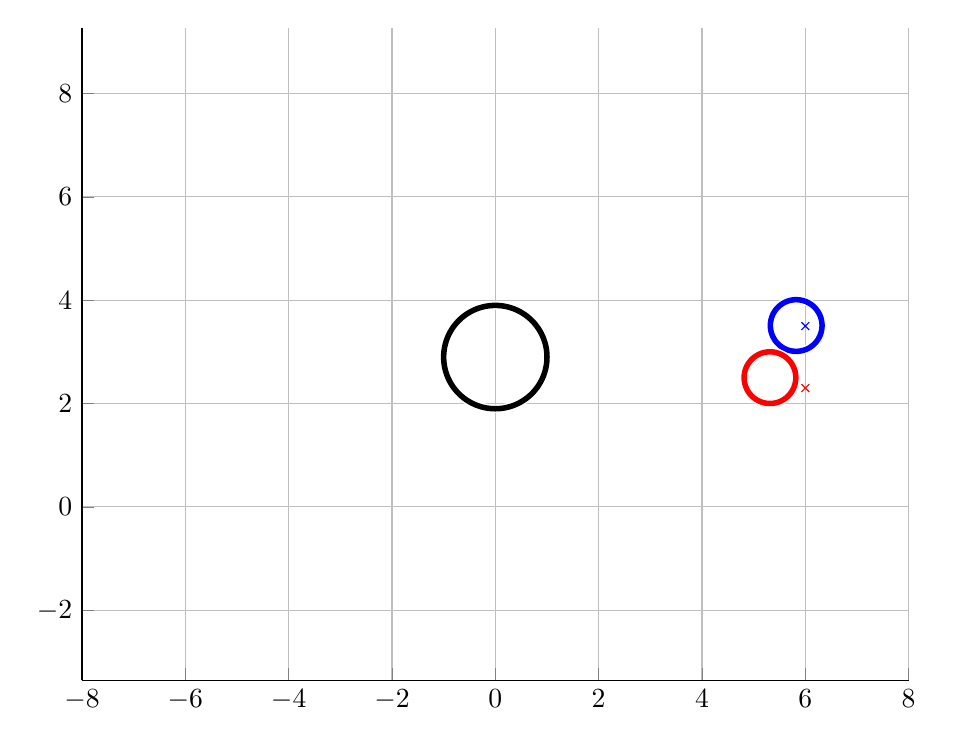
\begin{tikzpicture}

\begin{axis}[%
width=4.133in,
height=3.26in,
at={(0.693in,0.44in)},
scale only axis,
unbounded coords=jump,
xmin=-8,
xmax=8,
xmajorgrids,
ymin=-3.35423843554107,
ymax=9.26511640316861,
ymajorgrids,
axis background/.style={fill=white},
axis x line*=bottom,
axis y line*=left
]
\addplot [color=blue,only marks,mark=x,mark options={solid},forget plot]
  table[row sep=crcr]{%
6	3.5\\
};
\addplot [color=red,only marks,mark=x,mark options={solid},forget plot]
  table[row sep=crcr]{%
6	2.3\\
};
\addplot [color=white,solid,line width=3.0pt,forget plot]
  table[row sep=crcr]{%
6.32403925566145	3.51087796762753\\
6.323734669171	3.52832771597878\\
6.32282128079136	3.5457562044996\\
6.32130020334559	3.56314219926136\\
6.31917329003224	3.58046451810757\\
6.31644313216755	3.597702056461\\
6.31311305602835	3.61483381303641\\
6.30918711879945	3.63183891542737\\
6.30467010363061	3.64869664553603\\
6.29956751380903	3.66538646481501\\
6.2938855660544	3.68188803929037\\
6.28763118294484	3.69818126433549\\
6.28081198448275	3.71424628916543\\
6.27343627881103	3.73006354102207\\
6.26551305209091	3.74561374902048\\
6.25705195755367	3.76087796762753\\
6.24806330373966	3.77583759974414\\
6.23855804193897	3.79047441936291\\
6.22854775284892	3.80477059377377\\
6.21804463246481	3.81870870529036\\
6.20706147722094	3.8322717724708\\
6.19561166840015	3.84544327080696\\
6.18370915583078	3.85820715285703\\
6.17136844089095	3.87054786779686\\
6.15860455884088	3.88245038036623\\
6.14543306050472	3.89390018918702\\
6.13186999332428	3.90488334443089\\
6.11793188180769	3.91538646481501\\
6.10363570739682	3.92539675390505\\
6.08899888777805	3.93490201570575\\
6.07403925566145	3.94389066951975\\
6.0587750370544	3.952351764057\\
6.04322482905599	3.96027499077712\\
6.02740757719935	3.96765069644883\\
6.01134255236941	3.97446989491093\\
5.99504932732428	3.98072427802049\\
5.97854775284892	3.98640622577511\\
5.96185793356995	3.99150881559669\\
5.94500020346128	3.99602583076553\\
5.92799510107033	3.99995176799444\\
5.91086334449492	4.00328184413364\\
5.89362580614148	4.00601200199832\\
5.87630348729528	4.00813891531167\\
5.85891749253351	4.00965999275745\\
5.8414890040127	4.01057338113708\\
5.82403925566145	4.01087796762753\\
5.8065895073102	4.01057338113708\\
5.78916101878939	4.00965999275745\\
5.77177502402762	4.00813891531167\\
5.75445270518142	4.00601200199832\\
5.73721516682799	4.00328184413364\\
5.72008341025257	3.99995176799444\\
5.70307830786162	3.99602583076553\\
5.68622057775295	3.99150881559669\\
5.66953075847398	3.98640622577511\\
5.65302918399862	3.98072427802049\\
5.63673595895349	3.97446989491093\\
5.62067093412355	3.96765069644883\\
5.60485368226691	3.96027499077712\\
5.5893034742685	3.952351764057\\
5.57403925566145	3.94389066951975\\
5.55907962354485	3.93490201570575\\
5.54444280392608	3.92539675390505\\
5.53014662951521	3.91538646481501\\
5.51620851799862	3.90488334443089\\
5.50264545081818	3.89390018918702\\
5.48947395248202	3.88245038036623\\
5.47671007043195	3.87054786779686\\
5.46436935549212	3.85820715285703\\
5.45246684292275	3.84544327080696\\
5.44101703410196	3.8322717724708\\
5.43003387885809	3.81870870529036\\
5.41953075847398	3.80477059377377\\
5.40952046938393	3.79047441936291\\
5.40001520758324	3.77583759974414\\
5.39102655376923	3.76087796762753\\
5.38256545923199	3.74561374902048\\
5.37464223251187	3.73006354102207\\
5.36726652684015	3.71424628916543\\
5.36044732837806	3.69818126433549\\
5.3541929452685	3.68188803929037\\
5.34851099751387	3.66538646481501\\
5.34340840769229	3.64869664553603\\
5.33889139252345	3.63183891542737\\
5.33496545529455	3.61483381303641\\
5.33163537915535	3.597702056461\\
5.32890522129066	3.58046451810757\\
5.32677830797731	3.56314219926136\\
5.32525723053154	3.5457562044996\\
5.3243438421519	3.52832771597878\\
5.32403925566145	3.51087796762753\\
5.3243438421519	3.49342821927628\\
5.32525723053154	3.47599973075547\\
5.32677830797731	3.45861373599371\\
5.32890522129066	3.4412914171475\\
5.33163537915535	3.42405387879407\\
5.33496545529455	3.40692212221865\\
5.33889139252345	3.3899170198277\\
5.34340840769229	3.37305928971903\\
5.34851099751387	3.35636947044006\\
5.3541929452685	3.3398678959647\\
5.36044732837806	3.32357467091958\\
5.36726652684015	3.30750964608963\\
5.37464223251187	3.29169239423299\\
5.38256545923199	3.27614218623459\\
5.39102655376923	3.26087796762753\\
5.40001520758324	3.24591833551093\\
5.40952046938393	3.23128151589216\\
5.41953075847398	3.2169853414813\\
5.43003387885809	3.2030472299647\\
5.44101703410196	3.18948416278426\\
5.45246684292275	3.1763126644481\\
5.46436935549212	3.16354878239803\\
5.47671007043195	3.15120806745821\\
5.48947395248202	3.13930555488884\\
5.50264545081818	3.12785574606804\\
5.51620851799862	3.11687259082417\\
5.53014662951521	3.10636947044006\\
5.54444280392608	3.09635918135001\\
5.55907962354485	3.08685391954932\\
5.57403925566145	3.07786526573531\\
5.5893034742685	3.06940417119807\\
5.60485368226691	3.06148094447795\\
5.62067093412355	3.05410523880623\\
5.63673595895349	3.04728604034414\\
5.65302918399862	3.04103165723458\\
5.66953075847398	3.03534970947996\\
5.68622057775295	3.03024711965837\\
5.70307830786162	3.02573010448953\\
5.72008341025257	3.02180416726063\\
5.73721516682799	3.01847409112143\\
5.75445270518142	3.01574393325675\\
5.77177502402762	3.0136170199434\\
5.78916101878939	3.01209594249762\\
5.8065895073102	3.01118255411799\\
5.82403925566145	3.01087796762753\\
5.8414890040127	3.01118255411799\\
5.85891749253351	3.01209594249762\\
5.87630348729528	3.0136170199434\\
5.89362580614148	3.01574393325675\\
5.91086334449492	3.01847409112143\\
5.92799510107033	3.02180416726063\\
5.94500020346128	3.02573010448953\\
5.96185793356995	3.03024711965837\\
5.97854775284892	3.03534970947996\\
5.99504932732428	3.04103165723458\\
6.01134255236941	3.04728604034414\\
6.02740757719935	3.05410523880623\\
6.04322482905599	3.06148094447795\\
6.0587750370544	3.06940417119807\\
6.07403925566145	3.07786526573531\\
6.08899888777805	3.08685391954932\\
6.10363570739682	3.09635918135001\\
6.11793188180769	3.10636947044006\\
6.13186999332428	3.11687259082417\\
6.14543306050472	3.12785574606804\\
6.15860455884088	3.13930555488884\\
6.17136844089095	3.15120806745821\\
6.18370915583078	3.16354878239803\\
6.19561166840015	3.1763126644481\\
6.20706147722094	3.18948416278426\\
6.21804463246481	3.2030472299647\\
6.22854775284892	3.2169853414813\\
6.23855804193897	3.23128151589216\\
6.24806330373966	3.24591833551093\\
6.25705195755367	3.26087796762753\\
6.26551305209091	3.27614218623459\\
6.27343627881103	3.29169239423299\\
6.28081198448275	3.30750964608963\\
6.28763118294484	3.32357467091958\\
6.2938855660544	3.3398678959647\\
6.29956751380903	3.35636947044006\\
6.30467010363061	3.37305928971903\\
6.30918711879945	3.3899170198277\\
6.31311305602835	3.40692212221865\\
6.31644313216755	3.42405387879407\\
6.31917329003224	3.4412914171475\\
6.32130020334559	3.45861373599371\\
6.32282128079136	3.47599973075547\\
6.323734669171	3.49342821927628\\
6.32403925566145	3.51087796762753\\
nan	nan\\
};
\addplot [color=blue,solid,line width=2.0pt,forget plot]
  table[row sep=crcr]{%
6.32403925566145	3.51087796762753\\
6.323734669171	3.52832771597878\\
6.32282128079136	3.5457562044996\\
6.32130020334559	3.56314219926136\\
6.31917329003224	3.58046451810757\\
6.31644313216755	3.597702056461\\
6.31311305602835	3.61483381303641\\
6.30918711879945	3.63183891542737\\
6.30467010363061	3.64869664553603\\
6.29956751380903	3.66538646481501\\
6.2938855660544	3.68188803929037\\
6.28763118294484	3.69818126433549\\
6.28081198448275	3.71424628916543\\
6.27343627881103	3.73006354102207\\
6.26551305209091	3.74561374902048\\
6.25705195755367	3.76087796762753\\
6.24806330373966	3.77583759974414\\
6.23855804193897	3.79047441936291\\
6.22854775284892	3.80477059377377\\
6.21804463246481	3.81870870529036\\
6.20706147722094	3.8322717724708\\
6.19561166840015	3.84544327080696\\
6.18370915583078	3.85820715285703\\
6.17136844089095	3.87054786779686\\
6.15860455884088	3.88245038036623\\
6.14543306050472	3.89390018918702\\
6.13186999332428	3.90488334443089\\
6.11793188180769	3.91538646481501\\
6.10363570739682	3.92539675390505\\
6.08899888777805	3.93490201570575\\
6.07403925566145	3.94389066951975\\
6.0587750370544	3.952351764057\\
6.04322482905599	3.96027499077712\\
6.02740757719935	3.96765069644883\\
6.01134255236941	3.97446989491093\\
5.99504932732428	3.98072427802049\\
5.97854775284892	3.98640622577511\\
5.96185793356995	3.99150881559669\\
5.94500020346128	3.99602583076553\\
5.92799510107033	3.99995176799444\\
5.91086334449492	4.00328184413364\\
5.89362580614148	4.00601200199832\\
5.87630348729528	4.00813891531167\\
5.85891749253351	4.00965999275745\\
5.8414890040127	4.01057338113708\\
5.82403925566145	4.01087796762753\\
5.8065895073102	4.01057338113708\\
5.78916101878939	4.00965999275745\\
5.77177502402762	4.00813891531167\\
5.75445270518142	4.00601200199832\\
5.73721516682799	4.00328184413364\\
5.72008341025257	3.99995176799444\\
5.70307830786162	3.99602583076553\\
5.68622057775295	3.99150881559669\\
5.66953075847398	3.98640622577511\\
5.65302918399862	3.98072427802049\\
5.63673595895349	3.97446989491093\\
5.62067093412355	3.96765069644883\\
5.60485368226691	3.96027499077712\\
5.5893034742685	3.952351764057\\
5.57403925566145	3.94389066951975\\
5.55907962354485	3.93490201570575\\
5.54444280392608	3.92539675390505\\
5.53014662951521	3.91538646481501\\
5.51620851799862	3.90488334443089\\
5.50264545081818	3.89390018918702\\
5.48947395248202	3.88245038036623\\
5.47671007043195	3.87054786779686\\
5.46436935549212	3.85820715285703\\
5.45246684292275	3.84544327080696\\
5.44101703410196	3.8322717724708\\
5.43003387885809	3.81870870529036\\
5.41953075847398	3.80477059377377\\
5.40952046938393	3.79047441936291\\
5.40001520758324	3.77583759974414\\
5.39102655376923	3.76087796762753\\
5.38256545923199	3.74561374902048\\
5.37464223251187	3.73006354102207\\
5.36726652684015	3.71424628916543\\
5.36044732837806	3.69818126433549\\
5.3541929452685	3.68188803929037\\
5.34851099751387	3.66538646481501\\
5.34340840769229	3.64869664553603\\
5.33889139252345	3.63183891542737\\
5.33496545529455	3.61483381303641\\
5.33163537915535	3.597702056461\\
5.32890522129066	3.58046451810757\\
5.32677830797731	3.56314219926136\\
5.32525723053154	3.5457562044996\\
5.3243438421519	3.52832771597878\\
5.32403925566145	3.51087796762753\\
5.3243438421519	3.49342821927628\\
5.32525723053154	3.47599973075547\\
5.32677830797731	3.45861373599371\\
5.32890522129066	3.4412914171475\\
5.33163537915535	3.42405387879407\\
5.33496545529455	3.40692212221865\\
5.33889139252345	3.3899170198277\\
5.34340840769229	3.37305928971903\\
5.34851099751387	3.35636947044006\\
5.3541929452685	3.3398678959647\\
5.36044732837806	3.32357467091958\\
5.36726652684015	3.30750964608963\\
5.37464223251187	3.29169239423299\\
5.38256545923199	3.27614218623459\\
5.39102655376923	3.26087796762753\\
5.40001520758324	3.24591833551093\\
5.40952046938393	3.23128151589216\\
5.41953075847398	3.2169853414813\\
5.43003387885809	3.2030472299647\\
5.44101703410196	3.18948416278426\\
5.45246684292275	3.1763126644481\\
5.46436935549212	3.16354878239803\\
5.47671007043195	3.15120806745821\\
5.48947395248202	3.13930555488884\\
5.50264545081818	3.12785574606804\\
5.51620851799862	3.11687259082417\\
5.53014662951521	3.10636947044006\\
5.54444280392608	3.09635918135001\\
5.55907962354485	3.08685391954932\\
5.57403925566145	3.07786526573531\\
5.5893034742685	3.06940417119807\\
5.60485368226691	3.06148094447795\\
5.62067093412355	3.05410523880623\\
5.63673595895349	3.04728604034414\\
5.65302918399862	3.04103165723458\\
5.66953075847398	3.03534970947996\\
5.68622057775295	3.03024711965837\\
5.70307830786162	3.02573010448953\\
5.72008341025257	3.02180416726063\\
5.73721516682799	3.01847409112143\\
5.75445270518142	3.01574393325675\\
5.77177502402762	3.0136170199434\\
5.78916101878939	3.01209594249762\\
5.8065895073102	3.01118255411799\\
5.82403925566145	3.01087796762753\\
5.8414890040127	3.01118255411799\\
5.85891749253351	3.01209594249762\\
5.87630348729528	3.0136170199434\\
5.89362580614148	3.01574393325675\\
5.91086334449492	3.01847409112143\\
5.92799510107033	3.02180416726063\\
5.94500020346128	3.02573010448953\\
5.96185793356995	3.03024711965837\\
5.97854775284892	3.03534970947996\\
5.99504932732428	3.04103165723458\\
6.01134255236941	3.04728604034414\\
6.02740757719935	3.05410523880623\\
6.04322482905599	3.06148094447795\\
6.0587750370544	3.06940417119807\\
6.07403925566145	3.07786526573531\\
6.08899888777805	3.08685391954932\\
6.10363570739682	3.09635918135001\\
6.11793188180769	3.10636947044006\\
6.13186999332428	3.11687259082417\\
6.14543306050472	3.12785574606804\\
6.15860455884088	3.13930555488884\\
6.17136844089095	3.15120806745821\\
6.18370915583078	3.16354878239803\\
6.19561166840015	3.1763126644481\\
6.20706147722094	3.18948416278426\\
6.21804463246481	3.2030472299647\\
6.22854775284892	3.2169853414813\\
6.23855804193897	3.23128151589216\\
6.24806330373966	3.24591833551093\\
6.25705195755367	3.26087796762753\\
6.26551305209091	3.27614218623459\\
6.27343627881103	3.29169239423299\\
6.28081198448275	3.30750964608963\\
6.28763118294484	3.32357467091958\\
6.2938855660544	3.3398678959647\\
6.29956751380903	3.35636947044006\\
6.30467010363061	3.37305928971903\\
6.30918711879945	3.3899170198277\\
6.31311305602835	3.40692212221865\\
6.31644313216755	3.42405387879407\\
6.31917329003224	3.4412914171475\\
6.32130020334559	3.45861373599371\\
6.32282128079136	3.47599973075547\\
6.323734669171	3.49342821927628\\
6.32403925566145	3.51087796762753\\
nan	nan\\
};
\addplot [color=white,solid,line width=3.0pt,forget plot]
  table[row sep=crcr]{%
5.81624308249222	2.50193568652253\\
5.81593849600177	2.51938543487378\\
5.81502510762213	2.53681392339459\\
5.81350403017635	2.55419991815635\\
5.811377116863	2.57152223700256\\
5.80864695899832	2.58875977535599\\
5.80531688285912	2.60589153193141\\
5.80139094563022	2.62289663432236\\
5.79687393046138	2.63975436443103\\
5.7917713406398	2.65644418371\\
5.78608939288517	2.67294575818536\\
5.77983500977561	2.68923898323048\\
5.77301581131352	2.70530400806043\\
5.7656401056418	2.72112125991706\\
5.75771687892168	2.73667146791547\\
5.74925578438444	2.75193568652253\\
5.74026713057043	2.76689531863913\\
5.73076186876974	2.7815321382579\\
5.72075157967969	2.79582831266876\\
5.71024845929558	2.80976642418536\\
5.69926530405171	2.8233294913658\\
5.68781549523092	2.83650098970196\\
5.67591298266154	2.84926487175203\\
5.66357226772172	2.86160558669185\\
5.65080838567165	2.87350809926122\\
5.63763688733549	2.88495790808202\\
5.62407382015505	2.89594106332589\\
5.61013570863846	2.90644418371\\
5.59583953422759	2.91645447280005\\
5.58120271460882	2.92595973460074\\
5.56624308249222	2.93494838841475\\
5.55097886388516	2.94340948295199\\
5.53542865588676	2.95133270967211\\
5.51961140403012	2.95870841534383\\
5.50354637920017	2.96552761380592\\
5.48725315415505	2.97178199691548\\
5.47075157967969	2.9774639446701\\
5.45406176040072	2.98256653449169\\
5.43720403029205	2.98708354966052\\
5.4201989279011	2.99100948688943\\
5.40306717132568	2.99433956302863\\
5.38582963297225	2.99706972089331\\
5.36850731412605	2.99919663420666\\
5.35112131936428	3.00071771165244\\
5.33369283084347	3.00163110003207\\
5.31624308249222	3.00193568652253\\
5.29879333414097	3.00163110003207\\
5.28136484562016	3.00071771165244\\
5.26397885085839	2.99919663420666\\
5.24665653201219	2.99706972089331\\
5.22941899365875	2.99433956302863\\
5.21228723708334	2.99100948688943\\
5.19528213469238	2.98708354966052\\
5.17842440458372	2.98256653449169\\
5.16173458530475	2.9774639446701\\
5.14523301082938	2.97178199691548\\
5.12893978578426	2.96552761380592\\
5.11287476095432	2.95870841534383\\
5.09705750909768	2.95133270967211\\
5.08150730109927	2.94340948295199\\
5.06624308249222	2.93494838841475\\
5.05128345037562	2.92595973460074\\
5.03664663075685	2.91645447280005\\
5.02235045634598	2.90644418371\\
5.00841234482939	2.89594106332589\\
4.99484927764895	2.88495790808202\\
4.98167777931279	2.87350809926122\\
4.96891389726272	2.86160558669185\\
4.95657318232289	2.84926487175203\\
4.94467066975352	2.83650098970196\\
4.93322086093273	2.8233294913658\\
4.92223770568886	2.80976642418536\\
4.91173458530475	2.79582831266876\\
4.9017242962147	2.7815321382579\\
4.89221903441401	2.76689531863913\\
4.8832303806	2.75193568652253\\
4.87476928606276	2.73667146791547\\
4.86684605934263	2.72112125991706\\
4.85947035367092	2.70530400806043\\
4.85265115520883	2.68923898323048\\
4.84639677209926	2.67294575818536\\
4.84071482434464	2.65644418371\\
4.83561223452306	2.63975436443103\\
4.83109521935422	2.62289663432236\\
4.82716928212532	2.60589153193141\\
4.82383920598611	2.58875977535599\\
4.82110904812143	2.57152223700256\\
4.81898213480808	2.55419991815635\\
4.81746105736231	2.53681392339459\\
4.81654766898267	2.51938543487378\\
4.81624308249222	2.50193568652253\\
4.81654766898267	2.48448593817128\\
4.81746105736231	2.46705744965046\\
4.81898213480808	2.4496714548887\\
4.82110904812143	2.43234913604249\\
4.82383920598611	2.41511159768906\\
4.82716928212532	2.39797984111365\\
4.83109521935422	2.38097473872269\\
4.83561223452306	2.36411700861403\\
4.84071482434464	2.34742718933505\\
4.84639677209926	2.33092561485969\\
4.85265115520883	2.31463238981457\\
4.85947035367092	2.29856736498463\\
4.86684605934263	2.28275011312799\\
4.87476928606276	2.26719990512958\\
4.8832303806	2.25193568652253\\
4.89221903441401	2.23697605440592\\
4.9017242962147	2.22233923478715\\
4.91173458530474	2.20804306037629\\
4.92223770568886	2.1941049488597\\
4.93322086093273	2.18054188167926\\
4.94467066975352	2.1673703833431\\
4.95657318232289	2.15460650129303\\
4.96891389726272	2.1422657863532\\
4.98167777931279	2.13036327378383\\
4.99484927764895	2.11891346496304\\
5.00841234482939	2.10793030971917\\
5.02235045634598	2.09742718933505\\
5.03664663075685	2.08741690024501\\
5.05128345037562	2.07791163844431\\
5.06624308249222	2.06892298463031\\
5.08150730109927	2.06046189009306\\
5.09705750909768	2.05253866337294\\
5.11287476095432	2.04516295770123\\
5.12893978578426	2.03834375923913\\
5.14523301082938	2.03208937612957\\
5.16173458530474	2.02640742837495\\
5.17842440458372	2.02130483855337\\
5.19528213469238	2.01678782338453\\
5.21228723708334	2.01286188615562\\
5.22941899365875	2.00953181001642\\
5.24665653201219	2.00680165215174\\
5.26397885085839	2.00467473883839\\
5.28136484562016	2.00315366139261\\
5.29879333414097	2.00224027301298\\
5.31624308249222	2.00193568652253\\
5.33369283084347	2.00224027301298\\
5.35112131936428	2.00315366139261\\
5.36850731412605	2.00467473883839\\
5.38582963297225	2.00680165215174\\
5.40306717132568	2.00953181001642\\
5.4201989279011	2.01286188615562\\
5.43720403029205	2.01678782338453\\
5.45406176040072	2.02130483855337\\
5.47075157967969	2.02640742837495\\
5.48725315415505	2.03208937612957\\
5.50354637920017	2.03834375923913\\
5.51961140403012	2.04516295770123\\
5.53542865588676	2.05253866337294\\
5.55097886388516	2.06046189009306\\
5.56624308249222	2.06892298463031\\
5.58120271460882	2.07791163844431\\
5.59583953422759	2.08741690024501\\
5.61013570863846	2.09742718933505\\
5.62407382015505	2.10793030971917\\
5.63763688733549	2.11891346496304\\
5.65080838567165	2.13036327378383\\
5.66357226772172	2.1422657863532\\
5.67591298266154	2.15460650129303\\
5.68781549523092	2.1673703833431\\
5.69926530405171	2.18054188167926\\
5.71024845929558	2.1941049488597\\
5.72075157967969	2.20804306037629\\
5.73076186876974	2.22233923478715\\
5.74026713057043	2.23697605440592\\
5.74925578438444	2.25193568652253\\
5.75771687892168	2.26719990512958\\
5.7656401056418	2.28275011312799\\
5.77301581131352	2.29856736498463\\
5.77983500977561	2.31463238981457\\
5.78608939288517	2.33092561485969\\
5.7917713406398	2.34742718933505\\
5.79687393046138	2.36411700861403\\
5.80139094563022	2.38097473872269\\
5.80531688285912	2.39797984111365\\
5.80864695899832	2.41511159768906\\
5.811377116863	2.43234913604249\\
5.81350403017635	2.4496714548887\\
5.81502510762213	2.46705744965046\\
5.81593849600177	2.48448593817128\\
5.81624308249222	2.50193568652253\\
nan	nan\\
};
\addplot [color=red,solid,line width=2.0pt,forget plot]
  table[row sep=crcr]{%
5.81624308249222	2.50193568652253\\
5.81593849600177	2.51938543487378\\
5.81502510762213	2.53681392339459\\
5.81350403017635	2.55419991815635\\
5.811377116863	2.57152223700256\\
5.80864695899832	2.58875977535599\\
5.80531688285912	2.60589153193141\\
5.80139094563022	2.62289663432236\\
5.79687393046138	2.63975436443103\\
5.7917713406398	2.65644418371\\
5.78608939288517	2.67294575818536\\
5.77983500977561	2.68923898323048\\
5.77301581131352	2.70530400806043\\
5.7656401056418	2.72112125991706\\
5.75771687892168	2.73667146791547\\
5.74925578438444	2.75193568652253\\
5.74026713057043	2.76689531863913\\
5.73076186876974	2.7815321382579\\
5.72075157967969	2.79582831266876\\
5.71024845929558	2.80976642418536\\
5.69926530405171	2.8233294913658\\
5.68781549523092	2.83650098970196\\
5.67591298266154	2.84926487175203\\
5.66357226772172	2.86160558669185\\
5.65080838567165	2.87350809926122\\
5.63763688733549	2.88495790808202\\
5.62407382015505	2.89594106332589\\
5.61013570863846	2.90644418371\\
5.59583953422759	2.91645447280005\\
5.58120271460882	2.92595973460074\\
5.56624308249222	2.93494838841475\\
5.55097886388516	2.94340948295199\\
5.53542865588676	2.95133270967211\\
5.51961140403012	2.95870841534383\\
5.50354637920017	2.96552761380592\\
5.48725315415505	2.97178199691548\\
5.47075157967969	2.9774639446701\\
5.45406176040072	2.98256653449169\\
5.43720403029205	2.98708354966052\\
5.4201989279011	2.99100948688943\\
5.40306717132568	2.99433956302863\\
5.38582963297225	2.99706972089331\\
5.36850731412605	2.99919663420666\\
5.35112131936428	3.00071771165244\\
5.33369283084347	3.00163110003207\\
5.31624308249222	3.00193568652253\\
5.29879333414097	3.00163110003207\\
5.28136484562016	3.00071771165244\\
5.26397885085839	2.99919663420666\\
5.24665653201219	2.99706972089331\\
5.22941899365875	2.99433956302863\\
5.21228723708334	2.99100948688943\\
5.19528213469238	2.98708354966052\\
5.17842440458372	2.98256653449169\\
5.16173458530475	2.9774639446701\\
5.14523301082938	2.97178199691548\\
5.12893978578426	2.96552761380592\\
5.11287476095432	2.95870841534383\\
5.09705750909768	2.95133270967211\\
5.08150730109927	2.94340948295199\\
5.06624308249222	2.93494838841475\\
5.05128345037562	2.92595973460074\\
5.03664663075685	2.91645447280005\\
5.02235045634598	2.90644418371\\
5.00841234482939	2.89594106332589\\
4.99484927764895	2.88495790808202\\
4.98167777931279	2.87350809926122\\
4.96891389726272	2.86160558669185\\
4.95657318232289	2.84926487175203\\
4.94467066975352	2.83650098970196\\
4.93322086093273	2.8233294913658\\
4.92223770568886	2.80976642418536\\
4.91173458530475	2.79582831266876\\
4.9017242962147	2.7815321382579\\
4.89221903441401	2.76689531863913\\
4.8832303806	2.75193568652253\\
4.87476928606276	2.73667146791547\\
4.86684605934263	2.72112125991706\\
4.85947035367092	2.70530400806043\\
4.85265115520883	2.68923898323048\\
4.84639677209926	2.67294575818536\\
4.84071482434464	2.65644418371\\
4.83561223452306	2.63975436443103\\
4.83109521935422	2.62289663432236\\
4.82716928212532	2.60589153193141\\
4.82383920598611	2.58875977535599\\
4.82110904812143	2.57152223700256\\
4.81898213480808	2.55419991815635\\
4.81746105736231	2.53681392339459\\
4.81654766898267	2.51938543487378\\
4.81624308249222	2.50193568652253\\
4.81654766898267	2.48448593817128\\
4.81746105736231	2.46705744965046\\
4.81898213480808	2.4496714548887\\
4.82110904812143	2.43234913604249\\
4.82383920598611	2.41511159768906\\
4.82716928212532	2.39797984111365\\
4.83109521935422	2.38097473872269\\
4.83561223452306	2.36411700861403\\
4.84071482434464	2.34742718933505\\
4.84639677209926	2.33092561485969\\
4.85265115520883	2.31463238981457\\
4.85947035367092	2.29856736498463\\
4.86684605934263	2.28275011312799\\
4.87476928606276	2.26719990512958\\
4.8832303806	2.25193568652253\\
4.89221903441401	2.23697605440592\\
4.9017242962147	2.22233923478715\\
4.91173458530474	2.20804306037629\\
4.92223770568886	2.1941049488597\\
4.93322086093273	2.18054188167926\\
4.94467066975352	2.1673703833431\\
4.95657318232289	2.15460650129303\\
4.96891389726272	2.1422657863532\\
4.98167777931279	2.13036327378383\\
4.99484927764895	2.11891346496304\\
5.00841234482939	2.10793030971917\\
5.02235045634598	2.09742718933505\\
5.03664663075685	2.08741690024501\\
5.05128345037562	2.07791163844431\\
5.06624308249222	2.06892298463031\\
5.08150730109927	2.06046189009306\\
5.09705750909768	2.05253866337294\\
5.11287476095432	2.04516295770123\\
5.12893978578426	2.03834375923913\\
5.14523301082938	2.03208937612957\\
5.16173458530474	2.02640742837495\\
5.17842440458372	2.02130483855337\\
5.19528213469238	2.01678782338453\\
5.21228723708334	2.01286188615562\\
5.22941899365875	2.00953181001642\\
5.24665653201219	2.00680165215174\\
5.26397885085839	2.00467473883839\\
5.28136484562016	2.00315366139261\\
5.29879333414097	2.00224027301298\\
5.31624308249222	2.00193568652253\\
5.33369283084347	2.00224027301298\\
5.35112131936428	2.00315366139261\\
5.36850731412605	2.00467473883839\\
5.38582963297225	2.00680165215174\\
5.40306717132568	2.00953181001642\\
5.4201989279011	2.01286188615562\\
5.43720403029205	2.01678782338453\\
5.45406176040072	2.02130483855337\\
5.47075157967969	2.02640742837495\\
5.48725315415505	2.03208937612957\\
5.50354637920017	2.03834375923913\\
5.51961140403012	2.04516295770123\\
5.53542865588676	2.05253866337294\\
5.55097886388516	2.06046189009306\\
5.56624308249222	2.06892298463031\\
5.58120271460882	2.07791163844431\\
5.59583953422759	2.08741690024501\\
5.61013570863846	2.09742718933505\\
5.62407382015505	2.10793030971917\\
5.63763688733549	2.11891346496304\\
5.65080838567165	2.13036327378383\\
5.66357226772172	2.1422657863532\\
5.67591298266154	2.15460650129303\\
5.68781549523092	2.1673703833431\\
5.69926530405171	2.18054188167926\\
5.71024845929558	2.1941049488597\\
5.72075157967969	2.20804306037629\\
5.73076186876974	2.22233923478715\\
5.74026713057043	2.23697605440592\\
5.74925578438444	2.25193568652253\\
5.75771687892168	2.26719990512958\\
5.7656401056418	2.28275011312799\\
5.77301581131352	2.29856736498463\\
5.77983500977561	2.31463238981457\\
5.78608939288517	2.33092561485969\\
5.7917713406398	2.34742718933505\\
5.79687393046138	2.36411700861403\\
5.80139094563022	2.38097473872269\\
5.80531688285912	2.39797984111365\\
5.80864695899832	2.41511159768906\\
5.811377116863	2.43234913604249\\
5.81350403017635	2.4496714548887\\
5.81502510762213	2.46705744965046\\
5.81593849600177	2.48448593817128\\
5.81624308249222	2.50193568652253\\
nan	nan\\
};
\addplot [color=white,solid,line width=3.0pt,forget plot]
  table[row sep=crcr]{%
1	2.9\\
0.999390827019096	2.9348994967025\\
0.997564050259824	2.96975647374413\\
0.994521895368273	3.00452846326765\\
0.99026806874157	3.03917310096007\\
0.984807753012208	3.07364817766693\\
0.978147600733806	3.10791169081776\\
0.970295726275996	3.14192189559967\\
0.961261695938319	3.175637355817\\
0.951056516295154	3.20901699437495\\
0.939692620785908	3.24202014332567\\
0.927183854566787	3.27460659341591\\
0.913545457642601	3.3067366430758\\
0.898794046299167	3.33837114678908\\
0.882947592858927	3.36947156278589\\
0.866025403784439	3.4\\
0.848048096156426	3.42991926423321\\
0.829037572555042	3.45919290347075\\
0.809016994374947	3.48778525229247\\
0.788010753606722	3.51566147532566\\
0.766044443118978	3.54278760968654\\
0.743144825477394	3.56913060635886\\
0.719339800338651	3.594658370459\\
0.694658370458997	3.61933980033865\\
0.669130606358858	3.64314482547739\\
0.642787609686539	3.66604444311898\\
0.615661475325658	3.68801075360672\\
0.587785252292473	3.70901699437495\\
0.559192903470747	3.72903757255504\\
0.529919264233205	3.74804809615643\\
0.5	3.76602540378444\\
0.469471562785891	3.78294759285893\\
0.438371146789077	3.79879404629917\\
0.4067366430758	3.8135454576426\\
0.374606593415912	3.82718385456679\\
0.342020143325669	3.83969262078591\\
0.309016994374947	3.85105651629515\\
0.275637355816999	3.86126169593832\\
0.241921895599668	3.870295726276\\
0.207911690817759	3.87814760073381\\
0.17364817766693	3.88480775301221\\
0.139173100960066	3.89026806874157\\
0.104528463267653	3.89452189536827\\
0.0697564737441255	3.89756405025982\\
0.0348994967025011	3.8993908270191\\
6.12323399573677e-17	3.9\\
-0.0348994967025007	3.8993908270191\\
-0.0697564737441253	3.89756405025982\\
-0.104528463267653	3.89452189536827\\
-0.139173100960065	3.89026806874157\\
-0.17364817766693	3.88480775301221\\
-0.207911690817759	3.87814760073381\\
-0.241921895599668	3.870295726276\\
-0.275637355816999	3.86126169593832\\
-0.309016994374947	3.85105651629515\\
-0.342020143325669	3.83969262078591\\
-0.374606593415912	3.82718385456679\\
-0.4067366430758	3.8135454576426\\
-0.438371146789078	3.79879404629917\\
-0.469471562785891	3.78294759285893\\
-0.5	3.76602540378444\\
-0.529919264233205	3.74804809615643\\
-0.559192903470747	3.72903757255504\\
-0.587785252292473	3.70901699437495\\
-0.615661475325658	3.68801075360672\\
-0.642787609686539	3.66604444311898\\
-0.669130606358858	3.64314482547739\\
-0.694658370458997	3.61933980033865\\
-0.719339800338651	3.594658370459\\
-0.743144825477394	3.56913060635886\\
-0.766044443118978	3.54278760968654\\
-0.788010753606722	3.51566147532566\\
-0.809016994374947	3.48778525229247\\
-0.829037572555042	3.45919290347075\\
-0.848048096156426	3.42991926423321\\
-0.866025403784439	3.4\\
-0.882947592858927	3.36947156278589\\
-0.898794046299167	3.33837114678908\\
-0.913545457642601	3.3067366430758\\
-0.927183854566787	3.27460659341591\\
-0.939692620785908	3.24202014332567\\
-0.951056516295154	3.20901699437495\\
-0.961261695938319	3.175637355817\\
-0.970295726275996	3.14192189559967\\
-0.978147600733806	3.10791169081776\\
-0.984807753012208	3.07364817766693\\
-0.99026806874157	3.03917310096007\\
-0.994521895368273	3.00452846326765\\
-0.997564050259824	2.96975647374413\\
-0.999390827019096	2.9348994967025\\
-1	2.9\\
-0.999390827019096	2.8651005032975\\
-0.997564050259824	2.83024352625588\\
-0.994521895368273	2.79547153673235\\
-0.99026806874157	2.76082689903993\\
-0.984807753012208	2.72635182233307\\
-0.978147600733806	2.69208830918224\\
-0.970295726275997	2.65807810440033\\
-0.961261695938319	2.624362644183\\
-0.951056516295154	2.59098300562505\\
-0.939692620785908	2.55797985667433\\
-0.927183854566787	2.52539340658409\\
-0.913545457642601	2.4932633569242\\
-0.898794046299167	2.46162885321092\\
-0.882947592858927	2.43052843721411\\
-0.866025403784439	2.4\\
-0.848048096156426	2.3700807357668\\
-0.829037572555042	2.34080709652925\\
-0.809016994374947	2.31221474770753\\
-0.788010753606722	2.28433852467434\\
-0.766044443118978	2.25721239031346\\
-0.743144825477394	2.23086939364114\\
-0.719339800338651	2.205341629541\\
-0.694658370458997	2.18066019966135\\
-0.669130606358858	2.15685517452261\\
-0.642787609686539	2.13395555688102\\
-0.615661475325658	2.11198924639328\\
-0.587785252292473	2.09098300562505\\
-0.559192903470747	2.07096242744496\\
-0.529919264233205	2.05195190384357\\
-0.5	2.03397459621556\\
-0.469471562785891	2.01705240714107\\
-0.438371146789078	2.00120595370083\\
-0.4067366430758	1.9864545423574\\
-0.374606593415912	1.97281614543321\\
-0.342020143325669	1.96030737921409\\
-0.309016994374948	1.94894348370485\\
-0.275637355816999	1.93873830406168\\
-0.241921895599668	1.929704273724\\
-0.20791169081776	1.92185239926619\\
-0.17364817766693	1.91519224698779\\
-0.139173100960065	1.90973193125843\\
-0.104528463267653	1.90547810463173\\
-0.0697564737441256	1.90243594974018\\
-0.0348994967025016	1.9006091729809\\
-1.83697019872103e-16	1.9\\
0.0348994967025013	1.9006091729809\\
0.0697564737441252	1.90243594974018\\
0.104528463267653	1.90547810463173\\
0.139173100960065	1.90973193125843\\
0.17364817766693	1.91519224698779\\
0.207911690817759	1.92185239926619\\
0.241921895599667	1.929704273724\\
0.275637355816999	1.93873830406168\\
0.309016994374947	1.94894348370485\\
0.342020143325668	1.96030737921409\\
0.374606593415912	1.97281614543321\\
0.406736643075801	1.9864545423574\\
0.438371146789077	2.00120595370083\\
0.46947156278589	2.01705240714107\\
0.5	2.03397459621556\\
0.529919264233205	2.05195190384357\\
0.559192903470746	2.07096242744496\\
0.587785252292473	2.09098300562505\\
0.615661475325659	2.11198924639328\\
0.642787609686539	2.13395555688102\\
0.669130606358858	2.15685517452261\\
0.694658370458997	2.18066019966135\\
0.719339800338651	2.205341629541\\
0.743144825477394	2.23086939364114\\
0.766044443118978	2.25721239031346\\
0.788010753606722	2.28433852467434\\
0.809016994374947	2.31221474770753\\
0.829037572555041	2.34080709652925\\
0.848048096156425	2.37008073576679\\
0.866025403784438	2.4\\
0.882947592858927	2.43052843721411\\
0.898794046299167	2.46162885321092\\
0.913545457642601	2.4932633569242\\
0.927183854566787	2.52539340658409\\
0.939692620785908	2.55797985667433\\
0.951056516295154	2.59098300562505\\
0.961261695938319	2.624362644183\\
0.970295726275996	2.65807810440033\\
0.978147600733806	2.69208830918224\\
0.984807753012208	2.72635182233307\\
0.99026806874157	2.76082689903993\\
0.994521895368273	2.79547153673235\\
0.997564050259824	2.83024352625588\\
0.999390827019096	2.8651005032975\\
1	2.9\\
nan	nan\\
};
\addplot [color=black,solid,line width=2.0pt,forget plot]
  table[row sep=crcr]{%
1	2.9\\
0.999390827019096	2.9348994967025\\
0.997564050259824	2.96975647374413\\
0.994521895368273	3.00452846326765\\
0.99026806874157	3.03917310096007\\
0.984807753012208	3.07364817766693\\
0.978147600733806	3.10791169081776\\
0.970295726275996	3.14192189559967\\
0.961261695938319	3.175637355817\\
0.951056516295154	3.20901699437495\\
0.939692620785908	3.24202014332567\\
0.927183854566787	3.27460659341591\\
0.913545457642601	3.3067366430758\\
0.898794046299167	3.33837114678908\\
0.882947592858927	3.36947156278589\\
0.866025403784439	3.4\\
0.848048096156426	3.42991926423321\\
0.829037572555042	3.45919290347075\\
0.809016994374947	3.48778525229247\\
0.788010753606722	3.51566147532566\\
0.766044443118978	3.54278760968654\\
0.743144825477394	3.56913060635886\\
0.719339800338651	3.594658370459\\
0.694658370458997	3.61933980033865\\
0.669130606358858	3.64314482547739\\
0.642787609686539	3.66604444311898\\
0.615661475325658	3.68801075360672\\
0.587785252292473	3.70901699437495\\
0.559192903470747	3.72903757255504\\
0.529919264233205	3.74804809615643\\
0.5	3.76602540378444\\
0.469471562785891	3.78294759285893\\
0.438371146789077	3.79879404629917\\
0.4067366430758	3.8135454576426\\
0.374606593415912	3.82718385456679\\
0.342020143325669	3.83969262078591\\
0.309016994374947	3.85105651629515\\
0.275637355816999	3.86126169593832\\
0.241921895599668	3.870295726276\\
0.207911690817759	3.87814760073381\\
0.17364817766693	3.88480775301221\\
0.139173100960066	3.89026806874157\\
0.104528463267653	3.89452189536827\\
0.0697564737441255	3.89756405025982\\
0.0348994967025011	3.8993908270191\\
6.12323399573677e-17	3.9\\
-0.0348994967025007	3.8993908270191\\
-0.0697564737441253	3.89756405025982\\
-0.104528463267653	3.89452189536827\\
-0.139173100960065	3.89026806874157\\
-0.17364817766693	3.88480775301221\\
-0.207911690817759	3.87814760073381\\
-0.241921895599668	3.870295726276\\
-0.275637355816999	3.86126169593832\\
-0.309016994374947	3.85105651629515\\
-0.342020143325669	3.83969262078591\\
-0.374606593415912	3.82718385456679\\
-0.4067366430758	3.8135454576426\\
-0.438371146789078	3.79879404629917\\
-0.469471562785891	3.78294759285893\\
-0.5	3.76602540378444\\
-0.529919264233205	3.74804809615643\\
-0.559192903470747	3.72903757255504\\
-0.587785252292473	3.70901699437495\\
-0.615661475325658	3.68801075360672\\
-0.642787609686539	3.66604444311898\\
-0.669130606358858	3.64314482547739\\
-0.694658370458997	3.61933980033865\\
-0.719339800338651	3.594658370459\\
-0.743144825477394	3.56913060635886\\
-0.766044443118978	3.54278760968654\\
-0.788010753606722	3.51566147532566\\
-0.809016994374947	3.48778525229247\\
-0.829037572555042	3.45919290347075\\
-0.848048096156426	3.42991926423321\\
-0.866025403784439	3.4\\
-0.882947592858927	3.36947156278589\\
-0.898794046299167	3.33837114678908\\
-0.913545457642601	3.3067366430758\\
-0.927183854566787	3.27460659341591\\
-0.939692620785908	3.24202014332567\\
-0.951056516295154	3.20901699437495\\
-0.961261695938319	3.175637355817\\
-0.970295726275996	3.14192189559967\\
-0.978147600733806	3.10791169081776\\
-0.984807753012208	3.07364817766693\\
-0.99026806874157	3.03917310096007\\
-0.994521895368273	3.00452846326765\\
-0.997564050259824	2.96975647374413\\
-0.999390827019096	2.9348994967025\\
-1	2.9\\
-0.999390827019096	2.8651005032975\\
-0.997564050259824	2.83024352625588\\
-0.994521895368273	2.79547153673235\\
-0.99026806874157	2.76082689903993\\
-0.984807753012208	2.72635182233307\\
-0.978147600733806	2.69208830918224\\
-0.970295726275997	2.65807810440033\\
-0.961261695938319	2.624362644183\\
-0.951056516295154	2.59098300562505\\
-0.939692620785908	2.55797985667433\\
-0.927183854566787	2.52539340658409\\
-0.913545457642601	2.4932633569242\\
-0.898794046299167	2.46162885321092\\
-0.882947592858927	2.43052843721411\\
-0.866025403784439	2.4\\
-0.848048096156426	2.3700807357668\\
-0.829037572555042	2.34080709652925\\
-0.809016994374947	2.31221474770753\\
-0.788010753606722	2.28433852467434\\
-0.766044443118978	2.25721239031346\\
-0.743144825477394	2.23086939364114\\
-0.719339800338651	2.205341629541\\
-0.694658370458997	2.18066019966135\\
-0.669130606358858	2.15685517452261\\
-0.642787609686539	2.13395555688102\\
-0.615661475325658	2.11198924639328\\
-0.587785252292473	2.09098300562505\\
-0.559192903470747	2.07096242744496\\
-0.529919264233205	2.05195190384357\\
-0.5	2.03397459621556\\
-0.469471562785891	2.01705240714107\\
-0.438371146789078	2.00120595370083\\
-0.4067366430758	1.9864545423574\\
-0.374606593415912	1.97281614543321\\
-0.342020143325669	1.96030737921409\\
-0.309016994374948	1.94894348370485\\
-0.275637355816999	1.93873830406168\\
-0.241921895599668	1.929704273724\\
-0.20791169081776	1.92185239926619\\
-0.17364817766693	1.91519224698779\\
-0.139173100960065	1.90973193125843\\
-0.104528463267653	1.90547810463173\\
-0.0697564737441256	1.90243594974018\\
-0.0348994967025016	1.9006091729809\\
-1.83697019872103e-16	1.9\\
0.0348994967025013	1.9006091729809\\
0.0697564737441252	1.90243594974018\\
0.104528463267653	1.90547810463173\\
0.139173100960065	1.90973193125843\\
0.17364817766693	1.91519224698779\\
0.207911690817759	1.92185239926619\\
0.241921895599667	1.929704273724\\
0.275637355816999	1.93873830406168\\
0.309016994374947	1.94894348370485\\
0.342020143325668	1.96030737921409\\
0.374606593415912	1.97281614543321\\
0.406736643075801	1.9864545423574\\
0.438371146789077	2.00120595370083\\
0.46947156278589	2.01705240714107\\
0.5	2.03397459621556\\
0.529919264233205	2.05195190384357\\
0.559192903470746	2.07096242744496\\
0.587785252292473	2.09098300562505\\
0.615661475325659	2.11198924639328\\
0.642787609686539	2.13395555688102\\
0.669130606358858	2.15685517452261\\
0.694658370458997	2.18066019966135\\
0.719339800338651	2.205341629541\\
0.743144825477394	2.23086939364114\\
0.766044443118978	2.25721239031346\\
0.788010753606722	2.28433852467434\\
0.809016994374947	2.31221474770753\\
0.829037572555041	2.34080709652925\\
0.848048096156425	2.37008073576679\\
0.866025403784438	2.4\\
0.882947592858927	2.43052843721411\\
0.898794046299167	2.46162885321092\\
0.913545457642601	2.4932633569242\\
0.927183854566787	2.52539340658409\\
0.939692620785908	2.55797985667433\\
0.951056516295154	2.59098300562505\\
0.961261695938319	2.624362644183\\
0.970295726275996	2.65807810440033\\
0.978147600733806	2.69208830918224\\
0.984807753012208	2.72635182233307\\
0.99026806874157	2.76082689903993\\
0.994521895368273	2.79547153673235\\
0.997564050259824	2.83024352625588\\
0.999390827019096	2.8651005032975\\
1	2.9\\
nan	nan\\
};
\end{axis}
\end{tikzpicture}%}
      \caption{}
      \label{}
    \end{figure}
  \end{minipage}
  \hfill
  \begin{minipage}{0.45\linewidth}
    \begin{figure}[H]
      \scalebox{0.7}{% This file was created by matlab2tikz.
%
%The latest updates can be retrieved from
%  http://www.mathworks.com/matlabcentral/fileexchange/22022-matlab2tikz-matlab2tikz
%where you can also make suggestions and rate matlab2tikz.
%
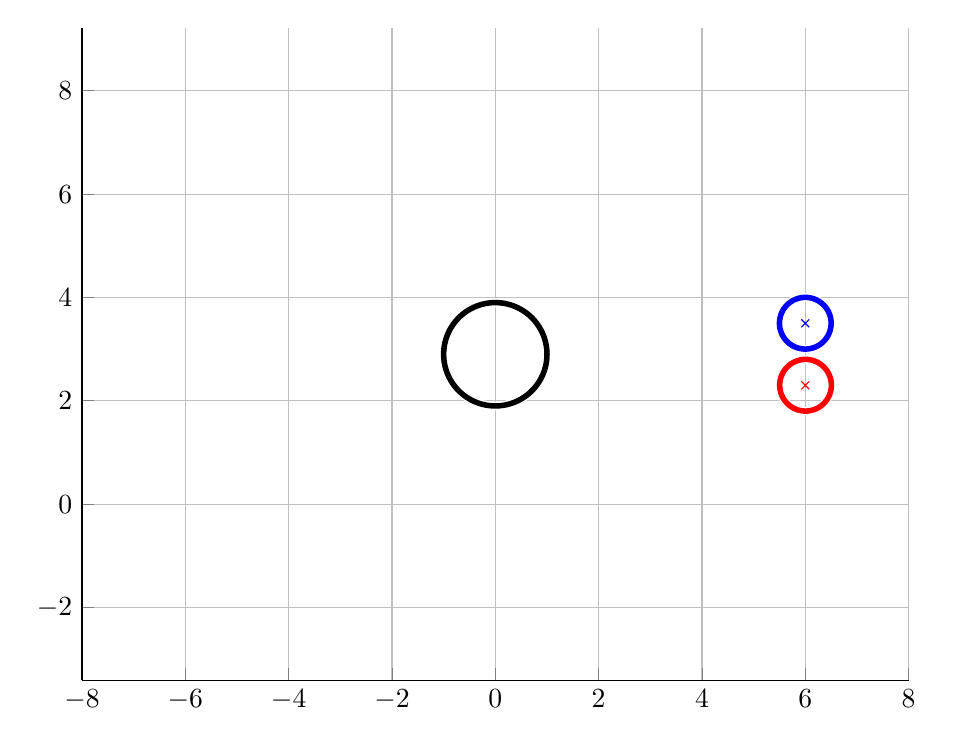
\begin{tikzpicture}

\begin{axis}[%
width=4.133in,
height=3.26in,
at={(0.693in,0.44in)},
scale only axis,
unbounded coords=jump,
xmin=-8,
xmax=8,
xmajorgrids,
ymin=-3.40867808635214,
ymax=9.21067675235754,
ymajorgrids,
axis background/.style={fill=white},
axis x line*=bottom,
axis y line*=left
]
\addplot [color=blue,only marks,mark=x,mark options={solid},forget plot]
  table[row sep=crcr]{%
6	3.5\\
};
\addplot [color=red,only marks,mark=x,mark options={solid},forget plot]
  table[row sep=crcr]{%
6	2.3\\
};
\addplot [color=white,solid,line width=3.0pt,forget plot]
  table[row sep=crcr]{%
6.5000929649555	3.50099998257765\\
6.49978837846504	3.5184497309289\\
6.49887499008541	3.53587821944972\\
6.49735391263963	3.55326421421148\\
6.49522699932628	3.57058653305769\\
6.4924968414616	3.58782407141112\\
6.4891667653224	3.60495582798653\\
6.4852408280935	3.62196093037749\\
6.48072381292466	3.63881866048615\\
6.47562122310307	3.65550847976513\\
6.46993927534845	3.67201005424049\\
6.46368489223889	3.68830327928561\\
6.4568656937768	3.70436830411555\\
6.44948998810508	3.72018555597219\\
6.44156676138496	3.7357357639706\\
6.43310566684772	3.75099998257765\\
6.42411701303371	3.76595961469426\\
6.41461175123302	3.78059643431303\\
6.40460146214297	3.79489260872389\\
6.39409834175886	3.80883072024048\\
6.38311518651499	3.82239378742092\\
6.37166537769419	3.83556528575708\\
6.35976286512482	3.84832916780715\\
6.347422150185	3.86066988274698\\
6.33465826813493	3.87257239531635\\
6.32148676979877	3.88402220413714\\
6.30792370261833	3.89500535938101\\
6.29398559110173	3.90550847976513\\
6.27968941669087	3.91551876885517\\
6.2650525970721	3.92502403065587\\
6.2500929649555	3.93401268446987\\
6.23482874634844	3.94247377900712\\
6.21927853835004	3.95039700572724\\
6.2034612864934	3.95777271139895\\
6.18739626166345	3.96459190986105\\
6.17110303661833	3.97084629297061\\
6.15460146214297	3.97652824072523\\
6.137911642864	3.98163083054681\\
6.12105391275533	3.98614784571565\\
6.10404881036438	3.99007378294456\\
6.08691705378896	3.99340385908376\\
6.06967951543553	3.99613401694844\\
6.05235719658932	3.99826093026179\\
6.03497120182756	3.99978200770757\\
6.01754271330675	4.0006953960872\\
6.0000929649555	4.00099998257765\\
5.98264321660425	4.0006953960872\\
5.96521472808343	3.99978200770757\\
5.94782873332167	3.99826093026179\\
5.93050641447546	3.99613401694844\\
5.91326887612203	3.99340385908376\\
5.89613711954662	3.99007378294456\\
5.87913201715566	3.98614784571565\\
5.862274287047	3.98163083054681\\
5.84558446776802	3.97652824072523\\
5.82908289329266	3.97084629297061\\
5.81278966824754	3.96459190986105\\
5.7967246434176	3.95777271139895\\
5.78090739156096	3.95039700572724\\
5.76535718356255	3.94247377900712\\
5.7500929649555	3.93401268446987\\
5.73513333283889	3.92502403065587\\
5.72049651322012	3.91551876885517\\
5.70620033880926	3.90550847976513\\
5.69226222729267	3.89500535938101\\
5.67869916011223	3.88402220413714\\
5.66552766177607	3.87257239531635\\
5.652763779726	3.86066988274698\\
5.64042306478617	3.84832916780715\\
5.6285205522168	3.83556528575708\\
5.61707074339601	3.82239378742092\\
5.60608758815214	3.80883072024048\\
5.59558446776802	3.79489260872389\\
5.58557417867798	3.78059643431303\\
5.57606891687728	3.76595961469426\\
5.56708026306328	3.75099998257765\\
5.55861916852603	3.7357357639706\\
5.55069594180591	3.72018555597219\\
5.5433202361342	3.70436830411555\\
5.5365010376721	3.68830327928561\\
5.53024665456254	3.67201005424049\\
5.52456470680792	3.65550847976513\\
5.51946211698634	3.63881866048615\\
5.5149451018175	3.62196093037749\\
5.51101916458859	3.60495582798653\\
5.50768908844939	3.58782407141112\\
5.50495893058471	3.57058653305769\\
5.50283201727136	3.55326421421148\\
5.50131093982559	3.53587821944972\\
5.50039755144595	3.5184497309289\\
5.5000929649555	3.50099998257765\\
5.50039755144595	3.4835502342264\\
5.50131093982559	3.46612174570559\\
5.50283201727136	3.44873575094383\\
5.50495893058471	3.43141343209762\\
5.50768908844939	3.41417589374419\\
5.51101916458859	3.39704413716877\\
5.5149451018175	3.38003903477782\\
5.51946211698634	3.36318130466915\\
5.52456470680792	3.34649148539018\\
5.53024665456254	3.32998991091482\\
5.5365010376721	3.3136966858697\\
5.5433202361342	3.29763166103975\\
5.55069594180591	3.28181440918312\\
5.55861916852603	3.26626420118471\\
5.56708026306328	3.25099998257765\\
5.57606891687728	3.23604035046105\\
5.58557417867798	3.22140353084228\\
5.59558446776802	3.20710735643142\\
5.60608758815214	3.19316924491482\\
5.61707074339601	3.17960617773438\\
5.6285205522168	3.16643467939822\\
5.64042306478617	3.15367079734816\\
5.652763779726	3.14133008240833\\
5.66552766177607	3.12942756983896\\
5.67869916011223	3.11797776101816\\
5.69226222729267	3.10699460577429\\
5.70620033880926	3.09649148539018\\
5.72049651322012	3.08648119630013\\
5.73513333283889	3.07697593449944\\
5.7500929649555	3.06798728068543\\
5.76535718356255	3.05952618614819\\
5.78090739156096	3.05160295942807\\
5.7967246434176	3.04422725375635\\
5.81278966824754	3.03740805529426\\
5.82908289329266	3.0311536721847\\
5.84558446776802	3.02547172443008\\
5.862274287047	3.02036913460849\\
5.87913201715566	3.01585211943966\\
5.89613711954662	3.01192618221075\\
5.91326887612203	3.00859610607155\\
5.93050641447546	3.00586594820687\\
5.94782873332167	3.00373903489352\\
5.96521472808343	3.00221795744774\\
5.98264321660425	3.00130456906811\\
6.0000929649555	3.00099998257765\\
6.01754271330675	3.00130456906811\\
6.03497120182756	3.00221795744774\\
6.05235719658932	3.00373903489352\\
6.06967951543553	3.00586594820687\\
6.08691705378896	3.00859610607155\\
6.10404881036438	3.01192618221075\\
6.12105391275533	3.01585211943966\\
6.137911642864	3.02036913460849\\
6.15460146214297	3.02547172443008\\
6.17110303661833	3.0311536721847\\
6.18739626166345	3.03740805529426\\
6.2034612864934	3.04422725375635\\
6.21927853835004	3.05160295942807\\
6.23482874634844	3.05952618614819\\
6.2500929649555	3.06798728068543\\
6.2650525970721	3.07697593449944\\
6.27968941669087	3.08648119630013\\
6.29398559110173	3.09649148539018\\
6.30792370261833	3.10699460577429\\
6.32148676979877	3.11797776101816\\
6.33465826813493	3.12942756983896\\
6.347422150185	3.14133008240833\\
6.35976286512482	3.15367079734816\\
6.37166537769419	3.16643467939822\\
6.38311518651499	3.17960617773438\\
6.39409834175886	3.19316924491482\\
6.40460146214297	3.20710735643142\\
6.41461175123302	3.22140353084228\\
6.42411701303371	3.23604035046105\\
6.43310566684772	3.25099998257765\\
6.44156676138496	3.26626420118471\\
6.44948998810508	3.28181440918312\\
6.4568656937768	3.29763166103975\\
6.46368489223889	3.3136966858697\\
6.46993927534845	3.32998991091482\\
6.47562122310307	3.34649148539018\\
6.48072381292466	3.36318130466915\\
6.4852408280935	3.38003903477782\\
6.4891667653224	3.39704413716877\\
6.4924968414616	3.41417589374419\\
6.49522699932628	3.43141343209762\\
6.49735391263963	3.44873575094383\\
6.49887499008541	3.46612174570559\\
6.49978837846504	3.4835502342264\\
6.5000929649555	3.50099998257765\\
nan	nan\\
};
\addplot [color=blue,solid,line width=2.0pt,forget plot]
  table[row sep=crcr]{%
6.5000929649555	3.50099998257765\\
6.49978837846504	3.5184497309289\\
6.49887499008541	3.53587821944972\\
6.49735391263963	3.55326421421148\\
6.49522699932628	3.57058653305769\\
6.4924968414616	3.58782407141112\\
6.4891667653224	3.60495582798653\\
6.4852408280935	3.62196093037749\\
6.48072381292466	3.63881866048615\\
6.47562122310307	3.65550847976513\\
6.46993927534845	3.67201005424049\\
6.46368489223889	3.68830327928561\\
6.4568656937768	3.70436830411555\\
6.44948998810508	3.72018555597219\\
6.44156676138496	3.7357357639706\\
6.43310566684772	3.75099998257765\\
6.42411701303371	3.76595961469426\\
6.41461175123302	3.78059643431303\\
6.40460146214297	3.79489260872389\\
6.39409834175886	3.80883072024048\\
6.38311518651499	3.82239378742092\\
6.37166537769419	3.83556528575708\\
6.35976286512482	3.84832916780715\\
6.347422150185	3.86066988274698\\
6.33465826813493	3.87257239531635\\
6.32148676979877	3.88402220413714\\
6.30792370261833	3.89500535938101\\
6.29398559110173	3.90550847976513\\
6.27968941669087	3.91551876885517\\
6.2650525970721	3.92502403065587\\
6.2500929649555	3.93401268446987\\
6.23482874634844	3.94247377900712\\
6.21927853835004	3.95039700572724\\
6.2034612864934	3.95777271139895\\
6.18739626166345	3.96459190986105\\
6.17110303661833	3.97084629297061\\
6.15460146214297	3.97652824072523\\
6.137911642864	3.98163083054681\\
6.12105391275533	3.98614784571565\\
6.10404881036438	3.99007378294456\\
6.08691705378896	3.99340385908376\\
6.06967951543553	3.99613401694844\\
6.05235719658932	3.99826093026179\\
6.03497120182756	3.99978200770757\\
6.01754271330675	4.0006953960872\\
6.0000929649555	4.00099998257765\\
5.98264321660425	4.0006953960872\\
5.96521472808343	3.99978200770757\\
5.94782873332167	3.99826093026179\\
5.93050641447546	3.99613401694844\\
5.91326887612203	3.99340385908376\\
5.89613711954662	3.99007378294456\\
5.87913201715566	3.98614784571565\\
5.862274287047	3.98163083054681\\
5.84558446776802	3.97652824072523\\
5.82908289329266	3.97084629297061\\
5.81278966824754	3.96459190986105\\
5.7967246434176	3.95777271139895\\
5.78090739156096	3.95039700572724\\
5.76535718356255	3.94247377900712\\
5.7500929649555	3.93401268446987\\
5.73513333283889	3.92502403065587\\
5.72049651322012	3.91551876885517\\
5.70620033880926	3.90550847976513\\
5.69226222729267	3.89500535938101\\
5.67869916011223	3.88402220413714\\
5.66552766177607	3.87257239531635\\
5.652763779726	3.86066988274698\\
5.64042306478617	3.84832916780715\\
5.6285205522168	3.83556528575708\\
5.61707074339601	3.82239378742092\\
5.60608758815214	3.80883072024048\\
5.59558446776802	3.79489260872389\\
5.58557417867798	3.78059643431303\\
5.57606891687728	3.76595961469426\\
5.56708026306328	3.75099998257765\\
5.55861916852603	3.7357357639706\\
5.55069594180591	3.72018555597219\\
5.5433202361342	3.70436830411555\\
5.5365010376721	3.68830327928561\\
5.53024665456254	3.67201005424049\\
5.52456470680792	3.65550847976513\\
5.51946211698634	3.63881866048615\\
5.5149451018175	3.62196093037749\\
5.51101916458859	3.60495582798653\\
5.50768908844939	3.58782407141112\\
5.50495893058471	3.57058653305769\\
5.50283201727136	3.55326421421148\\
5.50131093982559	3.53587821944972\\
5.50039755144595	3.5184497309289\\
5.5000929649555	3.50099998257765\\
5.50039755144595	3.4835502342264\\
5.50131093982559	3.46612174570559\\
5.50283201727136	3.44873575094383\\
5.50495893058471	3.43141343209762\\
5.50768908844939	3.41417589374419\\
5.51101916458859	3.39704413716877\\
5.5149451018175	3.38003903477782\\
5.51946211698634	3.36318130466915\\
5.52456470680792	3.34649148539018\\
5.53024665456254	3.32998991091482\\
5.5365010376721	3.3136966858697\\
5.5433202361342	3.29763166103975\\
5.55069594180591	3.28181440918312\\
5.55861916852603	3.26626420118471\\
5.56708026306328	3.25099998257765\\
5.57606891687728	3.23604035046105\\
5.58557417867798	3.22140353084228\\
5.59558446776802	3.20710735643142\\
5.60608758815214	3.19316924491482\\
5.61707074339601	3.17960617773438\\
5.6285205522168	3.16643467939822\\
5.64042306478617	3.15367079734816\\
5.652763779726	3.14133008240833\\
5.66552766177607	3.12942756983896\\
5.67869916011223	3.11797776101816\\
5.69226222729267	3.10699460577429\\
5.70620033880926	3.09649148539018\\
5.72049651322012	3.08648119630013\\
5.73513333283889	3.07697593449944\\
5.7500929649555	3.06798728068543\\
5.76535718356255	3.05952618614819\\
5.78090739156096	3.05160295942807\\
5.7967246434176	3.04422725375635\\
5.81278966824754	3.03740805529426\\
5.82908289329266	3.0311536721847\\
5.84558446776802	3.02547172443008\\
5.862274287047	3.02036913460849\\
5.87913201715566	3.01585211943966\\
5.89613711954662	3.01192618221075\\
5.91326887612203	3.00859610607155\\
5.93050641447546	3.00586594820687\\
5.94782873332167	3.00373903489352\\
5.96521472808343	3.00221795744774\\
5.98264321660425	3.00130456906811\\
6.0000929649555	3.00099998257765\\
6.01754271330675	3.00130456906811\\
6.03497120182756	3.00221795744774\\
6.05235719658932	3.00373903489352\\
6.06967951543553	3.00586594820687\\
6.08691705378896	3.00859610607155\\
6.10404881036438	3.01192618221075\\
6.12105391275533	3.01585211943966\\
6.137911642864	3.02036913460849\\
6.15460146214297	3.02547172443008\\
6.17110303661833	3.0311536721847\\
6.18739626166345	3.03740805529426\\
6.2034612864934	3.04422725375635\\
6.21927853835004	3.05160295942807\\
6.23482874634844	3.05952618614819\\
6.2500929649555	3.06798728068543\\
6.2650525970721	3.07697593449944\\
6.27968941669087	3.08648119630013\\
6.29398559110173	3.09649148539018\\
6.30792370261833	3.10699460577429\\
6.32148676979877	3.11797776101816\\
6.33465826813493	3.12942756983896\\
6.347422150185	3.14133008240833\\
6.35976286512482	3.15367079734816\\
6.37166537769419	3.16643467939822\\
6.38311518651499	3.17960617773438\\
6.39409834175886	3.19316924491482\\
6.40460146214297	3.20710735643142\\
6.41461175123302	3.22140353084228\\
6.42411701303371	3.23604035046105\\
6.43310566684772	3.25099998257765\\
6.44156676138496	3.26626420118471\\
6.44948998810508	3.28181440918312\\
6.4568656937768	3.29763166103975\\
6.46368489223889	3.3136966858697\\
6.46993927534845	3.32998991091482\\
6.47562122310307	3.34649148539018\\
6.48072381292466	3.36318130466915\\
6.4852408280935	3.38003903477782\\
6.4891667653224	3.39704413716877\\
6.4924968414616	3.41417589374419\\
6.49522699932628	3.43141343209762\\
6.49735391263963	3.44873575094383\\
6.49887499008541	3.46612174570559\\
6.49978837846504	3.4835502342264\\
6.5000929649555	3.50099998257765\\
nan	nan\\
};
\addplot [color=white,solid,line width=3.0pt,forget plot]
  table[row sep=crcr]{%
6.50467844056058	2.30099868342775\\
6.50437385407013	2.318448431779\\
6.5034604656905	2.33587692029981\\
6.50193938824472	2.35326291506158\\
6.49981247493137	2.37058523390778\\
6.49708231706669	2.38782277226121\\
6.49375224092749	2.40495452883663\\
6.48982630369858	2.42195963122758\\
6.48530928852974	2.43881736133625\\
6.48020669870816	2.45550718061522\\
6.47452475095354	2.47200875509058\\
6.46827036784398	2.48830198013571\\
6.46145116938188	2.50436700496565\\
6.45407546371017	2.52018425682229\\
6.44615223699005	2.53573446482069\\
6.4376911424528	2.55099868342775\\
6.4287024886388	2.56595831554435\\
6.4191972268381	2.58059513516312\\
6.40918693774806	2.59489130957399\\
6.39868381736394	2.60882942109058\\
6.38770066212007	2.62239248827102\\
6.37625085329928	2.63556398660718\\
6.36434834072991	2.64832786865725\\
6.35200762579008	2.66066858359707\\
6.33924374374001	2.67257109616645\\
6.32607224540385	2.68402090498724\\
6.31250917822341	2.69500406023111\\
6.29857106670682	2.70550718061522\\
6.28427489229596	2.71551746970527\\
6.26963807267719	2.72502273150596\\
6.25467844056058	2.73401138531997\\
6.23941422195353	2.74247247985721\\
6.22386401395512	2.75039570657733\\
6.20804676209848	2.75777141224905\\
6.19198173726854	2.76459061071114\\
6.17568851222342	2.7708449938207\\
6.15918693774806	2.77652694157533\\
6.14249711846908	2.78162953139691\\
6.12563938836042	2.78614654656575\\
6.10863428596946	2.79007248379465\\
6.09150252939405	2.79340255993385\\
6.07426499104062	2.79613271779853\\
6.05694267219441	2.79825963111189\\
6.03955667743265	2.79978070855766\\
6.02212818891183	2.8006940969373\\
6.00467844056058	2.80099868342775\\
5.98722869220933	2.8006940969373\\
5.96980020368852	2.79978070855766\\
5.95241420892676	2.79825963111189\\
5.93509189008055	2.79613271779853\\
5.91785435172712	2.79340255993385\\
5.9007225951517	2.79007248379465\\
5.88371749276075	2.78614654656575\\
5.86685976265208	2.78162953139691\\
5.85016994337311	2.77652694157533\\
5.83366836889775	2.7708449938207\\
5.81737514385263	2.76459061071114\\
5.80131011902268	2.75777141224905\\
5.78549286716605	2.75039570657733\\
5.76994265916764	2.74247247985721\\
5.75467844056058	2.73401138531997\\
5.73971880844398	2.72502273150596\\
5.72508198882521	2.71551746970527\\
5.71078581441435	2.70550718061522\\
5.69684770289775	2.69500406023111\\
5.68328463571731	2.68402090498724\\
5.67011313738115	2.67257109616645\\
5.65734925533109	2.66066858359707\\
5.64500854039126	2.64832786865725\\
5.63310602782189	2.63556398660718\\
5.62165621900109	2.62239248827102\\
5.61067306375722	2.60882942109058\\
5.60016994337311	2.59489130957399\\
5.59015965428306	2.58059513516312\\
5.58065439248237	2.56595831554435\\
5.57166573866836	2.55099868342775\\
5.56320464413112	2.53573446482069\\
5.555281417411	2.52018425682229\\
5.54790571173928	2.50436700496565\\
5.54108651327719	2.48830198013571\\
5.53483213016763	2.47200875509058\\
5.52915018241301	2.45550718061522\\
5.52404759259142	2.43881736133625\\
5.51953057742259	2.42195963122758\\
5.51560464019368	2.40495452883663\\
5.51227456405448	2.38782277226121\\
5.5095444061898	2.37058523390778\\
5.50741749287645	2.35326291506158\\
5.50589641543067	2.33587692029981\\
5.50498302705104	2.318448431779\\
5.50467844056058	2.30099868342775\\
5.50498302705104	2.2835489350765\\
5.50589641543067	2.26612044655569\\
5.50741749287645	2.24873445179392\\
5.5095444061898	2.23141213294772\\
5.51227456405448	2.21417459459428\\
5.51560464019368	2.19704283801887\\
5.51953057742259	2.18003773562792\\
5.52404759259142	2.16318000551925\\
5.52915018241301	2.14649018624028\\
5.53483213016763	2.12998861176492\\
5.54108651327719	2.11369538671979\\
5.54790571173928	2.09763036188985\\
5.555281417411	2.08181311003321\\
5.56320464413112	2.0662629020348\\
5.57166573866836	2.05099868342775\\
5.58065439248237	2.03603905131115\\
5.59015965428306	2.02140223169238\\
5.60016994337311	2.00710605728151\\
5.61067306375722	1.99316794576492\\
5.62165621900109	1.97960487858448\\
5.63310602782189	1.96643338024832\\
5.64500854039126	1.95366949819825\\
5.65734925533109	1.94132878325842\\
5.67011313738115	1.92942627068905\\
5.68328463571731	1.91797646186826\\
5.69684770289776	1.90699330662439\\
5.71078581441435	1.89649018624028\\
5.72508198882521	1.88647989715023\\
5.73971880844398	1.87697463534954\\
5.75467844056058	1.86798598153553\\
5.76994265916764	1.85952488699829\\
5.78549286716605	1.85160166027817\\
5.80131011902268	1.84422595460645\\
5.81737514385263	1.83740675614436\\
5.83366836889775	1.8311523730348\\
5.85016994337311	1.82547042528017\\
5.86685976265208	1.82036783545859\\
5.88371749276075	1.81585082028975\\
5.9007225951517	1.81192488306085\\
5.91785435172712	1.80859480692165\\
5.93509189008055	1.80586464905696\\
5.95241420892676	1.80373773574361\\
5.96980020368852	1.80221665829784\\
5.98722869220933	1.8013032699182\\
6.00467844056058	1.80099868342775\\
6.02212818891183	1.8013032699182\\
6.03955667743265	1.80221665829784\\
6.05694267219441	1.80373773574361\\
6.07426499104062	1.80586464905696\\
6.09150252939405	1.80859480692165\\
6.10863428596946	1.81192488306085\\
6.12563938836042	1.81585082028975\\
6.14249711846908	1.82036783545859\\
6.15918693774806	1.82547042528017\\
6.17568851222342	1.8311523730348\\
6.19198173726854	1.83740675614436\\
6.20804676209848	1.84422595460645\\
6.22386401395512	1.85160166027817\\
6.23941422195353	1.85952488699829\\
6.25467844056058	1.86798598153553\\
6.26963807267719	1.87697463534954\\
6.28427489229596	1.88647989715023\\
6.29857106670682	1.89649018624028\\
6.31250917822341	1.90699330662439\\
6.32607224540385	1.91797646186826\\
6.33924374374001	1.92942627068905\\
6.35200762579008	1.94132878325842\\
6.36434834072991	1.95366949819825\\
6.37625085329928	1.96643338024832\\
6.38770066212007	1.97960487858448\\
6.39868381736394	1.99316794576492\\
6.40918693774806	2.00710605728151\\
6.4191972268381	2.02140223169238\\
6.4287024886388	2.03603905131115\\
6.4376911424528	2.05099868342775\\
6.44615223699005	2.0662629020348\\
6.45407546371017	2.08181311003321\\
6.46145116938188	2.09763036188985\\
6.46827036784398	2.11369538671979\\
6.47452475095354	2.12998861176492\\
6.48020669870816	2.14649018624028\\
6.48530928852974	2.16318000551925\\
6.48982630369858	2.18003773562792\\
6.49375224092749	2.19704283801887\\
6.49708231706669	2.21417459459428\\
6.49981247493137	2.23141213294772\\
6.50193938824472	2.24873445179392\\
6.5034604656905	2.26612044655569\\
6.50437385407013	2.2835489350765\\
6.50467844056058	2.30099868342775\\
nan	nan\\
};
\addplot [color=red,solid,line width=2.0pt,forget plot]
  table[row sep=crcr]{%
6.50467844056058	2.30099868342775\\
6.50437385407013	2.318448431779\\
6.5034604656905	2.33587692029981\\
6.50193938824472	2.35326291506158\\
6.49981247493137	2.37058523390778\\
6.49708231706669	2.38782277226121\\
6.49375224092749	2.40495452883663\\
6.48982630369858	2.42195963122758\\
6.48530928852974	2.43881736133625\\
6.48020669870816	2.45550718061522\\
6.47452475095354	2.47200875509058\\
6.46827036784398	2.48830198013571\\
6.46145116938188	2.50436700496565\\
6.45407546371017	2.52018425682229\\
6.44615223699005	2.53573446482069\\
6.4376911424528	2.55099868342775\\
6.4287024886388	2.56595831554435\\
6.4191972268381	2.58059513516312\\
6.40918693774806	2.59489130957399\\
6.39868381736394	2.60882942109058\\
6.38770066212007	2.62239248827102\\
6.37625085329928	2.63556398660718\\
6.36434834072991	2.64832786865725\\
6.35200762579008	2.66066858359707\\
6.33924374374001	2.67257109616645\\
6.32607224540385	2.68402090498724\\
6.31250917822341	2.69500406023111\\
6.29857106670682	2.70550718061522\\
6.28427489229596	2.71551746970527\\
6.26963807267719	2.72502273150596\\
6.25467844056058	2.73401138531997\\
6.23941422195353	2.74247247985721\\
6.22386401395512	2.75039570657733\\
6.20804676209848	2.75777141224905\\
6.19198173726854	2.76459061071114\\
6.17568851222342	2.7708449938207\\
6.15918693774806	2.77652694157533\\
6.14249711846908	2.78162953139691\\
6.12563938836042	2.78614654656575\\
6.10863428596946	2.79007248379465\\
6.09150252939405	2.79340255993385\\
6.07426499104062	2.79613271779853\\
6.05694267219441	2.79825963111189\\
6.03955667743265	2.79978070855766\\
6.02212818891183	2.8006940969373\\
6.00467844056058	2.80099868342775\\
5.98722869220933	2.8006940969373\\
5.96980020368852	2.79978070855766\\
5.95241420892676	2.79825963111189\\
5.93509189008055	2.79613271779853\\
5.91785435172712	2.79340255993385\\
5.9007225951517	2.79007248379465\\
5.88371749276075	2.78614654656575\\
5.86685976265208	2.78162953139691\\
5.85016994337311	2.77652694157533\\
5.83366836889775	2.7708449938207\\
5.81737514385263	2.76459061071114\\
5.80131011902268	2.75777141224905\\
5.78549286716605	2.75039570657733\\
5.76994265916764	2.74247247985721\\
5.75467844056058	2.73401138531997\\
5.73971880844398	2.72502273150596\\
5.72508198882521	2.71551746970527\\
5.71078581441435	2.70550718061522\\
5.69684770289775	2.69500406023111\\
5.68328463571731	2.68402090498724\\
5.67011313738115	2.67257109616645\\
5.65734925533109	2.66066858359707\\
5.64500854039126	2.64832786865725\\
5.63310602782189	2.63556398660718\\
5.62165621900109	2.62239248827102\\
5.61067306375722	2.60882942109058\\
5.60016994337311	2.59489130957399\\
5.59015965428306	2.58059513516312\\
5.58065439248237	2.56595831554435\\
5.57166573866836	2.55099868342775\\
5.56320464413112	2.53573446482069\\
5.555281417411	2.52018425682229\\
5.54790571173928	2.50436700496565\\
5.54108651327719	2.48830198013571\\
5.53483213016763	2.47200875509058\\
5.52915018241301	2.45550718061522\\
5.52404759259142	2.43881736133625\\
5.51953057742259	2.42195963122758\\
5.51560464019368	2.40495452883663\\
5.51227456405448	2.38782277226121\\
5.5095444061898	2.37058523390778\\
5.50741749287645	2.35326291506158\\
5.50589641543067	2.33587692029981\\
5.50498302705104	2.318448431779\\
5.50467844056058	2.30099868342775\\
5.50498302705104	2.2835489350765\\
5.50589641543067	2.26612044655569\\
5.50741749287645	2.24873445179392\\
5.5095444061898	2.23141213294772\\
5.51227456405448	2.21417459459428\\
5.51560464019368	2.19704283801887\\
5.51953057742259	2.18003773562792\\
5.52404759259142	2.16318000551925\\
5.52915018241301	2.14649018624028\\
5.53483213016763	2.12998861176492\\
5.54108651327719	2.11369538671979\\
5.54790571173928	2.09763036188985\\
5.555281417411	2.08181311003321\\
5.56320464413112	2.0662629020348\\
5.57166573866836	2.05099868342775\\
5.58065439248237	2.03603905131115\\
5.59015965428306	2.02140223169238\\
5.60016994337311	2.00710605728151\\
5.61067306375722	1.99316794576492\\
5.62165621900109	1.97960487858448\\
5.63310602782189	1.96643338024832\\
5.64500854039126	1.95366949819825\\
5.65734925533109	1.94132878325842\\
5.67011313738115	1.92942627068905\\
5.68328463571731	1.91797646186826\\
5.69684770289776	1.90699330662439\\
5.71078581441435	1.89649018624028\\
5.72508198882521	1.88647989715023\\
5.73971880844398	1.87697463534954\\
5.75467844056058	1.86798598153553\\
5.76994265916764	1.85952488699829\\
5.78549286716605	1.85160166027817\\
5.80131011902268	1.84422595460645\\
5.81737514385263	1.83740675614436\\
5.83366836889775	1.8311523730348\\
5.85016994337311	1.82547042528017\\
5.86685976265208	1.82036783545859\\
5.88371749276075	1.81585082028975\\
5.9007225951517	1.81192488306085\\
5.91785435172712	1.80859480692165\\
5.93509189008055	1.80586464905696\\
5.95241420892676	1.80373773574361\\
5.96980020368852	1.80221665829784\\
5.98722869220933	1.8013032699182\\
6.00467844056058	1.80099868342775\\
6.02212818891183	1.8013032699182\\
6.03955667743265	1.80221665829784\\
6.05694267219441	1.80373773574361\\
6.07426499104062	1.80586464905696\\
6.09150252939405	1.80859480692165\\
6.10863428596946	1.81192488306085\\
6.12563938836042	1.81585082028975\\
6.14249711846908	1.82036783545859\\
6.15918693774806	1.82547042528017\\
6.17568851222342	1.8311523730348\\
6.19198173726854	1.83740675614436\\
6.20804676209848	1.84422595460645\\
6.22386401395512	1.85160166027817\\
6.23941422195353	1.85952488699829\\
6.25467844056058	1.86798598153553\\
6.26963807267719	1.87697463534954\\
6.28427489229596	1.88647989715023\\
6.29857106670682	1.89649018624028\\
6.31250917822341	1.90699330662439\\
6.32607224540385	1.91797646186826\\
6.33924374374001	1.92942627068905\\
6.35200762579008	1.94132878325842\\
6.36434834072991	1.95366949819825\\
6.37625085329928	1.96643338024832\\
6.38770066212007	1.97960487858448\\
6.39868381736394	1.99316794576492\\
6.40918693774806	2.00710605728151\\
6.4191972268381	2.02140223169238\\
6.4287024886388	2.03603905131115\\
6.4376911424528	2.05099868342775\\
6.44615223699005	2.0662629020348\\
6.45407546371017	2.08181311003321\\
6.46145116938188	2.09763036188985\\
6.46827036784398	2.11369538671979\\
6.47452475095354	2.12998861176492\\
6.48020669870816	2.14649018624028\\
6.48530928852974	2.16318000551925\\
6.48982630369858	2.18003773562792\\
6.49375224092749	2.19704283801887\\
6.49708231706669	2.21417459459428\\
6.49981247493137	2.23141213294772\\
6.50193938824472	2.24873445179392\\
6.5034604656905	2.26612044655569\\
6.50437385407013	2.2835489350765\\
6.50467844056058	2.30099868342775\\
nan	nan\\
};
\addplot [color=white,solid,line width=3.0pt,forget plot]
  table[row sep=crcr]{%
1	2.9\\
0.999390827019096	2.9348994967025\\
0.997564050259824	2.96975647374413\\
0.994521895368273	3.00452846326765\\
0.99026806874157	3.03917310096007\\
0.984807753012208	3.07364817766693\\
0.978147600733806	3.10791169081776\\
0.970295726275996	3.14192189559967\\
0.961261695938319	3.175637355817\\
0.951056516295154	3.20901699437495\\
0.939692620785908	3.24202014332567\\
0.927183854566787	3.27460659341591\\
0.913545457642601	3.3067366430758\\
0.898794046299167	3.33837114678908\\
0.882947592858927	3.36947156278589\\
0.866025403784439	3.4\\
0.848048096156426	3.42991926423321\\
0.829037572555042	3.45919290347075\\
0.809016994374947	3.48778525229247\\
0.788010753606722	3.51566147532566\\
0.766044443118978	3.54278760968654\\
0.743144825477394	3.56913060635886\\
0.719339800338651	3.594658370459\\
0.694658370458997	3.61933980033865\\
0.669130606358858	3.64314482547739\\
0.642787609686539	3.66604444311898\\
0.615661475325658	3.68801075360672\\
0.587785252292473	3.70901699437495\\
0.559192903470747	3.72903757255504\\
0.529919264233205	3.74804809615643\\
0.5	3.76602540378444\\
0.469471562785891	3.78294759285893\\
0.438371146789077	3.79879404629917\\
0.4067366430758	3.8135454576426\\
0.374606593415912	3.82718385456679\\
0.342020143325669	3.83969262078591\\
0.309016994374947	3.85105651629515\\
0.275637355816999	3.86126169593832\\
0.241921895599668	3.870295726276\\
0.207911690817759	3.87814760073381\\
0.17364817766693	3.88480775301221\\
0.139173100960066	3.89026806874157\\
0.104528463267653	3.89452189536827\\
0.0697564737441255	3.89756405025982\\
0.0348994967025011	3.8993908270191\\
6.12323399573677e-17	3.9\\
-0.0348994967025007	3.8993908270191\\
-0.0697564737441253	3.89756405025982\\
-0.104528463267653	3.89452189536827\\
-0.139173100960065	3.89026806874157\\
-0.17364817766693	3.88480775301221\\
-0.207911690817759	3.87814760073381\\
-0.241921895599668	3.870295726276\\
-0.275637355816999	3.86126169593832\\
-0.309016994374947	3.85105651629515\\
-0.342020143325669	3.83969262078591\\
-0.374606593415912	3.82718385456679\\
-0.4067366430758	3.8135454576426\\
-0.438371146789078	3.79879404629917\\
-0.469471562785891	3.78294759285893\\
-0.5	3.76602540378444\\
-0.529919264233205	3.74804809615643\\
-0.559192903470747	3.72903757255504\\
-0.587785252292473	3.70901699437495\\
-0.615661475325658	3.68801075360672\\
-0.642787609686539	3.66604444311898\\
-0.669130606358858	3.64314482547739\\
-0.694658370458997	3.61933980033865\\
-0.719339800338651	3.594658370459\\
-0.743144825477394	3.56913060635886\\
-0.766044443118978	3.54278760968654\\
-0.788010753606722	3.51566147532566\\
-0.809016994374947	3.48778525229247\\
-0.829037572555042	3.45919290347075\\
-0.848048096156426	3.42991926423321\\
-0.866025403784439	3.4\\
-0.882947592858927	3.36947156278589\\
-0.898794046299167	3.33837114678908\\
-0.913545457642601	3.3067366430758\\
-0.927183854566787	3.27460659341591\\
-0.939692620785908	3.24202014332567\\
-0.951056516295154	3.20901699437495\\
-0.961261695938319	3.175637355817\\
-0.970295726275996	3.14192189559967\\
-0.978147600733806	3.10791169081776\\
-0.984807753012208	3.07364817766693\\
-0.99026806874157	3.03917310096007\\
-0.994521895368273	3.00452846326765\\
-0.997564050259824	2.96975647374413\\
-0.999390827019096	2.9348994967025\\
-1	2.9\\
-0.999390827019096	2.8651005032975\\
-0.997564050259824	2.83024352625588\\
-0.994521895368273	2.79547153673235\\
-0.99026806874157	2.76082689903993\\
-0.984807753012208	2.72635182233307\\
-0.978147600733806	2.69208830918224\\
-0.970295726275997	2.65807810440033\\
-0.961261695938319	2.624362644183\\
-0.951056516295154	2.59098300562505\\
-0.939692620785908	2.55797985667433\\
-0.927183854566787	2.52539340658409\\
-0.913545457642601	2.4932633569242\\
-0.898794046299167	2.46162885321092\\
-0.882947592858927	2.43052843721411\\
-0.866025403784439	2.4\\
-0.848048096156426	2.3700807357668\\
-0.829037572555042	2.34080709652925\\
-0.809016994374947	2.31221474770753\\
-0.788010753606722	2.28433852467434\\
-0.766044443118978	2.25721239031346\\
-0.743144825477394	2.23086939364114\\
-0.719339800338651	2.205341629541\\
-0.694658370458997	2.18066019966135\\
-0.669130606358858	2.15685517452261\\
-0.642787609686539	2.13395555688102\\
-0.615661475325658	2.11198924639328\\
-0.587785252292473	2.09098300562505\\
-0.559192903470747	2.07096242744496\\
-0.529919264233205	2.05195190384357\\
-0.5	2.03397459621556\\
-0.469471562785891	2.01705240714107\\
-0.438371146789078	2.00120595370083\\
-0.4067366430758	1.9864545423574\\
-0.374606593415912	1.97281614543321\\
-0.342020143325669	1.96030737921409\\
-0.309016994374948	1.94894348370485\\
-0.275637355816999	1.93873830406168\\
-0.241921895599668	1.929704273724\\
-0.20791169081776	1.92185239926619\\
-0.17364817766693	1.91519224698779\\
-0.139173100960065	1.90973193125843\\
-0.104528463267653	1.90547810463173\\
-0.0697564737441256	1.90243594974018\\
-0.0348994967025016	1.9006091729809\\
-1.83697019872103e-16	1.9\\
0.0348994967025013	1.9006091729809\\
0.0697564737441252	1.90243594974018\\
0.104528463267653	1.90547810463173\\
0.139173100960065	1.90973193125843\\
0.17364817766693	1.91519224698779\\
0.207911690817759	1.92185239926619\\
0.241921895599667	1.929704273724\\
0.275637355816999	1.93873830406168\\
0.309016994374947	1.94894348370485\\
0.342020143325668	1.96030737921409\\
0.374606593415912	1.97281614543321\\
0.406736643075801	1.9864545423574\\
0.438371146789077	2.00120595370083\\
0.46947156278589	2.01705240714107\\
0.5	2.03397459621556\\
0.529919264233205	2.05195190384357\\
0.559192903470746	2.07096242744496\\
0.587785252292473	2.09098300562505\\
0.615661475325659	2.11198924639328\\
0.642787609686539	2.13395555688102\\
0.669130606358858	2.15685517452261\\
0.694658370458997	2.18066019966135\\
0.719339800338651	2.205341629541\\
0.743144825477394	2.23086939364114\\
0.766044443118978	2.25721239031346\\
0.788010753606722	2.28433852467434\\
0.809016994374947	2.31221474770753\\
0.829037572555041	2.34080709652925\\
0.848048096156425	2.37008073576679\\
0.866025403784438	2.4\\
0.882947592858927	2.43052843721411\\
0.898794046299167	2.46162885321092\\
0.913545457642601	2.4932633569242\\
0.927183854566787	2.52539340658409\\
0.939692620785908	2.55797985667433\\
0.951056516295154	2.59098300562505\\
0.961261695938319	2.624362644183\\
0.970295726275996	2.65807810440033\\
0.978147600733806	2.69208830918224\\
0.984807753012208	2.72635182233307\\
0.99026806874157	2.76082689903993\\
0.994521895368273	2.79547153673235\\
0.997564050259824	2.83024352625588\\
0.999390827019096	2.8651005032975\\
1	2.9\\
nan	nan\\
};
\addplot [color=black,solid,line width=2.0pt,forget plot]
  table[row sep=crcr]{%
1	2.9\\
0.999390827019096	2.9348994967025\\
0.997564050259824	2.96975647374413\\
0.994521895368273	3.00452846326765\\
0.99026806874157	3.03917310096007\\
0.984807753012208	3.07364817766693\\
0.978147600733806	3.10791169081776\\
0.970295726275996	3.14192189559967\\
0.961261695938319	3.175637355817\\
0.951056516295154	3.20901699437495\\
0.939692620785908	3.24202014332567\\
0.927183854566787	3.27460659341591\\
0.913545457642601	3.3067366430758\\
0.898794046299167	3.33837114678908\\
0.882947592858927	3.36947156278589\\
0.866025403784439	3.4\\
0.848048096156426	3.42991926423321\\
0.829037572555042	3.45919290347075\\
0.809016994374947	3.48778525229247\\
0.788010753606722	3.51566147532566\\
0.766044443118978	3.54278760968654\\
0.743144825477394	3.56913060635886\\
0.719339800338651	3.594658370459\\
0.694658370458997	3.61933980033865\\
0.669130606358858	3.64314482547739\\
0.642787609686539	3.66604444311898\\
0.615661475325658	3.68801075360672\\
0.587785252292473	3.70901699437495\\
0.559192903470747	3.72903757255504\\
0.529919264233205	3.74804809615643\\
0.5	3.76602540378444\\
0.469471562785891	3.78294759285893\\
0.438371146789077	3.79879404629917\\
0.4067366430758	3.8135454576426\\
0.374606593415912	3.82718385456679\\
0.342020143325669	3.83969262078591\\
0.309016994374947	3.85105651629515\\
0.275637355816999	3.86126169593832\\
0.241921895599668	3.870295726276\\
0.207911690817759	3.87814760073381\\
0.17364817766693	3.88480775301221\\
0.139173100960066	3.89026806874157\\
0.104528463267653	3.89452189536827\\
0.0697564737441255	3.89756405025982\\
0.0348994967025011	3.8993908270191\\
6.12323399573677e-17	3.9\\
-0.0348994967025007	3.8993908270191\\
-0.0697564737441253	3.89756405025982\\
-0.104528463267653	3.89452189536827\\
-0.139173100960065	3.89026806874157\\
-0.17364817766693	3.88480775301221\\
-0.207911690817759	3.87814760073381\\
-0.241921895599668	3.870295726276\\
-0.275637355816999	3.86126169593832\\
-0.309016994374947	3.85105651629515\\
-0.342020143325669	3.83969262078591\\
-0.374606593415912	3.82718385456679\\
-0.4067366430758	3.8135454576426\\
-0.438371146789078	3.79879404629917\\
-0.469471562785891	3.78294759285893\\
-0.5	3.76602540378444\\
-0.529919264233205	3.74804809615643\\
-0.559192903470747	3.72903757255504\\
-0.587785252292473	3.70901699437495\\
-0.615661475325658	3.68801075360672\\
-0.642787609686539	3.66604444311898\\
-0.669130606358858	3.64314482547739\\
-0.694658370458997	3.61933980033865\\
-0.719339800338651	3.594658370459\\
-0.743144825477394	3.56913060635886\\
-0.766044443118978	3.54278760968654\\
-0.788010753606722	3.51566147532566\\
-0.809016994374947	3.48778525229247\\
-0.829037572555042	3.45919290347075\\
-0.848048096156426	3.42991926423321\\
-0.866025403784439	3.4\\
-0.882947592858927	3.36947156278589\\
-0.898794046299167	3.33837114678908\\
-0.913545457642601	3.3067366430758\\
-0.927183854566787	3.27460659341591\\
-0.939692620785908	3.24202014332567\\
-0.951056516295154	3.20901699437495\\
-0.961261695938319	3.175637355817\\
-0.970295726275996	3.14192189559967\\
-0.978147600733806	3.10791169081776\\
-0.984807753012208	3.07364817766693\\
-0.99026806874157	3.03917310096007\\
-0.994521895368273	3.00452846326765\\
-0.997564050259824	2.96975647374413\\
-0.999390827019096	2.9348994967025\\
-1	2.9\\
-0.999390827019096	2.8651005032975\\
-0.997564050259824	2.83024352625588\\
-0.994521895368273	2.79547153673235\\
-0.99026806874157	2.76082689903993\\
-0.984807753012208	2.72635182233307\\
-0.978147600733806	2.69208830918224\\
-0.970295726275997	2.65807810440033\\
-0.961261695938319	2.624362644183\\
-0.951056516295154	2.59098300562505\\
-0.939692620785908	2.55797985667433\\
-0.927183854566787	2.52539340658409\\
-0.913545457642601	2.4932633569242\\
-0.898794046299167	2.46162885321092\\
-0.882947592858927	2.43052843721411\\
-0.866025403784439	2.4\\
-0.848048096156426	2.3700807357668\\
-0.829037572555042	2.34080709652925\\
-0.809016994374947	2.31221474770753\\
-0.788010753606722	2.28433852467434\\
-0.766044443118978	2.25721239031346\\
-0.743144825477394	2.23086939364114\\
-0.719339800338651	2.205341629541\\
-0.694658370458997	2.18066019966135\\
-0.669130606358858	2.15685517452261\\
-0.642787609686539	2.13395555688102\\
-0.615661475325658	2.11198924639328\\
-0.587785252292473	2.09098300562505\\
-0.559192903470747	2.07096242744496\\
-0.529919264233205	2.05195190384357\\
-0.5	2.03397459621556\\
-0.469471562785891	2.01705240714107\\
-0.438371146789078	2.00120595370083\\
-0.4067366430758	1.9864545423574\\
-0.374606593415912	1.97281614543321\\
-0.342020143325669	1.96030737921409\\
-0.309016994374948	1.94894348370485\\
-0.275637355816999	1.93873830406168\\
-0.241921895599668	1.929704273724\\
-0.20791169081776	1.92185239926619\\
-0.17364817766693	1.91519224698779\\
-0.139173100960065	1.90973193125843\\
-0.104528463267653	1.90547810463173\\
-0.0697564737441256	1.90243594974018\\
-0.0348994967025016	1.9006091729809\\
-1.83697019872103e-16	1.9\\
0.0348994967025013	1.9006091729809\\
0.0697564737441252	1.90243594974018\\
0.104528463267653	1.90547810463173\\
0.139173100960065	1.90973193125843\\
0.17364817766693	1.91519224698779\\
0.207911690817759	1.92185239926619\\
0.241921895599667	1.929704273724\\
0.275637355816999	1.93873830406168\\
0.309016994374947	1.94894348370485\\
0.342020143325668	1.96030737921409\\
0.374606593415912	1.97281614543321\\
0.406736643075801	1.9864545423574\\
0.438371146789077	2.00120595370083\\
0.46947156278589	2.01705240714107\\
0.5	2.03397459621556\\
0.529919264233205	2.05195190384357\\
0.559192903470746	2.07096242744496\\
0.587785252292473	2.09098300562505\\
0.615661475325659	2.11198924639328\\
0.642787609686539	2.13395555688102\\
0.669130606358858	2.15685517452261\\
0.694658370458997	2.18066019966135\\
0.719339800338651	2.205341629541\\
0.743144825477394	2.23086939364114\\
0.766044443118978	2.25721239031346\\
0.788010753606722	2.28433852467434\\
0.809016994374947	2.31221474770753\\
0.829037572555041	2.34080709652925\\
0.848048096156425	2.37008073576679\\
0.866025403784438	2.4\\
0.882947592858927	2.43052843721411\\
0.898794046299167	2.46162885321092\\
0.913545457642601	2.4932633569242\\
0.927183854566787	2.52539340658409\\
0.939692620785908	2.55797985667433\\
0.951056516295154	2.59098300562505\\
0.961261695938319	2.624362644183\\
0.970295726275996	2.65807810440033\\
0.978147600733806	2.69208830918224\\
0.984807753012208	2.72635182233307\\
0.99026806874157	2.76082689903993\\
0.994521895368273	2.79547153673235\\
0.997564050259824	2.83024352625588\\
0.999390827019096	2.8651005032975\\
1	2.9\\
nan	nan\\
};
\end{axis}
\end{tikzpicture}%}
      \caption{}
      \label{}
    \end{figure}
  \end{minipage}
\end{minipage}
}

\subsection{State errors}

\noindent\makebox[\linewidth][c]{%
\begin{minipage}{\linewidth}
  \begin{minipage}{0.45\linewidth}
    \begin{figure}[H]
      \scalebox{0.7}{% This file was created by matlab2tikz.
%
%The latest updates can be retrieved from
%  http://www.mathworks.com/matlabcentral/fileexchange/22022-matlab2tikz-matlab2tikz
%where you can also make suggestions and rate matlab2tikz.
%
\definecolor{mycolor1}{rgb}{0.00000,0.44700,0.74100}%
\definecolor{mycolor2}{rgb}{0.85000,0.32500,0.09800}%
\definecolor{mycolor3}{rgb}{0.92900,0.69400,0.12500}%
%
\begin{tikzpicture}

\begin{axis}[%
width=4.133in,
height=3.26in,
at={(0.693in,0.44in)},
scale only axis,
xmin=1,
xmax=100,
xmajorgrids,
ymin=-2,
ymax=2.1,
ymajorgrids,
xlabel={time [iterations]},
ylabel={component magnitude},
axis background/.style={fill=white},
legend style={legend cell align=left,align=left,draw=white!15!black}
]
\addplot [color=mycolor1,solid]
  table[row sep=crcr]{%
1	-12\\
2	-11.0357002192746\\
3	-10.1245109521708\\
4	-9.18738732523736\\
5	-8.23154924519137\\
6	-7.25600583467408\\
7	-6.2631659074083\\
8	-5.25780136980059\\
9	-4.27333244553113\\
10	-3.27763742421729\\
11	-2.29853251285211\\
12	-1.37198786491555\\
13	-0.513946566055827\\
14	0.0866290836164753\\
15	0.33138041035715\\
16	0.278211220698197\\
17	0.118688830590016\\
18	0.00647574150103004\\
19	-0.0187887386409353\\
20	-0.0230860384846833\\
21	-0.0229816026277388\\
22	-0.0220125737276301\\
23	-0.0207292913011952\\
24	-0.0190744192791464\\
25	-0.0169487860226661\\
26	-0.0143111755836636\\
27	-0.0111535158476398\\
28	-0.00754790205743027\\
29	-0.00357592463467942\\
30	0.000622416356660126\\
31	0.00488990857758534\\
32	0.0090349251142785\\
33	0.0128596961588329\\
34	0.0161650305197812\\
35	0.01889382322331\\
36	0.0208567536679179\\
37	0.0219375796994614\\
38	0.0220554135827261\\
39	0.0211936365662433\\
40	0.0193926703104417\\
41	0.0167494567010094\\
42	0.0134104722062194\\
43	0.00949248645968904\\
44	0.00525068288979966\\
45	0.000859582999084783\\
46	-0.00346448609936722\\
47	-0.00753751154861172\\
48	-0.0111798934646757\\
49	-0.0142066685205217\\
50	-0.0165286485024373\\
51	-0.0183531372023017\\
52	-0.0194912850394756\\
53	-0.0199116128350599\\
54	-0.0196282442416332\\
55	-0.0186589490012905\\
56	-0.0170059877359394\\
57	-0.0147147348561698\\
58	-0.011827999830291\\
59	-0.00842174825563343\\
60	-0.00458837382858168\\
61	-0.00045853321938582\\
62	0.00381447036461368\\
63	0.00805035275773843\\
64	0.00260940547172175\\
65	-0.0010425697935171\\
66	0.00331403052141352\\
67	0.0143429171556353\\
68	0.0193439893720467\\
69	0.021457602898198\\
70	0.0217498498904845\\
71	0.0206919815817076\\
72	0.0185609308292246\\
73	0.0155790514150914\\
74	0.0119231608827535\\
75	0.00780552599280427\\
76	0.00345547618620625\\
77	-0.000921581656099039\\
78	-0.00513126751647384\\
79	-0.0089942051275916\\
80	-0.012325501528429\\
81	-0.0149730509867233\\
82	-0.0170513630039659\\
83	-0.018474108853382\\
84	-0.0191999246442107\\
85	-0.0192301116595906\\
86	-0.0185521324775858\\
87	-0.0171808123047706\\
88	-0.0151548791196427\\
89	-0.0125009973310031\\
90	-0.00928881202597453\\
91	-0.00560969043210593\\
92	-0.00156989624882284\\
93	0.00267437991835866\\
94	0.00696751609690567\\
95	-0.00218156594682402\\
96	-0.013323868471841\\
97	-0.0165252589239539\\
98	-0.00325341223677723\\
99	0.0115841437095531\\
100	0.0182144353958477\\
};
\addlegendentry{$\text{e}_{\text{1,1}}$};

\addplot [color=mycolor2,solid]
  table[row sep=crcr]{%
1	0\\
2	0.232537001594962\\
3	0.653275471281589\\
4	1.01945667498219\\
5	1.33945117250341\\
6	1.59848664757482\\
7	1.78426245146688\\
8	1.88166309297038\\
9	1.82649458201547\\
10	1.66845754155366\\
11	1.43764527864374\\
12	1.05249457773444\\
13	0.535389952281192\\
14	0.145657847269637\\
15	0.0348306291766969\\
16	0.0494237401720461\\
17	0.0557030359381731\\
18	0.0503819613603888\\
19	0.0463416831641861\\
20	0.041051999233332\\
21	0.034116320280306\\
22	0.0258175194564708\\
23	0.0165053459903434\\
24	0.00656213106080076\\
25	-0.00360611652788407\\
26	-0.0135849311528754\\
27	-0.0229695438984098\\
28	-0.0313818350926987\\
29	-0.0384873269599104\\
30	-0.0440081632653786\\
31	-0.0477339843523771\\
32	-0.0495291069379937\\
33	-0.0493364544489917\\
34	-0.0471781352666223\\
35	-0.0431512013286606\\
36	-0.0374256230917382\\
37	-0.0302352064829072\\
38	-0.0218685722633768\\
39	-0.0126574065995775\\
40	-0.00296391991424396\\
41	0.0068326142744975\\
42	0.0163494972472264\\
43	0.0252136920915775\\
44	0.0330771153003483\\
45	0.0396266275425059\\
46	0.0445970965967659\\
47	0.0477812248114942\\
48	0.0490386592950794\\
49	0.0483027635395975\\
50	0.0455860464606418\\
51	0.0409855863223959\\
52	0.034673461153531\\
53	0.0268965546175507\\
54	0.0179659830833399\\
55	0.00824344825448849\\
56	-0.00187515498637592\\
57	-0.0119767370166533\\
58	-0.0216502700895608\\
59	-0.0305045360937578\\
60	-0.0381853523506449\\
61	-0.0443899972248424\\
62	-0.0488791705755401\\
63	-0.0514856031421122\\
64	-0.0521709285600031\\
65	-0.0508759175599756\\
66	-0.0475916442887905\\
67	-0.0424043165131101\\
68	-0.0357495462336667\\
69	-0.0278248279246323\\
70	-0.0189230058576981\\
71	-0.00938817138520225\\
72	0.000407961091129701\\
73	0.010083121499107\\
74	0.0192587297701045\\
75	0.0275747567241138\\
76	0.0347022468263333\\
77	0.0403548907754757\\
78	0.0443002709415408\\
79	0.0463694310620696\\
80	0.0464646188549605\\
81	0.044564934256154\\
82	0.0407323440076896\\
83	0.0351078070268537\\
84	0.0279086513983767\\
85	0.01942072446536\\
86	0.00998590185421279\\
87	-1.22126683045102e-05\\
88	-0.0101654783856231\\
89	-0.0200602255875285\\
90	-0.0292949373538215\\
91	-0.03749827907979\\
92	-0.0443448081768035\\
93	-0.0495677211982028\\
94	-0.0529691426309335\\
95	-0.0544777977620498\\
96	-0.0540221801501761\\
97	-0.0516231872946929\\
98	-0.0470406302528498\\
99	-0.0407400444133052\\
100	-0.0332567957636802\\
};
\addlegendentry{$\text{e}_{\text{1,2}}$};

\addplot [color=mycolor3,solid]
  table[row sep=crcr]{%
1	0\\
2	0.472104827277756\\
3	0.390487647064949\\
4	0.349386174381163\\
5	0.288855376623065\\
6	0.219327328026152\\
7	0.136554574904723\\
8	0.0393923258160251\\
9	-0.172830913729049\\
10	-0.16468642388795\\
11	-0.32119317260279\\
12	-0.489441693798394\\
13	-0.615973879791215\\
14	-0.558681773693759\\
15	-0.334368656413803\\
16	-0.0984343812848431\\
17	0.0248035037497457\\
18	0.0425624138646781\\
19	0.00658511771093399\\
20	-0.00716728316980002\\
21	-0.0130072265804752\\
22	-0.0155601477230558\\
23	-0.0163599005346946\\
24	-0.0159835690026965\\
25	-0.0146869451941437\\
26	-0.0126729252601799\\
27	-0.0100847351796093\\
28	-0.00710092457684795\\
29	-0.00389097135358437\\
30	-0.000607118063854719\\
31	0.00259531131753384\\
32	0.00560245868498839\\
33	0.00829012885279613\\
34	0.0105240978562074\\
35	0.0123560775721962\\
36	0.0137198665072179\\
37	0.0146276821487434\\
38	0.0150627345378021\\
39	0.0150145292331992\\
40	0.0144758130191995\\
41	0.0134459732243992\\
42	0.0119456510571471\\
43	0.00995984821292621\\
44	0.00754873279013412\\
45	0.00476087187901179\\
46	0.00168339546464416\\
47	-0.00157473392900512\\
48	-0.00488212792155524\\
49	-0.00806865813958548\\
50	-0.0108547089882912\\
51	-0.0132973680171312\\
52	-0.0151179966331691\\
53	-0.0162471657322007\\
54	-0.0166180817822246\\
55	-0.0161994517321243\\
56	-0.0150310809658162\\
57	-0.0131844989548241\\
58	-0.0107629555282994\\
59	-0.00790084802253239\\
60	-0.00476277654601265\\
61	-0.00149347891174318\\
62	0.00174775672987662\\
63	0.00483831637474835\\
64	0.00520806849598277\\
65	0.00920822264775293\\
66	0.0186663489854961\\
67	0.0183130113106983\\
68	0.0173021002758017\\
69	0.0166396944975856\\
70	0.0160921557345657\\
71	0.0154000425882646\\
72	0.0143957354404437\\
73	0.0129963943598882\\
74	0.0111763519656662\\
75	0.00892271191165527\\
76	0.00628438612477311\\
77	0.00332553054683562\\
78	0.000142506772081861\\
79	-0.00314370990953125\\
80	-0.00638859839292801\\
81	-0.00935772136388043\\
82	-0.0119634774389988\\
83	-0.0140126452097575\\
84	-0.0154219142417219\\
85	-0.0160894984962923\\
86	-0.0159907841058687\\
87	-0.0151241509084665\\
88	-0.0135460241635221\\
89	-0.0113498859956052\\
90	-0.00865306085212153\\
91	-0.00561677919821012\\
92	-0.00239301195103154\\
93	0.000873783112918691\\
94	0.00402388699429119\\
95	0.00182564427600397\\
96	0.00671066141054492\\
97	0.0201170822979769\\
98	0.0330878078344038\\
99	0.0252289816508756\\
100	0.0207268413160135\\
};
\addlegendentry{$\text{e}_{\text{1,3}}$};

\end{axis}
\end{tikzpicture}%
}
      \caption{}
      \label{}
    \end{figure}
  \end{minipage}
  \hfill
  \begin{minipage}{0.45\linewidth}
    \begin{figure}[H]
      \scalebox{0.7}{% This file was created by matlab2tikz.
%
%The latest updates can be retrieved from
%  http://www.mathworks.com/matlabcentral/fileexchange/22022-matlab2tikz-matlab2tikz
%where you can also make suggestions and rate matlab2tikz.
%
\definecolor{mycolor1}{rgb}{0.00000,0.44700,0.74100}%
\definecolor{mycolor2}{rgb}{0.85000,0.32500,0.09800}%
\definecolor{mycolor3}{rgb}{0.92900,0.69400,0.12500}%
%
\begin{tikzpicture}

\begin{axis}[%
width=4.133in,
height=3.26in,
at={(0.693in,0.44in)},
scale only axis,
xmin=1,
xmax=100,
xmajorgrids,
ymin=-2,
ymax=2.5,
ymajorgrids,
axis background/.style={fill=white},
axis x line*=bottom,
axis y line*=left,
legend style={legend cell align=left,align=left,draw=white!15!black}
]
\addplot [color=mycolor1,solid]
  table[row sep=crcr]{%
1	-12\\
2	-11.0025155780855\\
3	-10.0067830149439\\
4	-9.04331062409336\\
5	-8.31314286028116\\
6	-7.57380598224384\\
7	-7.01676427367618\\
8	-6.17128261562075\\
9	-5.22677936426417\\
10	-4.28198674052196\\
11	-3.33338463858648\\
12	-2.38641858405666\\
13	-1.45982580478962\\
14	-0.592901728822402\\
15	-0.175218996521479\\
16	0.0155458180305408\\
17	0.0814492252572294\\
18	0.0730768074857377\\
19	0.027659485553113\\
20	0.00517218303685139\\
21	-0.00625392854934139\\
22	-0.012010832979139\\
23	-0.0150665013042607\\
24	-0.016569558553366\\
25	-0.0170668505298616\\
26	-0.0166988747092271\\
27	-0.0155636108605857\\
28	-0.013762362231661\\
29	-0.0113440287932911\\
30	-0.00838855891675612\\
31	-0.00506405496608146\\
32	-0.00140349019811436\\
33	0.00234673727780162\\
34	0.0061575370735798\\
35	0.00968860209349263\\
36	0.0127204577410364\\
37	0.0152000586066926\\
38	0.0170039243169628\\
39	0.0180457081069549\\
40	0.0182866941589393\\
41	0.0177329116709174\\
42	0.016432582857734\\
43	0.0144441234048131\\
44	0.011910456500658\\
45	0.00896790147674494\\
46	0.00573970057447094\\
47	0.00236862511036366\\
48	-0.000877448085024831\\
49	-0.00414102161354713\\
50	-0.00752372815335668\\
51	-0.0102900761164661\\
52	-0.0127265431409371\\
53	-0.0145118560307464\\
54	-0.0159174152844596\\
55	-0.016826943452654\\
56	-0.0172006882896825\\
57	-0.016920468986705\\
58	-0.0159830661260608\\
59	-0.014418501921126\\
60	-0.0122255823345684\\
61	-0.00946287953743827\\
62	-0.00628634154953279\\
63	-0.00270967901486246\\
64	-0.00270618643174041\\
65	0.0190279513064084\\
66	0.034284757108574\\
67	0.0231655190963145\\
68	0.0195585701191076\\
69	0.0188371190381029\\
70	0.0189705006463705\\
71	0.019011092332268\\
72	0.0185526811829833\\
73	0.0174531297041144\\
74	0.0157068395467299\\
75	0.0133635592782063\\
76	0.010559665678478\\
77	0.00741799955660272\\
78	0.00407006799452955\\
79	0.000663824032288402\\
80	-0.00257520704466269\\
81	-0.00581350739861375\\
82	-0.00881762267275386\\
83	-0.0114924967744732\\
84	-0.0137600017465637\\
85	-0.0152698175088686\\
86	-0.0163713485502493\\
87	-0.0169960841730451\\
88	-0.0169630762486363\\
89	-0.0162946729674243\\
90	-0.0149927017414689\\
91	-0.0130467823234011\\
92	-0.010500710480397\\
93	-0.00743372392797708\\
94	-0.00400715122715268\\
95	-0.00405266004954686\\
96	0.0238158193519805\\
97	0.0546505946655873\\
98	0.0362596738032701\\
99	0.024782285086816\\
100	0.0208621808926534\\
};
\addlegendentry{$\text{e}_\text{1}$};

\addplot [color=mycolor2,solid]
  table[row sep=crcr]{%
1	0\\
2	0.0734493405915497\\
3	0.195383281647995\\
4	0.46573015758082\\
5	0.705112833886585\\
6	1.0673623498366\\
7	1.7230130897688\\
8	2.20403885464816\\
9	2.0557815100345\\
10	1.71078923470268\\
11	1.37696513179543\\
12	1.04016344255604\\
13	0.65403116762763\\
14	0.267401732547045\\
15	0.109245235997813\\
16	0.0596921376689867\\
17	0.0494812011685947\\
18	0.0483960983040716\\
19	0.0460519488598485\\
20	0.0410881506742685\\
21	0.0343002552335189\\
22	0.0260885188845493\\
23	0.0168295191652619\\
24	0.00691403862005501\\
25	-0.00324650009057758\\
26	-0.0132361064310308\\
27	-0.0226467216831958\\
28	-0.0310958676303905\\
29	-0.0382441109283438\\
30	-0.0438080485118995\\
31	-0.0475723194433145\\
32	-0.0493967886613313\\
33	-0.04922016703472\\
34	-0.0470627364050644\\
35	-0.0430256259081372\\
36	-0.0372832114445414\\
37	-0.030072829215219\\
38	-0.0216878465859082\\
39	-0.0124644707199715\\
40	-0.0027683764022702\\
41	0.00701916398813573\\
42	0.0165152756459844\\
43	0.0253486793397487\\
44	0.033174188444298\\
45	0.0396833344773872\\
46	0.0446153562404934\\
47	0.0477675121028986\\
48	0.0490033780035441\\
49	0.0482588054259644\\
50	0.0455497843782094\\
51	0.0409646616013608\\
52	0.0346758271726263\\
53	0.026921989560198\\
54	0.0180139071291142\\
55	0.00830705448788835\\
56	-0.00180634326925798\\
57	-0.0119171497646936\\
58	-0.0216139437749607\\
59	-0.0305028921607426\\
60	-0.0382261187861672\\
61	-0.0444756362916693\\
62	-0.0490071142357973\\
63	-0.0516485289774798\\
64	-0.0523030194782968\\
65	-0.0503765121465703\\
66	-0.0467874073713813\\
67	-0.0419723950597396\\
68	-0.0354375716039633\\
69	-0.0275481242340815\\
70	-0.0186516222440958\\
71	-0.00911662340741814\\
72	0.000674097638470058\\
73	0.0103338480089214\\
74	0.0194840147147401\\
75	0.0277662279663165\\
76	0.0348553419387259\\
77	0.0404694381909897\\
78	0.0443806529143333\\
79	0.0464241523578531\\
80	0.0465051675954086\\
81	0.0446053422919864\\
82	0.0407846552638454\\
83	0.0351811105285506\\
84	0.0280073154891398\\
85	0.0195393341166263\\
86	0.0101208336539157\\
87	0.000130699422856801\\
88	-0.0100286293645188\\
89	-0.0199432769564974\\
90	-0.0292103626702026\\
91	-0.0374555908867751\\
92	-0.0443484891211955\\
93	-0.0496166415633784\\
94	-0.0530572403985589\\
95	-0.0545259430485439\\
96	-0.053064874298164\\
97	-0.0496329339102015\\
98	-0.0456639576535213\\
99	-0.0397827411468923\\
100	-0.032418406827508\\
};
\addlegendentry{$\text{e}_\text{2}$};

\addplot [color=mycolor3,solid]
  table[row sep=crcr]{%
1	0\\
2	0.145492094313047\\
3	0.0933855810949526\\
4	0.447365369518162\\
5	0.175691844587656\\
6	0.726878981486458\\
7	1.00874555658001\\
8	0.018365087158827\\
9	-0.353755180859761\\
10	-0.371896082187484\\
11	-0.329062813452435\\
12	-0.376545771026098\\
13	-0.432827723317859\\
14	-0.423125403671976\\
15	-0.325883694870049\\
16	-0.212535212119303\\
17	-0.109511318447447\\
18	-0.0346572688615711\\
19	-0.0208871052155876\\
20	-0.0172721000561035\\
21	-0.0173130614031795\\
22	-0.0181916114365638\\
23	-0.0189125755430272\\
24	-0.019056220496669\\
25	-0.0184675665590513\\
26	-0.0171276735828986\\
27	-0.0150988413384514\\
28	-0.0124763711093395\\
29	-0.00939482655476086\\
30	-0.00600285938715657\\
31	-0.00268135836751927\\
32	0.00086294627583336\\
33	0.00436213098929583\\
34	0.00776474841744381\\
35	0.0107286814121144\\
36	0.0131280400860346\\
37	0.0150953824223149\\
38	0.0165493753197204\\
39	0.017446105674404\\
40	0.0177473716272179\\
41	0.0174270197693528\\
42	0.0164735879029829\\
43	0.014900593114318\\
44	0.0127043354393308\\
45	0.00995091228057111\\
46	0.00673256581837178\\
47	0.00317393605875815\\
48	-0.000561243329616692\\
49	-0.00429609478936252\\
50	-0.00814480676289307\\
51	-0.0114531592718063\\
52	-0.0143273544080035\\
53	-0.0164234176816058\\
54	-0.0178331534679063\\
55	-0.0184687757896019\\
56	-0.0182834435665139\\
57	-0.0173025359105412\\
58	-0.0155709143441468\\
59	-0.0131875094808596\\
60	-0.0102862286983344\\
61	-0.00701266846563071\\
62	-0.00377674218664663\\
63	-0.000247751646181056\\
64	0.0234864210446452\\
65	0.0352866126409965\\
66	0.0183734745654194\\
67	0.0144006728055928\\
68	0.0149405351678634\\
69	0.0161283531892577\\
70	0.017216291557199\\
71	0.0178121419984086\\
72	0.0177937009995102\\
73	0.0171289719087627\\
74	0.0158212255863991\\
75	0.0138813940874819\\
76	0.0113659861268496\\
77	0.00834103592488018\\
78	0.00492096386409153\\
79	0.00124099365871119\\
80	-0.00248767270536675\\
81	-0.00621360313807954\\
82	-0.00973751304939458\\
83	-0.0128544002845235\\
84	-0.0154024224198051\\
85	-0.017053359913468\\
86	-0.0179901176565013\\
87	-0.018127292379558\\
88	-0.0174595032838833\\
89	-0.016021720020405\\
90	-0.0138925655376046\\
91	-0.0111912109422883\\
92	-0.0080576784988853\\
93	-0.00464329945627855\\
94	-0.00132451676197667\\
95	0.027734906652175\\
96	0.0425620714284822\\
97	0.0252742255008026\\
98	0.00822122237916307\\
99	0.0107726451511536\\
100	0.0137609742308591\\
};
\addlegendentry{$\text{e}_\text{3}$};

\end{axis}
\end{tikzpicture}%}
      \caption{}
      \label{}
    \end{figure}
  \end{minipage}
\end{minipage}
}


\subsection{Distances between actors}

\noindent\makebox[\linewidth][c]{%
\begin{minipage}{\linewidth}
  \begin{minipage}{0.45\linewidth}
    \begin{figure}[H]
      \scalebox{0.7}{% This file was created by matlab2tikz.
%
%The latest updates can be retrieved from
%  http://www.mathworks.com/matlabcentral/fileexchange/22022-matlab2tikz-matlab2tikz
%where you can also make suggestions and rate matlab2tikz.
%
\definecolor{mycolor1}{rgb}{0.00000,1.00000,1.00000}%
\definecolor{mycolor2}{rgb}{0.00000,0.44700,0.74100}%

%
\begin{tikzpicture}

\begin{axis}[%
width=4.133in,
height=3.26in,
at={(0.693in,0.44in)},
scale only axis,
xmin=0,
xmax=100,
xmajorgrids,
ymin=0.8,
ymax=2.2,
ymajorgrids,
xlabel={time [iterations]},
ylabel={distance},
axis background/.style={fill=white},
axis x line*=bottom,
axis y line*=left,
legend style={at={(0.705,0.603)},anchor=south west,legend cell align=left,align=left,draw=white!15!black}
]
\addplot [color=mycolor1,solid]
  table[row sep=crcr]{%
0	1.01\\
100	1.01\\
};
\addlegendentry{$\text{d}_{\text{max}}$};

\addplot [color=mycolor1,solid]
  table[row sep=crcr]{%
0	2.01\\
100 2.01\\
};
\addlegendentry{$\text{d}_{\text{min}}$};

\addplot [color=mycolor2,solid]
  table[row sep=crcr]{%
1	1.2\\
2	1.195453701381\\
3	1.19221192721025\\
4	1.03810756595803\\
5	1.04448115109855\\
6	1.04860844573022\\
7	1.04889330055182\\
8	1.11958682710872\\
9	1.03301585242218\\
10	1.03935080847165\\
11	1.08472869139608\\
12	1.13196112931488\\
13	1.13155173557831\\
14	1.08903404565209\\
15	1.16212682905938\\
16	1.19534819193989\\
17	1.20319259605862\\
18	1.2029845584422\\
19	1.20106589559527\\
20	1.20057269403302\\
21	1.20047640096017\\
22	1.20045610763432\\
23	1.2004484214441\\
24	1.20044464075202\\
25	1.20044289496236\\
26	1.2004410179759\\
27	1.20044012822907\\
28	1.20043956023646\\
29	1.20043901439351\\
30	1.20043850879976\\
31	1.20043808253415\\
32	1.20043774699236\\
33	1.20043752481135\\
34	1.20043741442348\\
35	1.20043742020455\\
36	1.20043753578315\\
37	1.20043774827459\\
38	1.2004380410435\\
39	1.20043839653683\\
40	1.20043879842572\\
41	1.2004392318364\\
42	1.20043968166116\\
43	1.20044015395988\\
44	1.20044072074194\\
45	1.20044112938784\\
46	1.20044153693091\\
47	1.20044185691314\\
48	1.20044207818681\\
49	1.20044219699199\\
50	1.20044221542051\\
51	1.200442088671\\
52	1.2004418360631\\
53	1.20044144224355\\
54	1.2004409546646\\
55	1.20044037519516\\
56	1.20043996311818\\
57	1.20044008430599\\
58	1.20043886783678\\
59	1.20043773461665\\
60	1.20043693012392\\
61	1.2004362946554\\
62	1.20043579151607\\
63	1.20043539651881\\
64	1.20039878782014\\
65	1.20026965993915\\
66	1.20020666397755\\
67	1.20024536192205\\
68	1.20026863570747\\
69	1.2002815786186\\
70	1.20028725680473\\
71	1.20028959928224\\
72	1.20029060505626\\
73	1.20029113520667\\
74	1.2002915065904\\
75	1.20029184699655\\
76	1.20029212413476\\
77	1.20029239446525\\
78	1.20029262216883\\
79	1.2002927961451\\
80	1.20029290153441\\
81	1.20029293732429\\
82	1.20029289181258\\
83	1.20029276322213\\
84	1.20029255127225\\
85	1.2002922480852\\
86	1.20029188523799\\
87	1.20029161966177\\
88	1.20029112110291\\
89	1.20029072540458\\
90	1.20029025884671\\
91	1.20028981381966\\
92	1.20028940731404\\
93	1.20028905154728\\
94	1.20028876318802\\
95	1.2002325780391\\
96	1.20022497292368\\
97	1.20040476080958\\
98	1.20020949981807\\
99	1.20013272780385\\
100	1.20011361094771\\
};
\addlegendentry{$\text{d}_{\text{12,a}}$};

\end{axis}
\end{tikzpicture}%
}
      \caption{}
      \label{}
    \end{figure}
  \end{minipage}
  \hfill
  \begin{minipage}{0.45\linewidth}
    \begin{figure}[H]
      \scalebox{0.7}{% This file was created by matlab2tikz.
%
%The latest updates can be retrieved from
%  http://www.mathworks.com/matlabcentral/fileexchange/22022-matlab2tikz-matlab2tikz
%where you can also make suggestions and rate matlab2tikz.
%
\definecolor{mycolor1}{rgb}{0.00000,0.44700,0.74100}%
\definecolor{mycolor2}{rgb}{0.85000,0.32500,0.09800}%
%
\begin{tikzpicture}

\begin{axis}[%
width=4.133in,
height=3.26in,
at={(0.693in,0.44in)},
scale only axis,
xmin=1,
xmax=30,
xmajorgrids,
ymin=1,
ymax=6.5,
ymajorgrids,
axis background/.style={fill=white}
]
\addplot [color=mycolor1,solid,forget plot]
  table[row sep=crcr]{%
1	6.02992537267253\\
2	5.04046321855403\\
3	4.06035423743759\\
4	3.11388249889649\\
5	2.27207498093866\\
6	1.7018536906832\\
7	1.6\\
8	1.82019643698784\\
9	2.27754404279172\\
10	3.01603291996687\\
11	3.84159714379788\\
12	4.71453423398159\\
13	5.53902258565842\\
14	5.85598882707424\\
15	5.97210583637757\\
16	6.01231203824224\\
17	6.02525564178097\\
18	6.02902596351309\\
19	6.0299460861786\\
20	6.03011745882008\\
21	6.03011188288531\\
22	6.03008826615685\\
23	6.03006086183827\\
24	6.03002916739369\\
25	6.03004468508774\\
26	6.03005429435796\\
27	6.03005428435231\\
28	6.03003993648414\\
29	6.03001632652362\\
30	6.02999420433031\\
};
\addplot [color=mycolor2,solid,forget plot]
  table[row sep=crcr]{%
1	6.02992537267253\\
2	5.03148302473864\\
3	4.03178130665471\\
4	3.03221385560332\\
5	2.05551024119015\\
6	1.62554715142378\\
7	1.6\\
8	1.66210954473871\\
9	1.60891897271201\\
10	1.94787944401614\\
11	2.65458136663876\\
12	3.49695460848774\\
13	4.39598594857884\\
14	5.3311251823429\\
15	5.82007164848119\\
16	5.99515265377714\\
17	6.04081644951535\\
18	6.04445966667995\\
19	6.03917726706026\\
20	6.03448139874409\\
21	6.0318390491008\\
22	6.03065825207128\\
23	6.03023506163262\\
24	6.0300372748768\\
25	6.02992615766076\\
26	6.02984177338413\\
27	6.0297991218319\\
28	6.02975309526427\\
29	6.02972907062529\\
30	6.02970391694226\\
};
\end{axis}
\end{tikzpicture}%}
      \caption{}
      \label{}
    \end{figure}
  \end{minipage}
\end{minipage}
}


\subsection{Input signals}

\noindent\makebox[\linewidth][c]{%
\begin{minipage}{\linewidth}
  \begin{minipage}{0.45\linewidth}
    \begin{figure}[H]
      \scalebox{0.7}{% This file was created by matlab2tikz.
%
%The latest updates can be retrieved from
%  http://www.mathworks.com/matlabcentral/fileexchange/22022-matlab2tikz-matlab2tikz
%where you can also make suggestions and rate matlab2tikz.
%
\definecolor{mycolor1}{rgb}{0.00000,1.00000,1.00000}%
\definecolor{mycolor2}{rgb}{0.00000,0.44700,0.74100}%
\definecolor{mycolor3}{rgb}{0.85000,0.32500,0.09800}%
%
\begin{tikzpicture}

\begin{axis}[%
width=4.133in,
height=3.26in,
at={(0.693in,0.44in)},
scale only axis,
xmin=0,
xmax=100,
xmajorgrids,
ymin=-11,
ymax=11,
ymajorgrids,
xlabel={time [iterations]},
ylabel={component magnitude},
axis background/.style={fill=white},
axis x line*=bottom,
axis y line*=left,
legend style={at={(0.697,0.634)},anchor=south west,legend cell align=left,align=left,draw=white!15!black}
]
\addplot [color=mycolor1,solid]
  table[row sep=crcr]{%
0	-10\\
100 -10\\
};
\addlegendentry{$\text{u}_{\text{max}}$};

\addplot [color=mycolor1,solid]
  table[row sep=crcr]{%
0	10\\
100 10\\
};
\addlegendentry{$\text{u}_{\text{min}}$};

\addplot [color=mycolor2,solid]
  table[row sep=crcr]{%
1	10\\
2	10\\
3	10\\
4	10\\
5	10\\
6	10\\
7	9.88563464881492\\
8	8.617970781367\\
9	9.43082904695664\\
10	9.54579411653452\\
11	9.54828897347126\\
12	8.0369360565408\\
13	3.59236261948567\\
14	1.67874054758745\\
15	0.880325536676882\\
16	0.306328944755582\\
17	-0.179253512608004\\
18	-0.441319071247606\\
19	-0.128029813103025\\
20	-0.00724727723974293\\
21	0.0461908711891062\\
22	0.0734095407652387\\
23	0.0890554575775679\\
24	0.0979190153221654\\
25	0.103692379881643\\
26	0.104542574783857\\
27	0.101348279853206\\
28	0.0947156723739461\\
29	0.0845584531071563\\
30	0.0705583055350402\\
31	0.0547710156800228\\
32	0.0358025927754855\\
33	0.0166102894699661\\
34	-0.00513278904702978\\
35	-0.0274586667939475\\
36	-0.0480076549272814\\
37	-0.0668912520582338\\
38	-0.0832537058678003\\
39	-0.0962688787733947\\
40	-0.105288610927618\\
41	-0.109847998214286\\
42	-0.109959000386839\\
43	-0.105007808826879\\
44	-0.0956690053233345\\
45	-0.0822783136338863\\
46	-0.0655427622956162\\
47	-0.0448516662360305\\
48	-0.0251013549133526\\
49	-0.00666959620988991\\
50	0.0180445394212661\\
51	0.0380701236391535\\
52	0.0588245929074031\\
53	0.0737991685561259\\
54	0.0864438232025384\\
55	0.095547055959881\\
56	0.101684333140799\\
57	0.104875885355708\\
58	0.103219147980359\\
59	0.0980637276995874\\
60	0.0893519695847831\\
61	0.0766384456922198\\
62	0.0620243710572437\\
63	-0.0414867896360675\\
64	0.162024981749064\\
65	0.0749688258949881\\
66	-0.0841920158708048\\
67	-0.0704098698822007\\
68	-0.0733352514711834\\
69	-0.0830723063277927\\
70	-0.0940379046377687\\
71	-0.103229872877285\\
72	-0.109022377267241\\
73	-0.110583525346555\\
74	-0.107759513696461\\
75	-0.100177721778053\\
76	-0.0884093059061953\\
77	-0.0730619343328041\\
78	-0.0546514377924147\\
79	-0.0331605222433453\\
80	-0.01330758832124\\
81	0.0081241026591478\\
82	0.0289847879361911\\
83	0.0484083752578333\\
84	0.0685042003605891\\
85	0.0817704056866515\\
86	0.0919394999616318\\
87	0.100205860452808\\
88	0.104089071134004\\
89	0.104155350409535\\
90	0.100650902150989\\
91	0.0934759701181015\\
92	0.0828023610761555\\
93	0.0684359690155335\\
94	-0.0393461403539833\\
95	0.26396831867213\\
96	0.309463171063702\\
97	-0.248745135657556\\
98	-0.13956371912648\\
99	-0.100250002879208\\
100	-0.0914249701536794\\
};
\addlegendentry{$\text{u}_{\text{1,1}}$};

\addplot [color=mycolor3,solid]
  table[row sep=crcr]{%
1	1.35357466319134\\
2	-0.433213081726238\\
3	0.256710915459715\\
4	1.40903609044249\\
5	-0.318919108777255\\
6	-2.03259334540993\\
7	-3.02668224280666\\
8	1.58360387417738\\
9	-0.619486850972193\\
10	-0.885312441796456\\
11	-0.352290100704846\\
12	0.103402732315297\\
13	0.255374885148664\\
14	0.237546117651611\\
15	0.414513849397488\\
16	0.634582333299252\\
17	0.593870846212467\\
18	0.0724150879644183\\
19	-0.138971911325582\\
20	-0.0304566265359456\\
21	0.0294277159203628\\
22	0.0653070555995963\\
23	0.0879556895594226\\
24	0.102018439021225\\
25	0.109838746636651\\
26	0.111946914701224\\
27	0.108985324902349\\
28	0.101104432733423\\
29	0.0888351837438188\\
30	0.0705275538203381\\
31	0.0536330062168194\\
32	0.033330203623393\\
33	0.0125706770591512\\
34	-0.0107550979122996\\
35	-0.03372488475196\\
36	-0.053074138459\\
37	-0.0703356798245091\\
38	-0.084653732183112\\
39	-0.0956213274197397\\
40	-0.102917876962661\\
41	-0.106352698204285\\
42	-0.105823892157001\\
43	-0.10174482872188\\
44	-0.0936941695451027\\
45	-0.0821922111327252\\
46	-0.0674510130965137\\
47	-0.0497966923328603\\
48	-0.0298656834316683\\
49	-0.0113742736779633\\
50	0.0125696160897144\\
51	0.0336362131665264\\
52	0.0556565852563023\\
53	0.0737070138401524\\
54	0.0891372984770748\\
55	0.101211411406675\\
56	0.109152152462715\\
57	0.112207760863548\\
58	0.11139605950152\\
59	0.105153875572186\\
60	0.0944801057829419\\
61	0.0772774388314807\\
62	0.0615909451714991\\
63	0.203232849451359\\
64	0.149754836048525\\
65	-0.170417671035434\\
66	-0.101269474584421\\
67	-0.0738150309931737\\
68	-0.0739435135376231\\
69	-0.0828161643953188\\
70	-0.0928175102181253\\
71	-0.100824195813705\\
72	-0.105583879000294\\
73	-0.106610905014541\\
74	-0.103943439176237\\
75	-0.0973673041828961\\
76	-0.0872989688581445\\
77	-0.0738273287122778\\
78	-0.0574289432223596\\
79	-0.038098819633525\\
80	-0.0182190736740477\\
81	0.00288712828891981\\
82	0.0245283478037947\\
83	0.0455647423594786\\
84	0.0670506713465768\\
85	0.0833809420292917\\
86	0.0968454120526324\\
87	0.106548647626267\\
88	0.111747206009294\\
89	0.112375164191684\\
90	0.108185577079603\\
91	0.099352632857835\\
92	0.0862928561859735\\
93	0.0673913812266591\\
94	0.297330164283001\\
95	0.177058455818324\\
96	-0.180888814372683\\
97	-0.162444381595988\\
98	-0.0818837966770668\\
99	-0.0701797042052921\\
100	-0.0759990736352368\\
};
\addlegendentry{$\text{u}_{\text{1,2}}$};

\end{axis}
\end{tikzpicture}%
}
      \caption{}
      \label{}
    \end{figure}
  \end{minipage}
  \hfill
  \begin{minipage}{0.45\linewidth}
    \begin{figure}[H]
      \scalebox{0.7}{% This file was created by matlab2tikz.
%
%The latest updates can be retrieved from
%  http://www.mathworks.com/matlabcentral/fileexchange/22022-matlab2tikz-matlab2tikz
%where you can also make suggestions and rate matlab2tikz.
%
\definecolor{mycolor1}{rgb}{0.00000,1.00000,1.00000}%
\definecolor{mycolor2}{rgb}{0.00000,0.44700,0.74100}%
\definecolor{mycolor3}{rgb}{0.85000,0.32500,0.09800}%
%
\begin{tikzpicture}

\begin{axis}[%
width=4.133in,
height=3.26in,
at={(0.693in,0.44in)},
scale only axis,
xmin=0,
xmax=100,
xmajorgrids,
ymin=-11,
ymax=11,
ymajorgrids,
xlabel={time [iterations]},
axis background/.style={fill=white},
axis x line*=bottom,
axis y line*=left,
legend style={at={(0.711,0.647)},anchor=south west,legend cell align=left,align=left,draw=white!15!black}
]
\addplot [color=mycolor1,solid]
  table[row sep=crcr]{%
0	-10\\
100 -10\\
};
\addlegendentry{$\text{u}_{\text{max}}$};

\addplot [color=mycolor1,solid]
  table[row sep=crcr]{%
0	10\\
100 10\\
};
\addlegendentry{$\text{u}_{\text{min}}$};

\addplot [color=mycolor2,solid]
  table[row sep=crcr]{%
1	10\\
2	10\\
3	10\\
4	7.62646030689056\\
5	8.23238925448627\\
6	8.50605849114632\\
7	10\\
8	9.53333796017539\\
9	10\\
10	10\\
11	10\\
12	10\\
13	9.46244587339416\\
14	4.44353093140653\\
15	1.95510798940484\\
16	0.663741277055059\\
17	-0.0681679806667713\\
18	-0.419316530160271\\
19	-0.172008612377067\\
20	-0.0456057940803135\\
21	0.0241261169104589\\
22	0.0609177015519929\\
23	0.0825744239213155\\
24	0.0948695300477512\\
25	0.101777541925431\\
26	0.103793478616532\\
27	0.101110356939594\\
28	0.0946256538353053\\
29	0.0845341550957334\\
30	0.0705711703526584\\
31	0.0547916132093406\\
32	0.0358238111744648\\
33	0.0166321321956878\\
34	-0.0051071136914514\\
35	-0.0274309754883406\\
36	-0.0479841699370514\\
37	-0.0668716203481734\\
38	-0.0832378503186649\\
39	-0.0962572100630007\\
40	-0.105281848598472\\
41	-0.109846561213383\\
42	-0.109965156679194\\
43	-0.105062540105777\\
44	-0.095618334186855\\
45	-0.0823036318493377\\
46	-0.0655683255323942\\
47	-0.0448855170720054\\
48	-0.0251332211808633\\
49	-0.00669640067377911\\
50	0.0180147390973399\\
51	0.0380413784780437\\
52	0.0587944326067577\\
53	0.0737781693643875\\
54	0.086423021973116\\
55	0.0956564763176469\\
56	0.10210797431113\\
57	0.104631262412459\\
58	0.103055821488982\\
59	0.0980075298320563\\
60	0.0893412516083411\\
61	0.0766564339085556\\
62	0.0620461332449234\\
63	0.00665666027544988\\
64	0.204128698180137\\
65	0.119919249419318\\
66	-0.161995270144651\\
67	-0.102925818290311\\
68	-0.0874694812842944\\
69	-0.0891230274541853\\
70	-0.0966476711980842\\
71	-0.10436510907873\\
72	-0.109525081656196\\
73	-0.110811823530772\\
74	-0.107878654828526\\
75	-0.100214808489331\\
76	-0.0884456436560771\\
77	-0.0730890000820963\\
78	-0.0546751124117797\\
79	-0.033185325392665\\
80	-0.0133290638620536\\
81	0.00810259430906069\\
82	0.0289653387213678\\
83	0.0483896760097334\\
84	0.0684854906916422\\
85	0.081754778792505\\
86	0.0920101689951137\\
87	0.100156839360677\\
88	0.104098769343487\\
89	0.104137710503525\\
90	0.100647516051874\\
91	0.0934830777068586\\
92	0.0828155023043839\\
93	0.0684571063791409\\
94	0.0144217272236837\\
95	0.273820960106288\\
96	0.28377081572719\\
97	-0.227407297959058\\
98	-0.175234732596272\\
99	-0.114241668547323\\
100	-0.097046787621825\\
};
\addlegendentry{$\text{u}_{\text{2,1}}$};

\addplot [color=mycolor3,solid]
  table[row sep=crcr]{%
1	1.4449542320511\\
2	-0.550567924100127\\
3	3.4919351946855\\
4	-2.78104970208632\\
5	5.43366916724851\\
6	2.72969347523975\\
7	-10\\
8	-3.82078601278665\\
9	-0.280410299473128\\
10	0.333860316423459\\
11	-0.56100671609073\\
12	-0.63726582206056\\
13	0.0372756775449818\\
14	0.929750294369412\\
15	1.10959974954156\\
16	1.02608779712141\\
17	0.764288787466401\\
18	0.172721524582491\\
19	0.0890454038047055\\
20	0.0682524320546423\\
21	0.072905899427613\\
22	0.0842543346165056\\
23	0.096153721985265\\
24	0.105712294563427\\
25	0.111480530773416\\
26	0.112715565363047\\
27	0.109312804612248\\
28	0.101251946829593\\
29	0.0888964908915772\\
30	0.070540395050896\\
31	0.0536289516199517\\
32	0.0333132580021117\\
33	0.0125500108816478\\
34	-0.0107782208576466\\
35	-0.0337540312640585\\
36	-0.0531020465427226\\
37	-0.0703620645048771\\
38	-0.0846764389492312\\
39	-0.0956395514816644\\
40	-0.102931245764282\\
41	-0.10636173225131\\
42	-0.105796844453074\\
43	-0.101678273351536\\
44	-0.0937207149584183\\
45	-0.082202088533504\\
46	-0.0674429773558798\\
47	-0.0497765041992699\\
48	-0.0298459214769187\\
49	-0.011356327890619\\
50	0.0125938464250182\\
51	0.0336609871626542\\
52	0.055680064563961\\
53	0.0737256754646953\\
54	0.0891479189412909\\
55	0.101231124452573\\
56	0.109098659475077\\
57	0.112559216928514\\
58	0.111233430342915\\
59	0.105084232436684\\
60	0.0944463421978649\\
61	0.0772491054609145\\
62	0.0615692345067699\\
63	0.243962868519332\\
64	0.104700906061728\\
65	-0.201824272879386\\
66	-0.0905094295031369\\
67	-0.0614468134207832\\
68	-0.0683663653362161\\
69	-0.0795651735726369\\
70	-0.0910803254585106\\
71	-0.0999488805549414\\
72	-0.105160107552312\\
73	-0.106411230822892\\
74	-0.1038321107604\\
75	-0.0973217945583746\\
76	-0.0872740370958261\\
77	-0.0738086875459384\\
78	-0.0574120562021232\\
79	-0.0380816554855185\\
80	-0.0182052400521784\\
81	0.00290439586742232\\
82	0.0245433925587902\\
83	0.0455797412950243\\
84	0.0670653489808816\\
85	0.0833900472495483\\
86	0.0968708244293111\\
87	0.106488788286905\\
88	0.111777910130167\\
89	0.112397768762592\\
90	0.108193798680998\\
91	0.0993532054579545\\
92	0.0862876414724931\\
93	0.0673788372201623\\
94	0.305469315965597\\
95	0.143237778562804\\
96	-0.197620595021689\\
97	-0.213994042632093\\
98	-0.0349388863900744\\
99	-0.045148851118473\\
100	-0.0642550759093569\\
};
\addlegendentry{$\text{u}_{\text{2,2}}$};

\end{axis}
\end{tikzpicture}%
}
      \caption{}
      \label{}
    \end{figure}
  \end{minipage}
\end{minipage}
}
